%
% PROJECT: <ETD> Electronic Thesis and Dissertation Initiative
%   TITLE: LaTeX report template for ETDs in LaTeX
%  AUTHOR: Neill Kipp, nkipp@vt.edu
%     URL: http://etd.vt.edu/latex/
% SAVE AS: etd.tex
% REVISED: September 6, 1997 [GMc 8/30/10]
% 

% Instructions: Remove the data from this document and replace it with your own,
% keeping the style and formatting information intact.  More instructions
% appear on the Web site listed above.
% 03/03/2015, this line is commented by Huijuan for the figure problems 
%\documentclass[12pt,dvips]{report}
\documentclass[12pt,pdf]{report}

\setlength{\textwidth}{6.5in}
\setlength{\textheight}{8.5in}
\setlength{\evensidemargin}{0in}
\setlength{\oddsidemargin}{0in}
\setlength{\topmargin}{0in}

\setlength{\parindent}{0pt}
\setlength{\parskip}{0.1in}

% Uncomment for double-spaced document.
% \renewcommand{\baselinestretch}{2}

% \usepackage{epsf}
%\usepackage[pdftex]{graphicx}
\usepackage{graphicx}
\usepackage{float}
%\usepackage{aaai}
\usepackage{color}
\usepackage{times}
\usepackage{helvet}
\usepackage{courier}
%\usepackage{graphicx}
%\usepackage{epsfig}
%\usepackage{epstopdf}
\usepackage[cmex10]{amsmath}
\usepackage{algcompatible}
%\usepackage{algorithm}% http://ctan.org/pkg/algorithm
%\usepackage{algorithmic}
%\usepackage[linesnumbered,ruled,vlined]{algorithm2e}
\usepackage{multirow}
\usepackage{amsthm}
%\usepackage{url}
\usepackage{mdwlist}
%\usepackage{float}
%\usepackage{xkcd}
\usepackage{cite}
\usepackage[sort&compress]{natbib}
%\usepackage{achicago}
\usepackage{epsfig}
\usepackage{epstopdf}
\usepackage{url}
\usepackage{multirow}
\usepackage{amsmath}
\usepackage{mathrsfs}
\usepackage{enumerate}
\usepackage{comment}
\usepackage{algorithmicx}
\usepackage{algorithm} % http://ctan.org/pkg/algorithms
\usepackage{array}
\usepackage[nottoc]{tocbibind}
%\setlength{\extrarowheigtht}{2pt}
%\usepackage[noend]{algpseudocode} 
\newcommand{\argmin}{\arg\!\min}
%\usepackage[noend]{algpseudocode} % http://ctan.org/pkg/algorithmicx
\algrenewcommand\alglinenumber[1]{\tiny #1:}

\newtheorem{definition}{Definition}

\begin{document}

\thispagestyle{empty}
%\pagenumbering{roman}
\begin{center}

% TITLE
{\Large 
Temporal Mining Approaches for Smart Buildings Research
}

\vfill

Huijuan Shao

\vfill

Dissertation submitted to the Faculty of the \\
Virginia Polytechnic Institute and State University \\
in partial fulfillment of the requirements for the degree of

\vfill

Doctor of Philosophy \\
in \\
Computer Science and Applications

\vfill

Narendran Ramakrishnan, Chair \\
Manish Marwah \\
Anil Vullkanti \\
Chang-Tien Lu \\
Bodicherla Aditya Prakash \\

\vfill

September 20, 2016 \\
Arlington, Virginia

\vfill

Keywords: Data mining, Sustainability, Energy disaggregation, Occupancy prediction. 
\\
Copyright 2016, Huijuan Shao

\end{center}

\pagebreak
\thispagestyle{empty}
\begin{center}

{\large Temporal Mining Approaches for Smart Buildings Research }

\vfill
Huijuan Shao
\vfill
(ABSTRACT)
\vfill
\end{center}
With the advent of modern sensor technologies, 
significant opportunities have opened up to help conserve energy in 
residential and commercial buildings. Moreover, the rapid \emph{urbanization} we are witnessing requires optimized energy distribution. 
This dissertation focuses on two sub-problems in improving energy conservation; \emph{energy disaggregation and occupancy prediction}. 
Energy disaggregation attempts to 
separate the energy usage 
of each circuit or each electric device in a building 
using only aggregate electricity usage information from 
the meter for the whole house. 
The second problem of occupancy prediction can be accomplished using non-invasive indoor activity tracking to 
predict the locations of people inside a building. 
We cast both problems as \emph{temporal mining problems}. We exploit motif mining with constraints to distinguish devices with multiple states, which helps tackle the energy disaggregation problem. Our
results reveal that motif mining is adept at distinguishing
devices with multiple power levels and at disentangling the
combinatorial operation of devices.
For the second problem we propose time-gap constrained episode mining to detect 
activity patterns followed by the use of a mixture of episode generating HMM (EGH) models 
to predict home occupancy.  
Finally, we demonstrate that the mixture EGH
model can also help predict the location of a person to 
address non-invasive indoor activities tracking. 

\vfill

% GRANT INFORMATION

This work is supported in part by Virginia Tech and HP Labs. 

\pagebreak

\thispagestyle{empty}
\begin{center}

{\large Temporal Mining Approaches for Smart Buildings Research }

\vfill
Huijuan Shao
\vfill
(GENERAL AUDIENCE ABSTRACT)
\vfill
\end{center}
This dissertation uses data analytics techniques to address energy problems in commercial and residential buildings. 

One topic is energy disaggregation, which is to discover electricity usage of each device by only analyzing data from existing installed power meters. This research provides the following results: what devices use majority of power; how much electricity is used for each device; when each device is turned on or off.  With this technique, no extra monitor is needed thus the installing cost is low, which makes it applicable to millions of office buildings and homes. This work can benefit electricity companies and all electricity customers. 

Another research topic occupancy prediction is to forecast when a house will be occupied. Since heating, venting, and air conditioner (HVAC) consumes the largest power usage at home, automatic operations of HVAC according to house occupancy are crucial for saving electricity without sacrificing the comfort of people inside the building. By analysis, I can predict whether a home will be occupied in the next thirty minutes. Then the HVAC can be turned off before its vacancy and turned on ahead of its occupancy. By integrating this technique with an automatic HVAC device, any home installed with it can lead a more energy-saving, convenient and comfortable life. 

In conclusion, this research contributes to saving energy and protecting environment. 
\vfill

\pagebreak
\pagenumbering{roman}
% Dedication and Acknowledgments are both optional
\chapter*{Dedication}
To my parents Yuncheng Shao and Congxiu Zou, my beloved husband Yaowei Li, and my kids Elaine, Franklin and George.

\chapter*{Acknowledgments}
First, I would like to give thanks to my advisor Dr. Naren Ramakrishnan. 
Under his wise direction and continuous encouragement, 
I have been able to persevere with this research and complete my dissertation. 
Dr. Ramakrishnan often gave me excellent advice on my research, 
which inspired me to gather courage to push my research forward. 
He has also provided insightful and thoughtful ideas on many things and 
has given me sound advice on several key problems 
that arose during my PhD program. 
It has been my honor to study under him at the Discovery Analytics Center. 

Second, I want to thank Dr. Manish Marwah from HP labs. 
He is an expert in sustainability and 
has tons of experience in the research of smart buildings.
He directed me on how to conduct research step by step until 
I achieved the correct results. During my work for this project, 
some of the most exciting and happiest times were while I was working with Dr. Marwah. 

In addition, I appreciate much on the opportunity to cooperate with 
Dr. B. Aditya Prakash from the Discovery Analytics Center and Dr. Madhav Marathe, 
Dr. Anil Vullkanti,  and Dr. Maleq Khan from VBI, Virginia Tech. 
Their advice on my research has been quite useful and 
impressive. Furthermore, I would thank my committee member Dr. Chang-tien Lu for 
giving me advice on energy disaggregation, 
especially the great help with two important exams for my PhD degree. 
I would not have been as successful without his help.  
Furthermore, I am thankful for Dr. Xinwei Deng and Dr. Hui Yi for giving me 
suggestions on my research from the perspective of statistics. 

I am very grateful to have been able to study with my lab-mates. 
Their passionate discussion about research, their physical help and their spiritual encouragement during hard times 
has enabled me to appreciate the preciousness of friendship and the merits of human nature. 

Most important of all, I have much appreciation for my husband, my parents, 
my dear sister Huirong Shao, 
my parents-in-law, and my friend Xiaoyan Yu's comprehensive support. 
It is only with their enthusiastic help and warm company that
everything in my life was able to go smoothly 
so I could focus on my research and complete this dissertation.

\pagebreak
\tableofcontents
\pagebreak

\listoffigures
\pagebreak

\listoftables
\pagebreak

%\pagenumbering{arabic}
\pagestyle{myheadings}

\pagenumbering{arabic}
\chapter{Introduction}
\markright{Huijuan Shao \hfill Chapter 1. Introduction \hfill}

\emph{Analytics} has transformed the perception of the world we live in. Big Data is the lingua franca of the twenty first century and data science has become an essential lens through which decision making is seen. The massive amounts of data collected via several active and passive instrumentations positions us truly in \emph{age of information}. Data via Web 2.0, social media, internet of things, traffic flow, gene sequencing, etc. in conjunction with advancement of data mining & machine learning to glean actionable insights has influenced the world in designing policy, pricing products, launching political campaigns, and many other applications. The power of \emph{data analytics}, thus, is in its diversity. 

One such application is in \emph{urban computing}, primarily from the perspective of data science. It has been projected that by the year 2030, cities will grow by 590,000 square miles and add an additional 1.47 billion people, so that 6 out of every 10 people will live in a city. Key issues concerning urban populations, such as public health, sustainable use of limited energy resources, emergency preparedness, and societal stability will rise to the forefront. Epidemiological analysis of public health data to analyze infection spread, traffic flow analysis via public transport and taxi cab data, election forecasting and e-governance, and the like are just few of the many examples of how dissecting the data can provide awareness and knowledge about the society we live in. A data scientist role has become critical in being able to learn, process, analyze, and deliver actionable insights that can help realize the promises of this \emph{unprecedented urbanization}. 

Towards that end, one of the critical components which has long been a topic of research interest but has found resurgence in this era of urbanization is tackling problems of energy consumption. Sustainable energy supply to cities is more critical now than ever before. Moreover, the relevance of the problem is two-fold. The immediate impact of urbanization has presented us with logistical problems. How do we meet the needs of the rapidly growing cities? Can we design \emph{smart buildings} and \emph{smart neighborhoods} that optimizes energy consumption? Answering these questions is critical to the economy of the country and the economy of the society at large. The larger impact is one that energy industry has on the environment. While renewable energy sources are being investigated, fossil fuels remain the prime source of energy supply. Climate-change is a huge problem that will have an impact on humanity as we know it. It is a problem that needs a several pronged attack to find a solution and finding solutions to problems in energy consumption, reducing the carbon footprint, would be a big step forward.

One of the essential resources in today's world is power and electricity. Needless to say, electricity usage permeates all aspects of modern society.
Its most conspicuous
uses include urban contexts such as
lighting, air conditioning, refrigeration, heating, and, powering
appliances and gadgets but its penetration is pervasive across rural
and industrial sectors.
In 2014, the residential and commercial sector
comprised nearly 40\% of all the electricity generated in the U.S. \cite{book2014us}.
Furthermore, our dependence on electricity will continue to grow
as emphasis shifts away from fossil fuel based vehicles to electric
vehicles.

 

While people generally agree on the importance of conservation and
usage curtailment, they are often at difficulties to quantify 
{\em where, when} and {\em how much} electricity is consumed.
Typically, residences and businesses receive
monthly electricity bills indicating aggregate usage, with no information on
the breakdown of consumption by appliances/devices, time of day, or day of
week (this is an area in great flux, however). Research has 
shown that simply making such feedback available to users
can reduce consumption by up to 50\%, although typical saving 
are in the 9\% to 20\% range \cite{book2014us}.%\cite{energydatabook2011}.

One obvious approach to determining the breakdown of consumption is to install
power meters in every circuit (and sub-circuit)
to capture consumption of individual devices in homes and
offices. Such installation is costly and intrusive, making 
this option unviable in practice. 
An alternate
solution, called energy disaggregation or non-intrusive load monitoring
(NILM),
first proposed by Hart~\cite{hart1992}, is to use analytics to 
{\em infer} the breakdown of consumption from an aggregate 
power measurement of a
site. This drastically reduces the number of meters required per 
home/installation, typically to just one. Furthermore, depending on the analytics desired, it is possible to
use the measurements already being recorded by a utility meter for
disaggregation, especially in cases where utility companies have deployed
smart meters.
Energy disaggregation is hence today a booming area offering both
challenging problems for data analytics and having practical relevance in a
number of areas including sensor networks and building analytics.

Another approach to save energy in homes is to 
efficiently use electricity devices.  
In residential buildings, 
the biggest consumer of electricity is usually the HVAC 
(heating, ventilation, and cooling) system, which generally accounts for ~54\% 
of the buildings electricity consumption~\cite{book2014us}. 
How to automatically start up and shut down the HVAC unit 
is thus a key problem. 
One solution is to predict the occupancy at home 
is to begin by analyzing the activities of daily life 
inside the building. 
Based on the occupancy information, 
an automatic control system can be installed
to operate the HVAC. 

In this work we make efforts to resolve some of the problems arising in smart building research with 
temporal mining approaches.
\begin{enumerate}
	\item We present a survey on energy disaggregation from the perspective of data mining features and supervised, semi-supervised and unsupervised algorithms. 
	\item The temporal mining approach motif mining works effectively for energy disaggregation. 
	\item We utilize multivariate piecewise motif mining algorithm for both energy disaggregation and water disaggregation. 
	\item The episode-based model Episode Generating HMM (EGH) and a mixture of EGHs performs well for event prediction in occupancy prediction. 
	%\item It can be used for supervised learning disaggregation and semi-supervised learning approach, even for un-supervised learning approach. 
\end{enumerate}
\section{State of the art}
We open the thesis by defining energy disaggregation formally. Briefly, the goal of energy disaggregation is to effectively break down appliance level power consumption. We conduct a complete survey of several mechanisms and techniques that employ data mining and machine learning to tackle energy disaggregation. While surveys have been conducted in the past, most of them are presented from an electrical engineering perspective. We survey works that use supervised and unsupervised learning. We compare and contrast a range of algorithms that have been used for energy disaggregation. Our self-contained survey introduces the necessary electrical engineering concepts that are required for data scientists to conduct research in the space, describe necessary tools and datasets to develop and test algorithms. We describe how experimental testbeds should be setup and how to record data from the necessary sensors and meters. Moreover, we also present some promising directions of research in the space from a data mining perspective. Essentially, we provide a \emph{one-stop-shop} starting point for data mining practitioners to understand the problem scope of energy disaggregation, expose themselves to the problems, and then conduct research in the space.

\section{Temporal Mining}
One of the important forms of data is based on time. Temporal data mining revolves around the techniques (algorithms) that enumerate structures, patterns, and signatures over temporal data (time series, for instance). In this thesis we focus on three temporal mining algorithms. 

\subsection{Motif Mining}
Motif mining was a temporal data mining technique that was initially proposed in the \textbf{put motif mining cites} and it was extensively studied in \textbf{please put second motif mining cites}. Basically the fundamental idea behind \emph{motif mining} is that it symbolically encodes the numerical time series data. After which, the symbols combine to form episodes in the data resulting in patterns that can be mined. Furthermore by combining domain specific information and pattern mining techniques, we extract frequent meaningful episodes from the symbolized time series.

Furthermore when there are multiple time series that describe the data, we employ \emph{multi-variate motif mining} to find meaningful patterns. The algorithms for multi-variate temporal motif mining are similar to the univariate case, except that the symbolic encoding is represented as a vector. Therefore each time point in the data is represented as a vector of symbols, with each symbol corresponding to one of the several time series that represents the data. Now, the combination of these vector symbols forms episodes that can be mined from the multi-variate time series data. Again by combining domain specific knowledge, we extract meaningful episodes from the data.



\subsection{Episode Generating Hidden Markov Model (EGH)} A hidden markov model is an ubiquitous construct to model time series data. It is a tool for representing probability distributions over a sequence of data. The hidden Markov model gets its name from two important properties. The observation (data point) was generated by some process whose state is \emph{hidden} from the observer. Second, the state of this hidden process satisfies the \emph{Markov} property that the current state is independent of all prior states. The \emph{Episode Generating HMM}, researched in \textbf{put cites of EGH, please} connects the episodes with an HMM model and it has a parameter to evaluate whether an episode is frequent or not. A mixture of EGH describes a situation that several frequent episodes are embedded into a time series. It can be used to predict whether a target symbol will be the next symbol in a time series.



\section{Applications of Motif Mining and EGH}
In our work we apply motif mining techniques, both univariate and multivariate cases, to energy disaggregation. By correlating episodic information with the switching on and off of appliances from time-series represented energy data we are able to successfully determine the one-one mapping between a certain appliance and it's usage patterns and time. Our results are presented in Chapter 4.

The formulation of the EGH model lends itself to predicting occupancy in a residence or any building. We develop an EGH model based for occupancy prediction that can assist in automated turning on or off of the HVAC system, which can single-handedly reduce a good portion of the energy consumption footprint. We demonstrate that our algorithm can effectively forecast occupancy.  We present our analysis in Chapter 5.

The rest of the thesis is organized as follows. Chapter 3 presents a survey on energy disaggregation. Chapter 4 describes our solution to energy disaggregation and Chapter 5 discusses our solution to the occupancy prediction problem. We conclude the thesis in Chapter 6 with some discussion and future directions of research.  

%A related problem pertains to
%non-invasive indoor activities tracking.
%The goal here is to predict the locations of people inside a building
%without the use of invasive cameras.

%\section{Timeline}
%The first proposed
%research problem
%on energy disaggregation has been completed although 
%the work will be extended to time-based motif mining and 
%a new probabilistic models.
%The second task of activity of daily life patterns is underway. 
%The third subject on non-invasive indoor activities tracking 
%will start in this Oct.. 
%A timeline of activities is shown in Figure~\ref{fig_PhDtimeline}. 

%\begin{figure}[!hbtp]
%\centering
%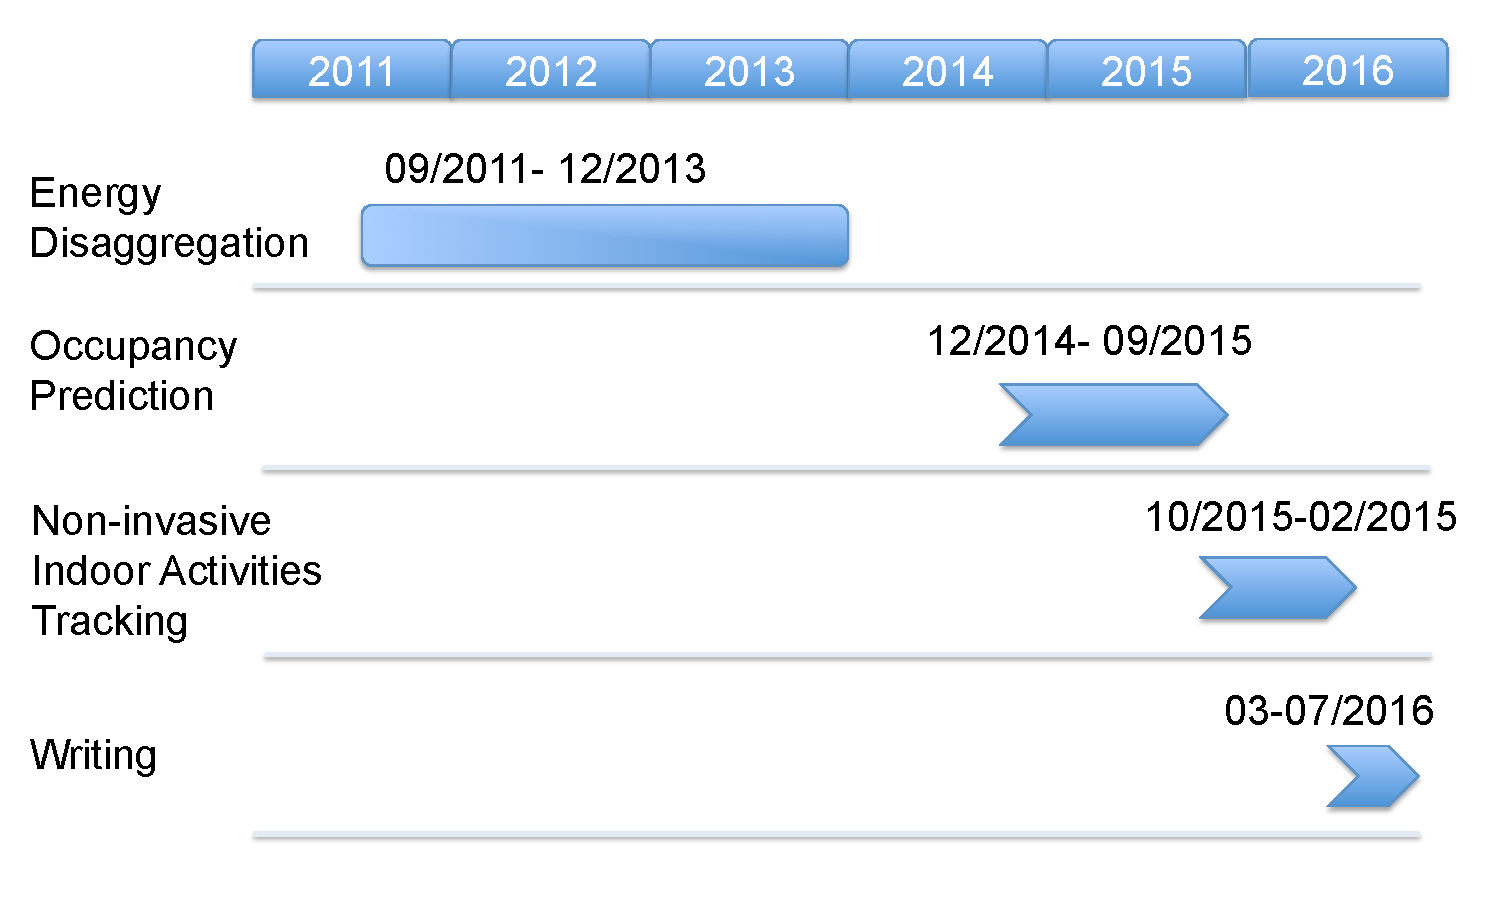
\includegraphics[width=0.8\textwidth]{fig/PhDTimeline.pdf}
%\caption{Timeline.\label{fig_PhDtimeline}}
%x\end{figure}

\chapter{Survey of Energy Disaggregation}
\markright{Huijuan Shao \hfill Chapter 2. Survey of Energy Disaggregation\hfill}
\section{Introduction}
Electricity usage permeates all aspects of modern society.
Its most conspicuous
uses include urban contexts such as
lighting, air conditioning, refrigeration, heating, and, powering
appliances and gadgets but its penetration is pervasive across rural
and industrial sectors.
In 2013, the residential and commercial sector
comprised nearly 40\% of all the electricity generated in the U.S.~\cite{energydatabook2011}.
Furthermore, our dependence on electricity will continue to grow
as emphasis shifts away from fossil fuel based vehicles to electric
vehicles.

While people generally agree on the importance of conservation and
usage curtailment, they are often at difficulties to quantify 
{\em where, when} and {\em how much} electricity is consumed.
Typically, residences and businesses receive
monthly electricity bills indicating aggregate usage, with no information on
the breakdown of consumption by appliances/devices, time of day, or day of
week (this is an area in great flux, however). Research has 
shown that simply making such feedback available to users
can reduce consumption by up to 50\%, although typical savings
are in the 9\% to 20\% range~\cite{energydatabook2011}.


%In modern society, people prefer a comfortable life at home,
%at work and  during leisure time outside.
%Energy, such as electricity, gas, bring us convenience in our daily lives.
%However, the use of energy causes environment pollution as well.
%Energy consumption increases continuously even faster than the population.
%One challenge we are facing is how to effectively
%save and easily manage energy usage at home \cite{cook2012smart},
%in office and in plants.

One obvious approach to determining the breakdown of consumption is to install
power meters in every circuit (and subcircuit)
to capture consumption of individual devices in homes and
offices. Such installation is costly and intrusive, making 
this option unviable in practice. 
An alternate
solution, called energy disaggregation or non-intrusive load monitoring
(NILM),
first proposed by Hart~\cite{hart1992}, is to use analytics to 
{\em infer} the breakdown of consumption from an aggregate 
power measurement of a
site. This drastically reduces the number of meters required per 
home/installation, typically to just one. Furthermore, depending on the analytics desired, it is possible to
use the measurements already being recorded by a utility meter for
disaggregation, especially in cases where utility companies have deployed
smart meters.

Energy disaggregation is hence today a booming area offering both
challenging problems for data analytics and having practical relevance in a
number of areas including sensor networks and building analytics.
Our goal in this paper is to provide a comprehensive survey of recent
advances in the area of energy disaggregation with a focus on the data mining
and machine learning algorithms used. 

%% The approaches applied to NILM not only discover the usage pattern of electricity, but also the techniques it uses can be applied to
%% water disaggregation  and
%% gas disaggregation \cite{froehlich2011disaggregated}.
%% Since this research helps conserve various resources from all perspectives,
%% it becomes more and more significant and popular in recent years.

\subsection {Background}

Hart~\cite{hart1992} first proposed the idea that power measurements at the
main electric meter in a home can be used to deduce what appliances are
turned on and how much electricity they are consuming.
Figure~\ref{fig_energyDisaggDefinition} (a) shows aggregate power measurement,
such as that at a main electric meter, from 10 am to 12 noon on a particular
day. The goal of energy disaggregation is to decompose this consumption into
its constituents as shown in Figure~\ref{fig_energyDisaggDefinition} (b),
which shows fourteen disaggregated devices. It shows that, for example, the
refrigerator turns on twice -- from 10:15 am to 10:40 am, and then from 11:50
am to 12:00 noon. At other times, the refrigerator stays off.

%shows an example of energy
%disaggregation by only recording the power usage of two main entry lines which
%are connected to a residential building \cite{kolter2010redd}. 
%\manishc{in fig 1 show two figures, the first with only the aggregate
%  consumption, the second with the disggregated components as you already
%  have. To make it fit, you can make the current figure shorter, perhaps
%  starting it around 10am (also put 'am' in the x-axis labels)}
%% Through disaggregation, we can find from Figure\ref{fig_energyDisaggDefinition} (b) that 
%% there are fourteen aggregated devices in total from 8:00am to 12:00am on a given day.
%% We aim to find out the status of these fourteen devices.
%% For example, the refrigerator is on during three periods: 8:50am to 9:05am,
%% 10:15am to 10:40am, and 11:50am to 12:05pm.
%% During other times, the refrigerator is off.


\begin{figure*}[ht]
	\centering{
    \begin{tabular}{cc}	
    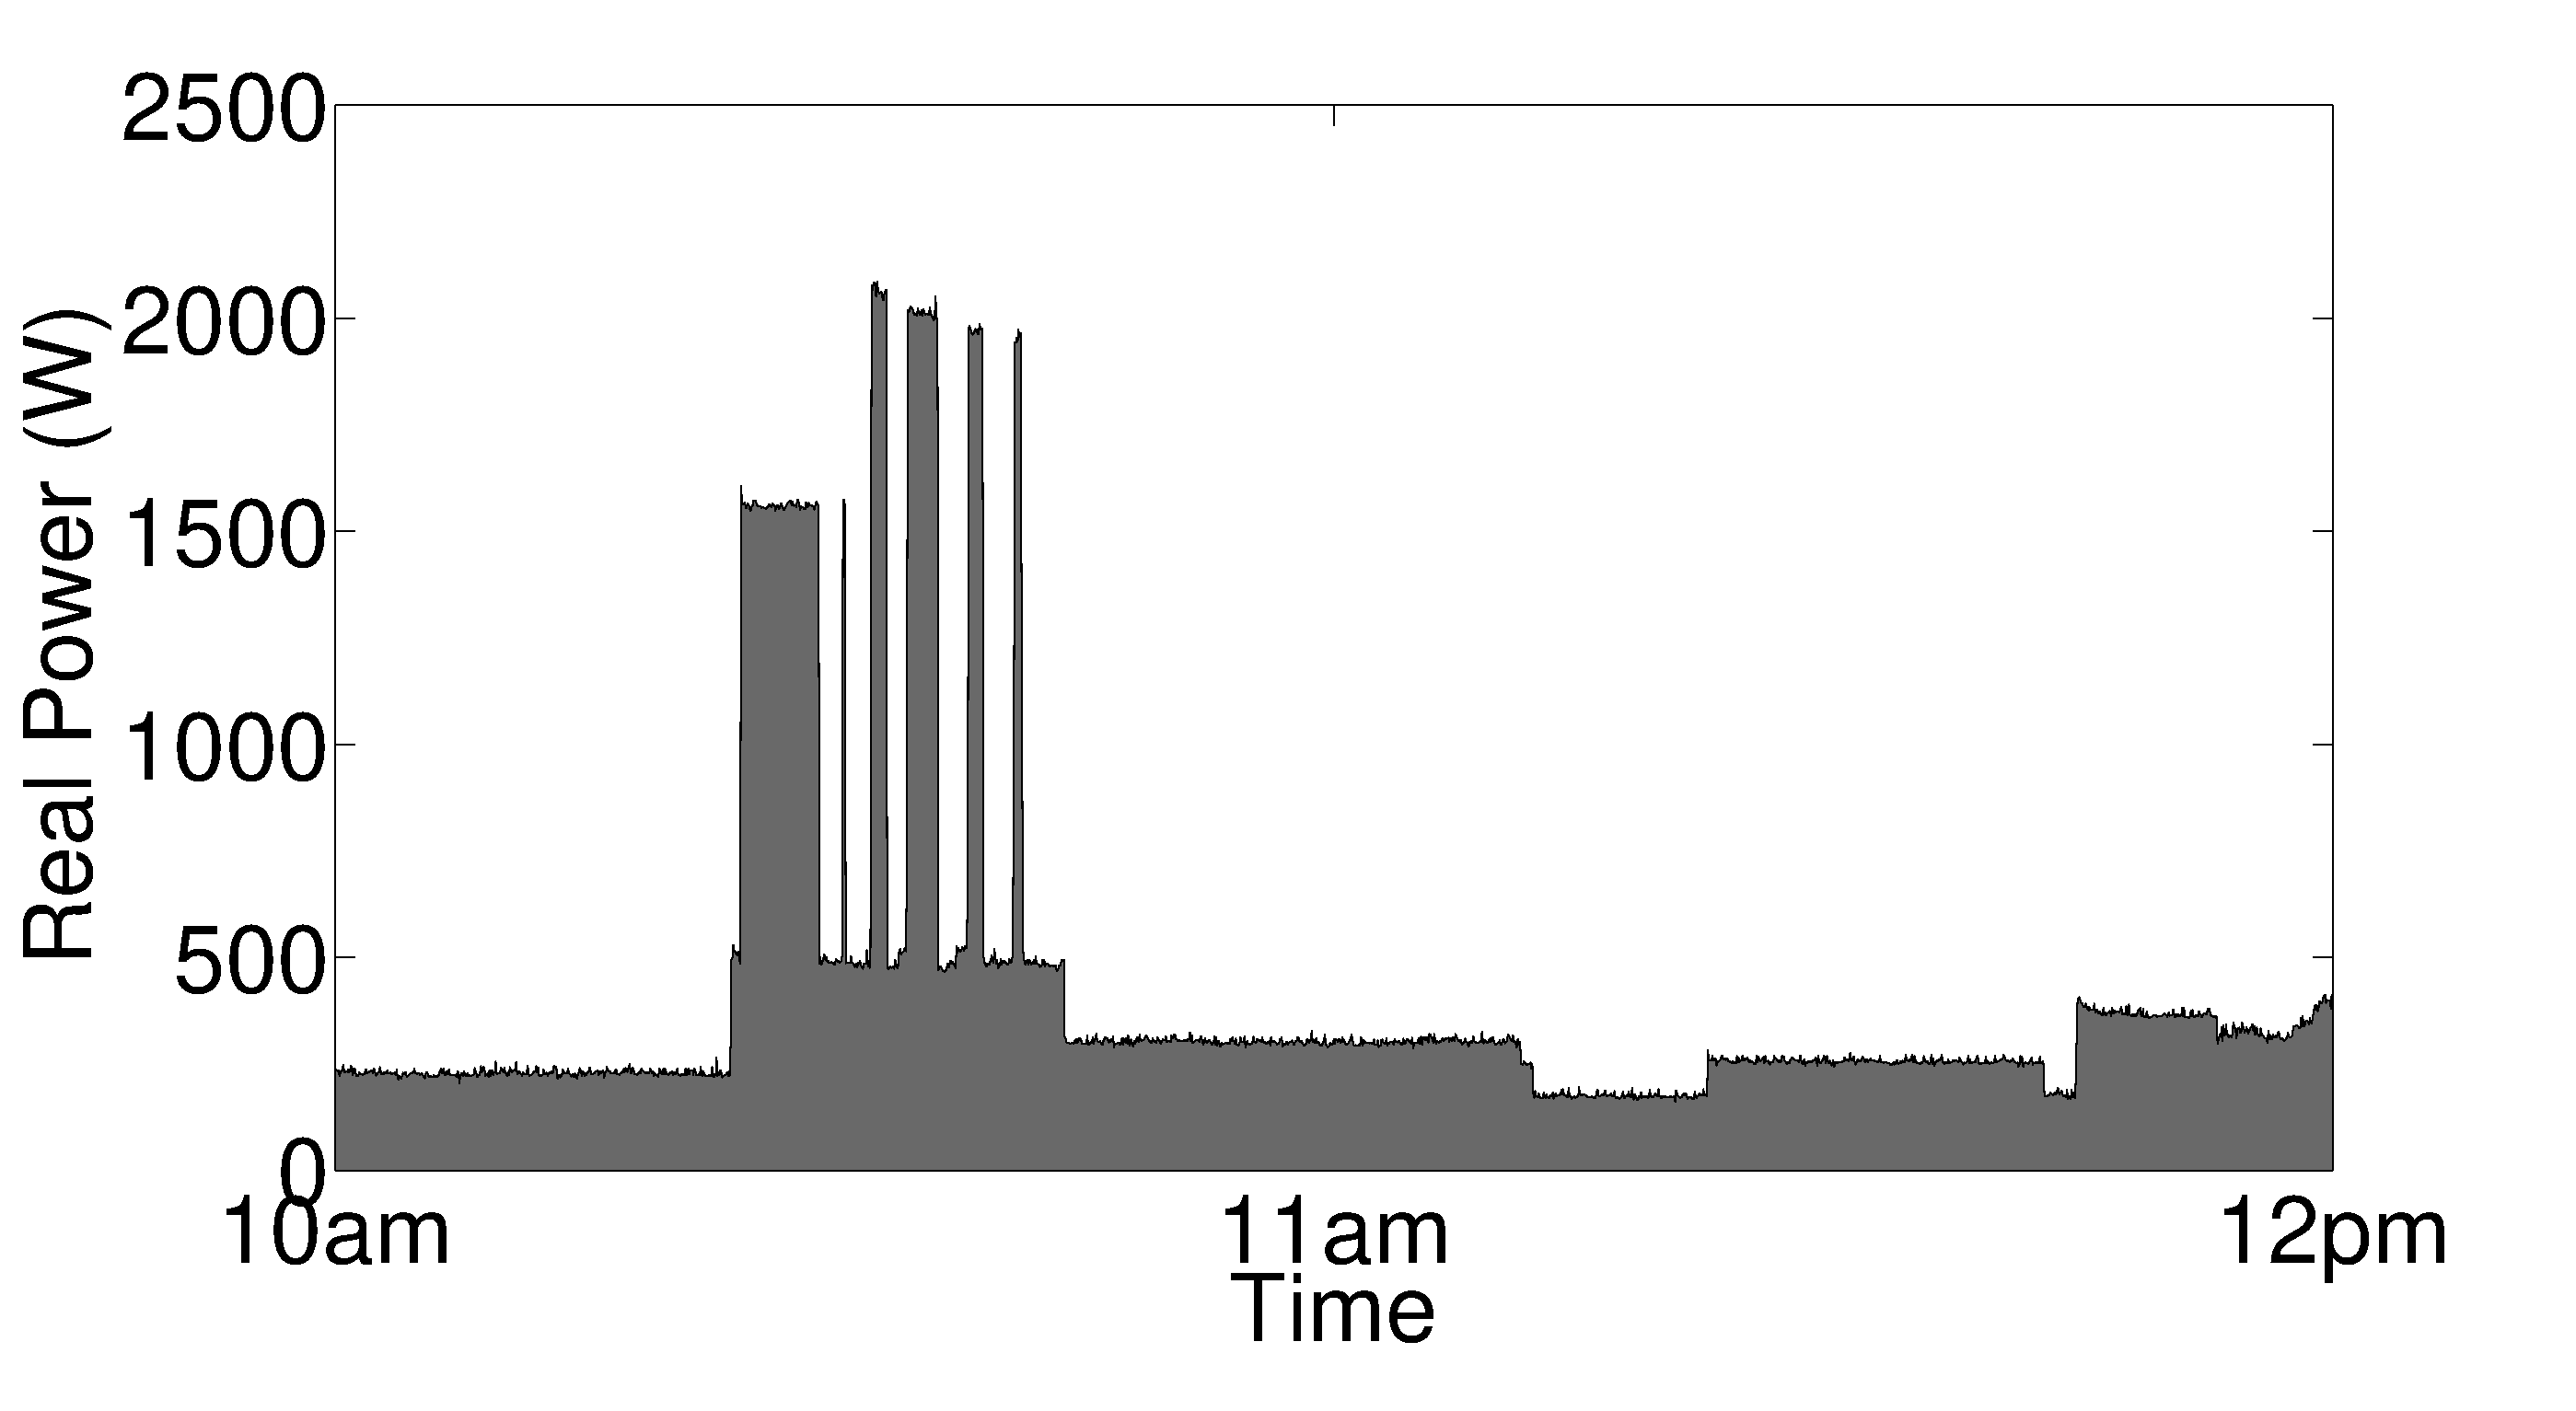
\includegraphics[width=0.5\textwidth]{figs/truth_agg.pdf}\hspace{1em}&
	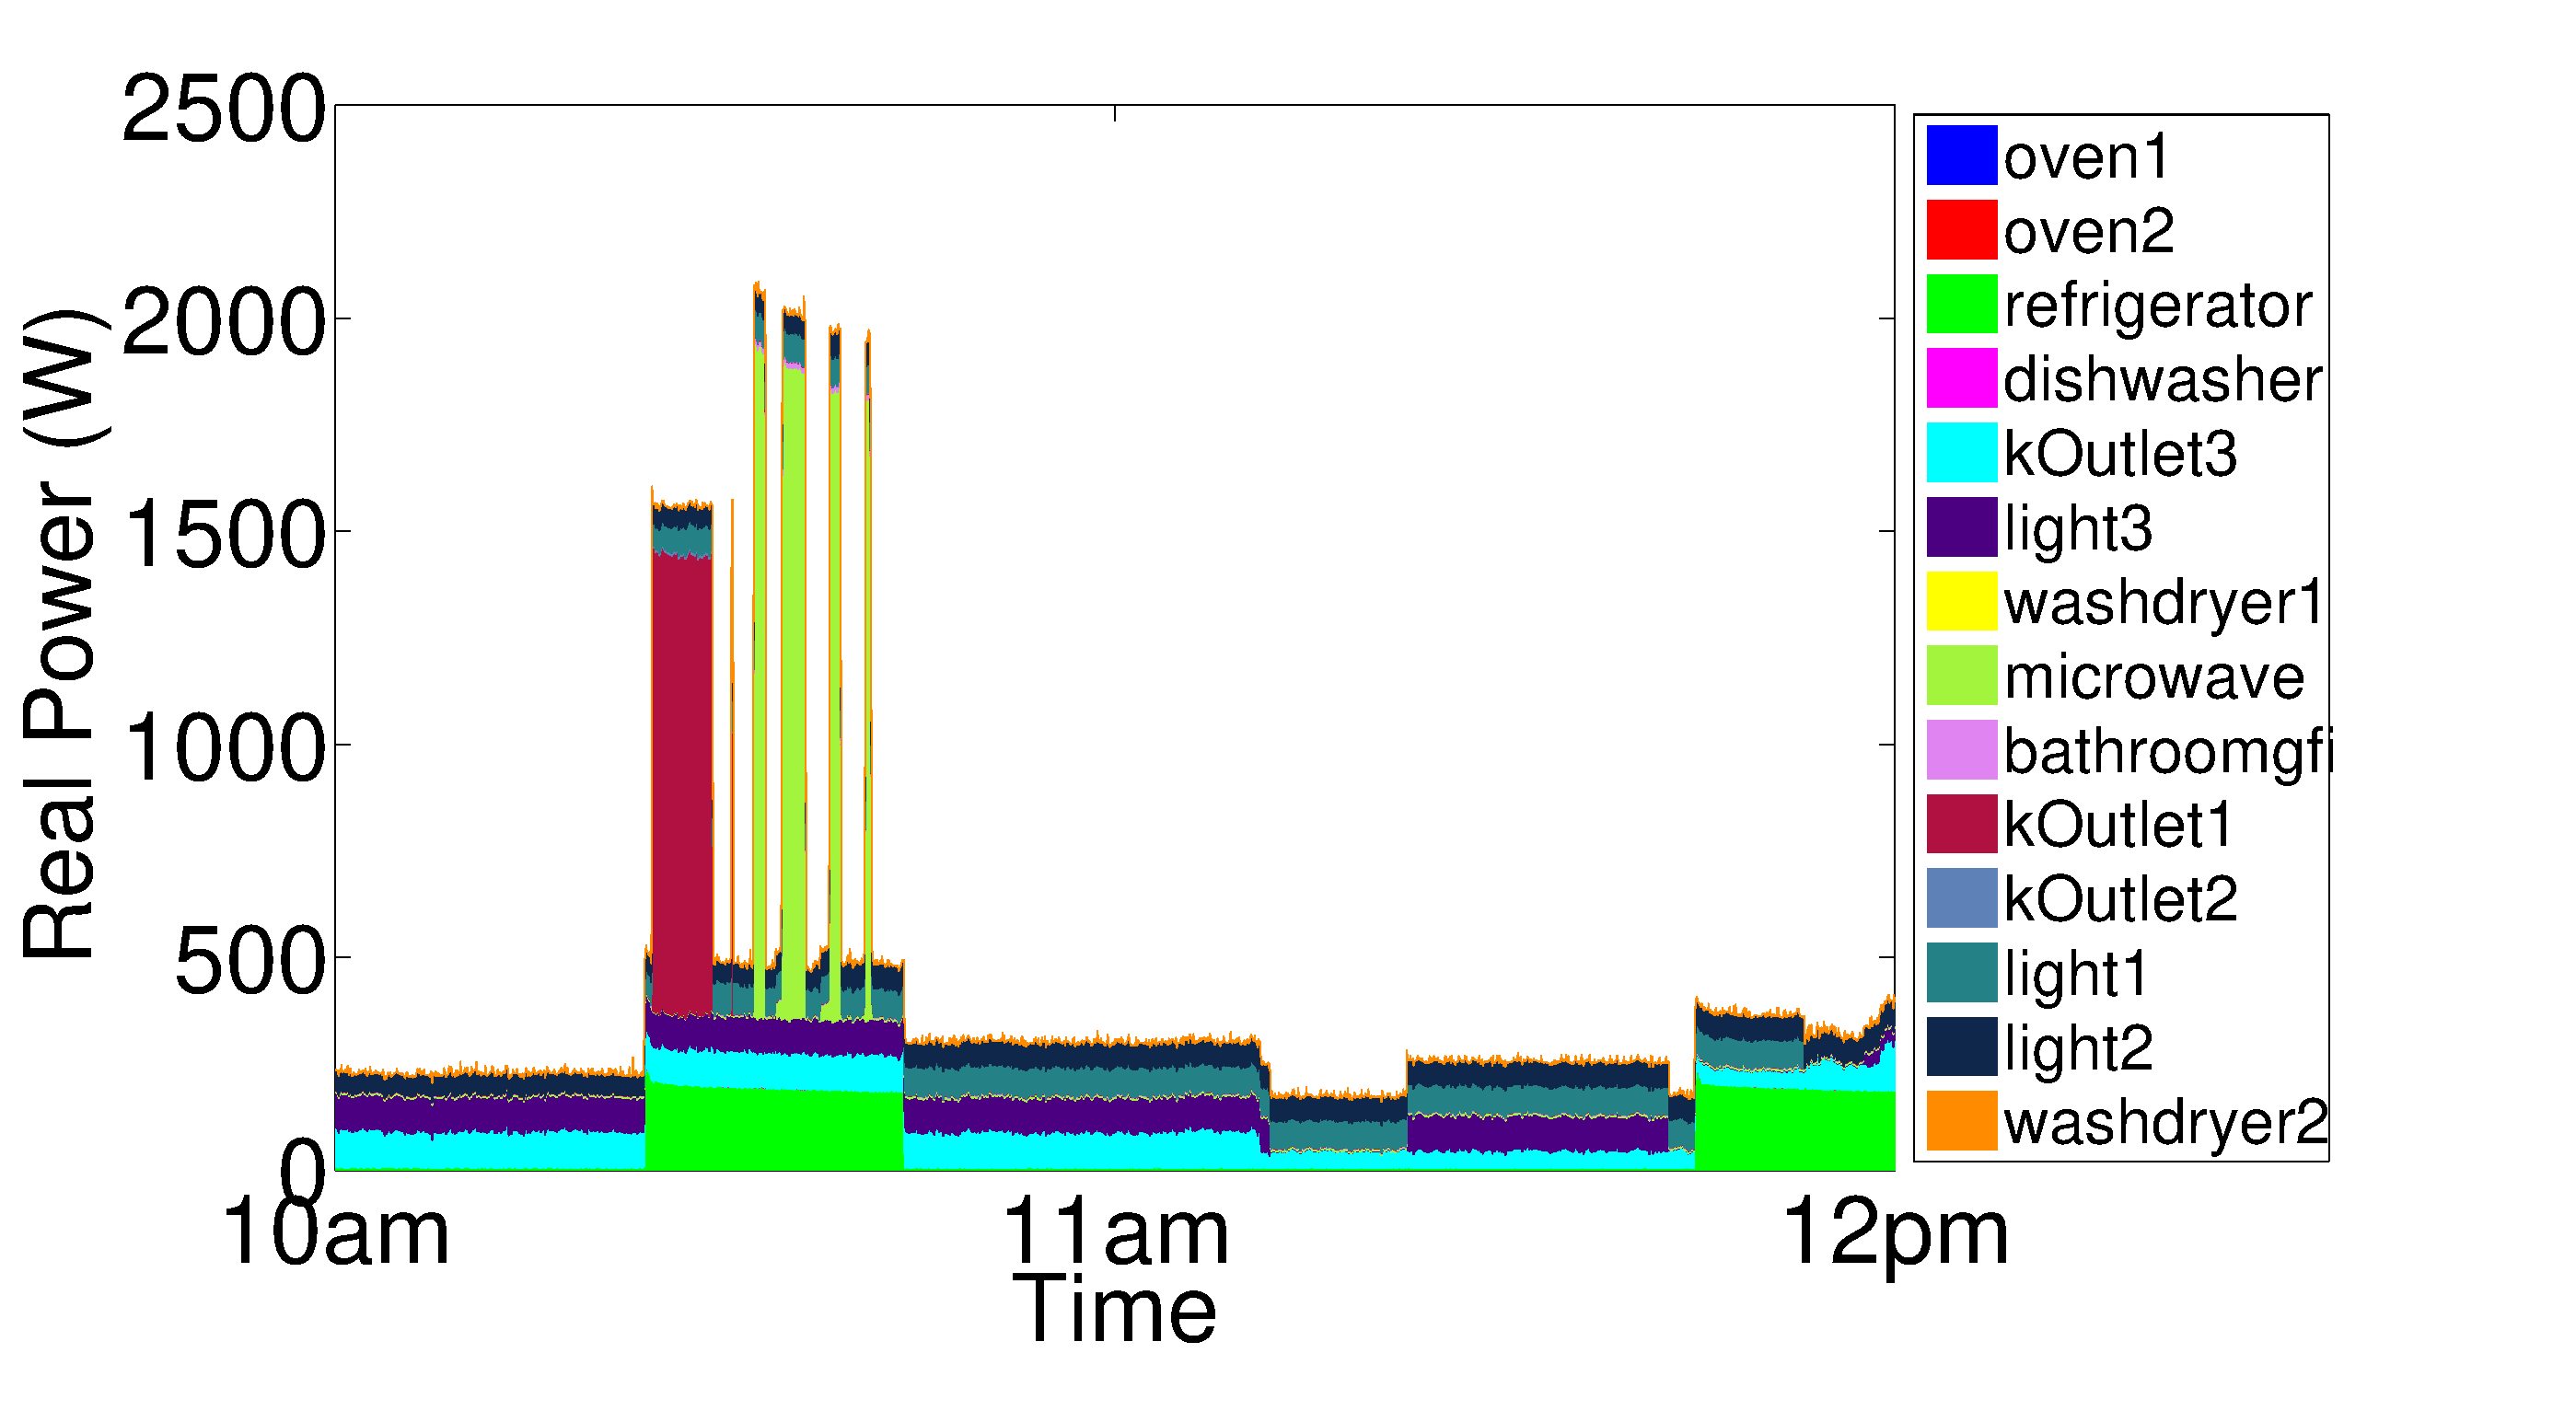
\includegraphics[width=0.5\textwidth]{figs/truth_disagg.pdf}\tabularnewline
   (a) & (b) \tabularnewline
    \end{tabular}
    }
	\caption{ (a) Aggregate power input to a disaggregation
algorithm. (b) Disaggregated information
about devices and their power usage patterns.}
	\label{fig_energyDisaggDefinition}
\end{figure*}

Energy disaggregation research can be understood in terms of 
the {\em features} that can be extracted from power measurements and
the underlying {\em algorithms} used.

One way to think of {\it features}
is in terms of
the sampling frequency
of meters. Low sampling frequency data is typically sampled at less than
$1$ Hz, while high sampling frequency data is sampled at higher than $1$ Hz.
Some features derivable from low frequency data are real power, reactive power,
low-order harmonics, and time of day. In addition to the ones inferable from
low frequency data, features from high frequency data include
many more characteristics such as harmonics, and current or voltage waveforms.

Another way to distinguish features is as transient vs steady state features.
Transient state features are only available from high frequency data. 
These features relate to transitory behavior seen in the current and voltage
waveforms when a device is turned on or off. 
On the other hand, steady state features are stable features that persist
after a device has changed its state. These
can be obtained from both low sampling frequency data and high sampling
frequency data. 

Yet another way to classify features is in terms of
AC power and non-AC power.
AC power characteristics are related to
current or voltage,
whereas non-AC power features include
power line noises, device correlation, and
contextual features like time or date, or weather information.

Initially, only
AC power features such as real power
and reactive power were studied~\cite{hart1992}.
With advances in electrical meter technology and availability of less expensive meters,
the transient state generated when a device turns on or off could be recorded and used
to identify devices~\cite{shaw2000PhdThesis}. 
Further, the raw current waveform~\cite{srinivasan2006neural}, voltage waveform~\cite{lam2007novel}, 
and the transform of the current waveform~\cite{chan2000harmonics}
can also be exploited as features.
Harmonics of non-linear devices
have also been studied~\cite{chan2000harmonics}.
Non-AC power features, such as power line noises~\cite{patel2007flick},
time of day, and device correlations~\cite{kim2011unsupervised}
are often combined with AC power features in modern systems. 

{\it Algorithms} applicable to energy disaggregation
can be categorized into supervised learning algorithms, 
unsupervised learning algorithms, and semi-supervised learning algorithms. 
%The applied data mining algorithms are composed of
%supervised learning algorithms, unsupervised learning algorithms
%and semi-supervised learning algorithms.
The supervised learning algorithms include
kNN methods~\cite{shaw2000PhdThesis},
support vector machines~\cite{patel2007flick},
neural networks~\cite{roos1994using},
genetic programming~\cite{baranski2004genetic},
sparse coding~\cite{kolter2010sparse}, 
as well as
combinations of supervised learning algorithms~\cite{nakano2007non}. 
Optimization algorithms used in the area of energy disaggregation have
been drawn from integer programming~\cite{suzuki2008nonintrusive}, 
dynamic programming~\cite{baranski2004detecting}, and
the Viterbi algorithm~\cite {zeifman2011viterbi}.
Unsupervised learning algorithms
have only been recently used in
 the last few years, and include
hierarchical clustering~\cite{gonccalves2011unsupervised},
factorial hidden Markov models (FHMMs)~\cite{kim2011unsupervised},
additive factorial approximate MAP (AFAMAP)~\cite{kolter2012aistat}, 
difference FHMM~\cite{parson2012nonintrusive}, 
and motif mining~\cite{shao2013temporal}.
Semi-supervised learning 
algorithms~\cite{lam2007novel,johnson2012bayesian} have also
been proposed.
%Because of the speciality of electricity,
%signal processing algorithm wavelet transform \cite{chan2000harmonics} is
%also an effectively adopted method.


\subsection {Challenges}
The field of energy disaggregation has evolved
over the last twenty years; while
some applications have achieved
qualified success, there are several challenging
problems that still need to be addressed before energy disaggregation can be
used more widely. Some of these problems include:

\begin{enumerate}
\item The number of devices is typically unknown and can only be
approximately estimated based on background information.

\item The number of power levels of each device is unknown.
Some devices such as lights may have only two steady states, viz. on and off.
Other devices  have several steady states.
For example, a microwave can operate in the states of defrost,
heat with low power, or heat with high power. Estimating
the exact number of states of a device is a hard problem.

\item Several devices may share the same real power and
it is hard to distinguish these devices from only the recorded aggregated
power values. 
For example, a light and a monitor could consume the same amount of real
power (e.g., around 38W). With more devices that share the same real power,
additional features are necessary to disambiguate among them.

\item Many devices may turn on or off at the same time.
A PC and printer likely turn on and off together, 
thus making it difficult to separate them from the aggregated power profile.

\item Instead of having a discrete range of power
levels, there are devices whose power consumption levels
   vary continuously, e.g.,
  variable speed devices (VSD), and lights with dimmers.
Once their power usage is aggregated with that from other devices, the
disaggregation problem becomes increasingly difficult.

\item Some devices are always on and seldom operated by
users. Because the operations on these devices are
rare, it is hard to identify these devices from prior historical data.

\end{enumerate}

The above problems are exacerbated in the case of commercial buildings.
While the voltage in residential buildings is typically $110$ or $220$ volts, 
the voltage in commercial buildings is
traditionally higher, at $208$ or $460$ volts.
Three-phase power is usually split
into single phase or two phases before reaching residential buildings.
In contrast, commercial buildings commonly use three phases.
Further, the devices in these two types of buildings are different.
Residential buildings
usually have devices such as microwaves,
refrigerators, ovens, lights, washers/dryers, and
air-conditioners.
The start-up duration of these devices
is short before they come to steady states.
Commercial buildings install more VSDs
including heating, ventilation, and air conditioning (HVAC) systems, 
variable-speed motor devices, and dimmable lighting. 
Further, banks of lights typically connect into a circuit together and
are powered on/off at the same time.

Generally, we face greater challenges in commercial buildings
than in residential buildings.
Norford and Leeb study non-intrusive load monitoring
challenges for commercial buildings~\cite{norford1996non}.
First,  load detection in commercial buildings is harder
because there are many devices powered on and off together.
Second, the start-up transient state of devices in commercial building is
much longer than those in discrete devices,
which dominate residential buildings.
Finally, in commercial buildings, reactive power is reduced to
make loads resistive, such as fluorescent lamp fixtures.

%The more devices connect,
%the possibility of case 2, case 3 and case 4 increases,
%the harder it is to disaggregate all devices correctly.

\subsection{Scope of this Survey}
Our objective is to provide an introduction to this space for a data
mining audience. While surveys exist on energy disaggregation,
e.g.,~\cite{zeifman2011nonintrusive},~\cite{liang2010load}, and~\cite{zoha2012survey}, they are mostly aimed at an electrical engineering audience and are
not suitable for data mining practitioners. Our survey provides both 
the background knowledge necessary and an overview of all aspects of
machine learning and data mining as applied to energy disaggregation.

In all survey papers, it is helpful to scope out what the survey does {\it not}
cover. The problem of disaggregation resurfaces in the
context of other utilities besides electricity, e.g.,
water~\cite{dai2011multi}, 
natural gas~\cite{froehlich2011disaggregated}, and music~\cite{schmidt2006nonnegative}. We do not cover these domains here and focus exclusively on electricity.
Second, there are many problems that appear related at first glance,
e.g., blind source separation~\cite{blumensath2005shift,davies2007source,lewicki2000learning} but are quite distinct from disaggregation. In the case of blind
source separation, the goal is to separate sources from at least as many
observations whereas in the case of disaggregation, only one aggregate signal
is provided. We do not cover these areas here.

\subsection{Organization}
The contents of this survey are organized as follows.
In Section~\ref{sec:basic}, we introduce some basic conceptions
of power, electricity, and electrical devices.
Next, in section~\ref{sec:problem},
we list several historical definitions of energy disaggregation
and present our working definition for the survey.
Characteristics which are used
to disaggregate devices are categorized in Section~\ref{sec:features}. 
It also describes how to setup an experimental testbed
and record necessary data with meters.
Section~\ref{sec:algorithms} summarizes a range of
algorithms that have been historically used for
energy disaggregation.
Section~\ref{sec:evaluation} takes up the important aspect of
defining evaluation measures for disaggregation.
Section~\ref{sec:ongoing} enumerates some tools, datasets, and software available to data mining researchers. Finally,
Section~\ref{sec:conclusion} identifies
promising research direction in this space.




%\section{Some Electricity for Data Miners}
\section{A Primer on AC power}
\label{sec:basic}
We will briefly review some background on concepts in AC power
before we describe algorithms for energy disaggregation.

\subsection{Electricity Transmission}
The power we use in our homes and offices is
generated at power plants and transmitted to buildings.
Figure~\ref{fig_powerconnection} illustrates how power
is transmitted and transformed.
%\manishc{Huijuan, did you adapt this figure from another source? (in which
%  case you may want to cite it)}
%\huijuanc{It is drawn by myself.}
Initially, a power plant generates 3-phase electrical power.
The voltage is stepped-up to several hundred kilo-volts for 
transmission.
In power substations, transformers decrease the
voltage. Usually after several substations,
the voltage is decreased to 4,800 volts as medium voltage power.
This medium voltage power is then split for two
different kinds of usage: residential and industrial.
To supply power for industrial or commercial buildings,
a 3-phase transformer changes the voltage to 208 volts or 460 volts.
Finally, a three-wire power service is delivered to end users.
To transmit power to residential buildings,
a 3-phase transformer again steps down the voltage.
The power is then transmitted by power poles, and
a power drum decreases voltage to around 110 volts
in the U.S. or 220 volts in other countries.
In the end, a 2-phase or 3-phase power service
is connected into a home for usage.
\begin{figure}
\centering
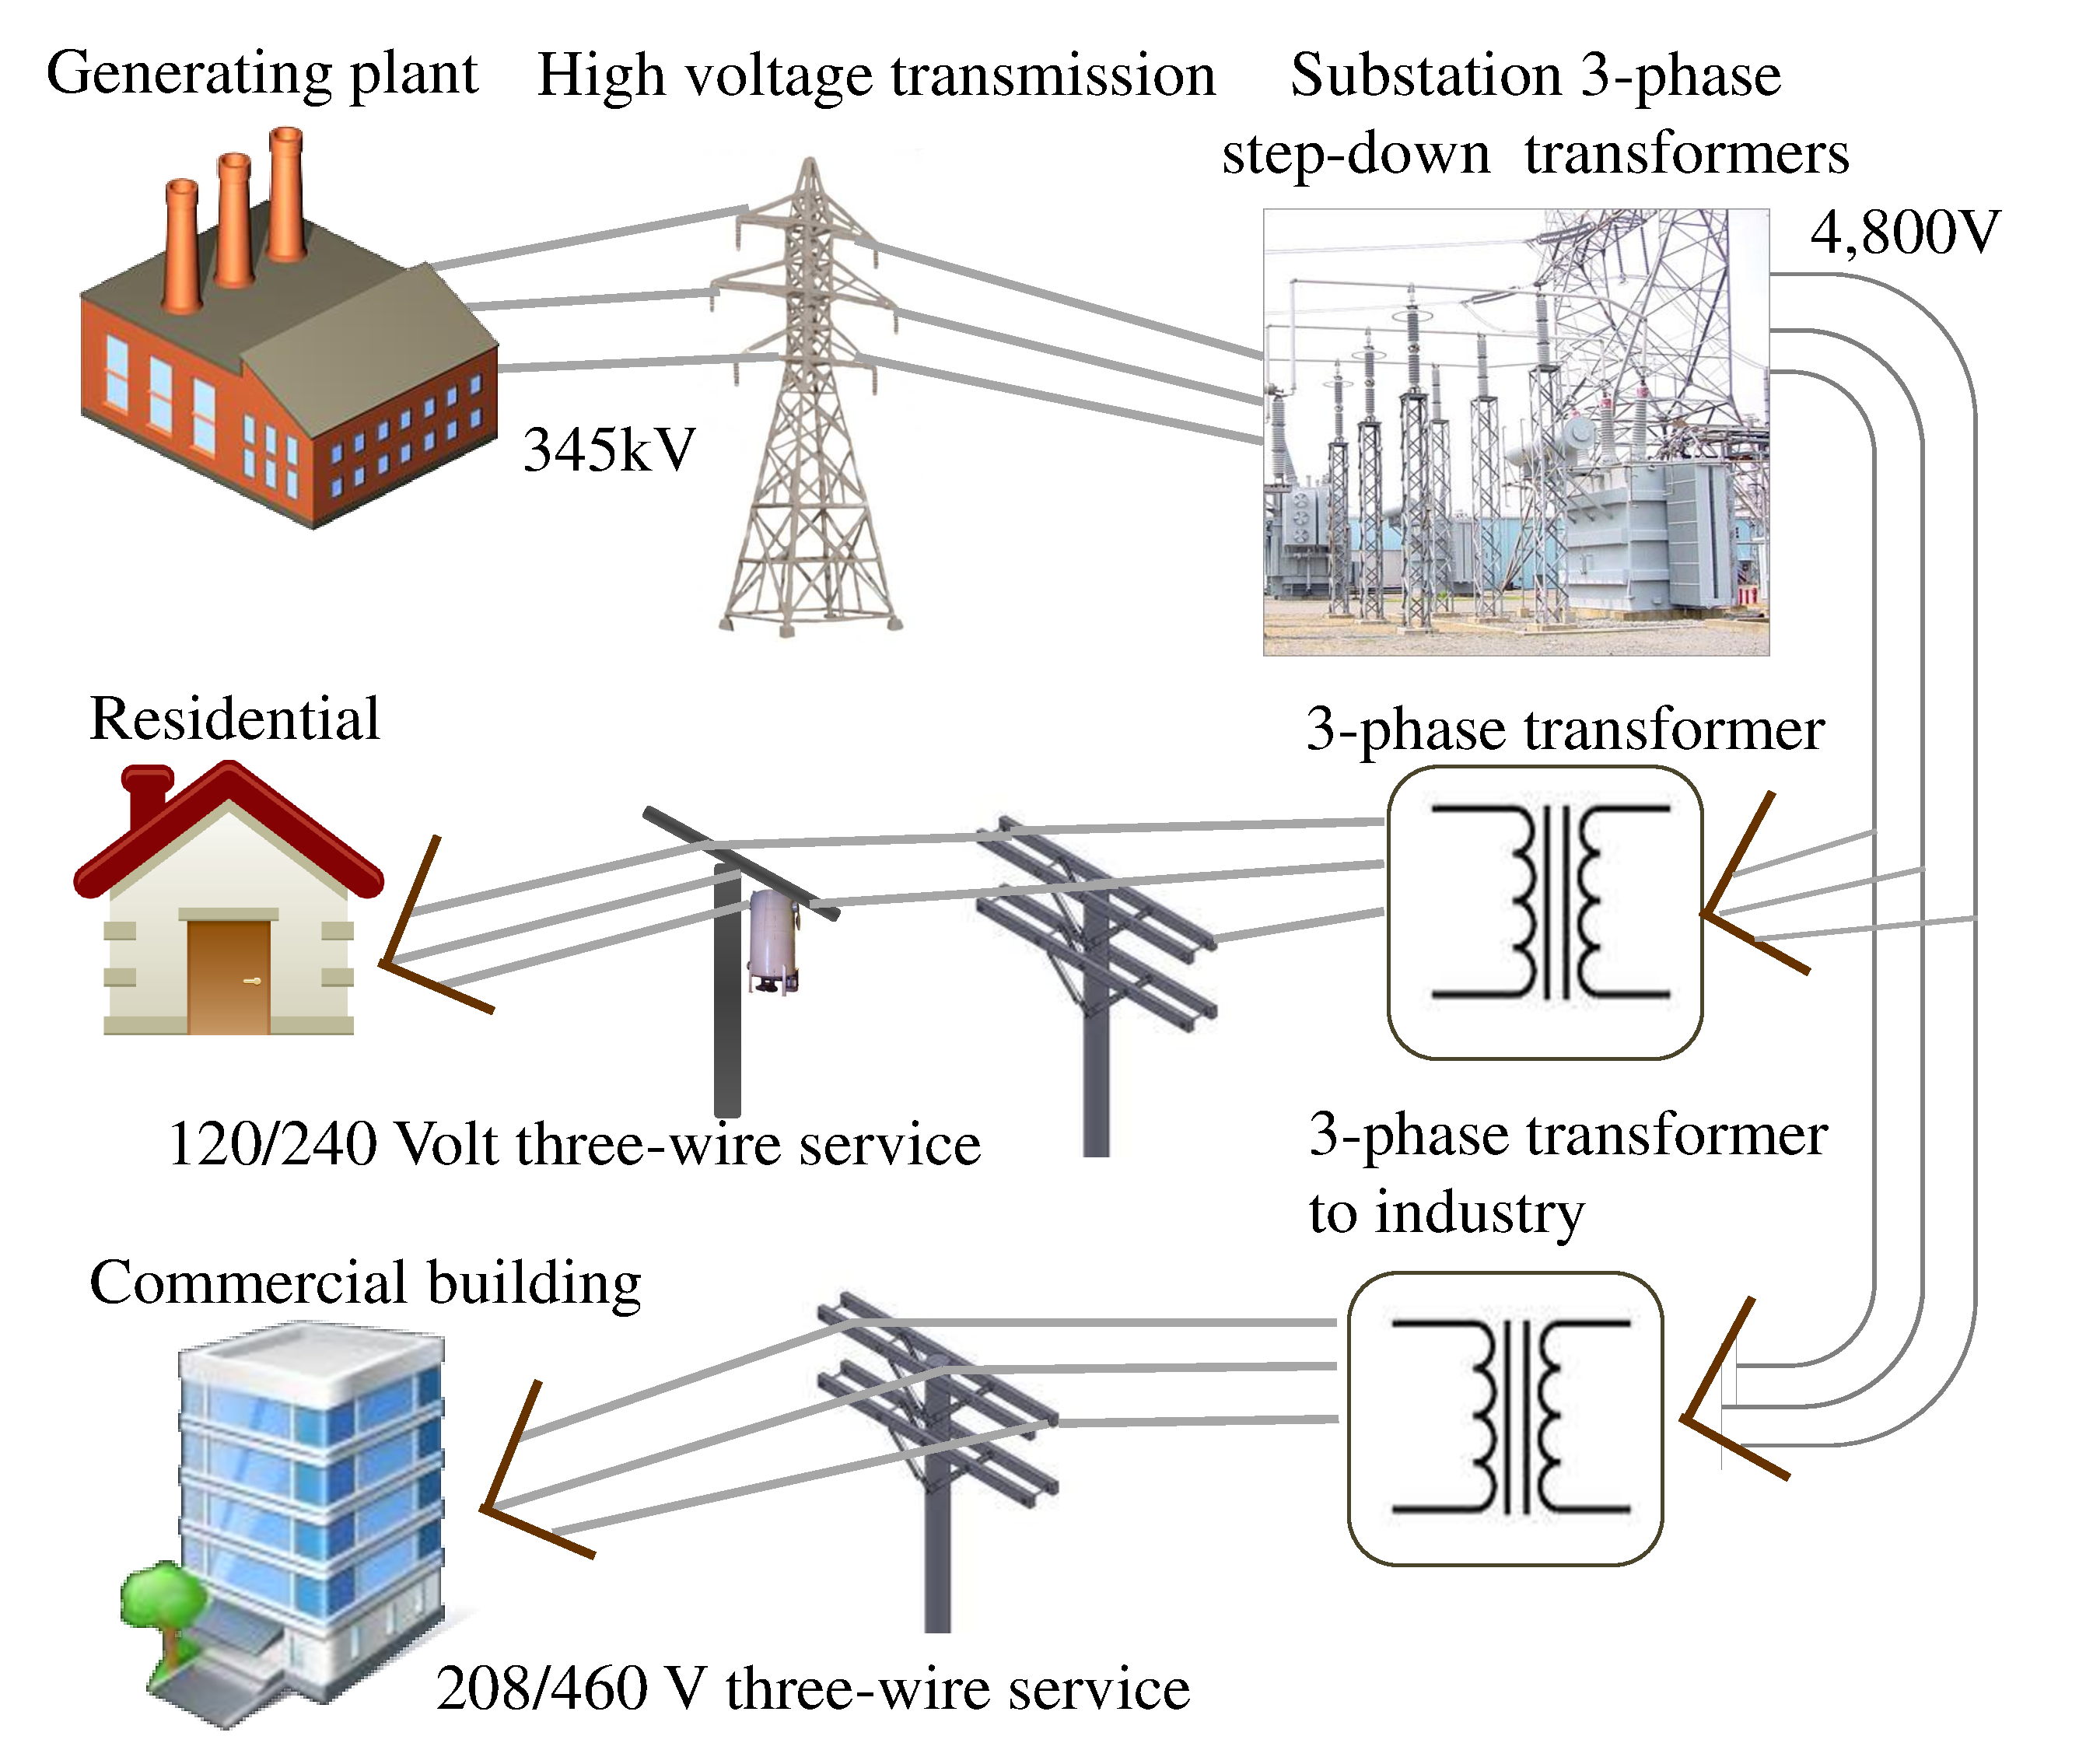
\includegraphics[width=4.5in]{figs/powerConnection.pdf}
\caption{Electricity generation and transmission to residential and commercial buildings.}
\label{fig_powerconnection}
\end{figure}


\subsection{Circuits and Devices}
Normally power in residential or commercial buildings
connects through two or three main phases.
Many circuits then draw power from these main phases
in parallel or in series.
\begin{figure*}[h]
	\centering{
    \begin{tabular}{cc}	
	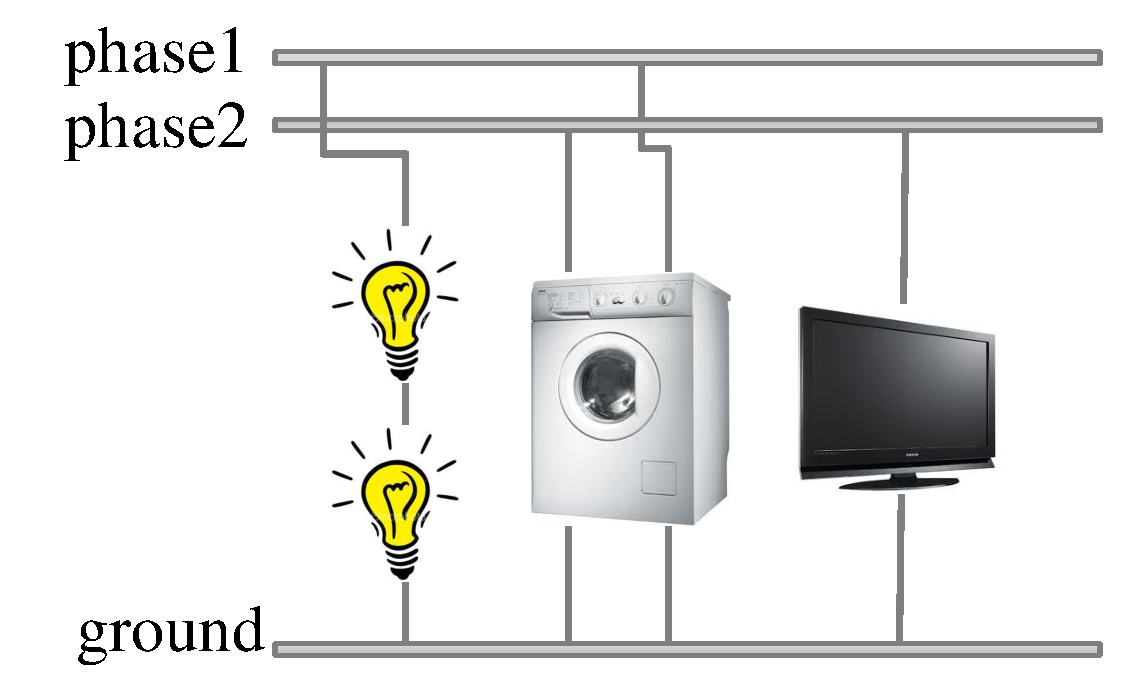
\includegraphics[width=0.43\textwidth]{figs/residentialBG.pdf} \hspace{1em}&
	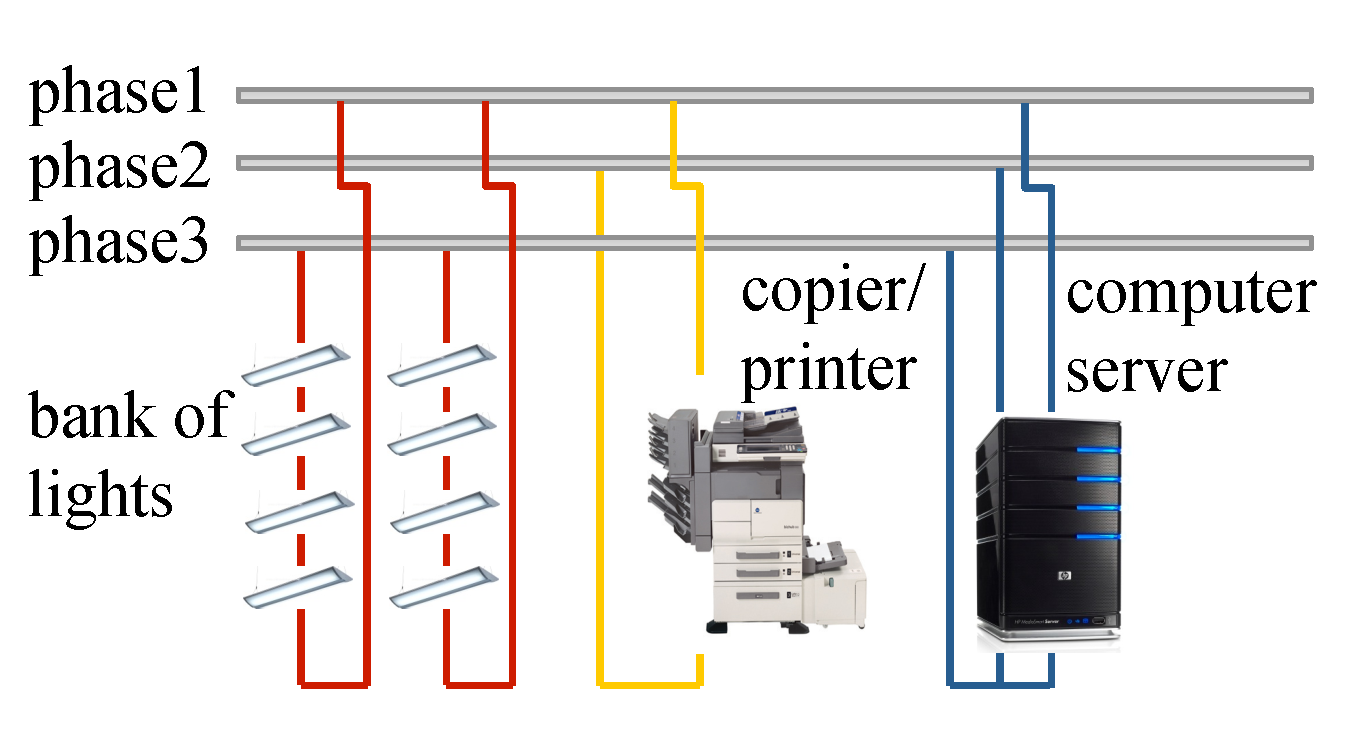
\includegraphics[width=0.5\textwidth]{figs/commercialBG.pdf}\tabularnewline
    (a) & (b) \tabularnewline
    \end{tabular}
    }
	\caption{Example of a circuit in (a) residential building and (b) commercial building.}
    \label{fig_residentialCommercialBG}
\end{figure*}

While most residential devices connect to a single phase some
heavy duty appliances require a two-phase connection.
Figure~\ref{fig_residentialCommercialBG} (a) depicts a typical connection
in residential buildings. 
There are two main phases: phase1 and phase2.
Three circuits connect into these two phases.
In the first circuit, two lights connect in series to phase1 and the ground.
In the second circuit, a washer/dryer connects to both phases.
In the third circuit, a television connects to phase2 and the ground.
Note that it is possible that several devices
connect to one phase in a circuit.

An example of
a circuit in a commercial building is
depicted in Figure~\ref{fig_residentialCommercialBG} (b).
Devices in any circuit connect to two or all of 
the three phases. 
%\manishc{what about three-phase load?}
%\huijuanc{update this figure: computer server connects to three phases.}
There are two circuits connecting to phase1 and phase3 in red.
Both these circuits supply power to a bank of lights (the lights
thus power on/off at the same time).
A copier/printer draws power from phase1 and phase2 in yellow. 
A computer server connects to all three phases in blue.

\subsection{Voltage and Current}
%After 3-phase or 2-phase voltage
%is made available to a building and 
%devices connect through these phases, 
%the power connection is effective for the building.
The voltage transmitted from
a power plant is typically 3-phase sinusoidal.
Figure~\ref{fig_threephase} depicts the
waveform of the three phases of AC power.
Each phase $V_1$, $V_2$, $V_3$ has a sinusoidal
voltage waveform. Between each phase,
there's a phase angle difference of $\pi/3$.
\begin{figure}[h]
\centering
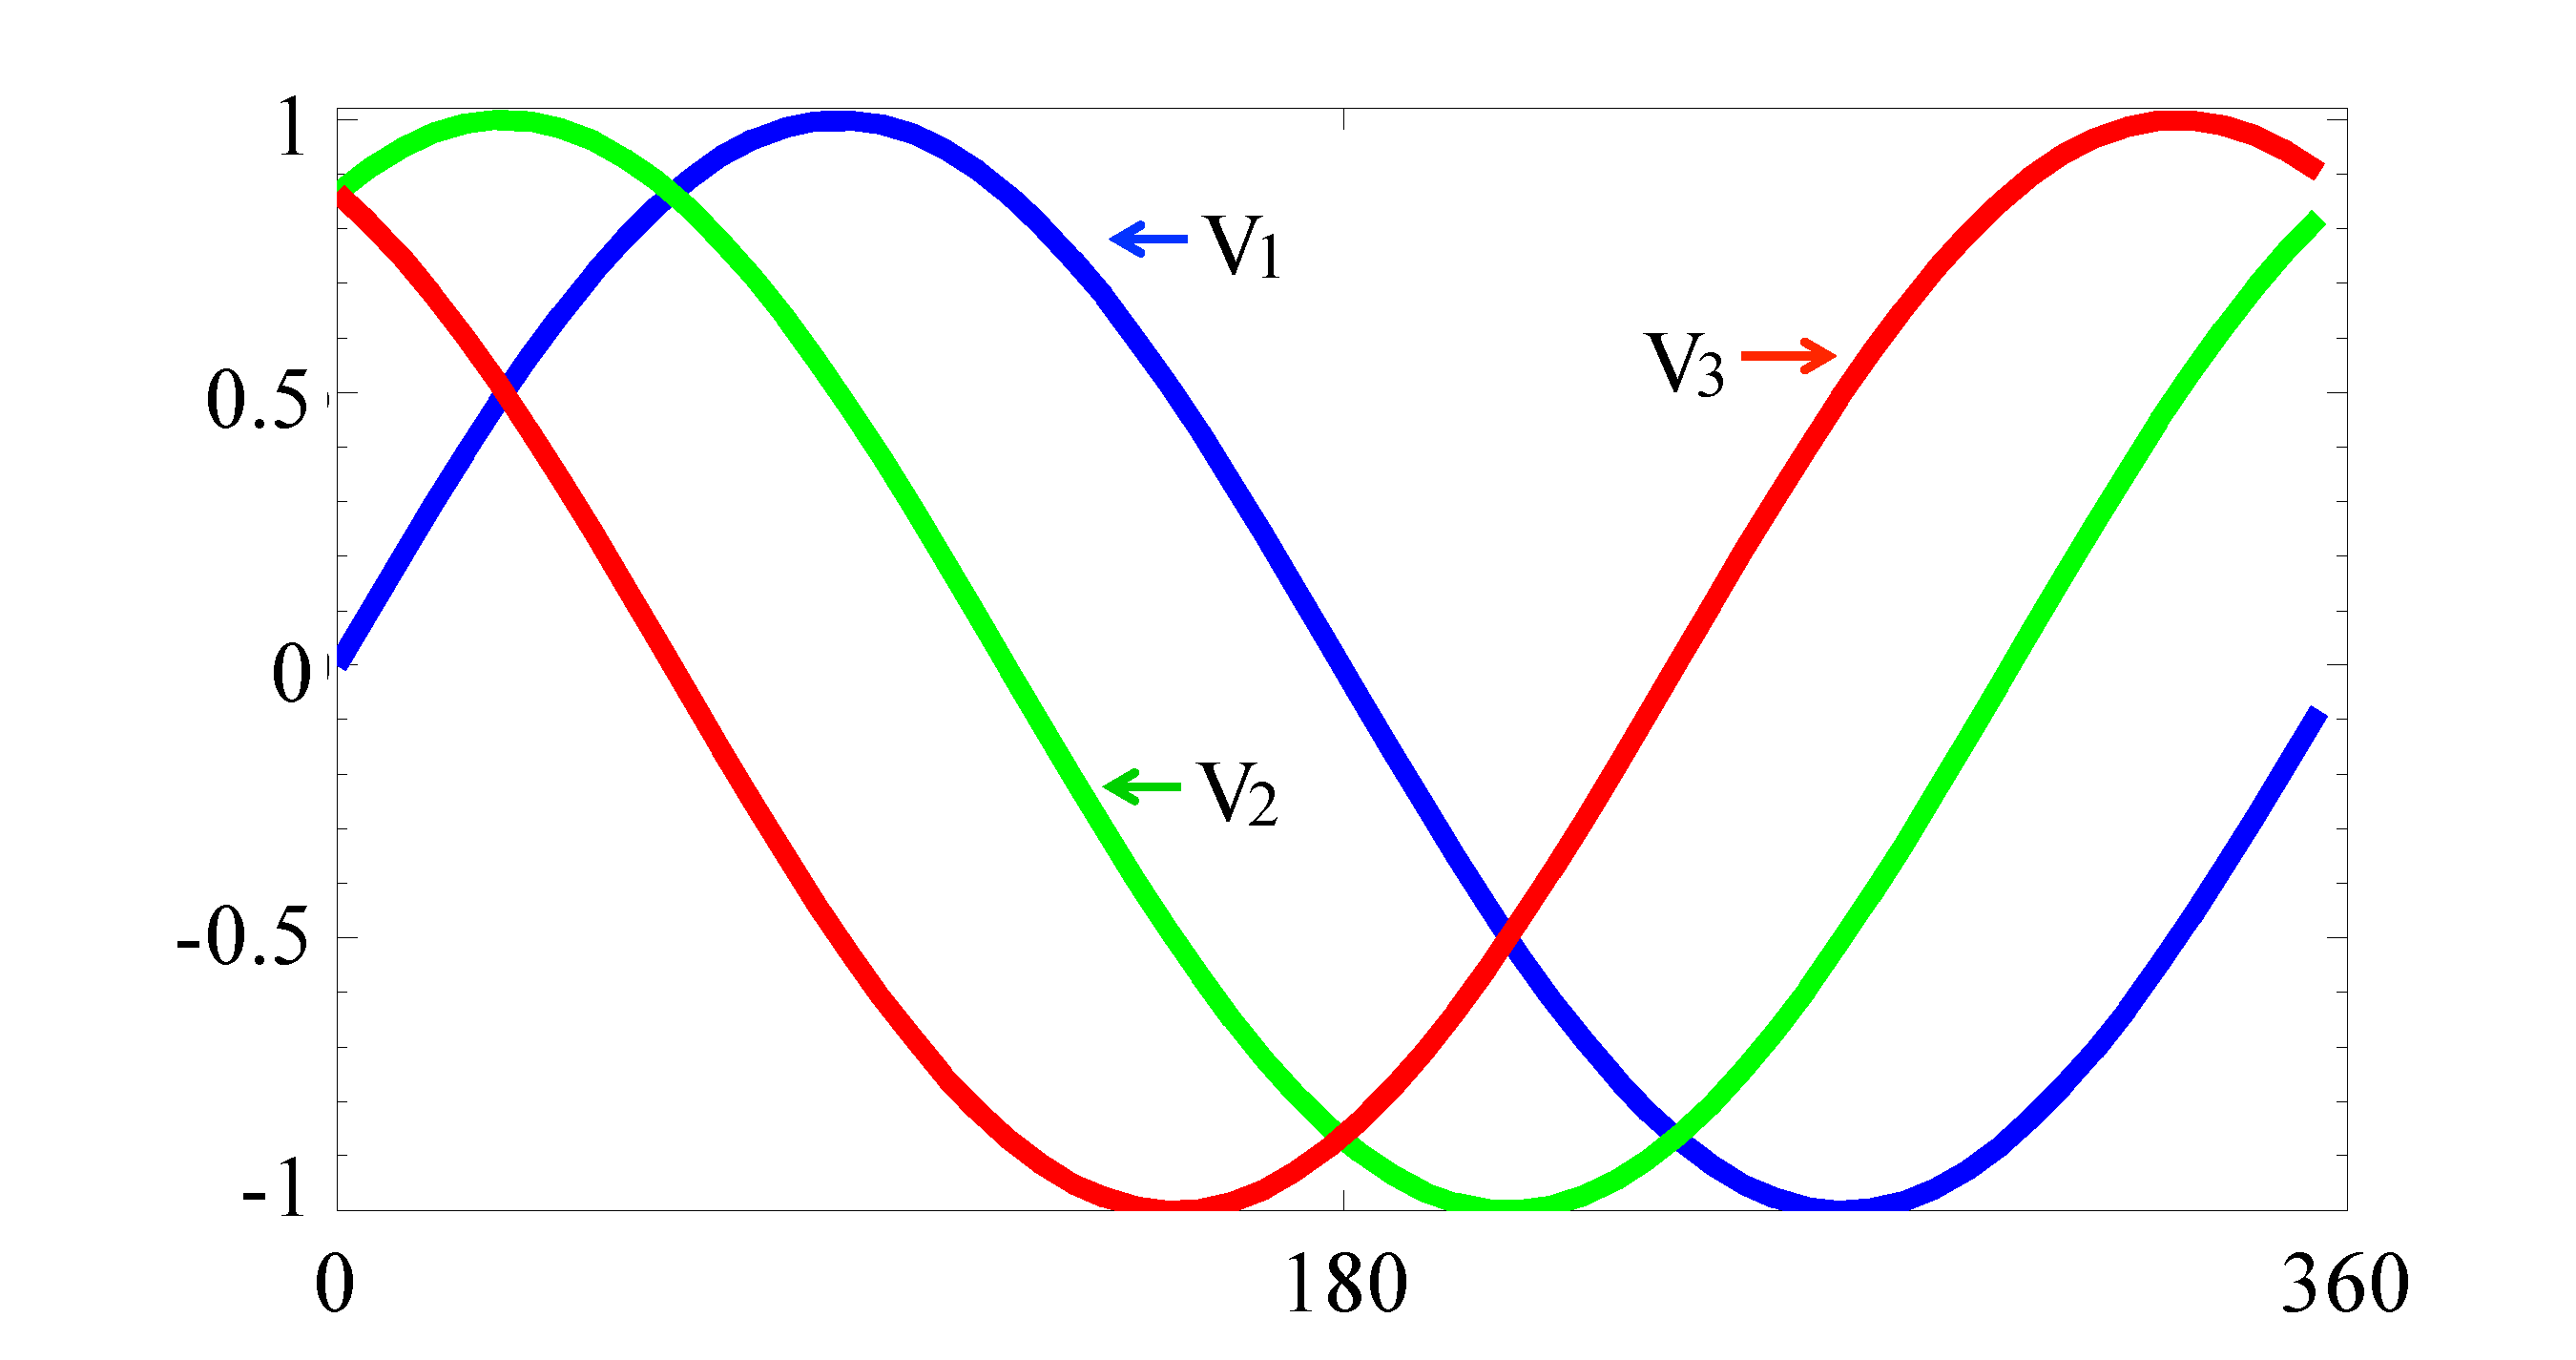
\includegraphics[width=0.4\textwidth]{figs/draw3phase.pdf}
\caption{Three phase power waveform.}
\label{fig_threephase}
\end{figure}


These three voltages can be represented mathematically
as the following three equations.
In these equations,
$\omega$ represents the frequency of
power. (While the frequency varies by country, it is 50 or 60 Hz in most 
places. For example, it is 60 Hz in the U.S.)

\begin{eqnarray*}
\label{eq_sinusoidal}
V_1&=& V\sin(\omega t) \\
V_2&=& V\sin(\omega t + \frac{2\pi}{3}) \\
V_3&=& V\sin(\omega t+\frac{4\pi}{3})
\end{eqnarray*}

%E can represent either voltage or current.
When a circuit is activated by a sinusoidal source voltage
with frequency $\omega$,
a current in this circuit is generated.
The relationship between current and voltage depends on
the impedance in the circuit.
Ideally, there are three types of impedance: resistor,
inductor, and capacitor.
Resistors draw power and generate heat.
An example of this is an electrical stove.
Capacitors store energy in an electrical field.
Inductors store electrical energy in a magnetic field.
Figure~\ref{fig_threebasicloads} shows three idealized AC circuits
with only resistor $R$ in the unit of ohm ($\Omega$), inductor $L$ in the unit of henry ($H$) or capacitor $C$ in the unit of faradays ($F$)
where $V_s(t)$ and current $i(t)$ are AC voltage and current.  
\begin{figure}[ht]
\centering
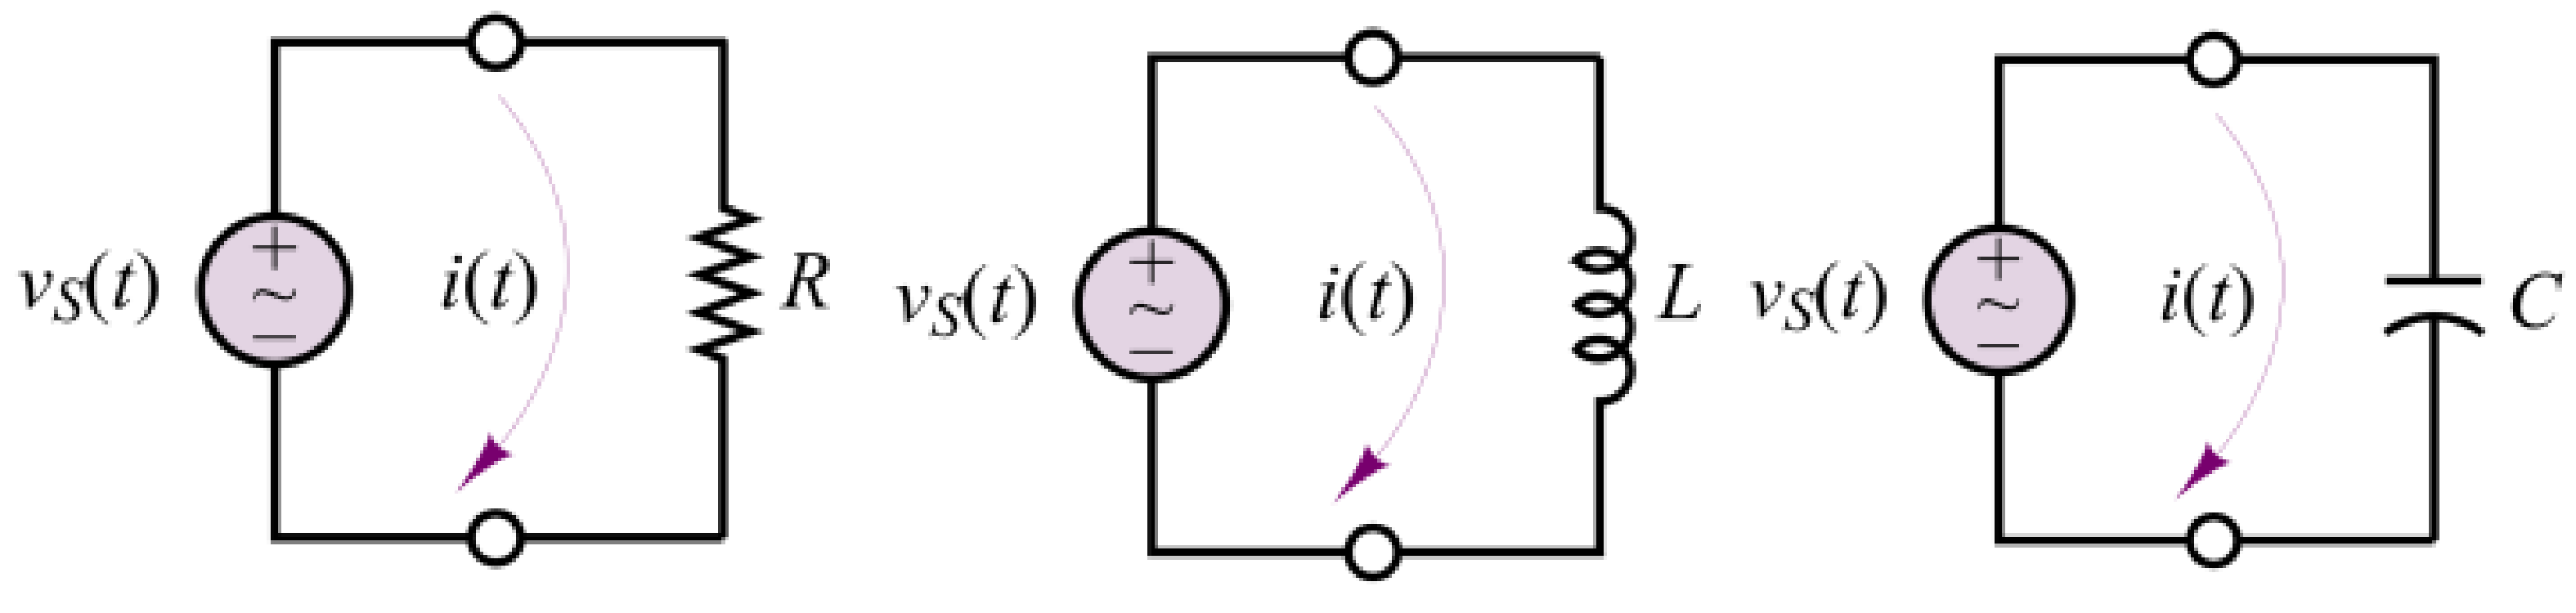
\includegraphics[width=3.3in]{figs/threebasicloads.pdf}
\caption{AC Circuit of basic loads: resistor, inductor, and capacitor (courtesy: \cite{eebook}).}
\label{fig_threebasicloads}
\end{figure}


The $i$-$v$ relationship for each circuit element of these
three types of impedance is described by the following formulas.
For the resistor circuit, according to Ohm's law $V=I R$,
\begin{equation}
i_R(t)=\frac{V_s(t)}{R}=\frac{A}{R}cos(\omega t).
\end{equation}
%The representative of R in Figure\ref{fig_simplecircuit}
%can be replaced by other loads.
For the inductor circuit, the relationship between current and voltage is
\begin{equation}
i_L(t)=\frac{A}{\omega L}cos(\omega t- \frac {\pi}{2})
\end{equation}
For the capacitor circuit, the relationship between current and voltage is
\begin{equation}
i_C(t)= \omega CAcos(\omega t + \frac {\pi}{2})
\end{equation}
where $A$ represents the amplitude, 
and $\omega$ denotes the frequency.

%\manishc{some of the symbols are not defined here. also, you use E for voltage
%  in the previous equations, and use V here.}
%\huijuanc{the symbols are explained in the above paragraph. The voltage symbol is unified as V.}  
In practice the impedance of any electrical device is composed of
at least one of these three types: 
resistors, inductor, and capacitor.
A device may include several resistor units or
inductor units or capacitor units.
For example, the mainboard of a computer 
typically contains a number of capacitors.

%%%%%%%%%%%%%%%%
\subsection{Real Power and Reactive Power}
\label{sec_pvCalculation}
In the field of electrical engineering,
real power and reactive power are concepts used
to characterize the power consumption of electric devices.
Meters typically measure current in amperes (A),
voltage in volts (V),
real power in watts (W) and
reactive power in volt-ampere reactive (VAR).

A scatter plot of real power and reactive power for different devices
is given in 
Figure~\ref{fig_realReactive_hart1992}.
The water heater, IR light, and fan only consume
real power (no reactive power) because
these devices are composed exclusively of resistors.
The values of real power of these three devices
are different from each other.
The refrigerator and water pump have similar reactive
power at around 450 VARs, but their
real power values are 750 W and 250 W, respectively.
\begin{figure}[ht]
\centering
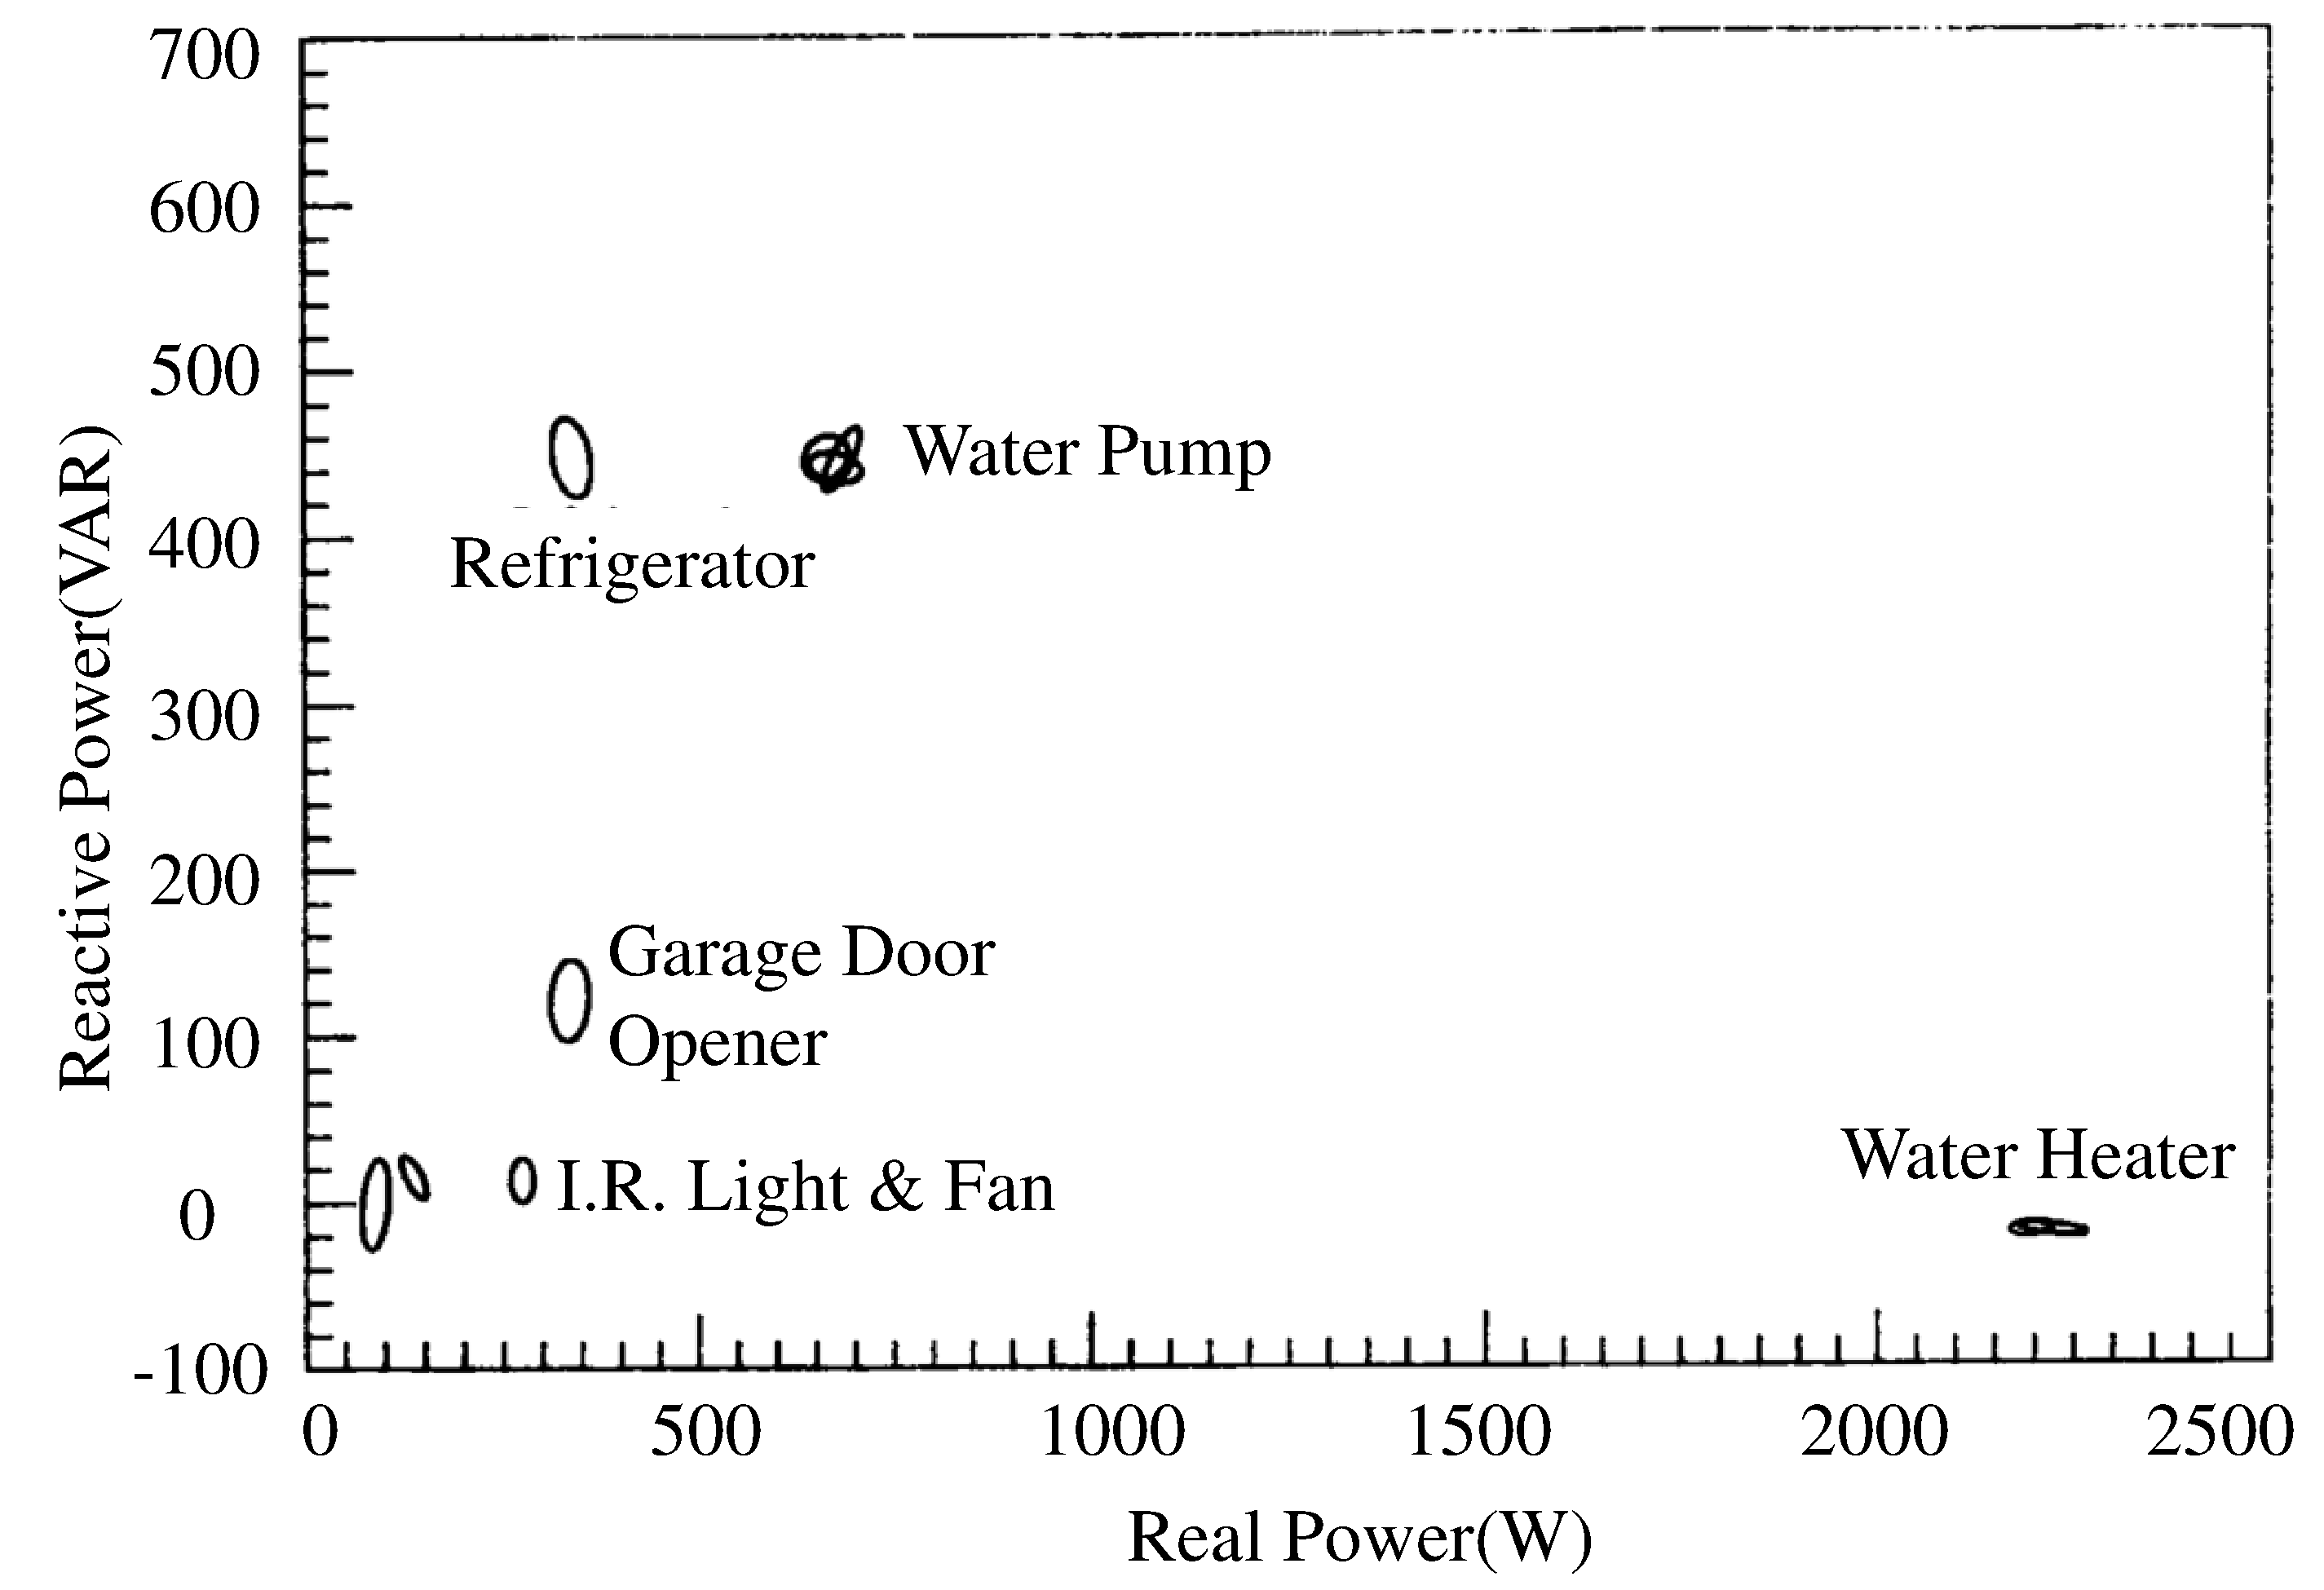
\includegraphics[width=4in]{figs/realReactive_hart1992.pdf}
\caption{Real and reactive power for different devices (courtesy: \cite{hart1992}).}
\label{fig_realReactive_hart1992}
\end{figure}


Real power and reactive power values can be
obtained by the values of voltage, current, frequency of AC power and the phase angles of voltage and current. 
Suppose we have voltage, $v(t)= V cos(\omega t - \theta_V)$ and current, $i(t)= I cos(\omega t - \theta_I)$,
%\begin{eqnarray*}
%\label{eq_voltageCurrent}
%v(t)= V cos(\omega t - \theta_V) \\
%i(t)= I cos(\omega t - \theta_I)
%\end{eqnarray*}
where $\omega$ is the base frequency of AC power,
$\theta_V$ denotes the phase angle of voltage and
$\theta_I$ represents the phase angle of current.
Then, the instantaneous real power at time $t$ is given by:
\begin{equation}
\label{eq_insPower}
P(t)= v(t) \cdot i(t)
\end{equation}
The average root mean squared (RMS) real power usage over a period of time is typically what is
used to measure power consumption in our electricity bill.
Assume $V$ and $I$ represent the maximal value of voltage and current, then
$V_{rms} = \tilde{V} = \frac{V}{\sqrt{2}}$ and $I_{rms} = \tilde{I} = \frac{I}{\sqrt{2}}$.
The average power $P_{av}$ is the inner product of voltage and current $P_{av}=\tilde{V}\tilde{I}cos\theta$, 
where $\theta$ is the phase difference between voltage and current,
i.e. $\theta= \theta_V - \theta_I$.

%It is calculated as Equation.\ref{eq_rmsPower}.
%\begin{subequations}
%\begin{align}
%V_{rms}&=& \frac{V}{\sqrt{2}} \\%= \tilde{V} \\
%I_{rms}&=& \frac{I}{\sqrt{2}} \\%= \tilde{I} \\
%P_{av} &=& \tilde{V}\tilde{I}cos\theta \label{eq_rmsPower}
%\end{align}
%\end{subequations}
%where .
%$P_{av}$ is the average power generated by voltage and current.

%$\tilde{V}$ and $\tilde{I}$ are the RMS value of voltage and current.

The relationship between real power and reactive power is summarized in
Figure~\ref{fig_powerTriangle} and by
Equation (\ref{eq_powerTriangle}).
\begin{subequations}
\begin{align}
S=\tilde{V}\tilde{I}cos\theta+ j\tilde{V}\tilde{I}sin\theta \\
S=P_{av}+j Q \label{eq_powerTriangle}
\end{align}
\end{subequations}
\noindent
where $S$ is the apparent power,
$P$ is the average real power,
and $Q$ is the reactive power.

\begin{figure}[ht]
\centering
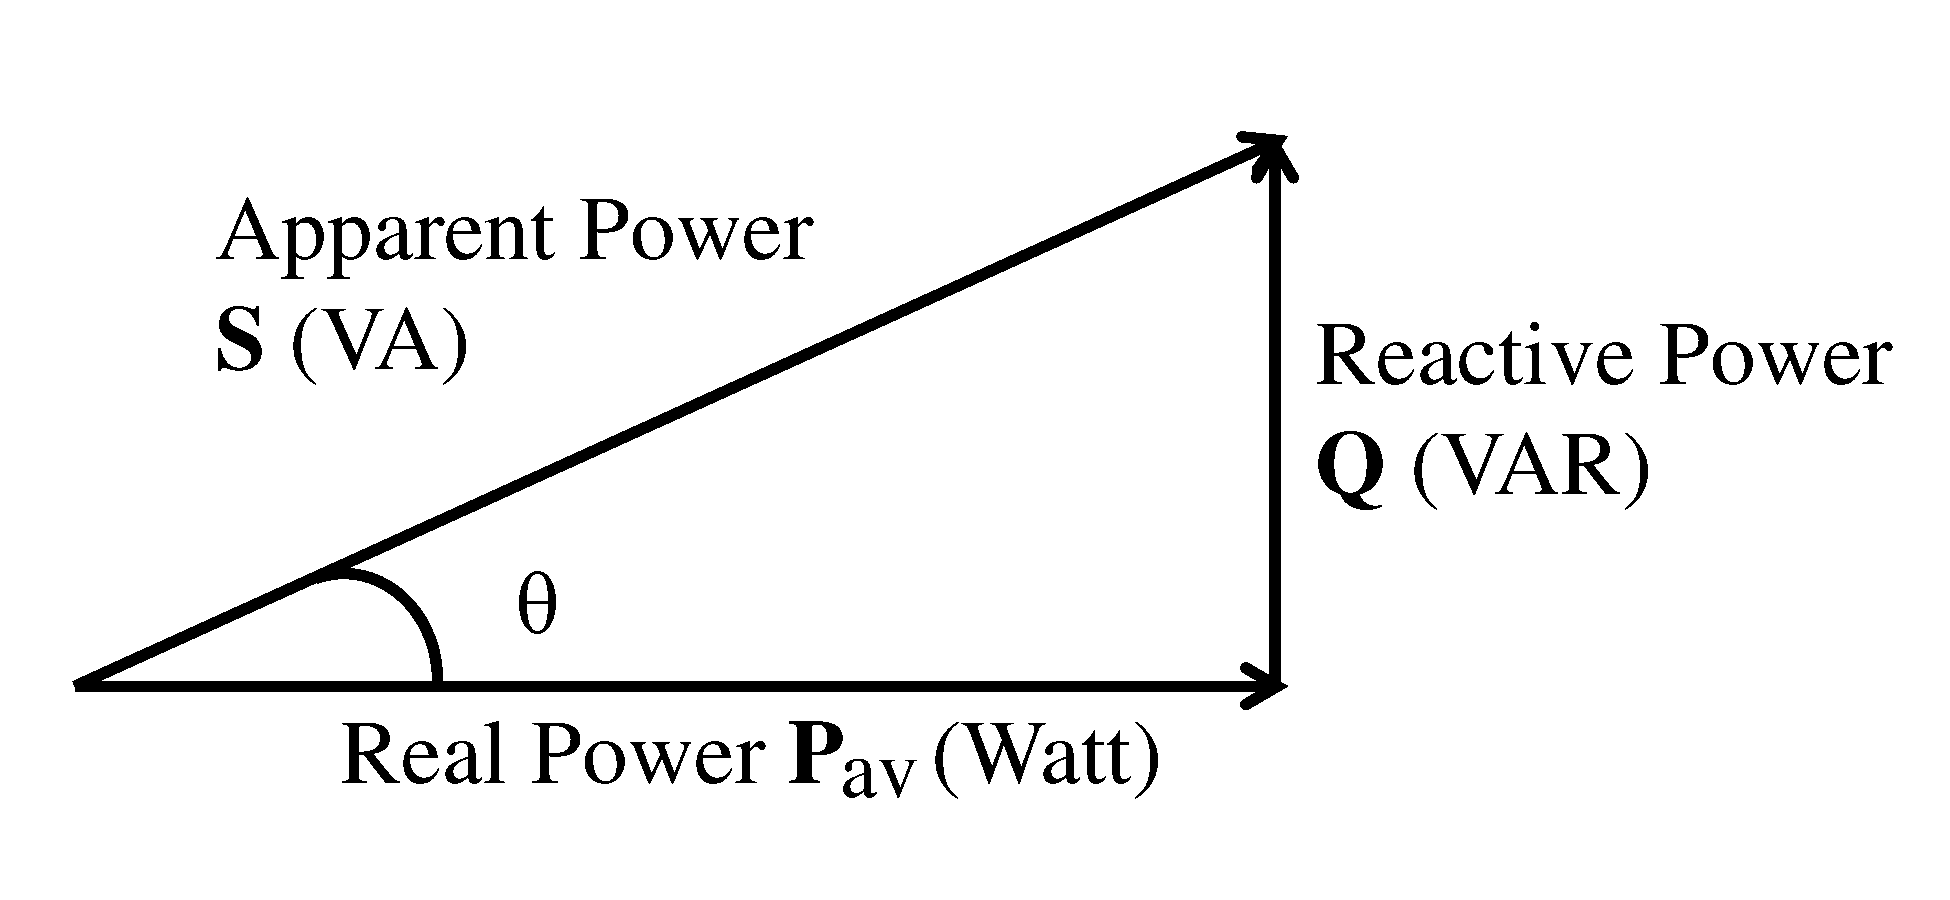
\includegraphics[width=1.8in]{figs/powerTriangle.pdf}
\caption{Power Triangle.}
\label{fig_powerTriangle}
\end{figure}


From Figure~\ref{fig_powerTriangle},
we can calculate the power factor, $\cos\theta$.
For resistive devices, the power factor is equal to 1,
which means there is only real power consumed when the device is on. 
For pure inductive or capacitive devices, the power factor equals 0,
which means there is only reactive power consumed when the device is on.
If a device has resistor $R$ $ohms$, inductor $X_L$ $henries$, and capacitor $X_C$ $farads$,
then the real power and reactive power values are
as given by 
Equations (\ref{eq_devicePowerValue}) and (\ref{eq_devicePowerValue1}).
\begin{subequations}
\begin{align}
\label{eq_devicePowerValue}
P_{av}=R\cdot I^2 \\
Q=(X_L - X_C)\cdot I^2 \label{eq_devicePowerValue1}
\end{align}
\end{subequations}

\subsection{Harmonics}
For those circuits containing an inductor or capacitor,
the current waveform is typically non-sinusoidal as shown in
Figure~\ref{fig_harmonicsexample} (a), an example taken from
the current waveform of a cycle of Circuit4 in the BLUED dataset
described later in the survey~\cite{anderson2012blued}. 
%%\include{harmonicsexample.tex}
%\begin{figure}[ht]
%\centering
%\includegraphics[width=3.2in]{figs/harmonicsexample.pdf}
%\caption{Harmonics (courtesy: \cite{eebook}).}
%\label{fig_harmonicsexample}
%\end{figure}
\begin{figure*}[h]
	\centering{
    \begin{tabular}{cc}	
	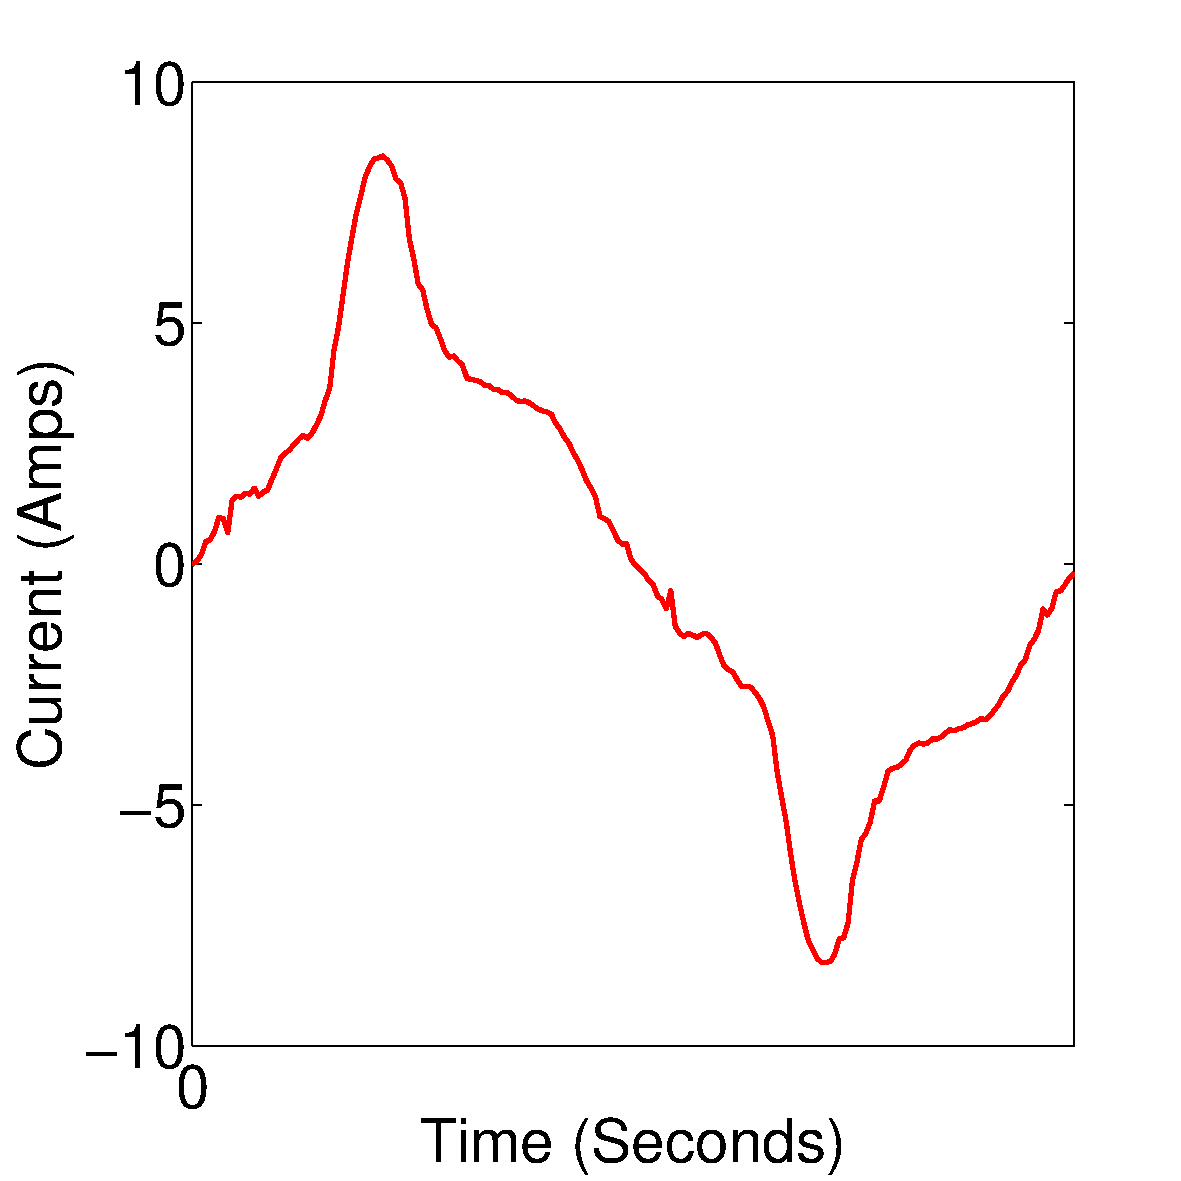
\includegraphics[width=0.4\textwidth,height=0.3\textheight]{figs/Circuit4TransientSingle.pdf} \hspace{1em}&
    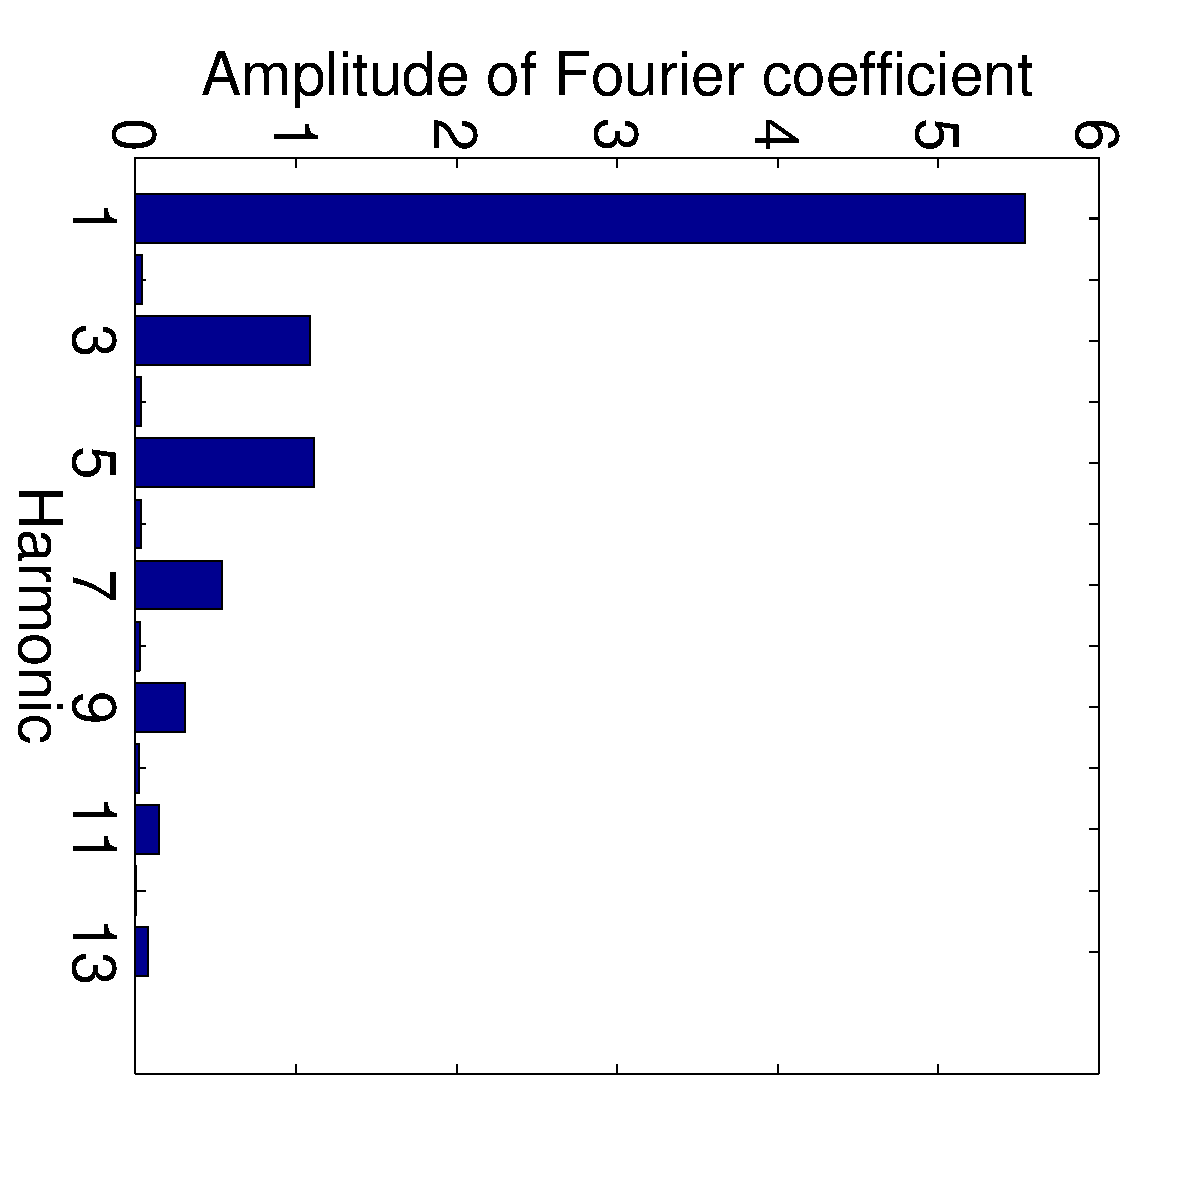
\includegraphics[width=0.4\textwidth,height=0.3\textheight,angle=90]{figs/circuit4TransientFFT.pdf} \tabularnewline
    (a) & (b)\tabularnewline
    \end{tabular}
    }
	\caption{Circuit 4 (a) Current Waveform and (b) Harmonics.}
	\label{fig_harmonicsexample}
\end{figure*}

%\begin{figure}[ht]
%\centering
%\includegraphics[width=3.2in]{figs/harmonicsexample.pdf}
%\caption{Harmonics (courtesy: \cite{eebook}).}
%\label{fig_harmonicsexample}
%\end{figure}
\begin{figure*}[h]
	\centering{
    \begin{tabular}{cc}	
	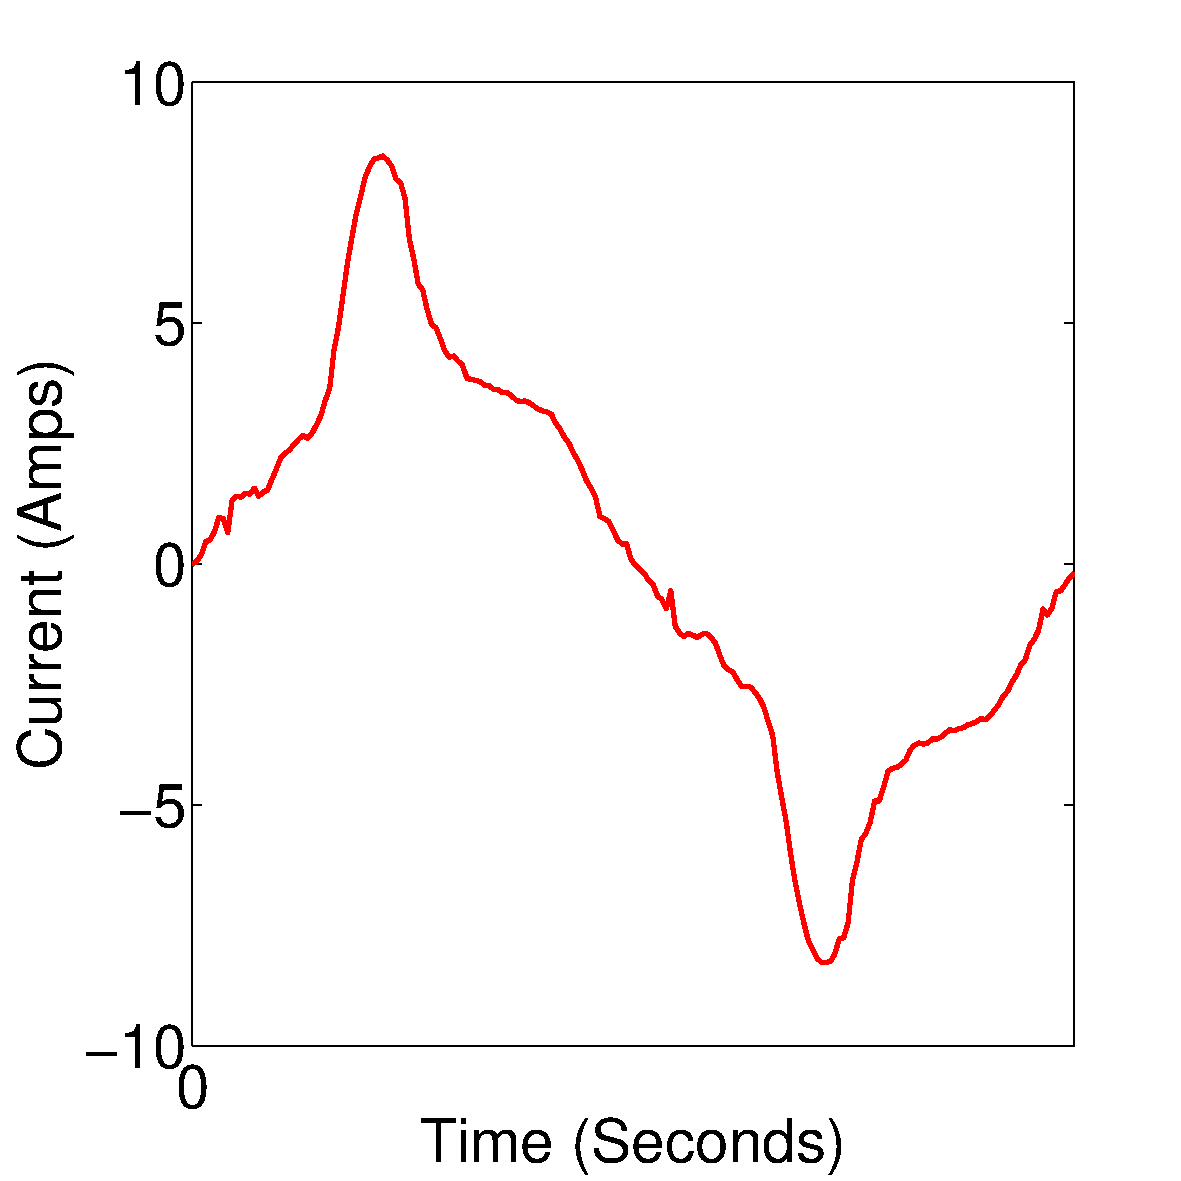
\includegraphics[width=0.4\textwidth,height=0.3\textheight]{figs/Circuit4TransientSingle.pdf} \hspace{1em}&
    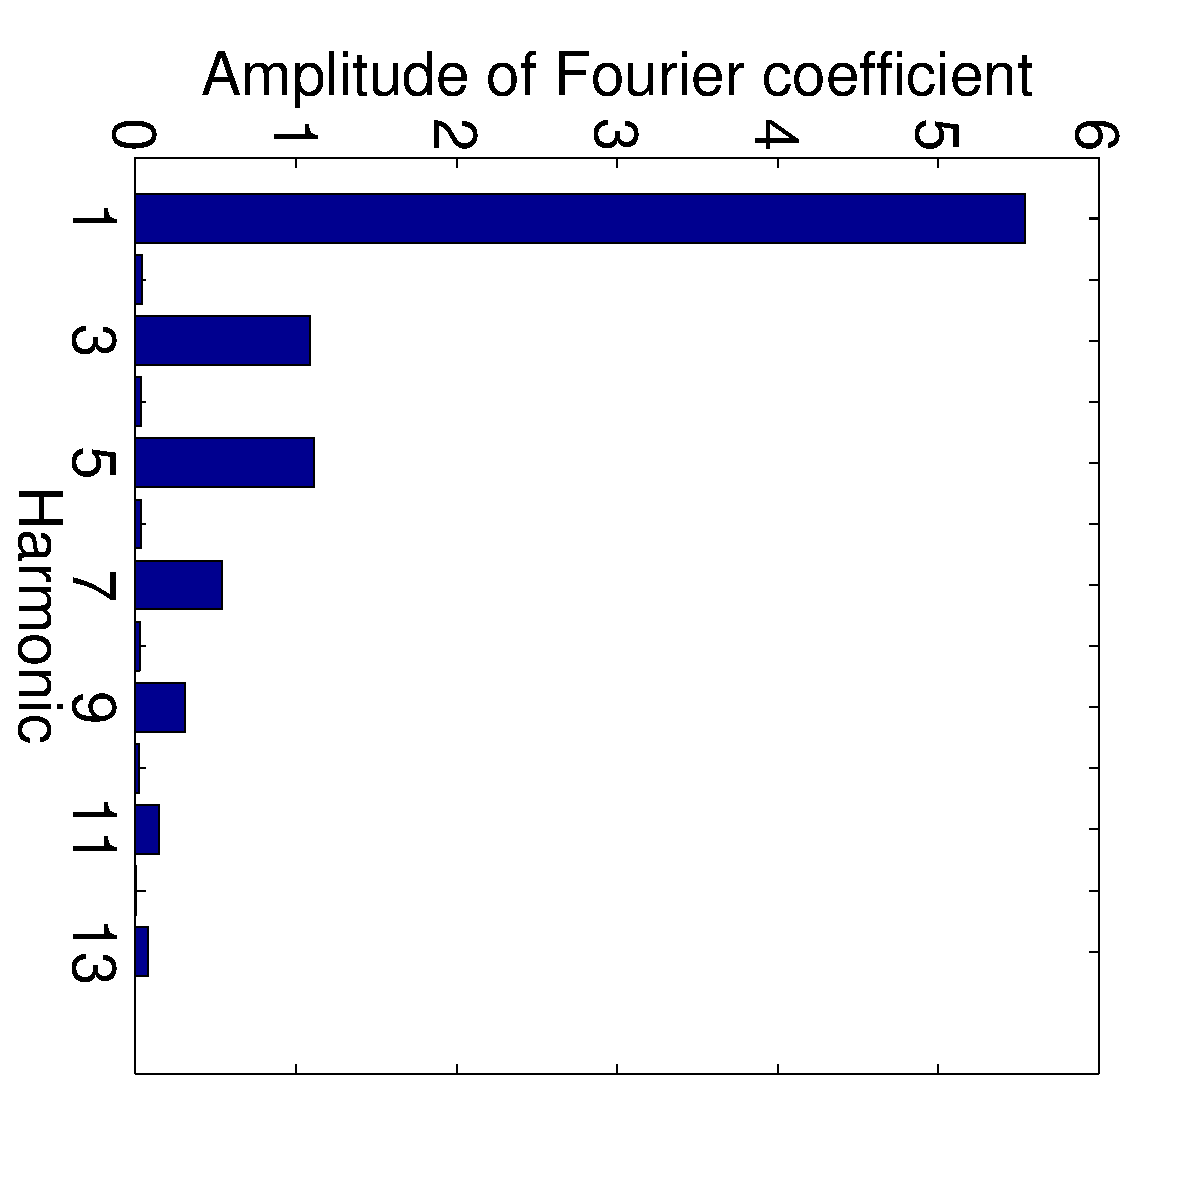
\includegraphics[width=0.4\textwidth,height=0.3\textheight,angle=90]{figs/circuit4TransientFFT.pdf} \tabularnewline
    (a) & (b)\tabularnewline
    \end{tabular}
    }
	\caption{Circuit 4 (a) Current Waveform and (b) Harmonics.}
	\label{fig_harmonicsexample}
\end{figure*}

This (or any) type of waveform can be expressed as a Fourier series.
Consider a periodic waveform $x(t) = x(t+T_0)$,
%\begin{equation}
%\label{eq_fourier}
%x(t) = x(t+T_0)
%\end{equation}
where $T_0$ is the period.
$x(t)$ can be
rewritten as
\begin{equation}
x(t) = \sum_{n=0}^{\infty}A_n cos(\frac{2\pi nt}{T}+\theta_n)
\end{equation}
where $\omega = \frac{2\pi}{T} = 2\pi f$,
$A_n$ denote the amplitudes and $\theta_n$ denote the phases.
Here $\omega$ is the fundamental frequency;
the integer multiples of basic frequencies $2\omega$, $3\omega$,
and so on are referred to as {\it harmonics}.
Figure~\ref{fig_harmonicsexample} (b) 
depicts a Fourier spectrum of
the current waveform of Figure~\ref{fig_harmonicsexample} (a).
The x-axis is the ordered harmonics and
y-axis shows the amplitude of harmonics.
%To identify electrical harmonics,
%we usually study
%harmonics in the odd number, e.g.
Typically, odd harmonics are of interest, e.g.,
3rd harmonic, 5th harmonic, and so on.



%%%%%%%%%%%%%%%%%%%%%%%%%%%%%%%%%%%%%%%%%%%%%%%%%%%%%%%%%%%%%%%%%%

%\subsubsection{Three Typical Types of Devices}
%Generally there are three types of devices or loads,
%namely electrothermal devices, electromechanical devices
%and  power electronic devices.
%In this part, we will focus on the transient states of
%different kinds of devices.

%Electrothermal devices include incandescent lamp and
%fluorescent lamp.
%Figure\ref{fig_incadescentLamp} shows
%the transient changes of an incandescent lamp.
%The x-axis is time in unit of seconds and y-axis
%is apparent power.
%After around ten cycles, the incandescent lamp
%goes to a steady state.
%\begin{figure}[ht]
\centering
\includegraphics[width=3in]{figs/incandescentLamp.pdf}
\caption{Incandescent Lamp Transient (courtesy: \cite{leeb1993PhdThesis}).}
\label{fig_incadescentLamp}
\end{figure}


%Electromechanical loads includes direct current machines,
%induction machines
%and synchronous machines.
%The starting characteristic of motor is depicted
%in Figure\ref{fig_inductortransient}.
%The starting duration of this induction machine lasts
%for around 0.8 seconds.
%In the first 0.4 seconds, the power of this device consumes
%vibrates frequently.
%Then it goes to a relatively steady state in the second 0.4 seconds.
%\begin{figure}[ht]
%\centering
%\includegraphics[width=3in]{figs/inductortransient.pdf}
%\caption{Induction Motor Transient (courtesy: \cite{leeb1993PhdThesis}).}
%\label{fig_inductortransient}
%\end{figure}

%Electronic devices are widely used in home and office nowadays,
%such as PC, monitor, printer and so on.
%Figure\ref{fig_pctransient} depicts the generated harmonics
%when a computer starts up.
%X-axis represents time and Y-axis denotes current.
%In the first 0.12s, the harmonics changes, after that
%the PC goes to a stable state.
%\begin{figure}[ht]
%\centering
%\includegraphics[width=3in]{figs/pctransient.pdf}
%\caption{Personal Computer Transient States (courtesy: \cite{leeb1993PhdThesis}).}
%\label{fig_pctransient}
%\end{figure}

%In addition, we introduce a special device Variable Speed Devices(VSDs).
%In commercial or industrial buildings,
%VSDs are often installed to optimize the energy consumption
%and controllability.
%Now we overview the inside system of VSD to better
%understand it.
%A typical VSD is composed of a rectifier, a dc-bus link,
%an inverter and an induction motor as Figure\ref{fig_VSDsystem}
%\begin{figure}[ht]
%\centering
%\includegraphics[width=3 in]{figs/VSDsystem.png}
%\caption{Topology and typical circuit model of variable speed drive (Courtesy:\cite{lee2003PhdThesis}).}
%\label{fig_VSDsystem}
%\end{figure}
%In the front end, 60Hz alternating current inputs into the rectifier,
%in which rich harmonics are created. Then power is converted to
%DC bus then re-converted to alternating current by inverter. 

%The VSD device generate power variably instead of at a
%discrete state. For instance, it may produce power ranging from
%$100w$ to $200w$. 
%Therefore they cannot be distinguished by simply ON/OFF steady states 
%because the power changes during OFF is not the oppose value during ON.


%\section{Defining disaggregation}
\section{Formalisms}
\label{sec:problem}

%Different research efforts define the problem of energy disaggregation
%in different ways.

Since Hart first defined the problem of energy disaggregation~\cite{hart1992}, its
exact definition has varied slightly. To make the problem more tractable and to
tailor it to specific use cases, researchers have made varying assumptions
about what information is given.
The bare bones version of disaggregation, as originally proposed
by Hart~\cite{hart1992}, assumes that only
aggregated current and voltage data is available as features. Other
researchers assume additional information is known, such as, 
the total number of devices\footnote{Disaggregation can only be meaningfully
  performed for devices/appliances whose power consumption is over a minimal
  threshold, typically 50 to 200 W. The number of devices here refer to those above this
  threshold.}, the number of steady power consumption states of 
devices and their corresponding power levels, and non AC power features. 
There are thus numerous formulations of the energy disaggregation problem and
these distinctions need to be considered while performances of
algorithms are compared. 
Broadly, the disaggregation problem can be solved in supervised,
unsupervised, or semi-supervised settings.

%\subsection{Definition of Supervised Energy Disaggregation}
In supervised learning approaches, labeled data is available for a period of
time, i.e., the on/off state of each device is known. 
For instance, \cite{liang2010load} assume that all devices are known
and formulate the objective function as one of 
minimizing error between the disaggregated devices and 
the corresponding ground truth devices. 
In~\cite{kolter2012aistat} it is
assumed that the power levels of individual devices are known. 
The problem then is to find the on/off events
for different devices over a period of time.
The input to supervised learning methods is thus training data consisting of
aggregated power and non-power features over time T, and each device's power
consumption over T.
Once a model is trained, given new data over
time T', the output is the disaggregated power for each device over T'.
In addition to 
power related features such as current, voltage, 
or the non-powers features such as time of day, day of week, month season,
weather information, may be given. 

\iffalse
Unsupervised or semi-supervised energy disaggregation is a harder problem since 
labeled data is not available, including any information regarding power
levels of devices. Some researchers assume the
number of devices or circuits (see Section x for details) are
known~\cite{kim2010unsupervised,kolter2012aistat,parson2012nonintrusive,johnson2012bayesian,shao2013temporal}.
\manishc{can you add a few more refs to this}
\huijuanc{change as following paragraph}.
This information can typically be found from circuit wiring diagrams.
Others assume no
such information, e.g.,~\cite{gonccalves2011unsupervised}
and~\cite{wytock2014contextually}, 
\manishc{is the accuracy of these methods (which assume no information at all
  low? Here you want to provide a high level comparison between the
  unsupervised/supervised approaches} \huijuanc{agree. The follows is the revised paragraph}
 \fi 
Unsupervised or semi-supervised energy disaggregation is a harder problem because, 
comparing to supervised learning approaches, the only known information is the aggregated 
data. 
The number of devices/circuits or the characteristics of each device, 
such as power levels are either unknown~\cite{gonccalves2011unsupervised,wytock2014contextually}
or assumed by the researchers to be fixed~\cite{kim2011unsupervised,kolter2012aistat,parson2012nonintrusive,johnson2012bayesian,shao2013temporal}.  
In spite of these difficulties, the
disaggregation performance of unsupervised approaches 
may approach that of supervised approaches. 
%
%In particular, it is assumed that 
%the detailed devices information is unavailable, 
%such as the number of power levels (the steady states of a device), 
% the power value of each level, and the 
%exact time when it is turned on or off. 
Note that evaluation of any method, whether supervised or unsupervised, requires that
ground truth information be available (number of devices and their on/off power states).

%In the evaluation phase, 
%even if we do not know the number of devices,
%we still need to compare the disaggregated 
%devices with the true devices. 
%Therefore we assume the number of devices is known. 

%\textit{Energy Disaggregation with Power}
%Given the aggregated power record $Y=y_1, ..., y_i, ..., y_T$
%in the unit of watts
%over a period of time $T$, 
%the ground truth of $N$ time series 
%$X_j = x_{1j}, ...x_{ij}, ... x_{Tj}, j\in[1, N]$ 
%corresponding to $N$ circuits or devices, 
%estimate disaggregated $N$ time series 
%$\hat{X_j }= \hat{x_{1j}}, ...\hat{x_{ij}}, ... \hat{x_{Tj}}, j\in[1, N]$, 
%such that 
%the L2 norm error between the disaggregated power values and 
%the ground truth is minimal as in equation \ref{eq_powerObj}.
%\begin{equation}
%\label{eq_powerObj}
%\min_{\hat{x_{ij}}} \sum_{i=1}^T (\sum_{j=1}^N \hat{x_{ij}}-y_i)^2
%\end{equation}
%For supervised learning, we know each time series, 
%then equation \ref{eq_powerObj} can be written as 
%$\min_{\hat{x_{ij}}} \sum_{i=1}^T \sum_{j=1}^N (\hat{x_{ij}} - x_{ij})^2$ 
%for L2 norm. 

\subsection{Definition}
For our purposes, we will assume the following definition of the problem:
Given an aggregate power consumption time series $Y=y_1, ..., y_T$, and a set of
power related and contextual features, $f=f_1, ..., f_T$ over a period of time T, 
the problem is to estimate the disaggregated power consumption of $M$ devices 
$\hat{X_m }= \hat{x}_{1}^{(m)}, ...\hat{x}_{t}^{(m)}, ... \hat{x}_{T}^{(m)}, m\in[1, M]$, 
such that a loss function on the sum of the power consumption of the $M$
devices and the aggregate power consumption is minimal. 
\begin{equation}
\label{eq_powerObj}
\min_{\hat{x}_{t}^{(m)}} \{ \sum_{t=1}^T \mathscr{L}_t(\sum_{m=1}^M \hat{x}_{t}^{(m)}, y_t) \}
\end{equation}
where $\mathscr{L}_t$ is the loss function between 
the sum of $M$ estimated time series at $t$, 
and $y_t$ is the ground truth aggregated power feature at time $t$. 
$\mathscr{L}$ is usually the $\mathscr{L}1$-norm $\sum_{m=1}^M |\hat{x}_{t}^{(m)} - y_t|$
or the $\mathscr{L}2$-norm $\sum_{m=1}^M (\hat{x}_{t}^{(m)}-y_t)^2$.

For supervised learning, 
the ground truth of $M$ time series 
$X_m = x_{1}^{(m)}, ...x_{t}^{(m)}, ... x_{T}^{(m)}, m\in[1, M]$ 
corresponding to $M$ circuits or devices is also given.
%Equation (\ref{eq_powerObj}) is written as 
%$\min_{\hat{x}_{t}^{(m)}} \{ \mathscr{L}_{t}^{(m)}(\sum_{t=1}^T \sum_{m=1}^M \hat{x}_{t}^{(m)}, y_t) \}$.
%\manishc{pushing the sum over T into the loss function is not correct; also y
%  still depends on t} \huijuanc{already deleted.}

%% Given a set of time series $Y=y_1, ..., y_T$, 
%% the aggregated power feature over a period of time T, 
%% and contextual features of $M$ devices; 
%% the problem is to estimate disaggregated $M$ time series 
%% $\hat{X_m }= \hat{x}_{1}^{(m)}, ...\hat{x}_{t}^{(m)}, ... \hat{x}_{T}^{(m)}, m\in[1, M]$, 
%% such that 
%% the difference between the sum of the $M$ power features and 
%% the aggregated power feature is minimal. 
%% \begin{equation}
%% \label{eq_powerObj}
%% \min_{\hat{x}_{t}^{(m)}} \{ \sum_{t=1}^T \mathscr{L}_t(\sum_{m=1}^M \hat{x}_{t}^{(m)}, y_t) \}
%% \end{equation}
%% where $\mathscr{L}_t$ is the loss function between 
%% the sum of $M$ estimated time series at $t$, 
%% and $y_t$ is the ground truth aggregated power feature at time $t$. 
%% $\mathscr{L}$ is usually $\mathscr{L}_1$ norm $|\sum_{m=1}^M \hat{x}_{t}^{(m)} - y_t|$
%% or $\mathscr{L}_2$ norm $(\sum_{m=1}^M \hat{x}_{t}^{(m)}-y_t)^2$.


%The input of the unsupervised disaggregation is 
%the aggregated power over time T, 
%and the number of devices. 
%The output is the same as that of supervised disaggregation, 
%i.e., the disaggregated power for each device over T. 
%The unsupervised energy disaggregation is defined as follows. 

%\textit{Supervised Energy Disaggregation}
%Given the aggregated power record $Y=y_1, ..., y_i, ..., y_T$
%in the unit of watts
%over a period of time $T$, 
%the ground truth of $N$ time series 
%$X_j = x_{1j}, ...x_{ij}, ... x_{Tj}, j\in[1, N]$ 
%corresponding to $N$ circuits or devices, 
%estimate disaggregated $N$ time series 
%$\hat{X_j }= \hat{x_{1j}}, ...\hat{x_{ij}}, ... \hat{x_{Tj}}, j\in[1, N]$, 
%such that 
% the error between the disaggregated power values and 
% the ground truth is minimal as in equation \ref{eq_supervisedObj}.
% \begin{equation}
% \label{eq_supervisedObj}
%\min \sum_{i=1}^T \sum_{j=1}^N (\hat{x_{ij}} - x_{ij})
%\end{equation}
%Since the sum of $y_i= \sum_{j=1}^N x_{ij}$, 
%equation \ref{eq_supervisedObj} is the same as equation \ref{eq_unsupervisedObj}.

%\subsection{Definition of Unsupervised Energy Disaggregation}
%\textit{Energy Disaggregation}
%Given the aggregated power record $Y=y_1, ..., y_i, ..., y_T$
%in the unit of watts
%over a period of time $T$, 
%the device number $N$,
%find $N$ time series$\hat{X_j }= \hat{x_{1j}}, ...\hat{x_{ij}}, ... \hat{x_{Tj}}, j\in[1, N]$ 
%corresponding to each circuit or device,
% such that
% the error between the aggregated power values and 
% sum of the disaggregated power values is minimized as equation \ref{eq_unsupervisedObj}.
% \begin{equation}
% \label{eq_unsupervisedObj}
%\min \sum_{i=1}^T (\sum_{j=1}^N \hat{x_{ij}}-y_i)
%\end{equation}

%\begin{equation}
%y_i=\sum_{j=1}^N{x_{ij}}, i\in[1, T]
%\end{equation}
%and
%\begin{equation}
%x_{ij} \approx x_{ij}^{true}
%\end{equation}
%where $x_{ij}^{true}$ is the true value of device $j$ at time $i$.
%\end{disagg}
%The objective function can be written as Equation (\ref{eq_objective}) to minimize the 
%power value error between the disaggregated values and the true value. 
%\begin{equation}
%\label{eq_objective}
%\min \sum_i\sum_j \{ x_{ij} - x_{ij}^{true}\}
%\end{equation}

\subsection{Technology Timeline}
The evolution of approaches to energy disaggregation is summarized in Figure~\ref{fig_timeline}.  
The algorithms for this problem  have developed through several stages by incorporating 
features of increasing levels of sophistication. 
In the early stages of disaggregation research, algorithms were based
on the features of real and reactive power, transient startup of current or power, and 
harmonics. In the next stage of development, algorithms were based on wavelet
transforms of current, 
duration time of specific steady state of real power, the waveform of current or voltage, 
and current/voltage noise. 
\iffalse
\huijuanc{comment out until huijuan's next comments}
In the current stage of development, algorithms use electromagnetic
 interference (EMI), eigenvalues of current, and devices correlation.
 \huijuanc{comment out}
\manishc{the above needs to be rewritten; e.g., it is not that everybody uses
  EMI for disaggregation now; write it as people have been trying different
  features - the ones used recently say EMI are not necessarily better, nor
  are most people using them. They are just novel, and good results were
  reported, but there may be other reasons like having to install sensors etc that
  everbody may not adopt them.} \huijuanc{the last sentence of this paragraph is rewritten as follows.}
  \fi
In recent studies, algorithms have used eigenvalues of current, and
device correlation information. As researchers explore new features to use
for disaggregation, we must keep in mind that good results are not necessarily
the only yardstick but ease of instrumenting sensors to capture such features
is also a key objective.

\iffalse
An evolution of approaches to 
energy disaggregation 
is summarized in Figure~\ref{fig_timeline}.
On the one hand, 
features are explored continuously. 
On the other hand, 
algorithms based on these features 
develops through several stages. 
In the first stage of development, 
feature exploration of electrical devices has been developing 
from the real and reactive power,
transient startup of current or power, harmonics. 
The next stage of development is 
the wavelet of current, duration time of specific steady state
of real power, the waveform of current or voltage, and current/voltage noise. 
After these techniques, 
electromagnetic interference (EMI),
eigenvalues of current and devices correlation are 
recently used.
\fi

\begin{figure}[ht]
\centering
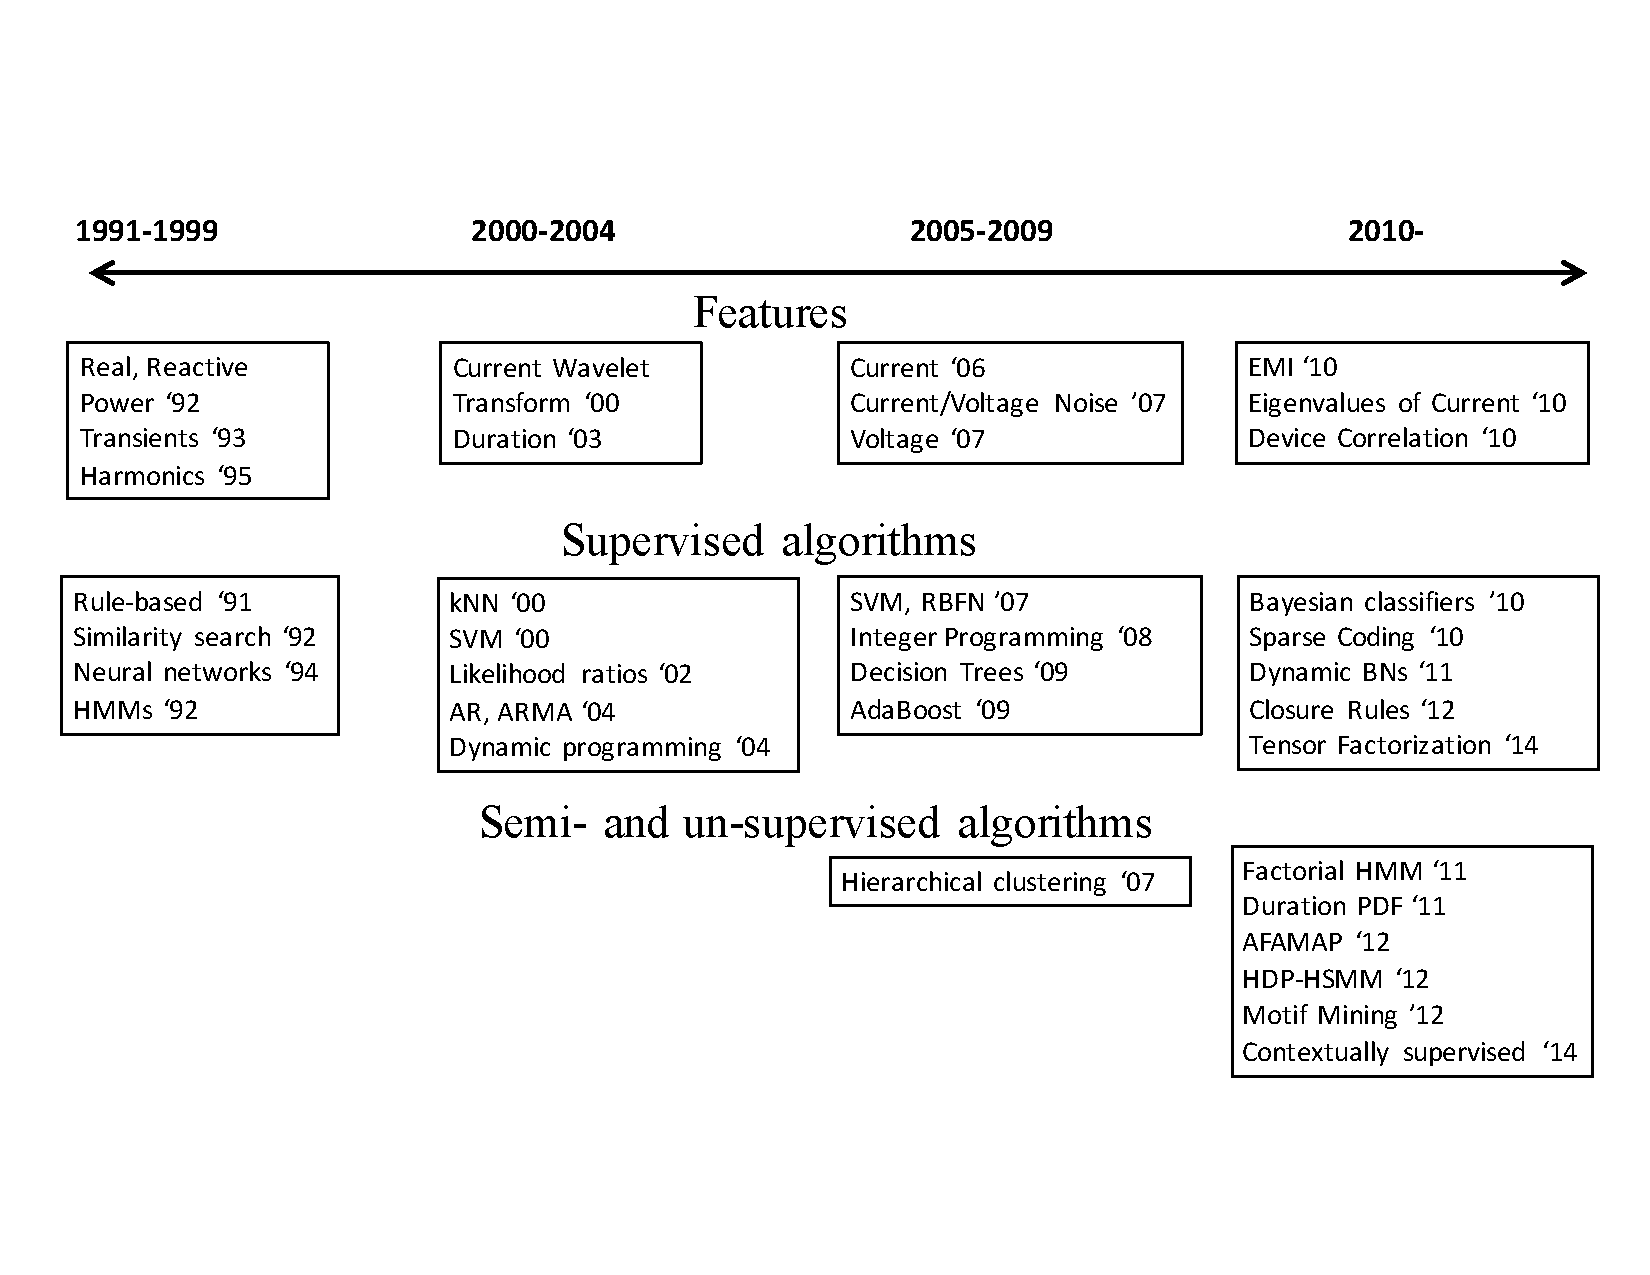
\includegraphics[width=5in]{figs/algo-timeline.pdf}
\caption{Timeline of features and algorithms proposed for energy disaggregation.}
\label{fig_timeline}
\end{figure}

Concomitantly,
algorithms adopted in this area have experienced an accelerating progress;
from supervised learning algorithms, including optimization algorithms 
and statistical models; 
to unsupervised learning and semi-supervised learning 
(see Fig.~\ref{fig_timeline}).
Supervised learning employs each circuit/device's data
as training data, which is laborious to collect.
%\manishc{what are the green ones?}\huijuanc{add the green ones' explanation.}
They include rule-based approaches; pair-wise matching
and neural  networks which were proposed in 1990s;
k-nearest neighbor algorithms (kNN); support vector machines (SVM) and kernel based
subspace classification (KSC); general likelihood ratio-based methods;
auto-regression and moving average methods; 
radial basis function network methods (RBFN);
decision trees; adaBoost; Bayesian classifiers;
space coding; dynamic Bayesian networks; closure rules;
Viterbi algorithms; dynamic programming, integer programming, 
and nonnegative tensor factorization.
%Also, the algorithm which is often employed in
%information processing area, wavelet transform,
%was used in 2000~\cite{chan2000harmonics}.
Since 2006, unsupervised and semi-supervised algorithms
have become the preferred approach to identify devices.
These include hierarchical clustering,
factorial HMMs, 
approximate factorial additive MAP (AFAMAP),
difference FHMM which adds prior knowledge of the device, 
hierarchical Dirichlet process hidden semi-Markov models,
motif mining, and contextually supervised source separation. 
In the next two sections, we explain the features and the algorithms in detail.





%\section{Identifying Devices by Features}
\section{Disaggregation Features}
\label{sec:features}
%Previous surveys have summarized the features for energy disaggregation, primarily from an
%electrical engineering viewpoint [\citeNP{zeifman2011nonintrusive,lee2004exploration,
%liang2010load,zoha2012survey}].
%We target this survey for the data mining community and complement prior literature 
%by providing details of existing features and newer ones, and 
%summarizing the strengths and weaknesses of these features in disaggregation.
%and add the computational cost of each approach. 
%

%\manishc{like we discussed, focus this section on features, and move data
%  collection to later}
%\huijuanc{ok. already moved.}
In this section we briefly outline several features that are used in disaggregation and
classify them based on different types like AC vs. non-AC or steady vs. transient state. 
%Data collection methods and instrumentation used 
%We also present techniques and methodologies by which the data is collected to assist feature
%extraction for the learning algorithms. 
%%\section{Experiments Setup and Data Sets}
\subsection{Data Collection  and Public Data Sets}
\label{sec:setup}
The usefulness of energy disaggregation algorithms is a function of the aggregated datasets' 
availability. 
Therefore we need to collect this data by installing the corresponding meters and 
sensors and setting up the necessary experiments. 

\subsubsection{Meters}
Generally speaking,
there are two types of data that can be used to disaggregate devices:
AC power information and non-AC power information.
To obtain AC power data, a real power meter, reactive power meter,
ammeter, and voltage meter (usually consolidated into one meter) can be installed to
record different power values, current or voltage values, 
and noise generated by power line.  
Sensors are installed to collect non-AC power data, like electromagnetic fields (EMF) 
around devices~\cite{giri_study_2012}, light, and sound~\cite{kim2009viridiscope}.

Figure~\ref{fig_metersConnection} illustrates how
four types of meters/sensors are installed in a building.
After two-phase power is delivered into the home, %\manishc{usually homes have 2-phase},
three power meters, which record real power,
current, and voltage are installed on
these three entry power lines separately. 
A power meter is installed on each circuit, such as for the refrigerator,
 to monitor the
true status of the devices (to validate results).
A sensor is plugged into the outlet to monitor the
voltage noise data.
Besides these AC-power meters,
an electromagnetic field sensor, 
a sound sensor , and a light sensor
may also be installed around devices,
such as the refrigerator, to capture its electrical magnetic field, 
sound-related, and light-related operations.

\begin{figure}[ht]
\centering
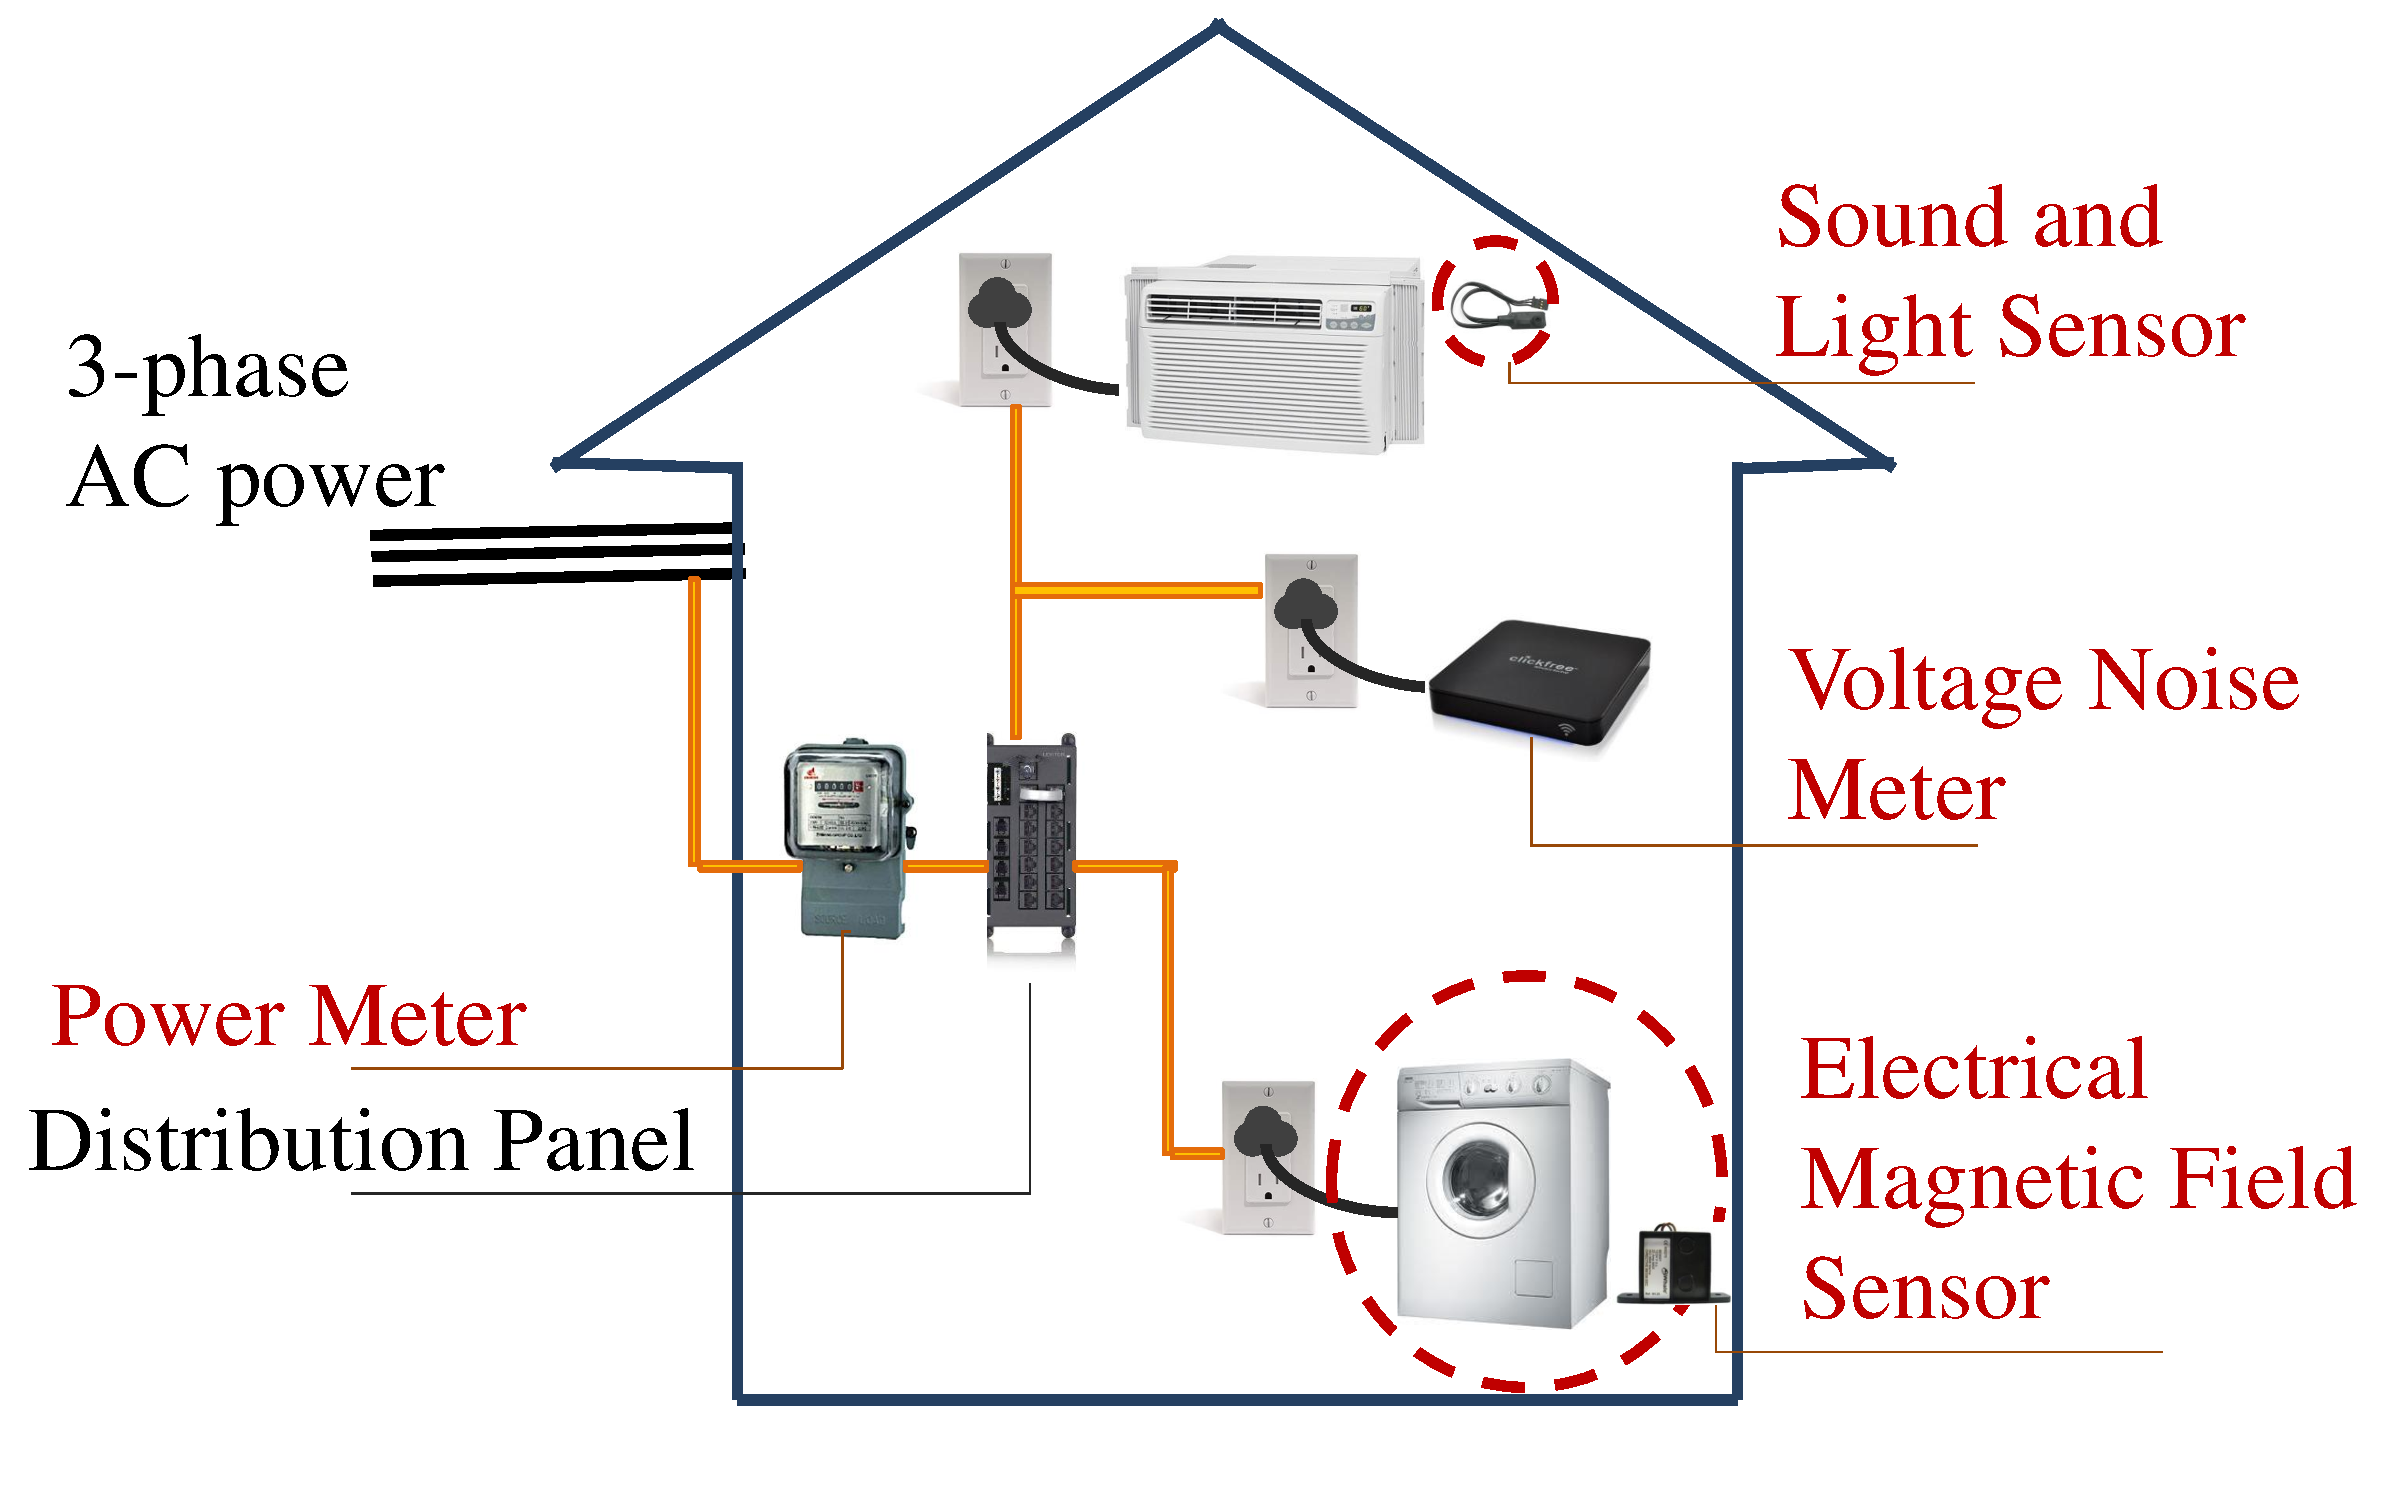
\includegraphics[width=3 in]{figs/metersConnection.pdf}
\caption{Four Types of Meters in a Building.}
\label{fig_metersConnection}
\end{figure}

\begin{table}
\caption{Meters Used in Experiments.}
\small
\label{tab_meters}
\begin{center}
\makebox{
\begin{tabular} {|l|l|l|l|}
\hline
Meter Types & Meter Name & Meter Example & Recorded Features \\
\hline
\multirow{4}{*}{AC power} & ammeter & TED, LEM LA55-P~\cite{meterTED} & AC waveform, harmonics \\
\cline{2-4}
& voltage meter & Pico TA041~\cite{meterPico}& voltage waveform, voltage \\
\cline{2-4}
& real power meter & National Instruments USB-9215A~\cite{meterNI} & real power \\
\cline{2-4}
& reactive power meter & TrendPoints EnerSure~\cite{meterTrend}& reactive power \\
\cline{2-4}
& voltage noise meter & Build by author & voltage noise \\
\hline
\multirow{3}{*}{Non-AC power} & electromagnetic field meter & Trifield~\cite{meterEMF}&electromagnetic field \\
\cline{2-4}
& sound sensor& mindstorms~\cite{meterSound}& sound strongness \\
\cline{2-4}
& light sensor & extech~\cite{meterLight}& light strongness \\
\cline{2-4}
& temperature meter & amprobe~\cite{meterTemp}& temperature\\
\hline
\end{tabular}}
\end{center}
\end{table}


The meters or sensors that have been used in the experiments
are listed in Table~\ref{tab_meters}. 
%\manishc{can you add references for all the 'meter example' in the table} \huijuanc{done.}
Devices like an ammeter to gauge the current value, a voltage meter to record the voltage,
a wattmeter to log the real power, and a reactive power meter to record the reactive values 
are easily available.

%Regardless of whether the algorithm uses supervised or unsupervised learning, 
%both the whole-house voltage-current and individual meters for circuit/devices are needed. 
%The circuit level data, that is the ground truth, is necessary for evaluation. 

\subsubsection{Low-frequency data and high-frequency data}
%Watt meter combines ammeter with voltage meter
%and measures the real power,
%which is the product of root-mean-square(RMS)
%values of voltage and current.
%%\cite{berges2008training} describes how to record these data.
%%%Therefore ,
%%%\begin{equation}
%%%x_{rms}= \sqrt{\frac{1}{T}\int_{0}^{T}x^2(t^{'})dt^{'}}
%%%\end{equation}
%%%here $x(t)$ is the sinusoidal voltage or current as a function of $t$.
%%Also, there is reactive power meter.
%%These meters can be installed on each phase or
%%circuit to monitor the current, voltage values just as Figure\ref{fig_meters}
%%\begin{figure}[ht]
%%\centering
%%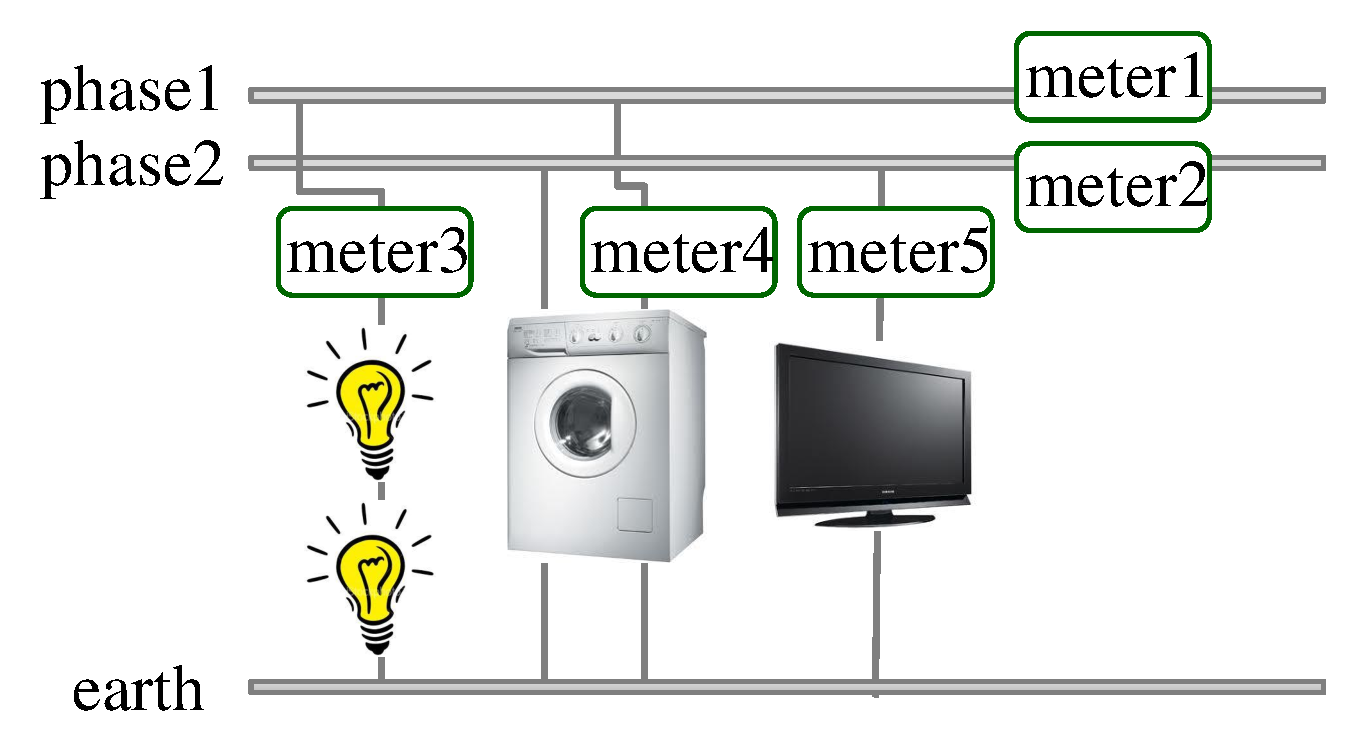
\includegraphics[width=2.5in]{figs/meters.pdf}
%%\caption{Meters on Phases and Circuits}
%%\label{fig_meters}
%%\end{figure}
%For each phase or circuit, meters can be installed
%to record the voltage or current value by voltage
%meter and ammeter.
%Real power is measured by wattmeter.

When meters are installed to monitor the voltage and current,
generally two kinds of data are collected:
low-frequency data and high-frequency data.

In North America, the basic frequency of voltage or current is
60 Hz. 
If the interval between successive data points is larger than 1/60s, 
the data recorded by the meter is low-frequency data; otherwise it is 
high-frequency data. 
High-frequency data can recover the waveform, as
illustrated in Figure~\ref{fig_threephase}.
In practice, only the apparent power
or real power is measured for low-frequency data.
For high-frequency data,
normally current and voltage are monitored separately to facilitate the capture of different device characteristics.
To capture high-order harmonics, the sampling frequency used to record the data
should be at least twice as much as the highest frequency.
When targeting to capture harmonics with the highest order $N_{highest}$, 
 the desired harmonics frequency is $N_{highest} \times 60 Hz$,
then the sampling frequency of recorded data $f$ should
meet the criteria $f \geq N_{highest} \times 1/60 Hz$. 
%\manishc{needs to be fixed} \huijuanc{done.}
%For instance, if the $11th$ harmonics is the highest order 
%we want to use, the recording frequency should be larger than $660$ Hz,
%or $1/660$s.

There are many meters that can record the low-frequency power.
However, high-frequency data must be monitored by special devices such as a TED~\cite{meterTED}.
%\manishc{provide ref.}\huijuanc{done.}
Some examples of aggregated energy data collection include
~\cite{berges2010enhancing}, where a voltage/current meter is installed in a residential
home in Pittsburgh, PA.
This experiment chooses 17 on-off devices and installs plug-level meters for
these 17 devices. 
The data is recorded at a high frequency
(100 kHz). Then features such as real and reactive power and harmonics
are extracted at the frequency of 20 Hz.
Voltage noise data~\cite{patel2007flick} is obtained 
at a high-frequency sampling rate by
plugging the meters into an outlet. Reference~\cite{baranski2003nonintrusive} installs an
optical sensor 
%\manishc{what's an optimal sensor?}\huijuanc{optical other than optimal} 
to collect the real power. Then the on-off events are extracted 
from the real power.
A detailed comparison of
a whole-house meter, circuit meters and plug-meters 
is given in~\cite{berges2010enhancing}.


%\cite{froehlich2011disaggregated} lists what frequency are needed for
%each kind of features as Figure\ref{fig_setup_froehlich2011disaggregated}.
%http://www.theenergydetective.com/how-does-ted-work
%No matter the voltage or current is recorded
%in high frequency or low frequency,
%the instantaneous values are recorded.
%Therefore the steady states,
%which corresponds to power levels
%conform to Gaussian distribution.
%More concisely, if there's average
%value of a power level $\mu$ and
%$\mu=V_{\mu}$, then
%\begin{displaymath}
%(1-\sqrt2\times V_\mu)\leq \mu \leq (1+\sqrt2)\times V_\mu
%\end{displaymath}
%
%To test whether energy disaggregation succeeds or not,
%proper data needs to be obtained.
%Some datasets are obtained by simulation in experiments.
%But majority of devices are gathered by setting
%experiments.
%Table \ref{tb_setup} lists the devices,
%recorded frequency, extracted features for each paper.

%\begin{figure}[ht]
%\centering
%\includegraphics[width=3 in]{figs/noiseflicker.png}
%\caption{Our prototype system consists of a power line noise analyzer plugged in to an ordinary
%wall outlet and connected to a PC (Courtesy:\cite{patel2007flick}).}
%\label{fig_noiseflicker}
%\end{figure}
%
%\subsubsection{EMI}
%\begin{figure}[ht]
%\centering
%\includegraphics[width=3 in]{figs/installationElectriSense.png}
%\caption{Block diagram of major components of ElectriSense (Courtesy:\cite{gupta2010electrisense}).}
%\label{fig_installationElectriSense}
%\end{figure}

\subsubsection{Public datasets}
Although there are many data sets available for energy disaggregation, 
especially in the power industry, 
the majority of them are not open to the public. 
So far there are a few public data sets, including REDD~\cite{kolter2010redd},
BLUED~\cite{anderson2012blued}, Smart~\cite{barker2012smart}, 
AMPds~\cite{makonin2013ampds}, CASAS~\cite{cook2013CASAS}, iAWE~\cite{batra2013different}, 
and GREEND~\cite{monacchi2014greend}. %(? compare more according to GREEND papers)
The first open data set REDD, when introduced, opened the doors for several 
researchers to attack the energy disaggregation problem.

So far, a majority of this data is stored as plain text. 
Some work proposes to store these datasets in a database~\cite{lai2012database}  
or builds a metadata as a standard~\cite{kelly2014metadata}. 


%\subsection{Features Summary}
%To disaggregate devices from aggregated current, voltage, or power data,
%we need to first understand the basic features of electrical devices.
We introduced
some of these features in Section~\ref{sec:basic} such as voltage, current, real power, 
reactive power, harmonics generated by current and voltage. Some more basic and 
derived features
include: startup of current; waveform of current;
wavelet of current waveform; eigenvalue of current waveform;
voltage waveform; voltage noise; EMI
by gauging noise; electromagnetic field around the devices; 
duration time of power levels by calculating current and voltage; 
and time correlation of devices. 

%The features that can be extracted from a data set 
%depend on the installed meters 
%and the sampling frequency of data recording. 
%Current meter and voltage meter can show current and voltage values
%at the sampling points.
%If the sampling frequency is high enough, larger than several hundreds Hz,
%the waveform of current or voltage can be reconstructed.
%The noise data is recorded by a special plug-in meter, which is installed in some power 
%outlets instead of being installed on main service current or voltage electrical lines.

%combination of two
%\begin{figure}[h]
%\centering
%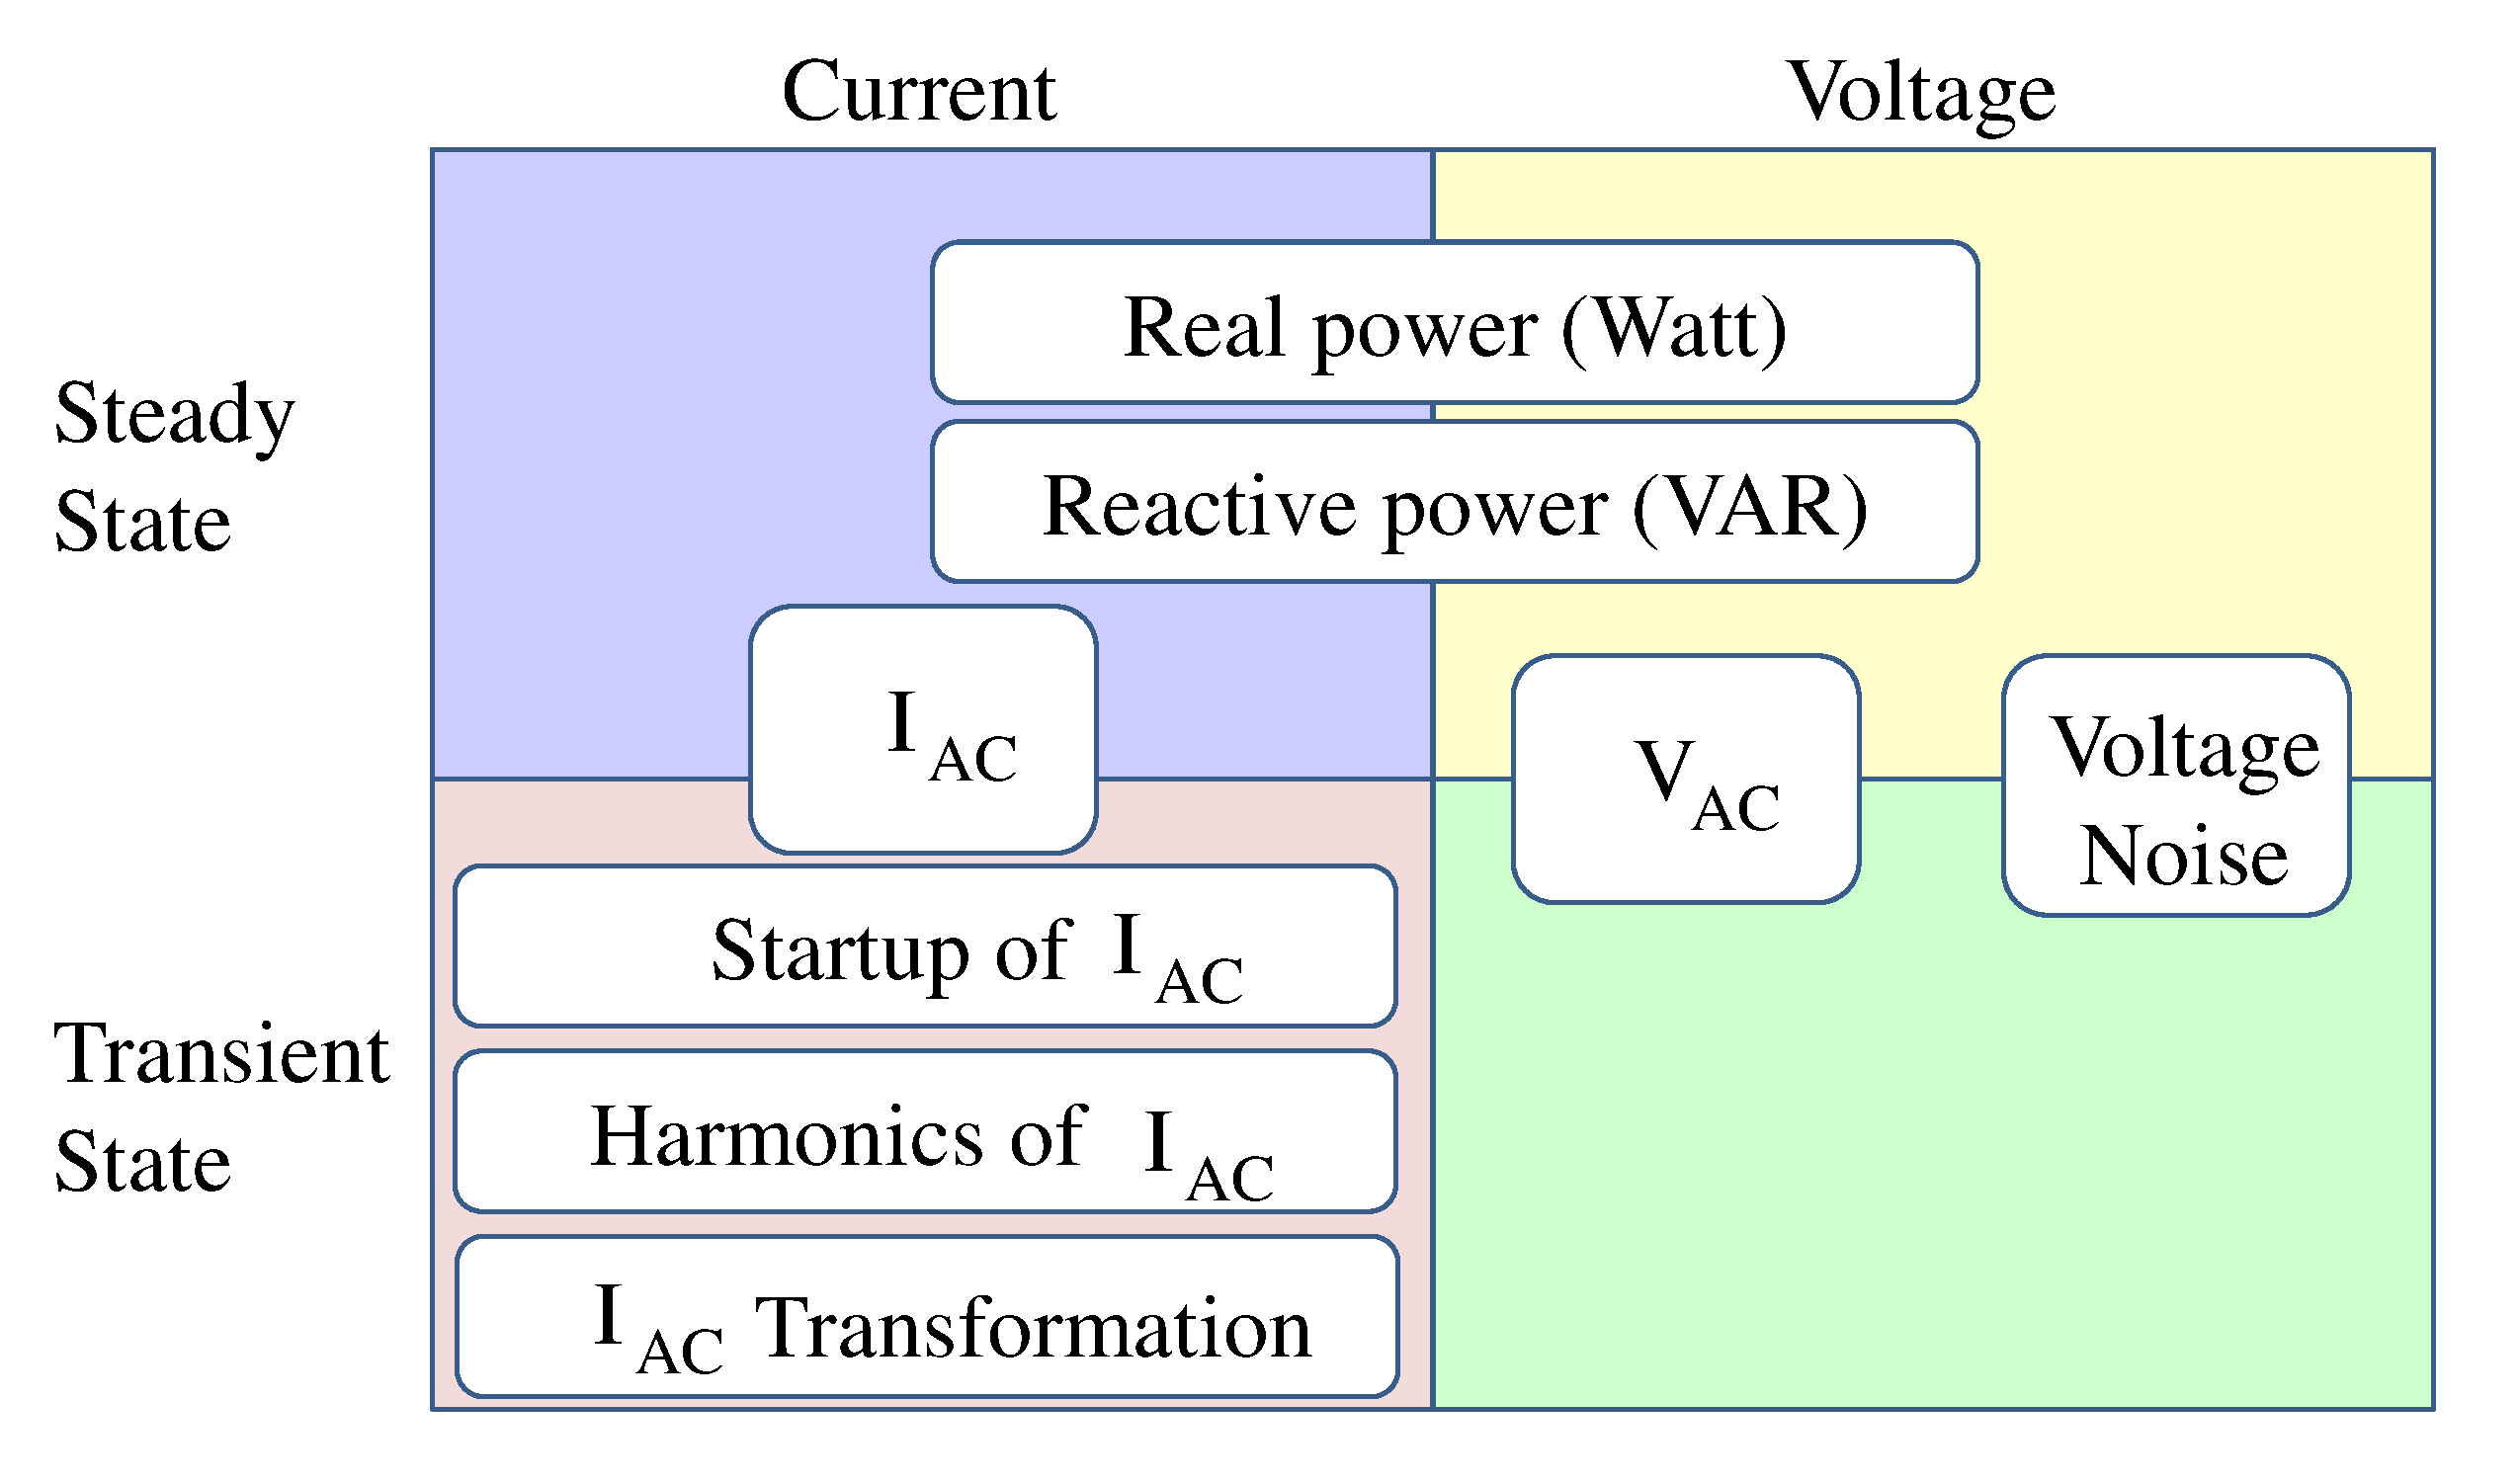
\includegraphics[width=3 in]{figs/fig_acpower.pdf}
%\caption{Category of AC Power Features}
%\label{fig_ACPowerFeatures}
%\end{figure}

%\begin{figure}[h]
%\centering
%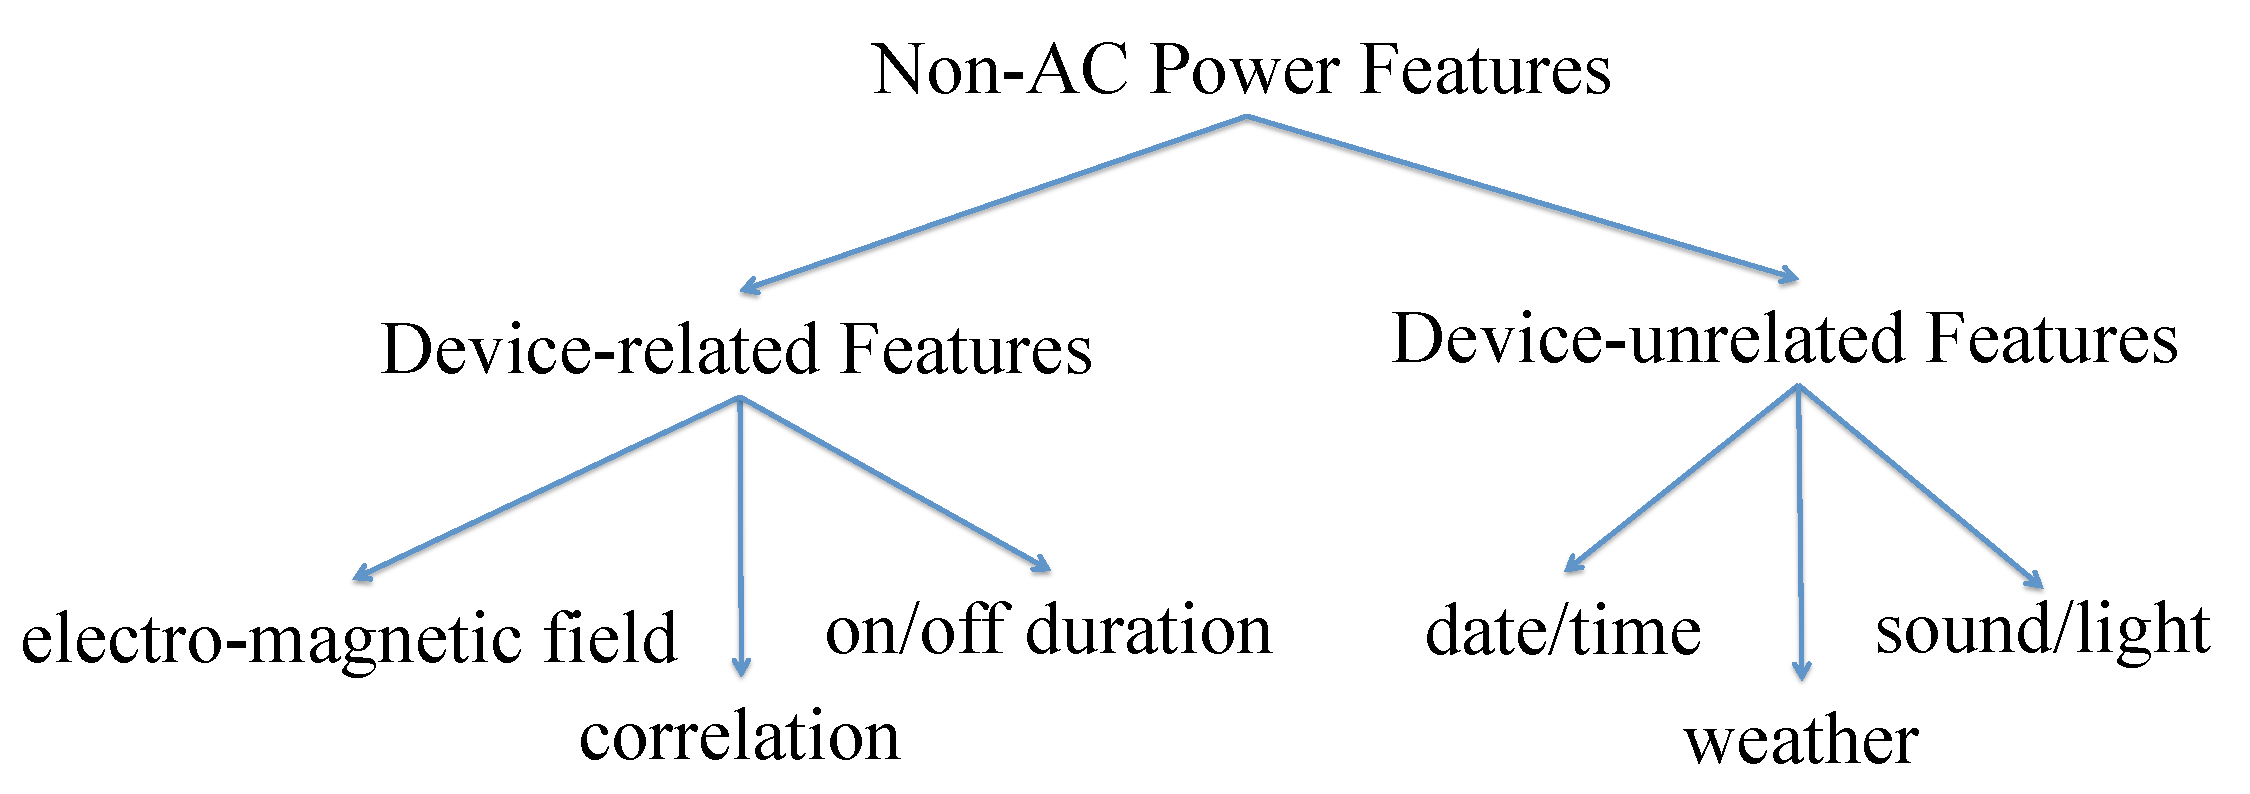
\includegraphics[width=3.5in]{figs/NonPowerFeatures.pdf}
%\caption{Category of AC Power Features}
%\label{fig_NonACPowerFeatures}
%\end{figure}

\begin{figure*}[h]
	\centering{
    \begin{tabular}{cc}
    	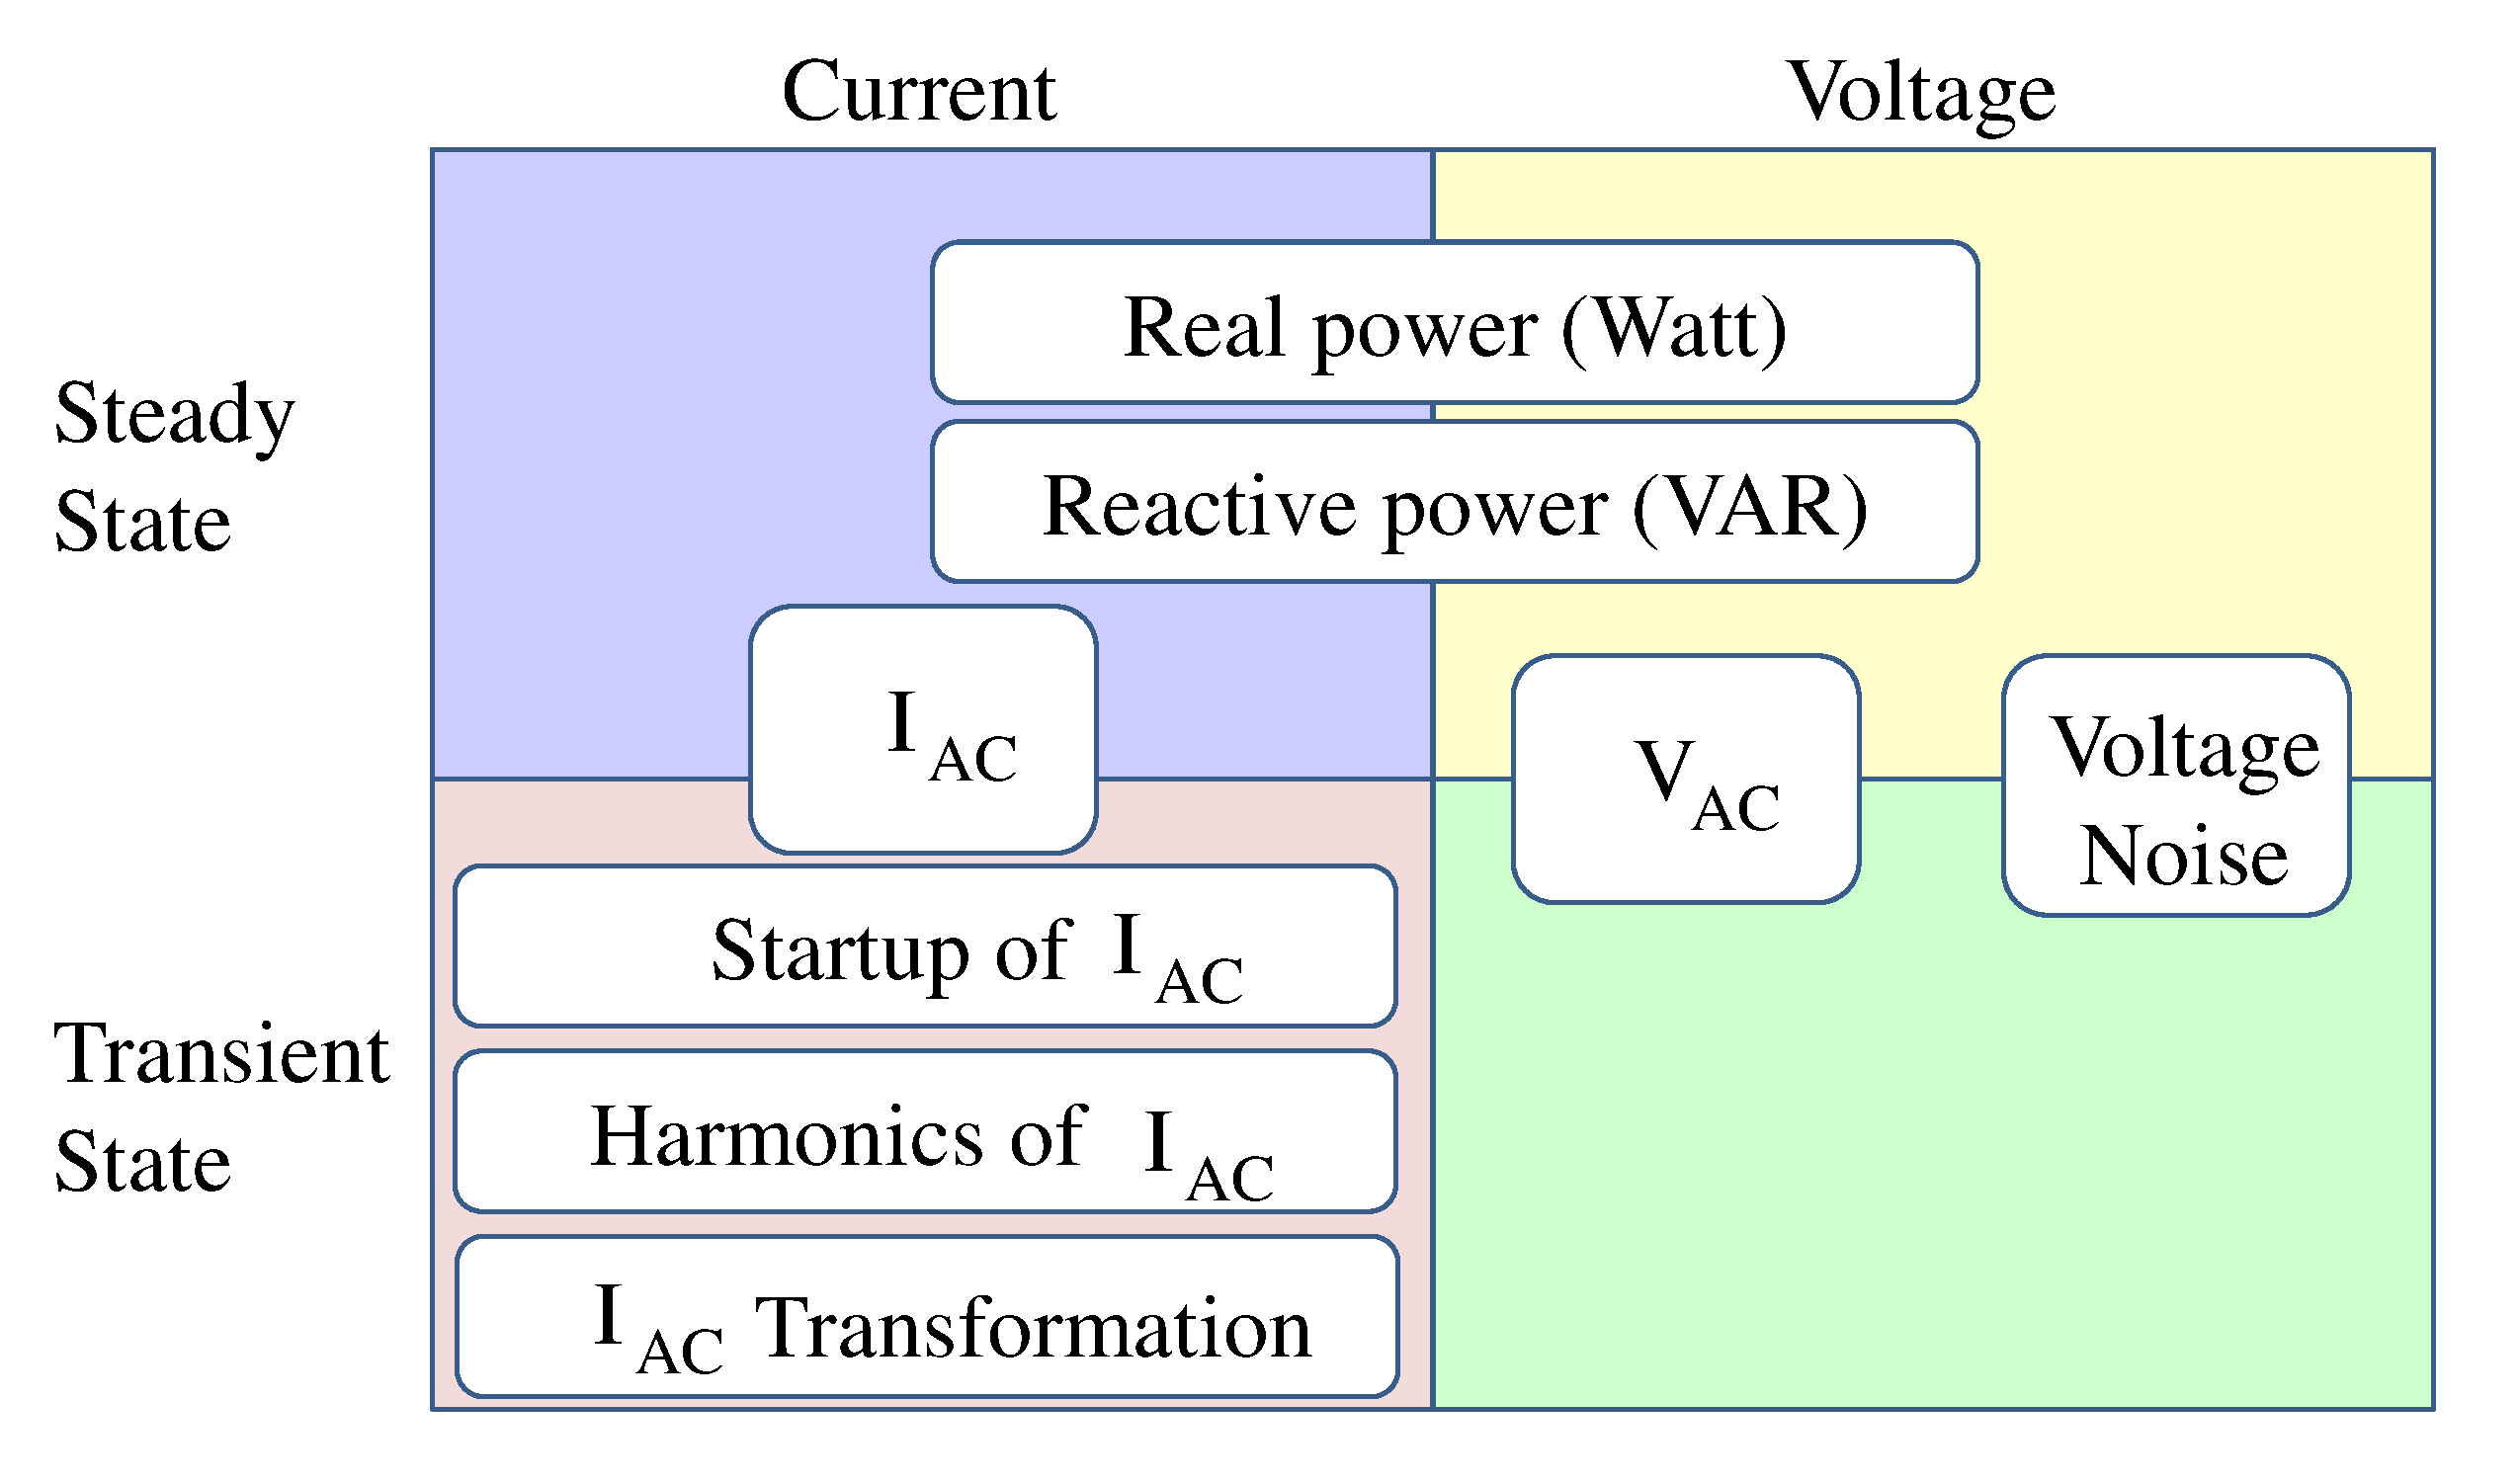
\includegraphics[width=0.45\textwidth]{figs/fig_acpower.pdf} \hspace{1em}&	
	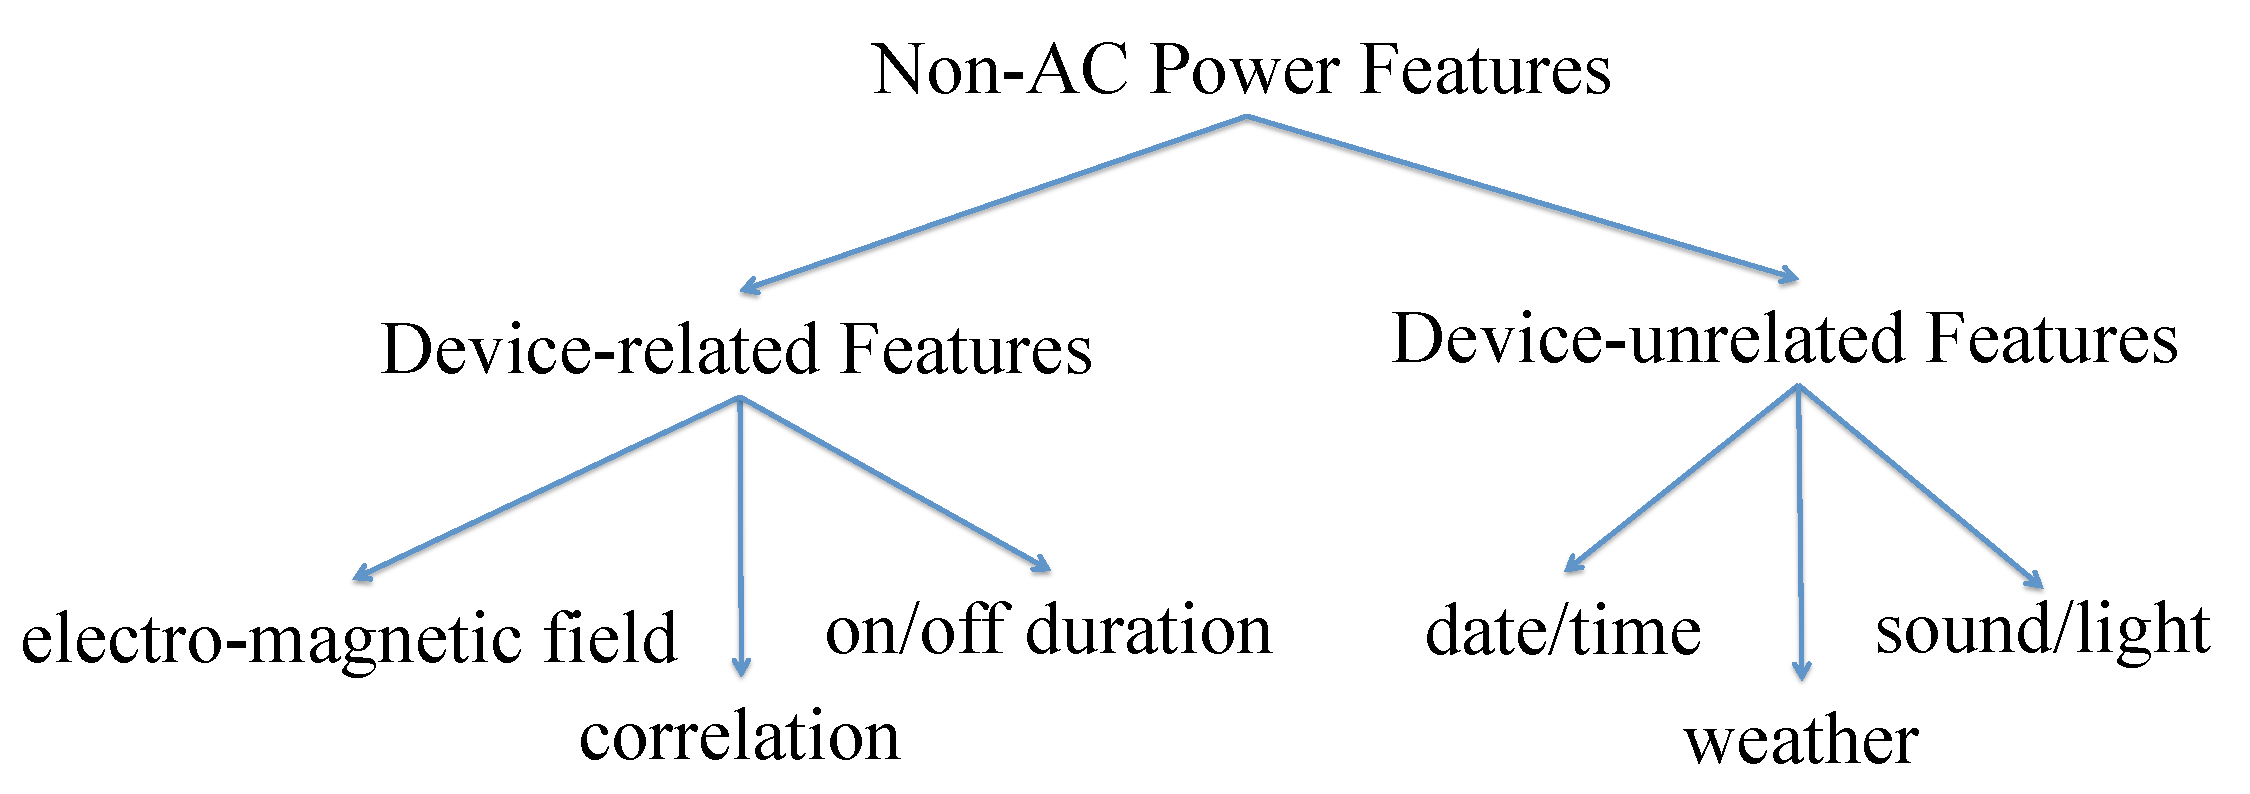
\includegraphics[width=0.55\textwidth]{figs/NonPowerFeatures.pdf} \tabularnewline
    \end{tabular}
    }
	\caption{Category of (a) AC Power Features and (b) Non-AC Power Features. }
	\label{fig_ACPowerFeatures}
\end{figure*}
	

Figure~\ref{fig_ACPowerFeatures} (a) displays a classification of AC power features.
AC power features are related to current or voltage.
These features can also be classified based on the stability of operating states.
(In the below, a
steady state refers to the stable state after a device turns on.)
For example, real power, reactive power, and apparent power
are all steady state features.
Transient states refer to variable states during a very
short period of time when a device turns on or off.
Transient state features are generally derived from
the startup shape of current, voltage,
harmonics or harmonics transformations.
%\begin{figure}[h]
\centering
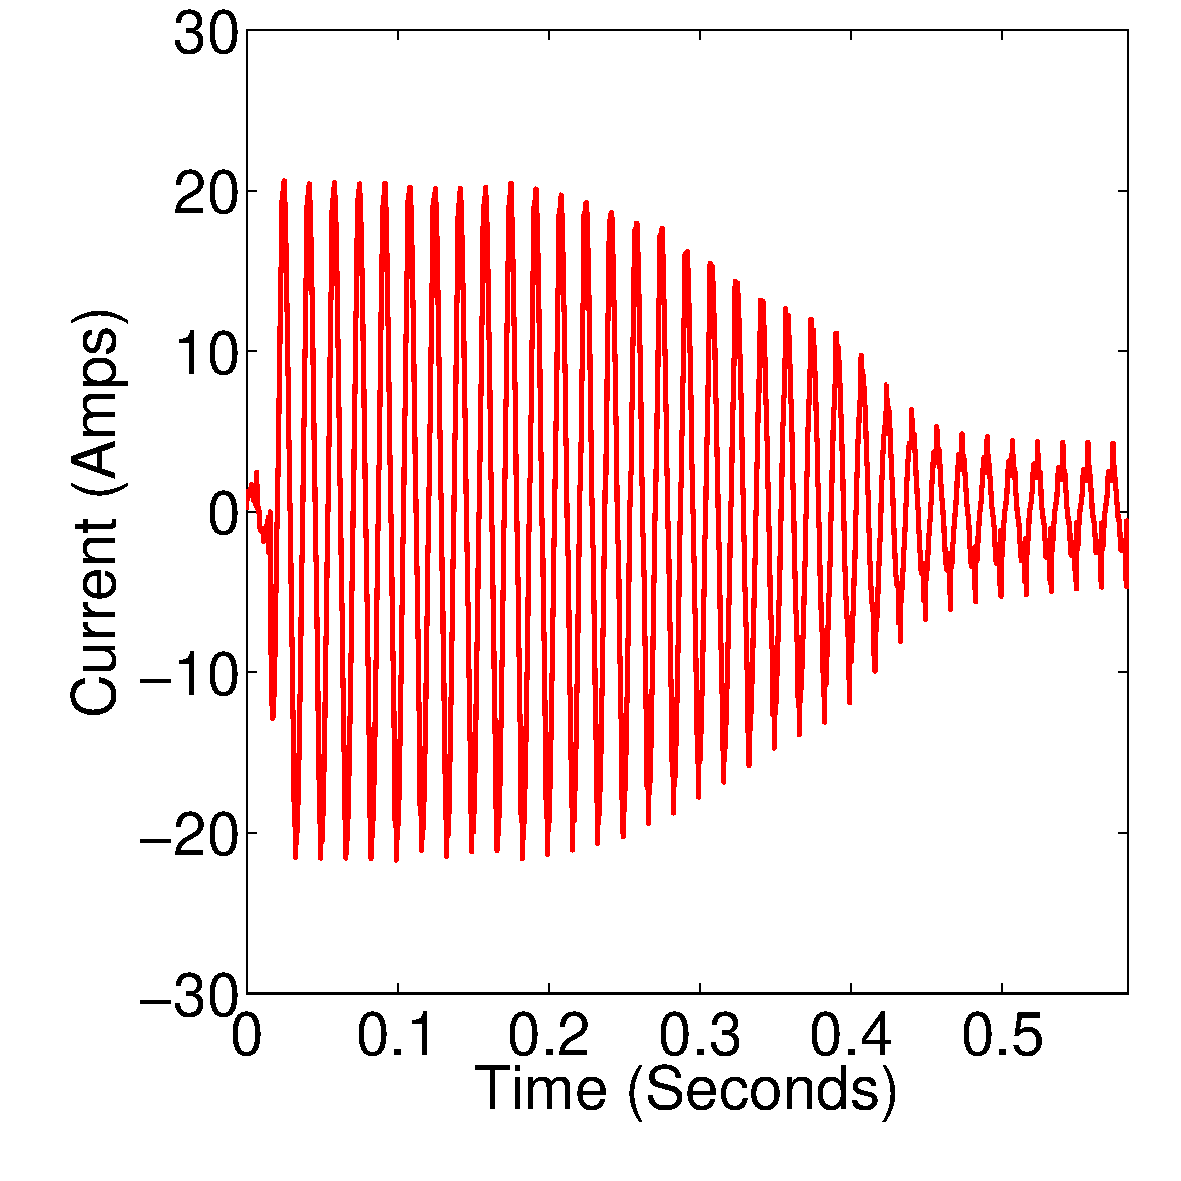
\includegraphics[width=2.5 in]{figs/refrigeratorTransient.pdf}
\caption{Transient and Steady State of a Sinusoidal Current from a Refrigerator.}
\label{fig_transientexample}
\end{figure}

%Any current or voltage is the sum of a transient state 
%and steady state as a function of time. 

Non-AC power features are summarized in %Table. \ref{tab_nonacpower}.
Figure~\ref{fig_ACPowerFeatures} (b). 
%Figure\ref{fig_NonACPowerFeatures}. 
%\begin{figure}[h]
\centering
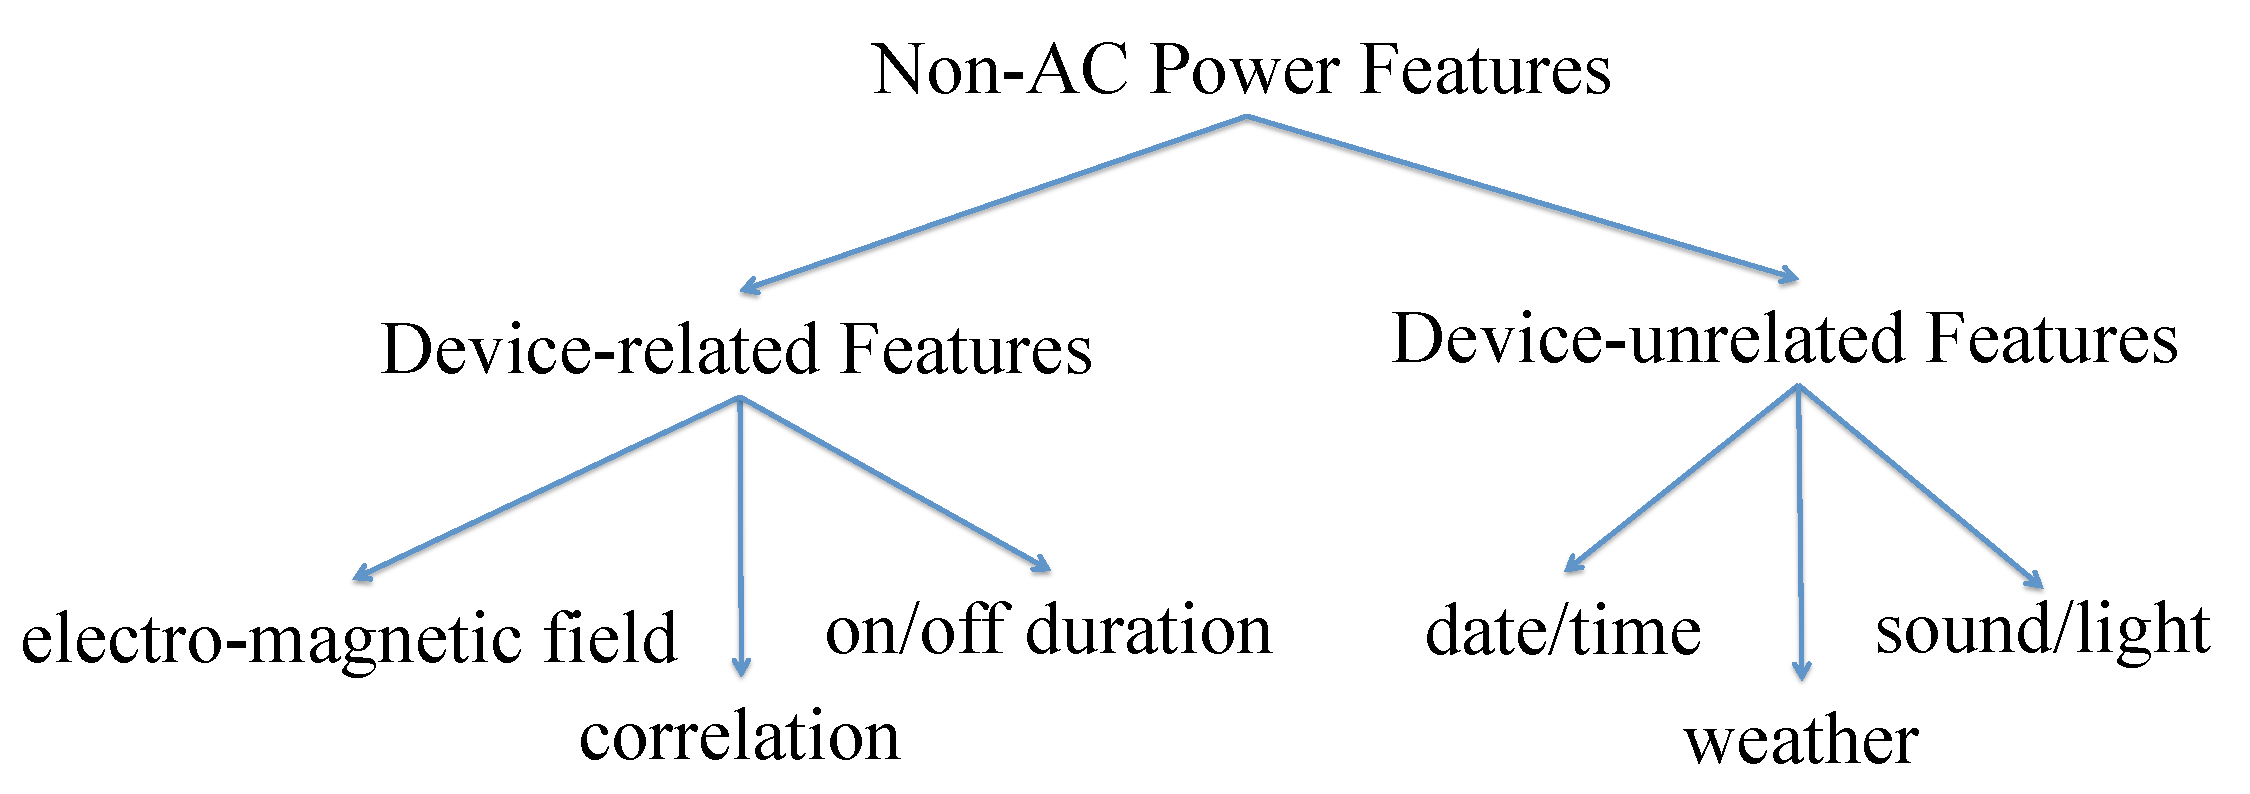
\includegraphics[width=3.5in]{figs/NonPowerFeatures.pdf}
\caption{Category of AC Power Features.}
\label{fig_NonACPowerFeatures}
\end{figure}

These non-AC power features can be classified into two categories:
device-related and device-unrelated. 
%\manishc{call these device-related and device-unrelated features}\huijuanc{ok.Done.}
Device-related category includes electromagnetic field (EMF); 
operational information such as on/off durations, and
 correlation between devices.
%\manishc{where is on/off duration of a device used as a feature?}  
%\huijuanc{in the paper of \cite{kim2011unsupervised}, the on/off duration is used in the semi-FHMM Model.}
The EMF is produced when certain devices are on. 
The device-unrelated category is comprised of 
date or time features, such as month of the year,
day of the month, day of the week and time of the day.  
Also, it includes the ambient temperature, which
plays a crucial role in determining the functioning
of the HVAC system.
%When the weather is hot outside - the cooler is turned on and in
%the cold season the heater is used. 
Further the device-unrelated category include features like sound and 
light produced by an electrical device. 
A sensor can be installed near a device 
to record such features.  

\subsection{AC Power Features}
\subsection{Steady state}
\iffalse
\huijuanc{comment out until huijuan's next comment}
As shown in Figure~\ref{fig_ACPowerFeatures}, 
steady state features include real and reactive power from both 
low frequency and high frequency data, 
current or voltage from high frequency data, 
and voltage noise. \manishc{figure 11 doesn't show anything about high/low frequency} 
\huijuanc{agree. rewritten as follows.}
\fi
As shown in Figure~\ref{fig_ACPowerFeatures}, 
steady states include real power, reactive power, 
current, voltage, 
and voltage noise. 
This data can be either read directly from meters
sampled at low frequency or calculated indirectly from 
high frequency voltage and current data. 
\iffalse
\manishc{in this sentence, are
  you saying the meters that sample at low frequency compute the real/reactive
  power, while the meters that sample at high frequency do not?} 
  \huijuanc{Yes, this is what I mean. Is it correct?}
\fi  
Suppose the basic current/voltage frequency of
AC power, $\omega$, is 60 Hz
and the sampling frequency of recorded data is $f$,
i.e., there are in total $f/60$ number of sample points in
each cycle.
The real power value is the average product
of current and voltage in a cycle as in Equation (\ref{eq_realpowerhighfreq}). 
\begin{equation}
P_{av}= \frac{\sum_{t}^{t+f/60} v(t) \cdot i(t)}{f/60}
\label{eq_realpowerhighfreq}
\end{equation}
%When introducing the angle phase difference between current and voltage, 
%we can also calculate the instantaneous reactive power according to 
%Equation (\ref{eq_powerTriangle}) in section~\ref{sec_pvCalculation}.
%\manishc{how do you compute the reactive power from that equation? It has
 % apparent power as well, where do you get that from?}

Real power is the most basic feature and used 
by almost all prior work in energy disaggregation \cite{hart1992,powers1991using,farinaccio1999using,marceau2000nonintrusive,baranski2004genetic,baranski2004detecting}.
Reactive power is also widely used as a feature, e.g., in \cite{hart1992,laughman2003power,drenker1999nonintrusive}.
Figure~\ref{fig_realReactive_hart1992} shows real power and 
reactive power features of different devices. 
For some devices real and reactive power are sufficient to distinguish
between them. 
A refrigerator and water pump have similar reactive power but
different real power; thus using the real power feature, we can separate them. 
A refrigerator and garage door opener have similar real power but different reactive power;
thus the reactive power is the distinguishing feature in this case.
Steady state features are also derived from the variations of real or reactive power.
For instance, in~\cite{milioudis2013event}, 
the slopes of both active and reactive power 
are extracted as vectors. % as shown in Figure\ref{fig_ACPowerFeatures}. 


\subsection{Transient state}
High frequency data, 
from which the current waveform or voltage waveform can be recovered, 
%\manishc{what does
%  ``reconstructed'' mean here; you are already measuring current/voltage at
%  high frequency. You may want to reword/explain.}\huijuanc{I mean the waveform of the current 
%  or voltage can be reconstructed. }
offers rich features that can be applied to energy disaggregation. 
These features include the startup of current, 
harmonics of current, 
harmonics of voltage, 
voltage noise and its transformations. 

\textit{Startup duration and transient power:}
Startup duration and transient power are recorded when a device is turned on. 
Usually a non-linear device, like a microwave, has such a distinguishing feature.
%\manishc{not clear what this means, please re-word}.    
When this kind of device turns on,
the power usage usually changes to a temporary high value for few 
or milliseconds, %\manishc{this is too high! do you mean millisec?}\huijuanc{yes. already updated}, 
then jumps into a steady state for a longer time.
This temporary startup duration and shape feature varies from one device to another. 
Comparing the transient power changes with the steady state, 
the trail of power changes against time looks like a spike or a curve with changing slope. 
Figure~\ref{fig_realTransient} shows examples of current, average real power and instantaneous
real power in the first 0.5 seconds of a refrigerator turning on in the 
BLUED dataset~\cite{anderson2012blued}. 
\iffalse
 \manishc{you said 0.5 sec in the previous
  sec; make it consistent, and this sentence seems like a repetition} \huijuanc{updated, and remove the repeated sentence}. 
\fi  
In Figure~\ref{fig_realTransient} (a), there are three areas in this waveform.
When $0<t<0.02s$, the current is in
a steady state.
When $0.02s \leq t \leq 0.45s$,
the current is in a transient state,
during which the amplitude of the current changes
rapidly. 
%\manishc{the amplitude of the current is changing, but the frequency
 % doesn;t seem to change much.}\huijuanc{agree. updated.}
When $ t \geq 0.45s$, the current comes again to a
steady state.
Figure~\ref{fig_realTransient} (b) shows the shape of corresponding average power. 
\iffalse
\manishc{i assume this is average power? please call it average power,
  since you are talking about instantaneous power here as well} \huijuanc{done.}
It reaches around 400 watts for a very short period of time 
\manishc{i don;t
  see it being 400 W in fig 12 (b)}\huijuanc{deleted}
\fi 
It jumps to 1600 watts in a very short period of time, then gradually decreases to 200 watts (calculated using
Equation (\ref{eq_realpowerhighfreq})).
Figure~\ref{fig_realTransient} (c) depicts the instantaneous real power. 
There are 200 points in each cycle. As can be seen, the
instantaneous power changes very frequently.
\begin{figure*}[ht]
	\centering{
    \begin{tabular}{ccc}	
    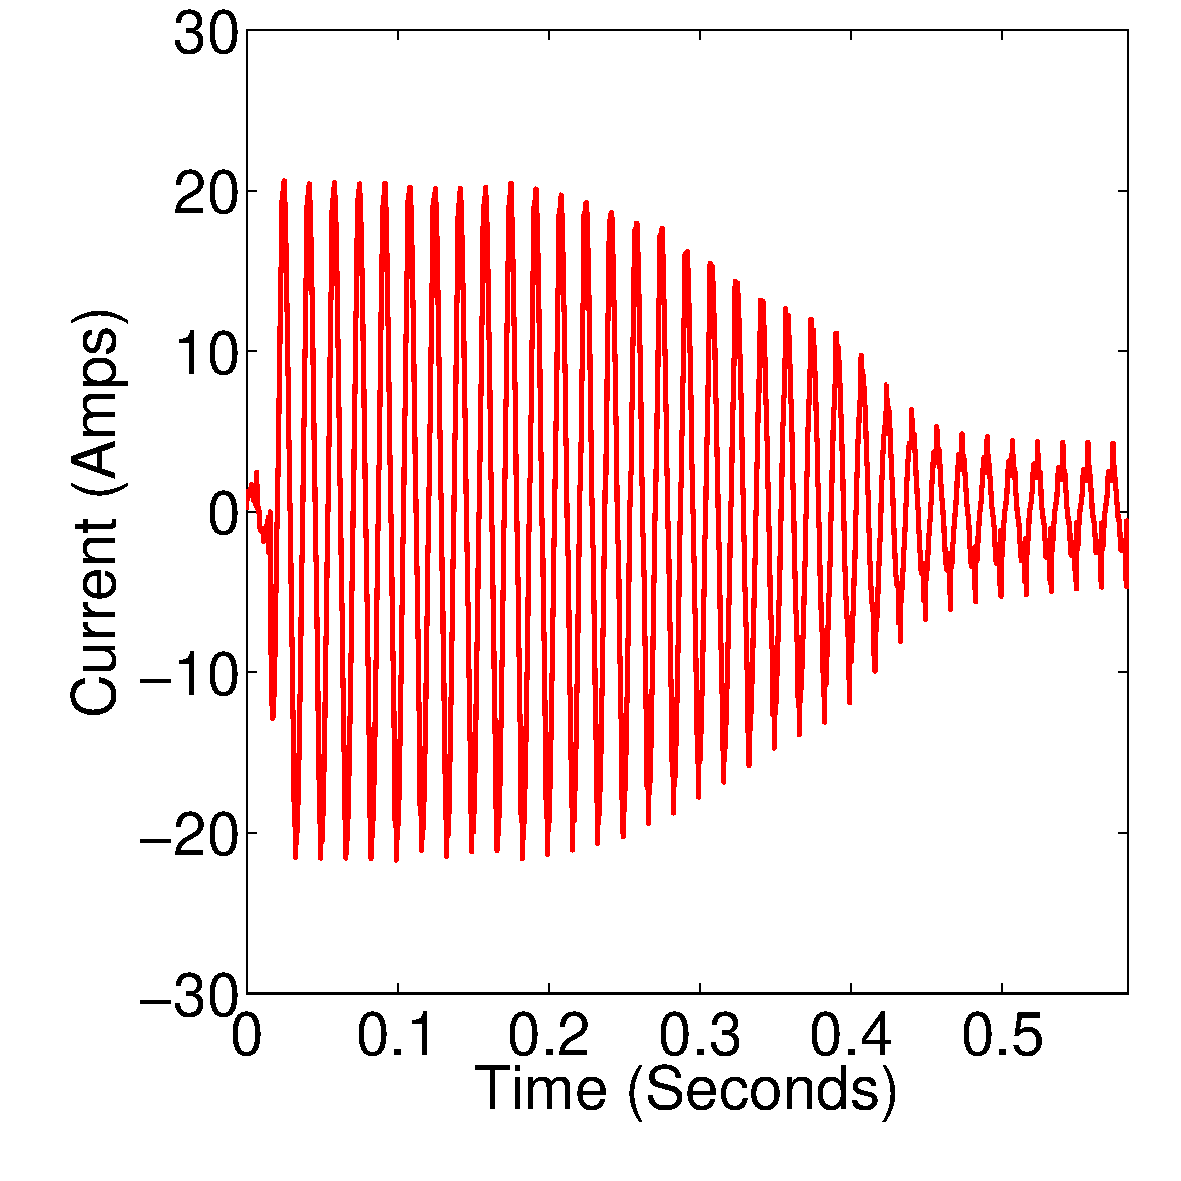
\includegraphics[width=0.29\textwidth]{figs/refrigeratorTransient.pdf}                 \hspace{1em}&
    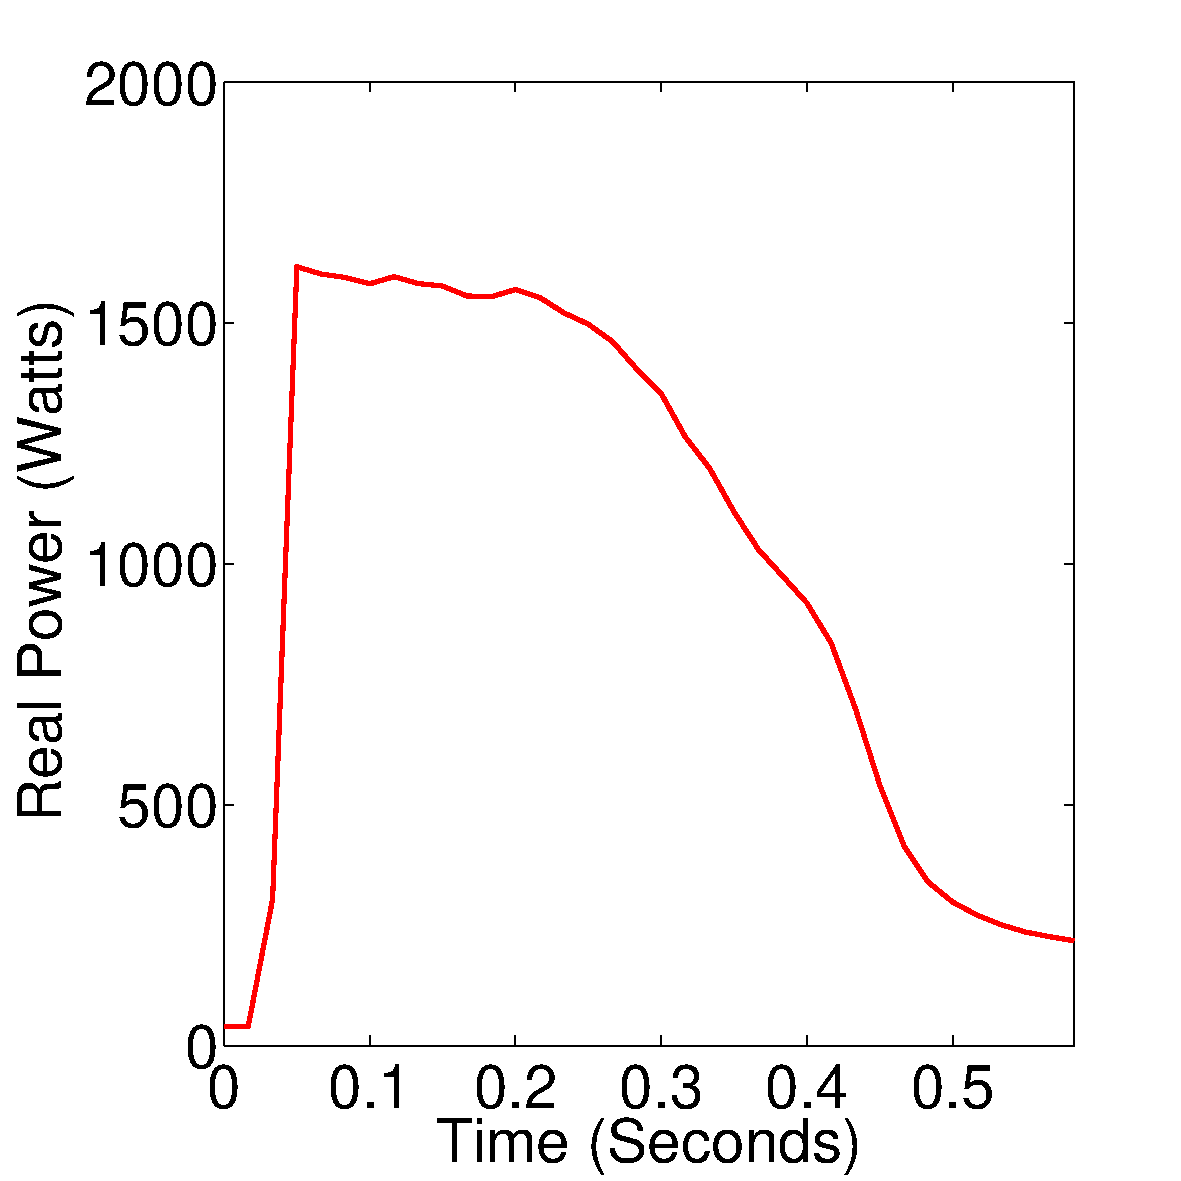
\includegraphics[width=0.3\textwidth]{figs/refrigeratorTransientRealPower.pdf} \hspace{1em}&
    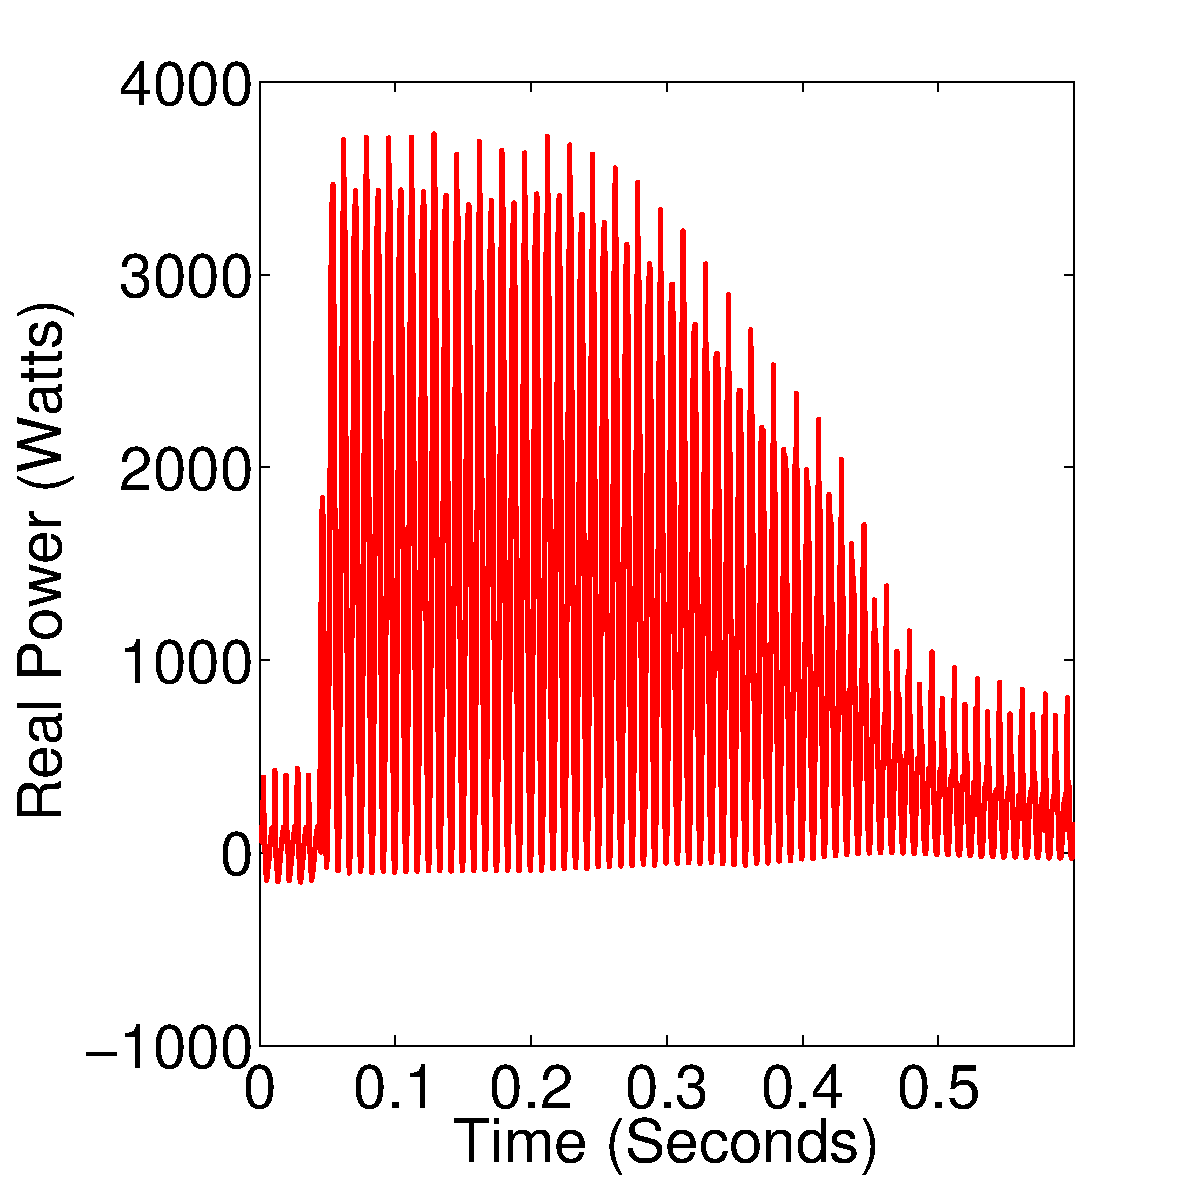
\includegraphics[width=0.3\textwidth]{figs/refrigeratorTransientInstantPower.pdf} \tabularnewline
    (a) & (b) & (c)\tabularnewline
    \end{tabular}
    }
	\caption{(a) Transient and Steady State of a Sinusoidal Current from a Refrigerator. Transient Shapes for a Refrigerator (b) Real Power and (c) Instantaneous Real Power.}
	\label{fig_realTransient}
\end{figure*}

%transient.tex
%\begin{figure}[h]
%\centering
%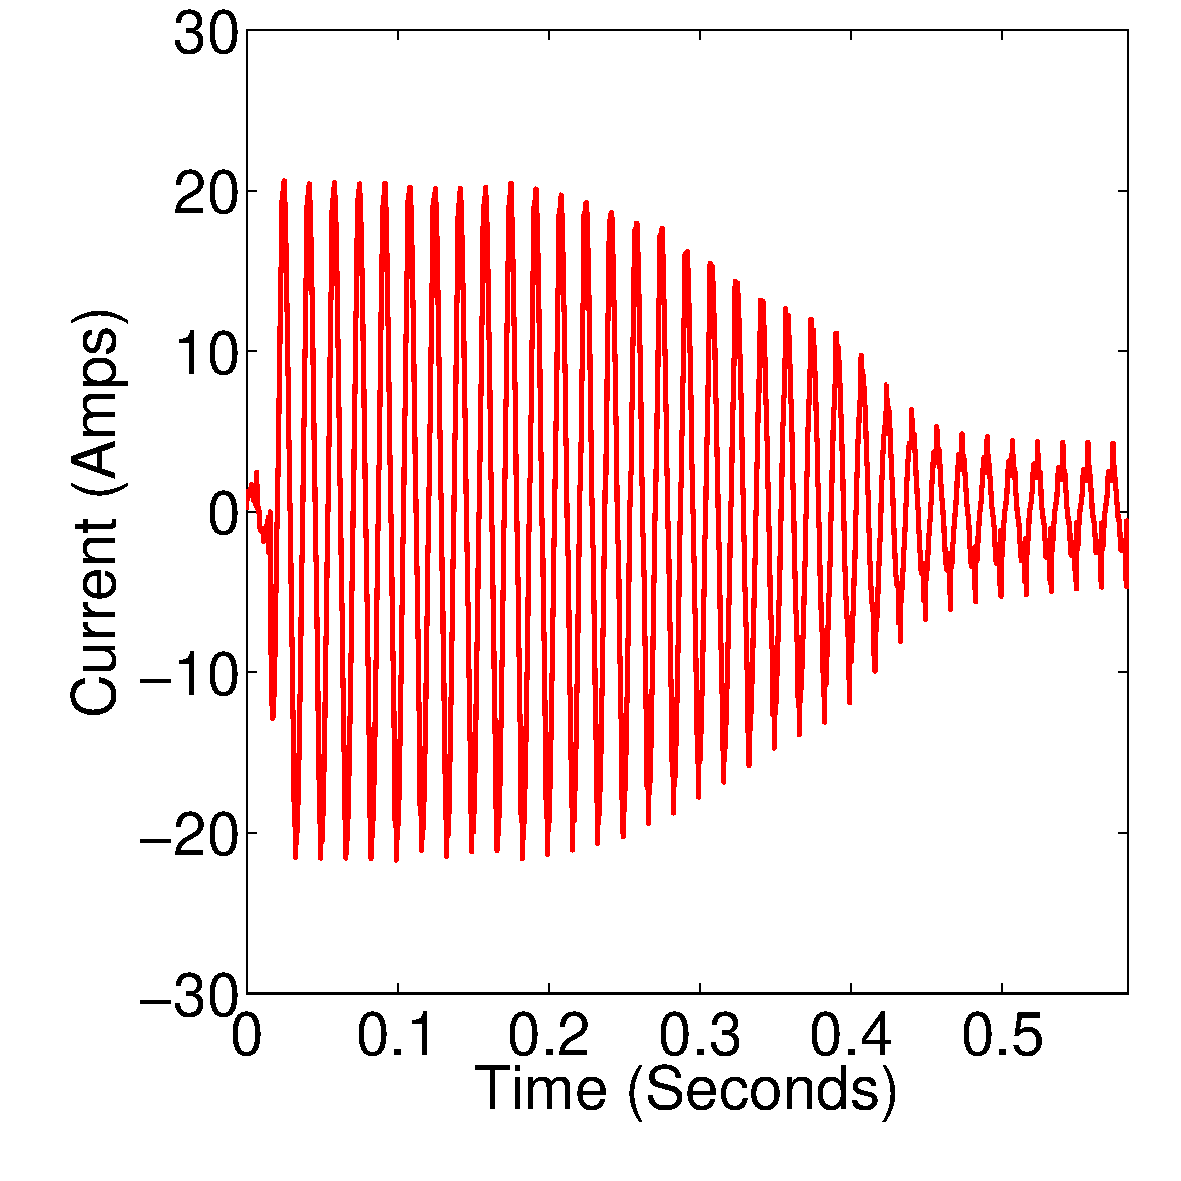
\includegraphics[width=2.5 in]{figs/refrigeratorTransient.pdf}
%\caption{Transient and Steady State of a Sinusoidal Current from a Refrigerator.}
%\label{fig_transientexample}
%\end{figure}

The transient energy %\manishc{real power?} \huijuanc{change power as energy} 
is calculated as 
$E_{transient} = \int_{t_s}^{t_s+\delta t} v(t)i(t)dt $, 
where $t_s$ is the start time and $\delta t$ is the startup duration. 
The corresponding real power is calculated as 
$P(t) = \frac{dE_{transient(t)}}{dt} = v(t)\cdot i(t)$.
\iffalse
\manishc{this is confusing, is ``transient power'' ``transient real power''?
  what is the unit of transient power? is it Watts? from your equation of
  $P_{transient}$ it appears to be Watt Second? can you verify these
  equations, and explain how transient power is different from real power. I
  initially thought that transient power is just the power during the
  transient period; is that correct?}\huijuanc{already verified the equation and changed it.}
\fi  
%\begin{eqnarray*}
%W_{transient} = \int_{t_s}^{t_s+\Delta t} v\cdot i \cdot dt \\
%\end{eqnarray*}

This startup duration and shape of current or power feature can be used 
standalone or in integration with other features.
~\cite{sultanem1991using} gives a typical example of the latter case. 
The startup duration and the shape of current or power feature 
is combined with real power and reactive power
to distinguish each device among refrigerator, washing machine, and fluorescent light.
Note that 
this transient startup may be called transient spectral envelope~\cite{shaw2000PhdThesis}, 
or transient power. 
%It has been applied in previous work
%as features to identify electrical device.(?give an example)

\textit{Current or voltage waveform:}
The current waveform $I_{ac}$, which can be simply read from
high frequency recorded data,
is a typical feature used to discriminate devices.
The waveforms generated by non-linear devices  are 
very different due to the waveform distortion 
introduced by each device. 
Figure~\ref{fig_waveformTraj} (a-b)
illustrates the current waveform 
of two devices---refrigerator and compressor---from the
BLUED dataset. 
From them, we can see that both the magnitudes  and the distortions 
of the current waveforms differ from each other. 
The maximum current magnitude of a refrigerator is 20 Amps while that of 
the compressor is around 16 Amps. 
%\begin{figure*}[ht]
	\centering{
    \begin{tabular}{cc}	
	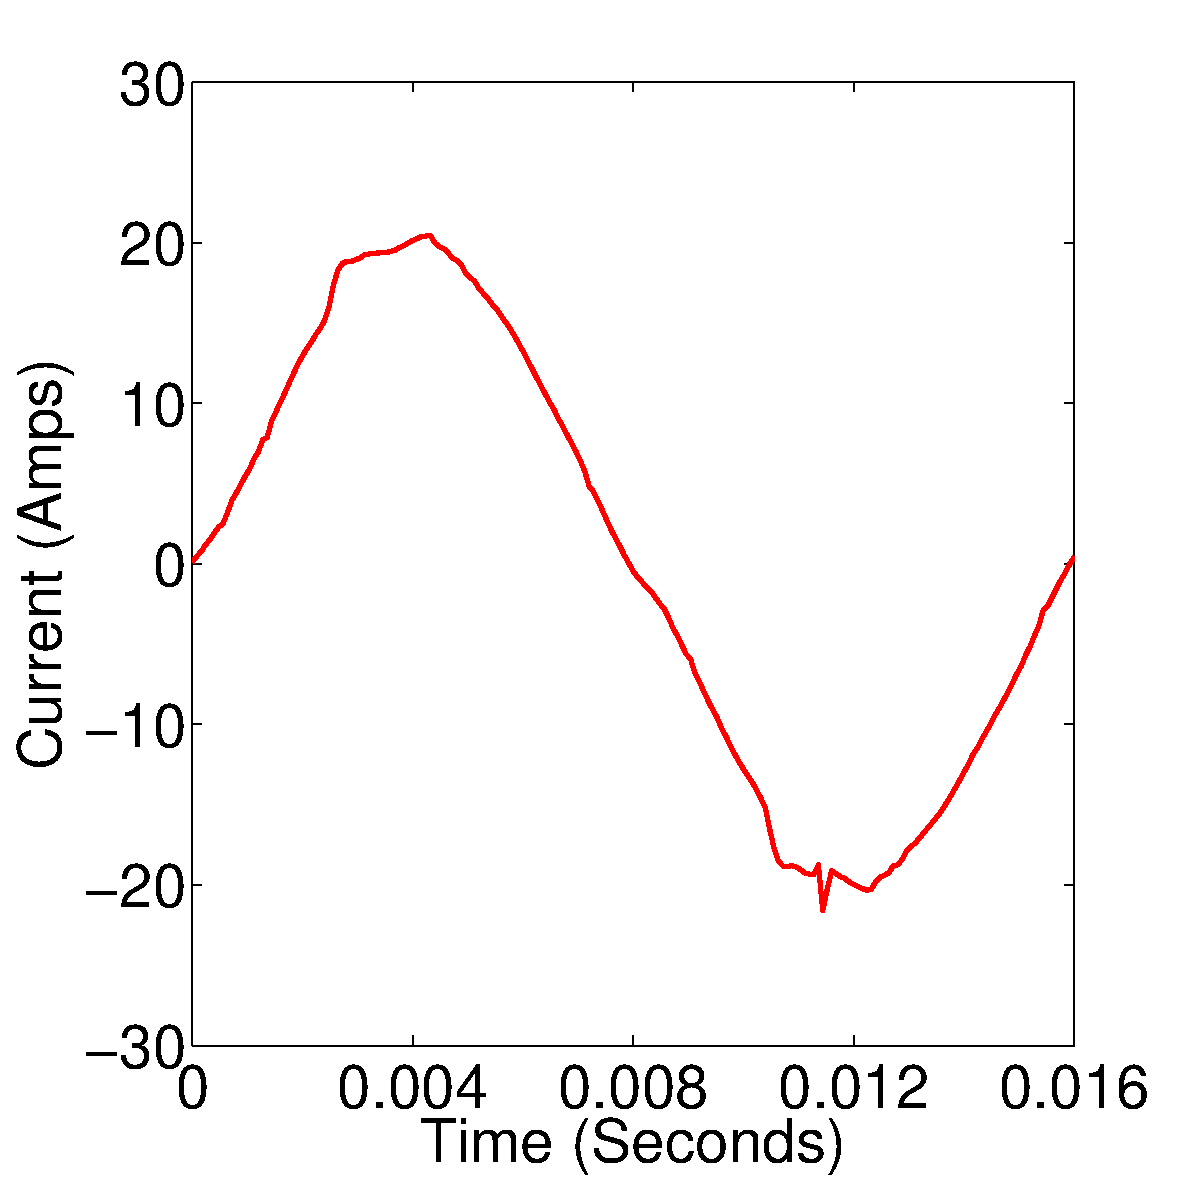
\includegraphics[width=0.5\textwidth]{figs/refrigeratorTransientSingle.pdf} \hspace{1em}&
    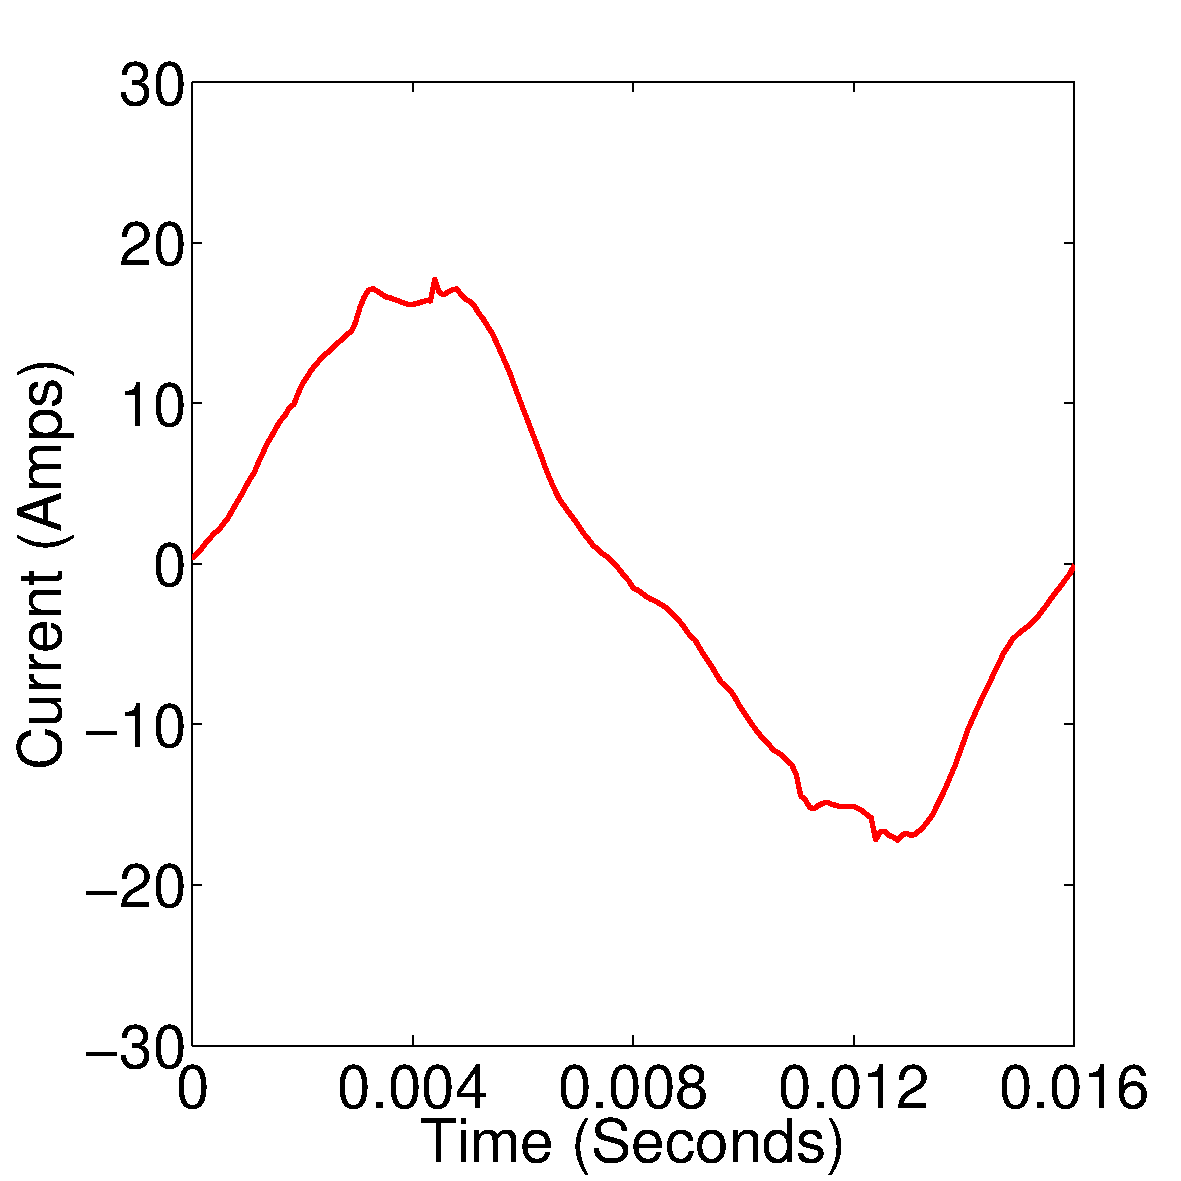
\includegraphics[width=0.5\textwidth]{figs/airCompressorTransientSingle.pdf} \tabularnewline
    (a) & (b) \tabularnewline
    \end{tabular}
    }
	\caption{Current waveform of (a) a refrigerator and (b) an air compressor.}
	\label{fig_currentwaveform}
\end{figure*}
 

Current or voltage waveform features have been applied in previous work.
The unprocessed current waveform 
%just like waveform in Figure~\ref{fig_currentwaveform}, 
is regarded as a feature in~\cite{suzuki2008nonintrusive}.
This paper shows that 
the raw current waveforms of a microwave oven and a toaster oven 
are different in a cycle. 
Therefore, these raw current waveforms can be used to separate 
these two devices. 
However, raw current waveforms are prone to changes with noise.
\cite{duan2004neural} analyze the current waveforms of eight devices and classify
them as A/C, refrigerator, compressor, 
fan (VSD), elevator (converter), elevator (M/G set), fluorescent lights 
and computers. 
Similarly, standalone voltage waveform has been used as a feature in previous work. 
%The distortion is mainly generated by non-linear devices.
By analyzing voltage shapes,
we can determine which device is on.
%The difference of voltage waveform is that the maximum value of 
%voltage is approximately 116V in the U.S.
%\cite{cox2006transient} uses the distortion of voltage waveform to
%separate transient shapes as described in~\cite{srinivasan2006neural}.
While a combination of current and voltage waveforms has been proposed as
features, \cite{hassan2014empirical} show that the disaggregation results 
are better
when adopting either the current waveform or the voltage waveform-based
features exclusively.

In order to overcome the shortcomings of raw current or voltage waveforms, 
several variations or transformations of these waveforms have been proposed. 
The first is the voltage-current (V\-I) or current-voltage (I\-V) trajectory. 
This idea is useful because for
dynamic devices such as an air conditioner,
the current waveform may vary from cycle to cycle.
Figure~\ref{fig_waveformTraj} (e-f) illustrates the current trajectory difference between 
two devices, %\manishc{what is a sequential device?}\huijuanc{not sure. delete sequential}, 
viz a refrigerator and an air compressor in the BLUED dataset. 
From Figure~\ref{fig_waveformTraj} (c) and (d), 
we can see that there is only a slight difference between the current and voltage waveforms.
\iffalse
\manishc{not
  clear, do you mean in subfigures (c) and (d), there is a difference in the
  current and voltage waveforms?} \huijuanc{Yes. I mean little difference not much.}
\fi  
But when comparing the current against the voltage as shown in
Figure~\ref{fig_waveformTraj} (e) and (f), 
the V-I trajectories are quite different. 
 %Circuit4 and dining room light. 
%From it, we can see thtat after the dinning room light is turned on, 
%the current changes some in the first half cycle. 
\begin{figure*}[h]
	\centering{
    \begin{tabular}{ccc}
    	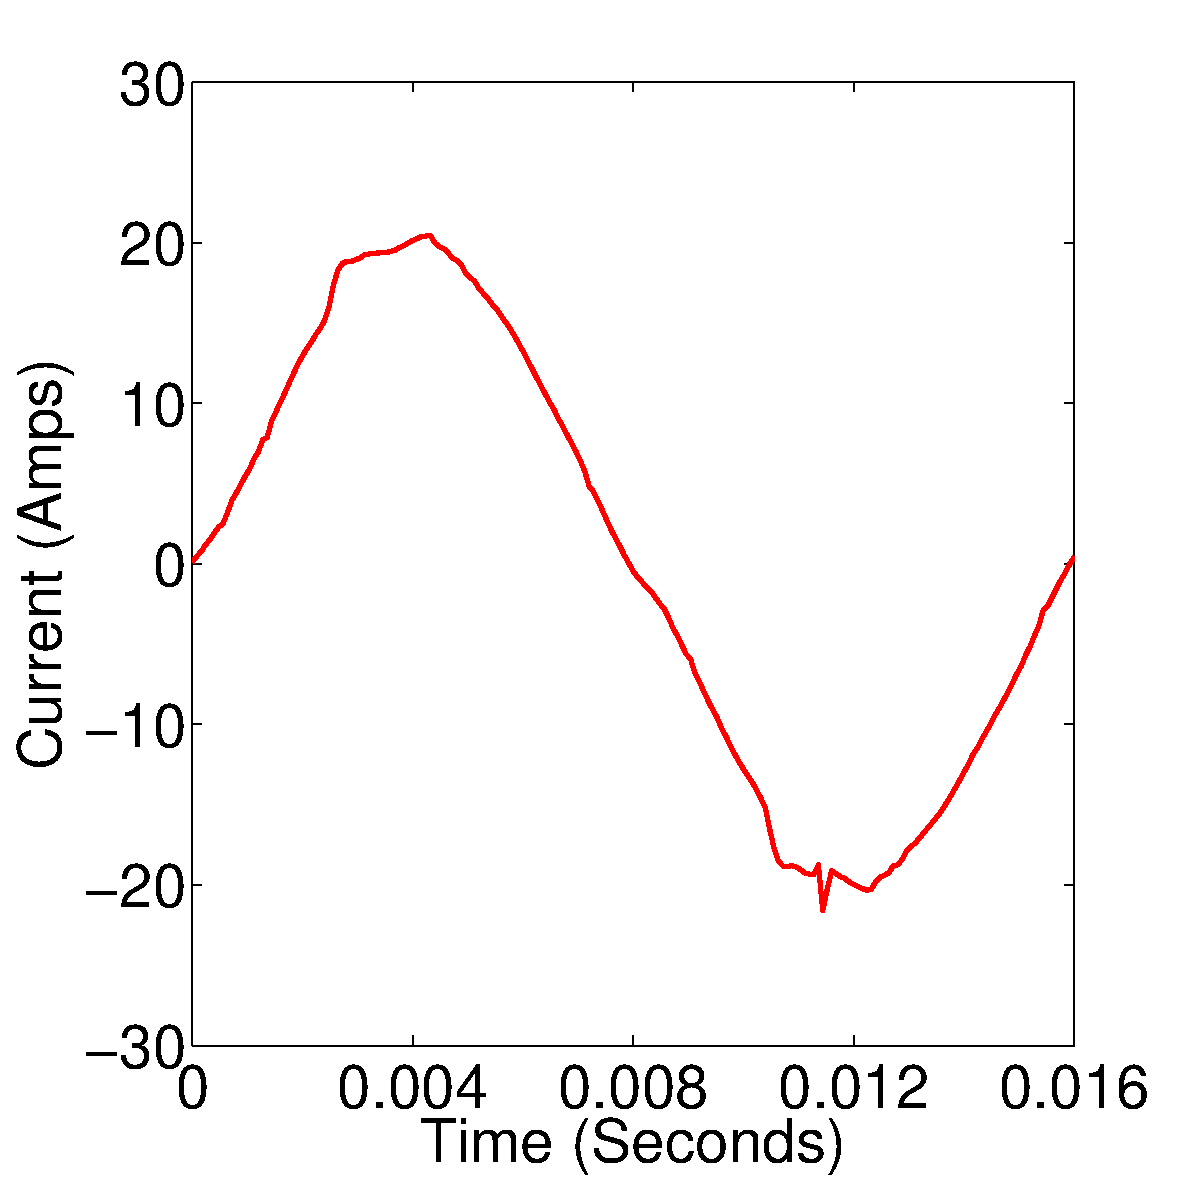
\includegraphics[width=0.3\textwidth]{figs/refrigeratorTransientSingle.pdf} \hspace{1em}&	
	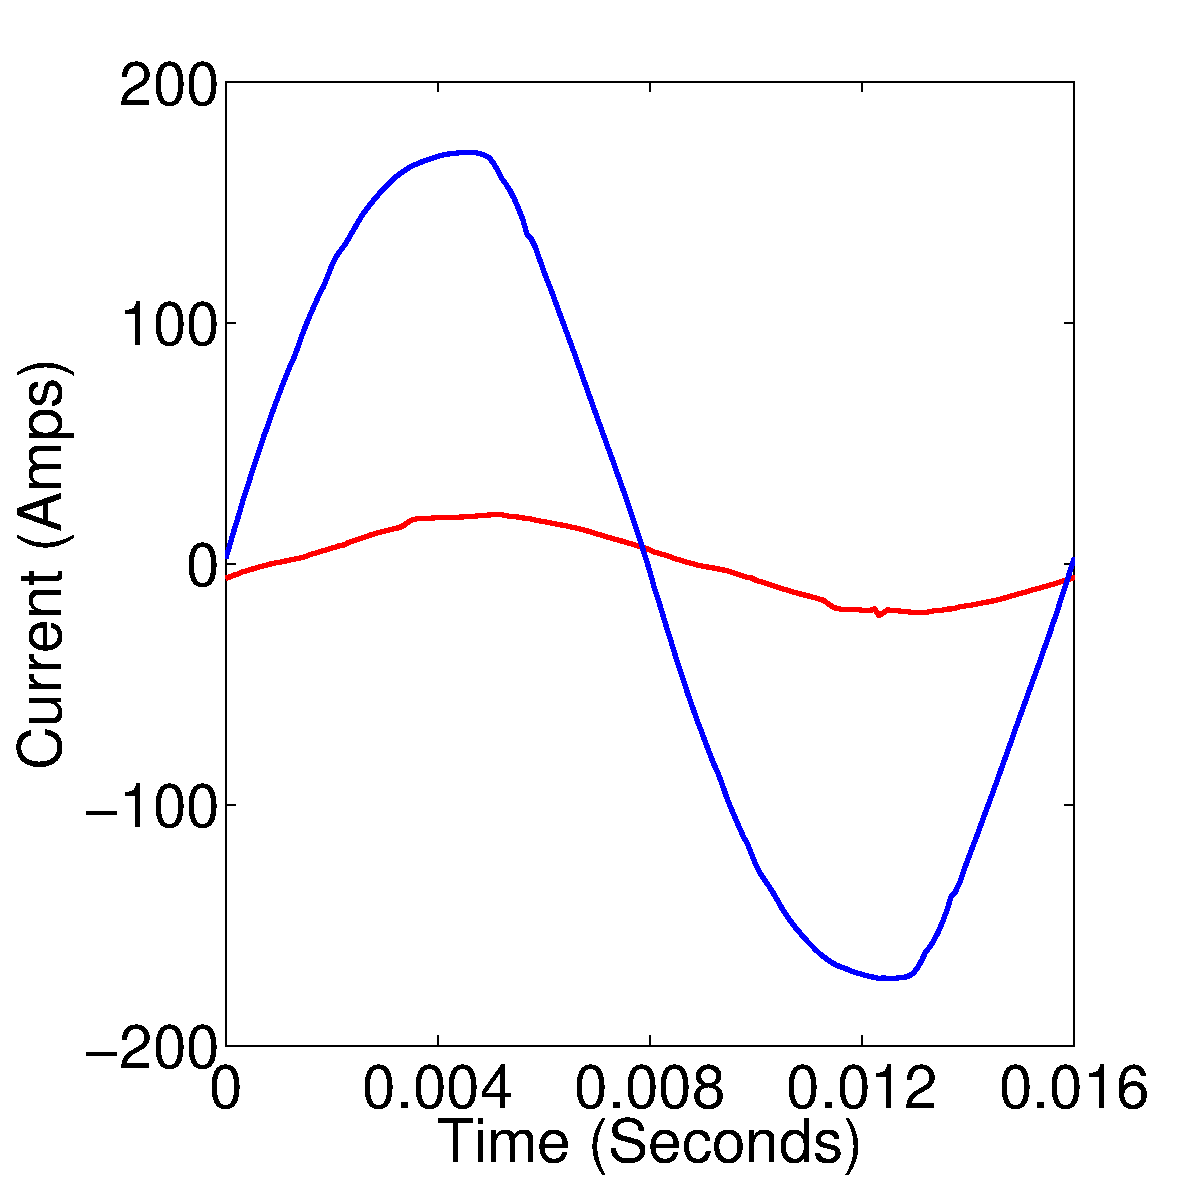
\includegraphics[width=0.3\textwidth]{figs/refrigeratorTransientCurrentVoltageSingle.pdf} \hspace{1em}&
	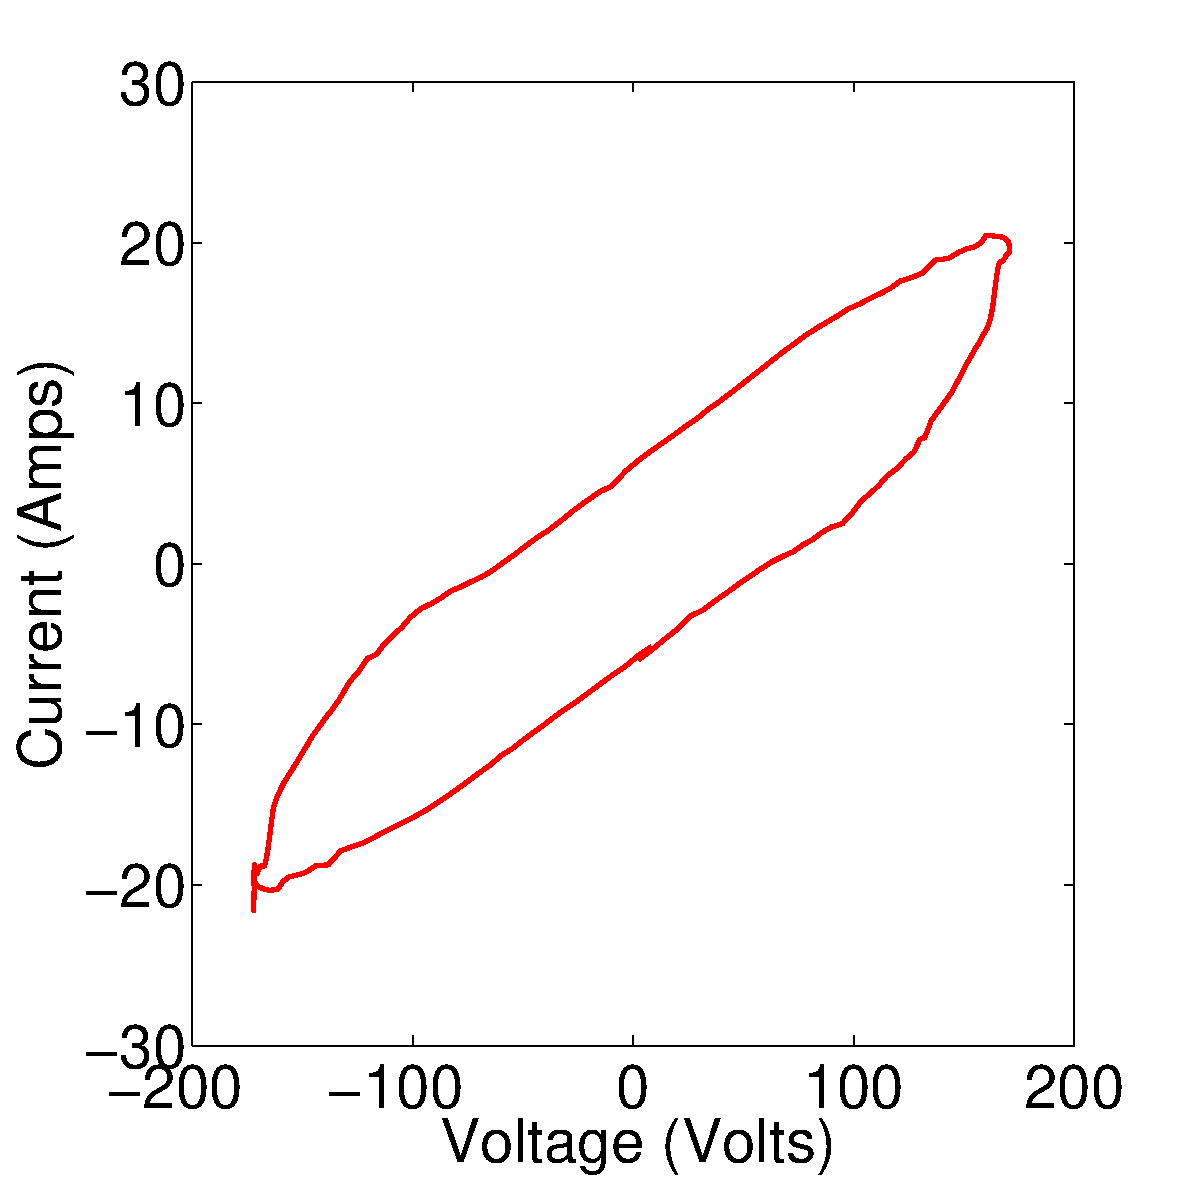
\includegraphics[width=0.3\textwidth]{figs/refrigeratorCurrentAgainstVoltageSingle.pdf} \tabularnewline

    (a) refrigerator & (c) refrigerator & (e) refrigerator \tabularnewline
        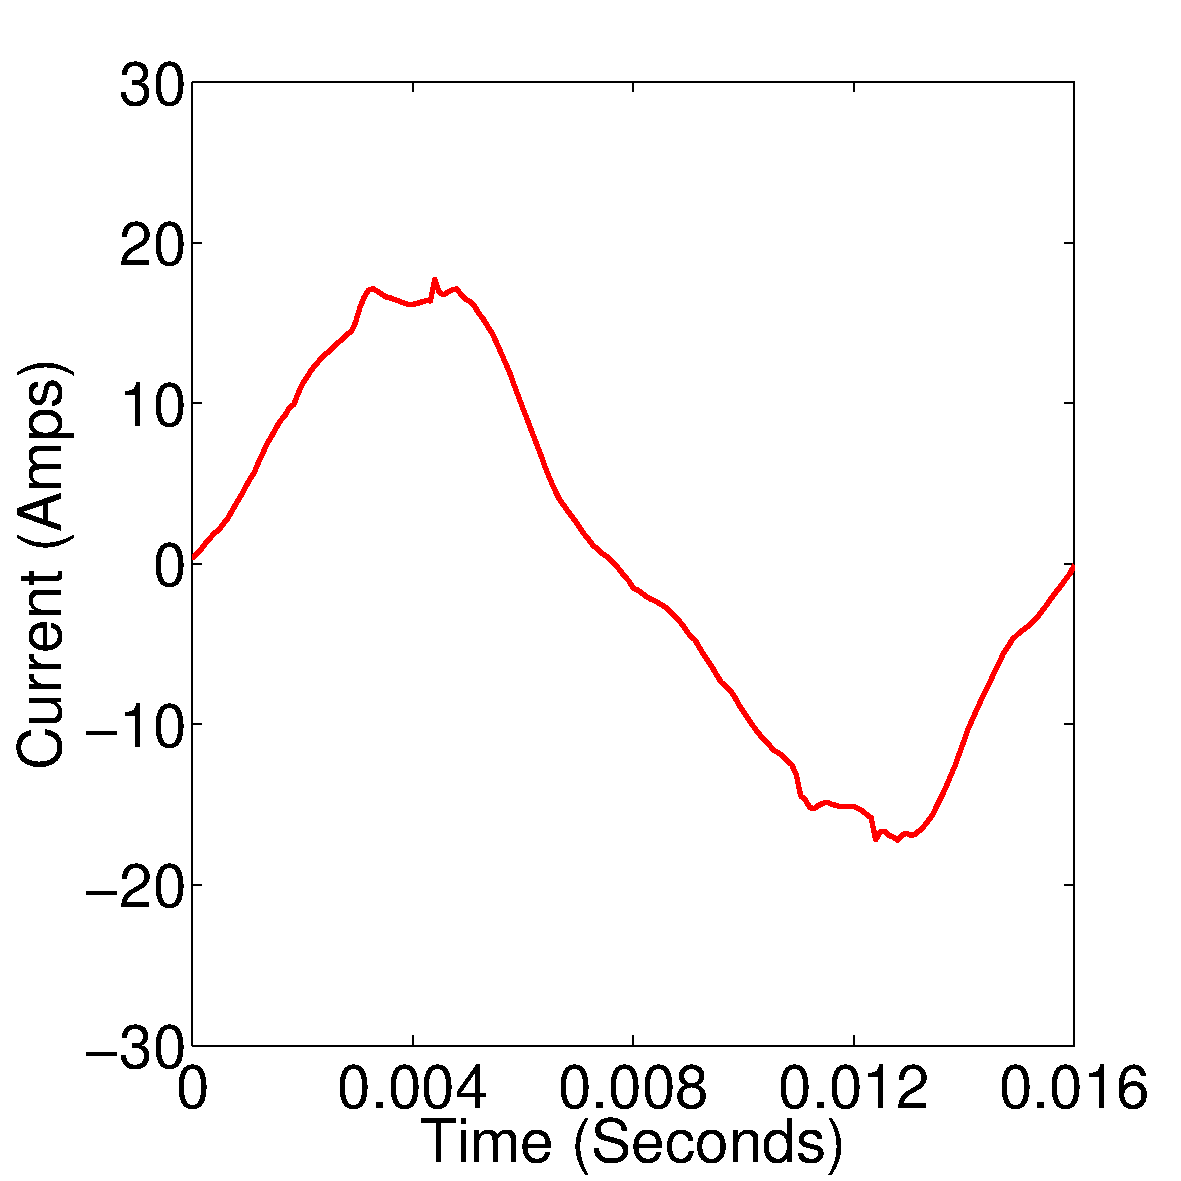
\includegraphics[width=0.3\textwidth]{figs/airCompressorTransientSingle.pdf} \hspace{1em}&	
        	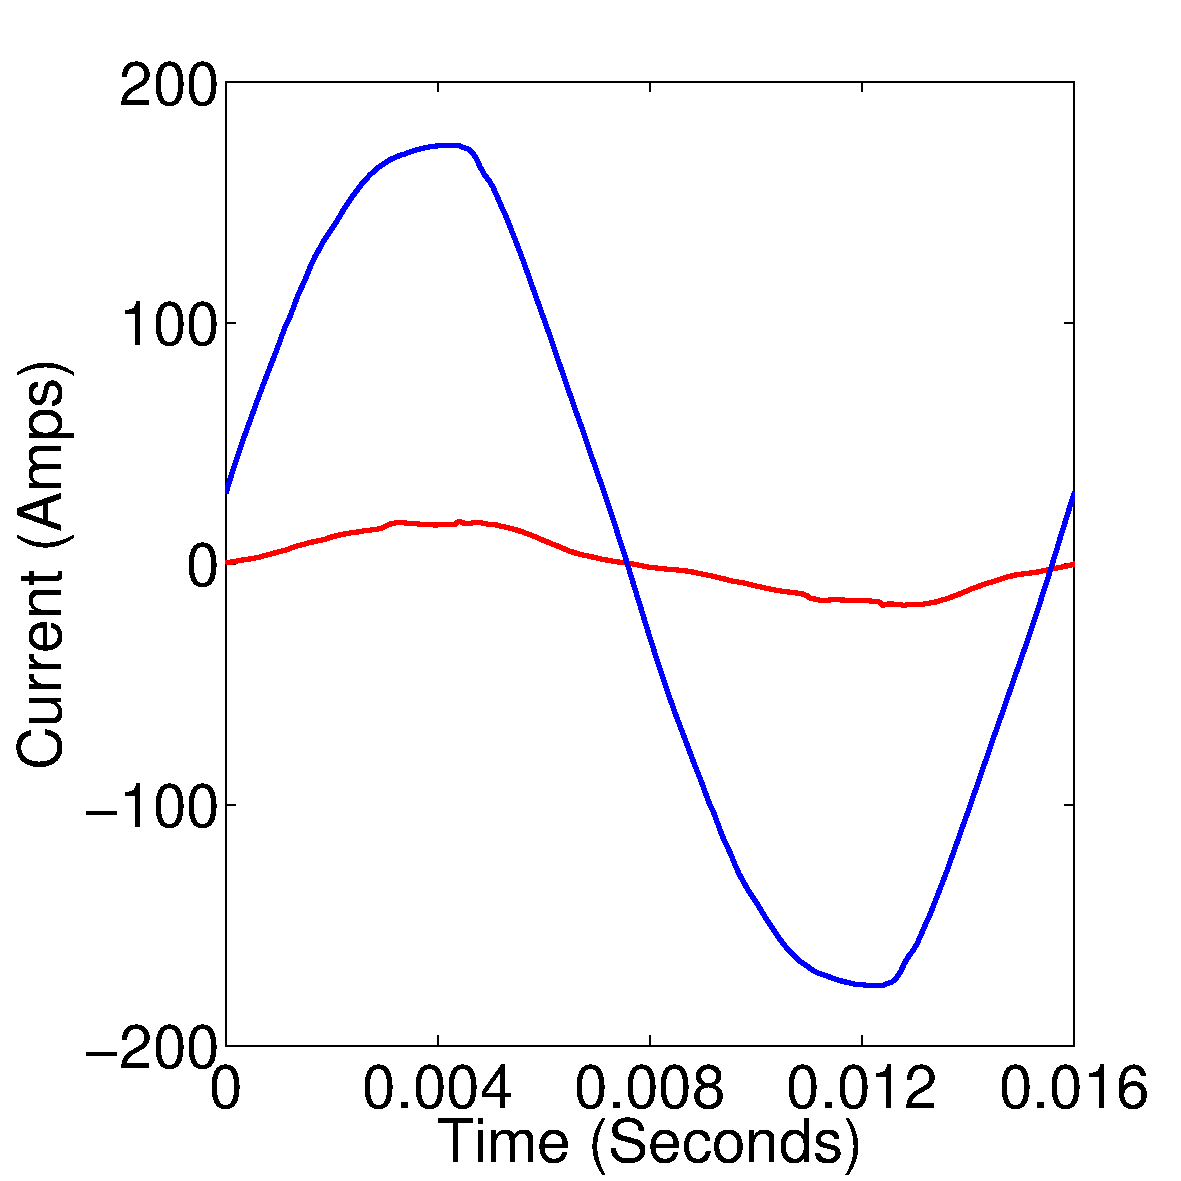
\includegraphics[width=0.3\textwidth]{figs/airCompressorTransientCurrentVoltageSingle.pdf}\hspace{1em}&	
	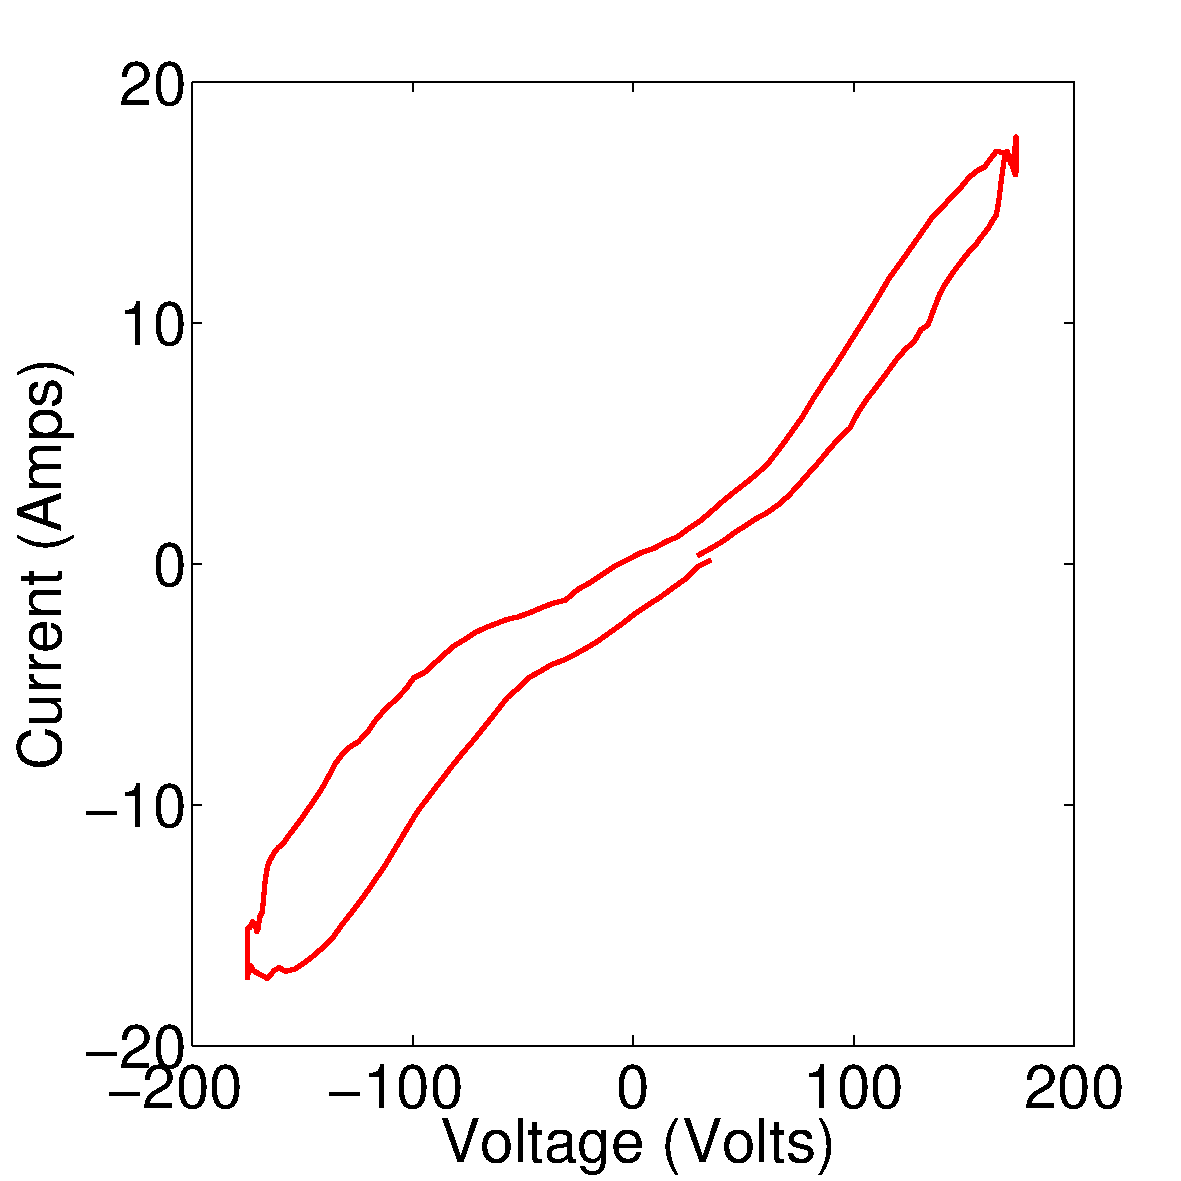
\includegraphics[width=0.3\textwidth]{figs/airCompressorCurrentAgainstVoltageSingle.pdf}\tabularnewline
    (b) air compressor & (d) air compressor & (f) air compressor \tabularnewline
    \end{tabular}
    }
	\caption{Current waveform of (a) a refrigerator and (b) an air compressor. The current and voltage of (c) a refrigerator and (c) an air compressor. The V-I trajectories of (e) a refrigerator and (f) an air compressor. }
	\label{fig_waveformTraj}
\end{figure*}
\cite{lam2007novel} utilize 
geometrical properties of V-I trajectories to sift between devices. 
\iffalse
\manishc{some of the figure refs seem to be off, can you verify? also, in fig
  13, (c) should be (d), and can you label the two rows of plots with 'refrigerator' and 'air compressor' 
}\huijuanc{add the label.}
\fi

Transformations of 
current or voltage waveforms, including the Fourier transform, 
 the wavelet transforms, 
and the eigenvalue decomposition are also useful. 
For instance, a short-time Fourier transform (STFT) approach has been used 
in~\cite{su2011feature} and 
\cite{chan2000harmonics} employs wavelet transforms of current 
or voltage waveforms 
to identify devices. 
%In the first stage, current or voltage waveform is transformed by wavelet transform.
%Then in the second stage, the wavelet characteristics of different devices
%are extracted and analyzed.
The eigenvalue of current or voltage waveforms is analyzed
as a feature in~\cite{liang2010load}. 
Figure~\ref{fig_eigenValue} depicts an example of how
two devices--- a circuit and dining room light---can be 
identified by eigenvalues.
These two devices both
have large first eigenvalues and small second eigenvalues. 
The difference between these two devices lie in that 
the first eigenvalue of the dining room light is larger than the first 
eigenvalue of the circuit. 
\begin{figure*}[h]
	\centering
	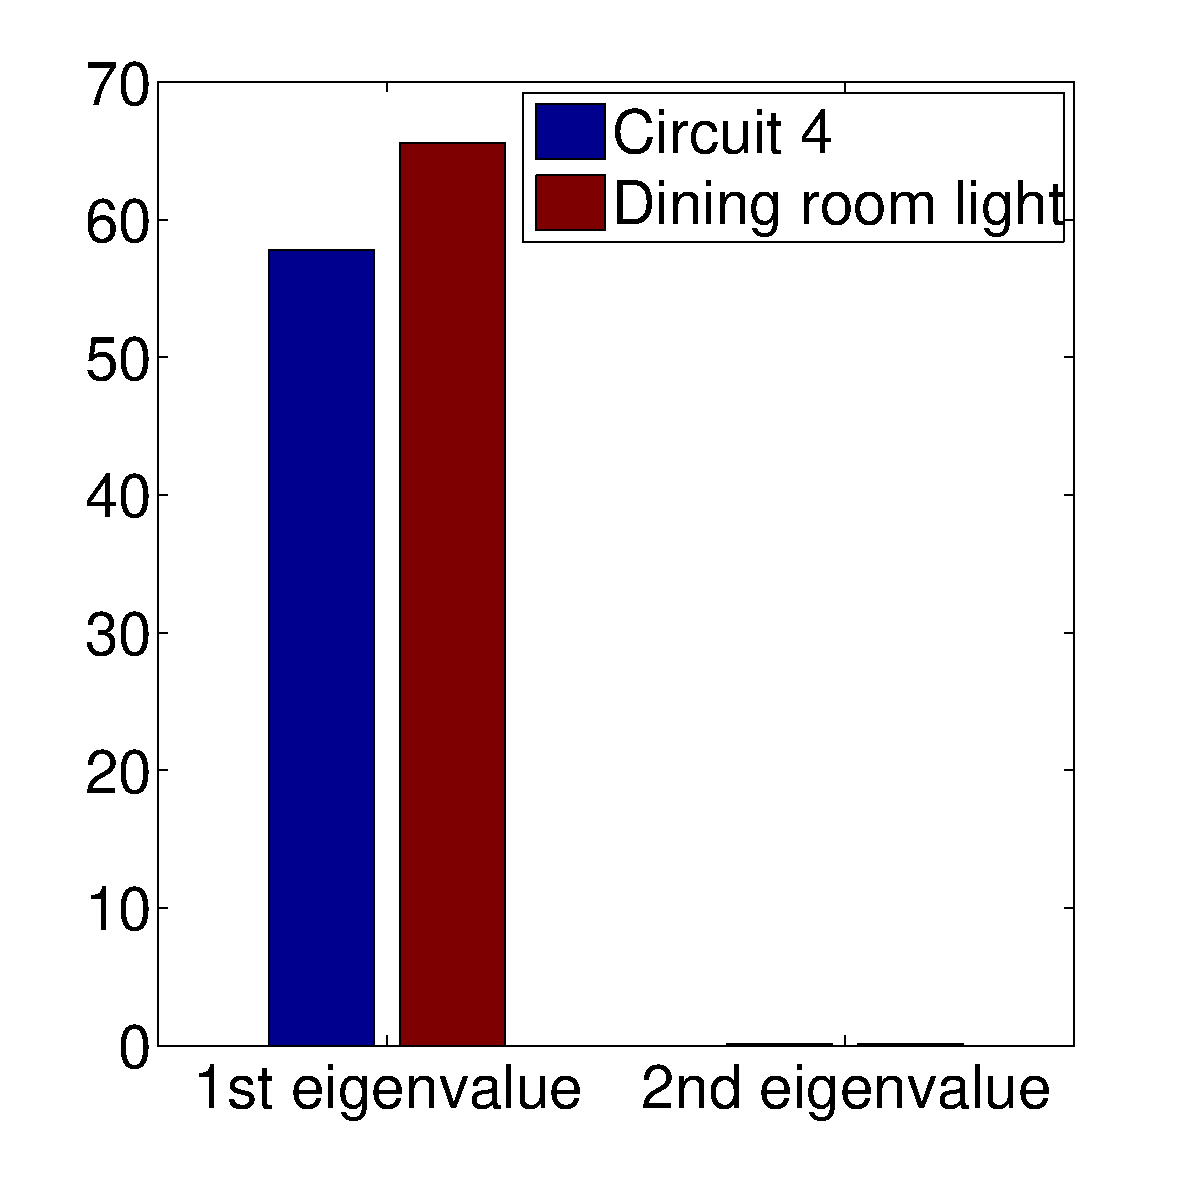
\includegraphics[width=0.3\textwidth]{figs/EigenValuesDevices.pdf}
	\caption{The eigenvalue of a circuit and dining room light. }
	\label{fig_eigenValue}
\end{figure*}


\textit{Harmonics:}
Harmonics constitute another class of features
defined over current or voltage waveforms.
Harmonics are integer multiples of the fundamental frequency of the waveforms. 
%\manishc{but what are harmonics? could you describe that in a senetnce or two?} \huijuanc{done.}
They are generated by non-linear devices such as VSDs,
electronic ballasts for fluorescent lighting,
switching power supplies, or rectifiers
when these devices start up or after they are on.
These waveforms are distorted to
be non-sinusoidal thus reflecting the inherent characteristics
of devices.
They play an important role in helping distinguish devices
when two devices share the same real power and reactive power. 
Harmonics can only be obtained from high frequency 
 data. 
%Equation (\ref{eq_harmonicsRange}).
%\begin{equation}
%\label{eq_harmonicsRange}
%f < N_{highest} \times 1/60 Hz
%\end{equation}

Figure~\ref{fig_harmonicsFeature} (a) and (b) illustrate the fact that, 
while an air compressor and refrigerator have similar real power,
by analyzing the first three harmonics
they can be distinguished.
Here, the magnitude of the first harmonic of air compressor is larger than 
that of the refrigerator. 
Also, the magnitude of the second harmonic of air compressor is smaller than 
the magnitude of the second harmonic of the refrigerator. 
\begin{figure*}[h]
\centering{
    \begin{tabular}{ccc}	
	
    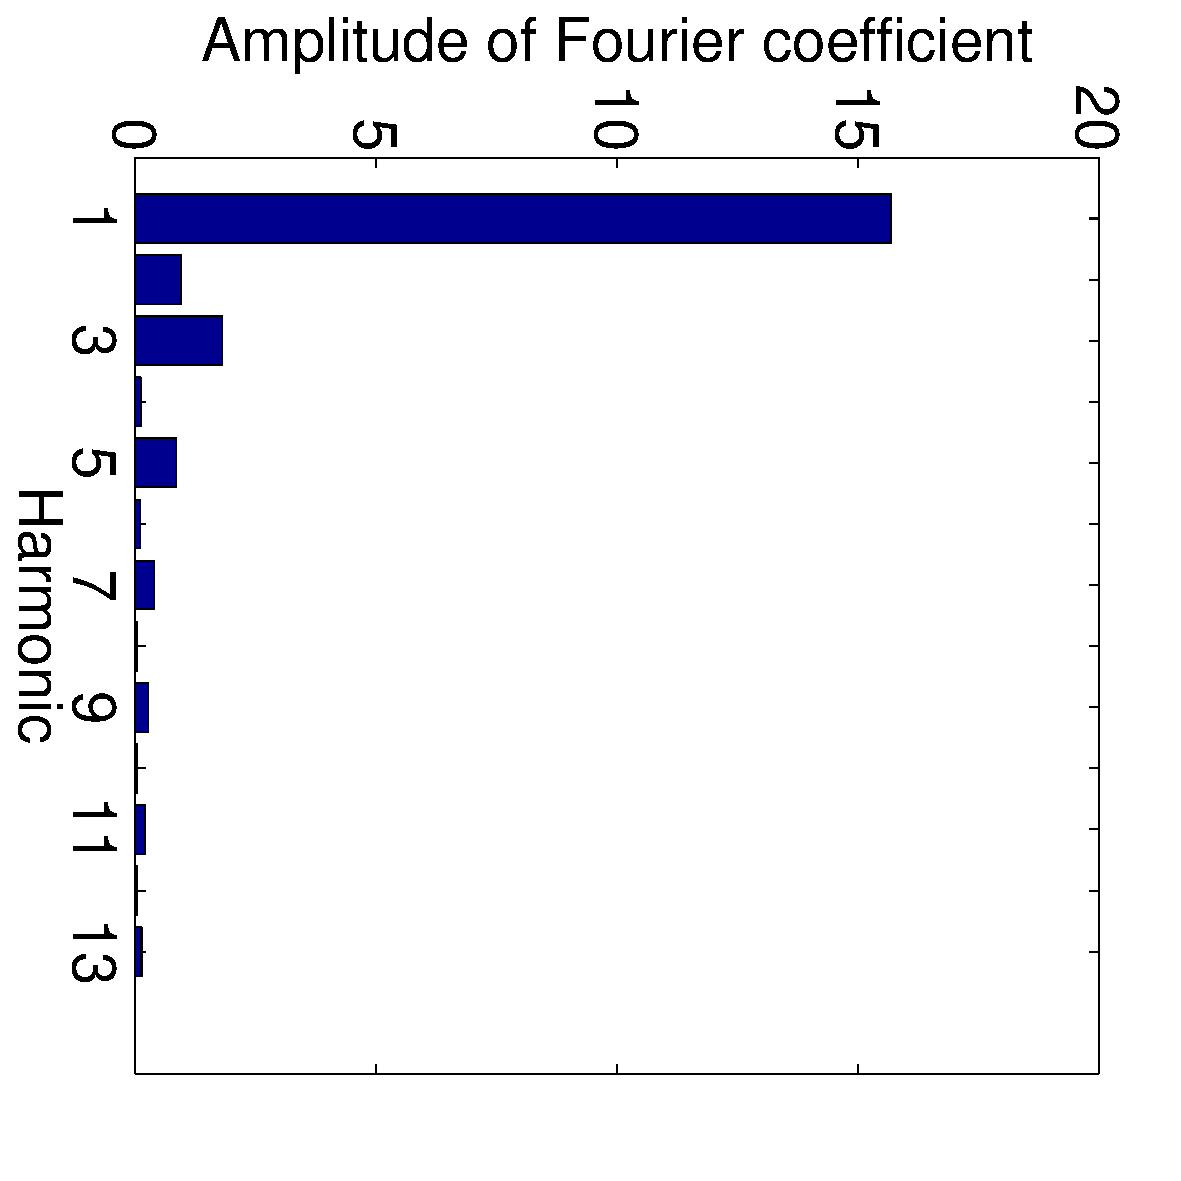
\includegraphics[width=0.33\textwidth,angle=90]{figs/refrigeratorTransientFFT.pdf} \hspace{1em}&
    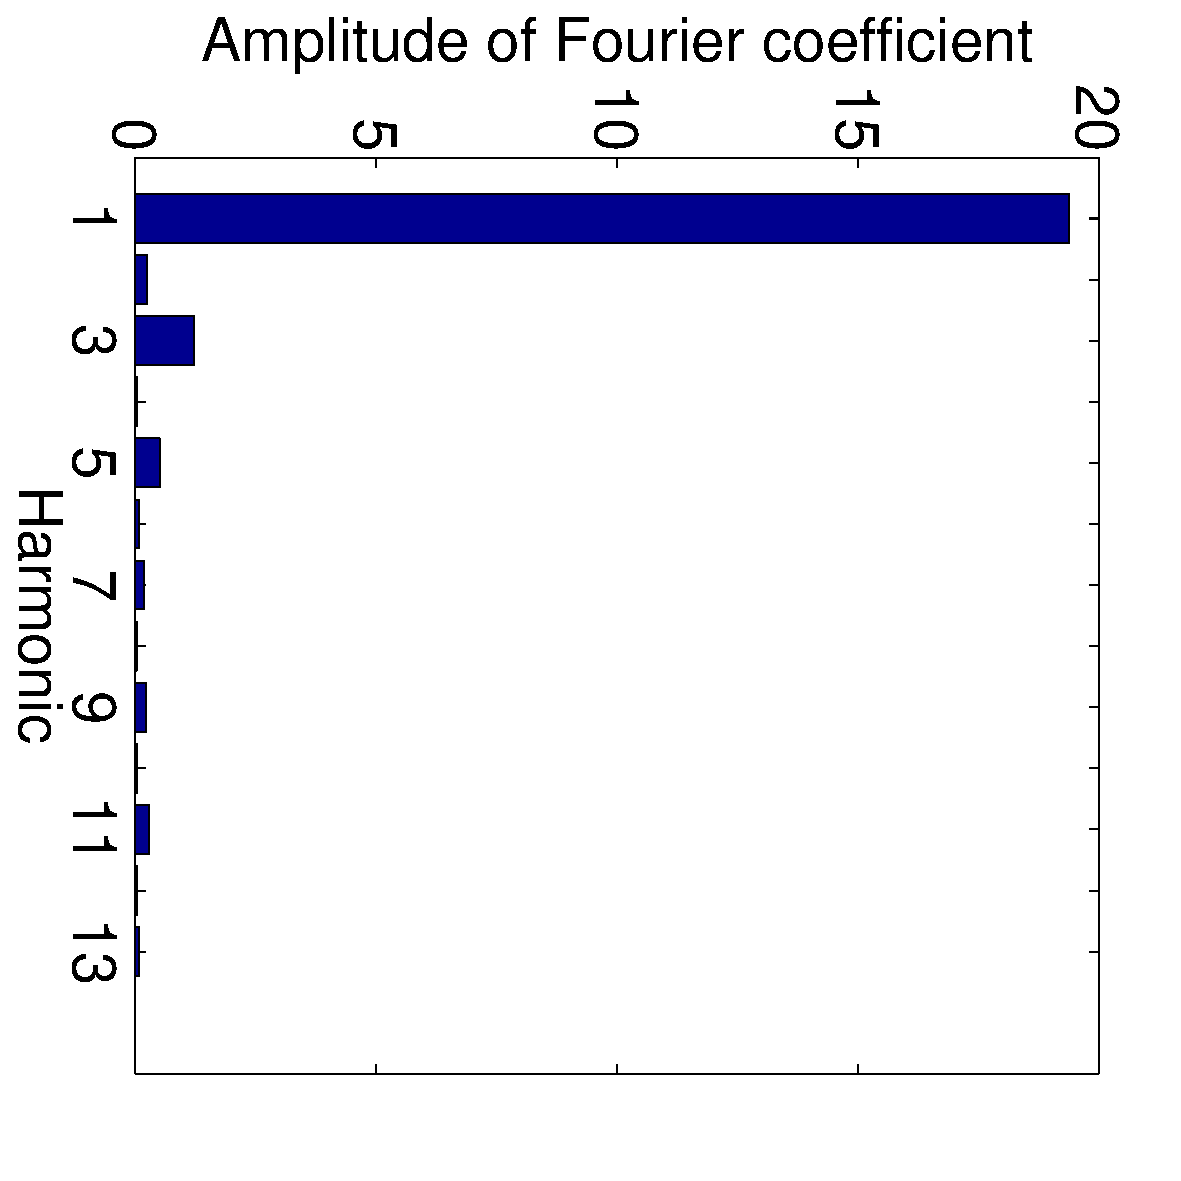
\includegraphics[width=0.33\textwidth,angle=90]{figs/airCompressorTransientFFT.pdf} \hspace{1em}&
    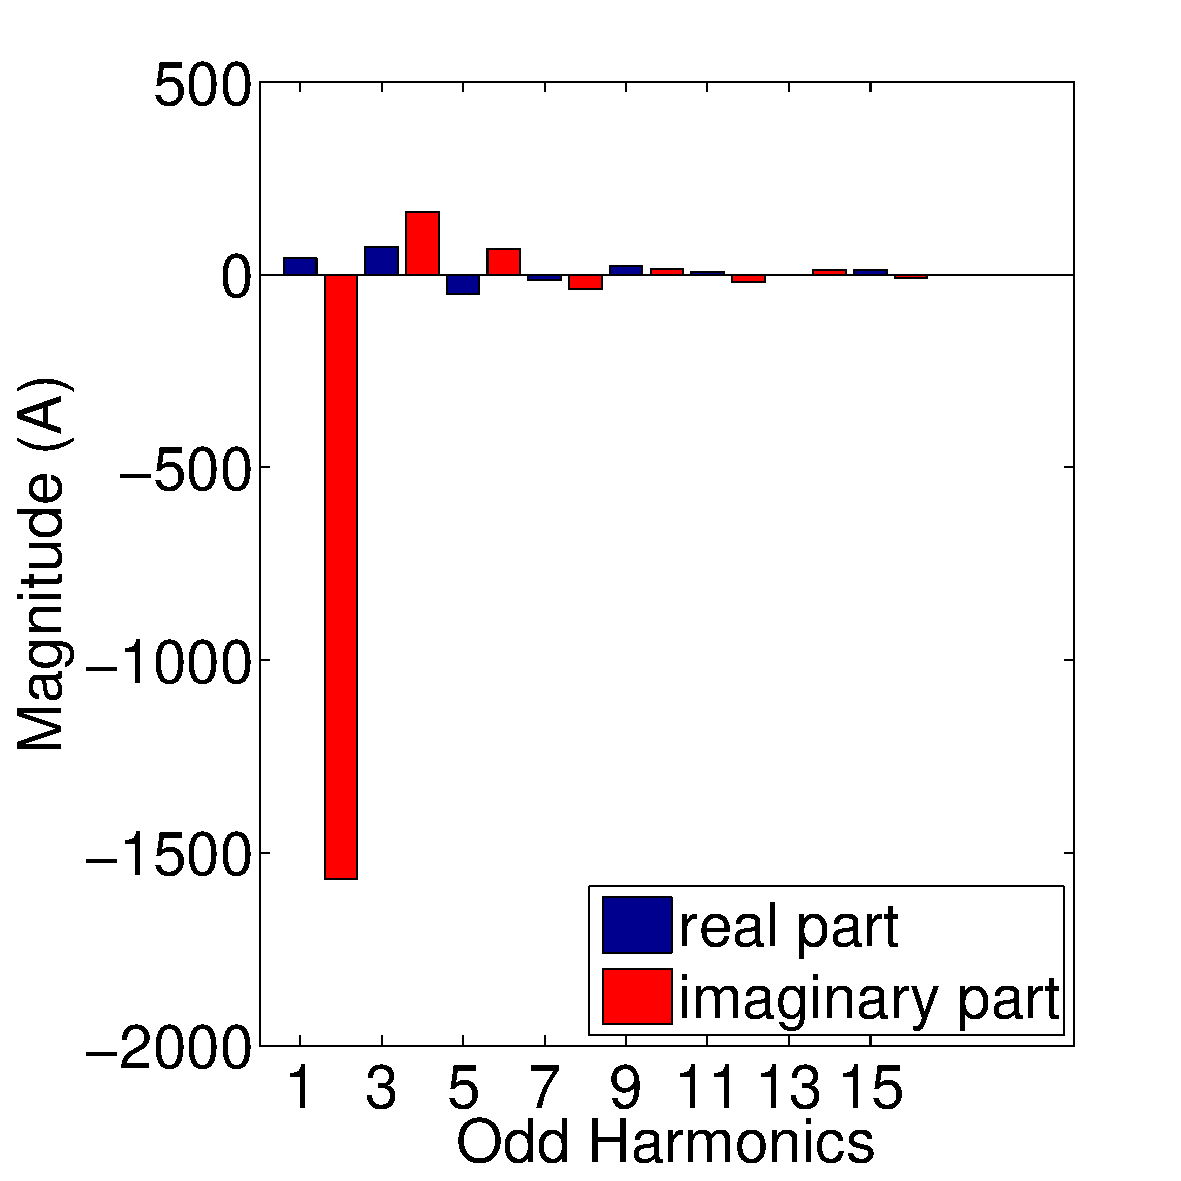
\includegraphics[width=0.33\textwidth]{figs/realImagHarmonicsRefrigerator.pdf} \tabularnewline
    (a) & (b) & (c) \tabularnewline
    \end{tabular}
    }
	\caption{Harmonics Feature of (a) a refrigerator and (b) an air compressor (c) real and imaginary part of odd number of harmonics of a refrigerator. }
	\label{fig_harmonicsFeature}
\end{figure*}


Harmonics have been employed in prior work 
\cite{laughman2003power,lee2005estimation,srinivasan2006neural,akbar2007modified,matthews2008auto,wichakool2009modeling}.
\iffalse
\huijuanc{will be deleted until huijuan's next comments.}
Some paper mentioned $N_{highest}$ as 11
because that's the highest useful harmonic for disaggregation.
\manishc{why?}.
Other papers~\cite{srinivasan2006neural} set $N$ to be 16 in order to capture more harmonics information
\manishc{but the previous senstence says that 11 is the highest useful harmonic}.
\huijuanc{change above sentences as follows.}
\fi
Generally only the odd harmonics are utilized. 
To the best of our knowledge, the highest employed harmonics are 
the 15 odd harmonics~\cite{srinivasan2006neural}. 
VSDs are hard to distinguish
but harmonics can be used to separate them. 
\iffalse
\huijuanc{delete until next comments of huijuan}
\cite{lee2003PhdThesis,lee2005estimation} thoroughly explained the approaches
as estimating the mean of higher harmonics of apparent power, 
then correlating the apparent power with the fundamental harmonic powers, 
thus identifying the VSDs \manishc{it is hard to understand this sentence,
  what is fundamental powers?  please re-word}
  \huijuanc{paraphrases as follows.}
 \fi
  \cite{lee2003PhdThesis,lee2005estimation} discovered that any VSD generates 
  a unique high harmonic power, which is identical among devices and effective for disaggregation. 
  Applying Gaussian random process to the power usage of VSD, 
  the $kth$ apparent harmonic power
  is calculated as $A_k=\sqrt{P_k^2+Q_k^2}$, where $k$ is the order number of 
the harmonics. 
The correlation pattern between the real power and 
the $kth$ apparent harmonic power is detected as a characteristic of each VSD. 

The real and imaginary parts of harmonics are also separately usable as features. 
Again, we only use the odd harmonics. 
The real part is calculated as 
$x_n=I_{(\frac{n+1}{2})}cos\theta_{(\frac{n+1}{2})}$ when $n$ is odd; 
%\manishc{how is the real part computed when n is even}\huijuanc{we only concern on the odd harmonics.}
the imaginary part is calculated as 
$x_n=I_{\frac{n}{2}}sin\theta_{\frac{n}{2}}$, 
for $n$ as even numbers, 
where $I_n$ is the magnitude of the $n$th current harmonic and
$\theta_n$ is the phase angle of the $n$th current harmonic. 
\iffalse
\manishc{are these equations only for odd harmonics? i vaguely remember that
  only odd harmonics are interesting. could you verify that, and find out why
  it is so, and include it here.}
  \huijuanc{Yes. That's the reason the paper of Srinivasan only mentioned the odd number of harmonics here.}
\fi
Figure~\ref{fig_harmonicsFeature} (c) shows the real part and imaginary part 
of the odd harmonics of a refrigerator. 
Also,~\cite{srinivasan2006neural} gives an example of how to separate devices 
by the real and imaginary part of harmonics. 

A variant of harmonics is the spectral envelope. 
This is a short-time average of harmonics 
and was proposed as a device feature in~\cite{leeb1995transient,laughman2003power}.
Further, harmonics can be used in conjunction with other features to disaggregate devices. 
\cite{wichakool2009modeling} introduces a switching-function 
to identify variable speed devices. 
\iffalse
\manishc{you use VSD in a lot of places,
  could you use the full expansion when it is used the first time, and then
  use VSD}\huijuanc{VSD has been explained in page 5. Is it necessary for us to list 
  all the abbreviations before the introduction section?}. 
\fi  
\begin{figure}[h]
\centering
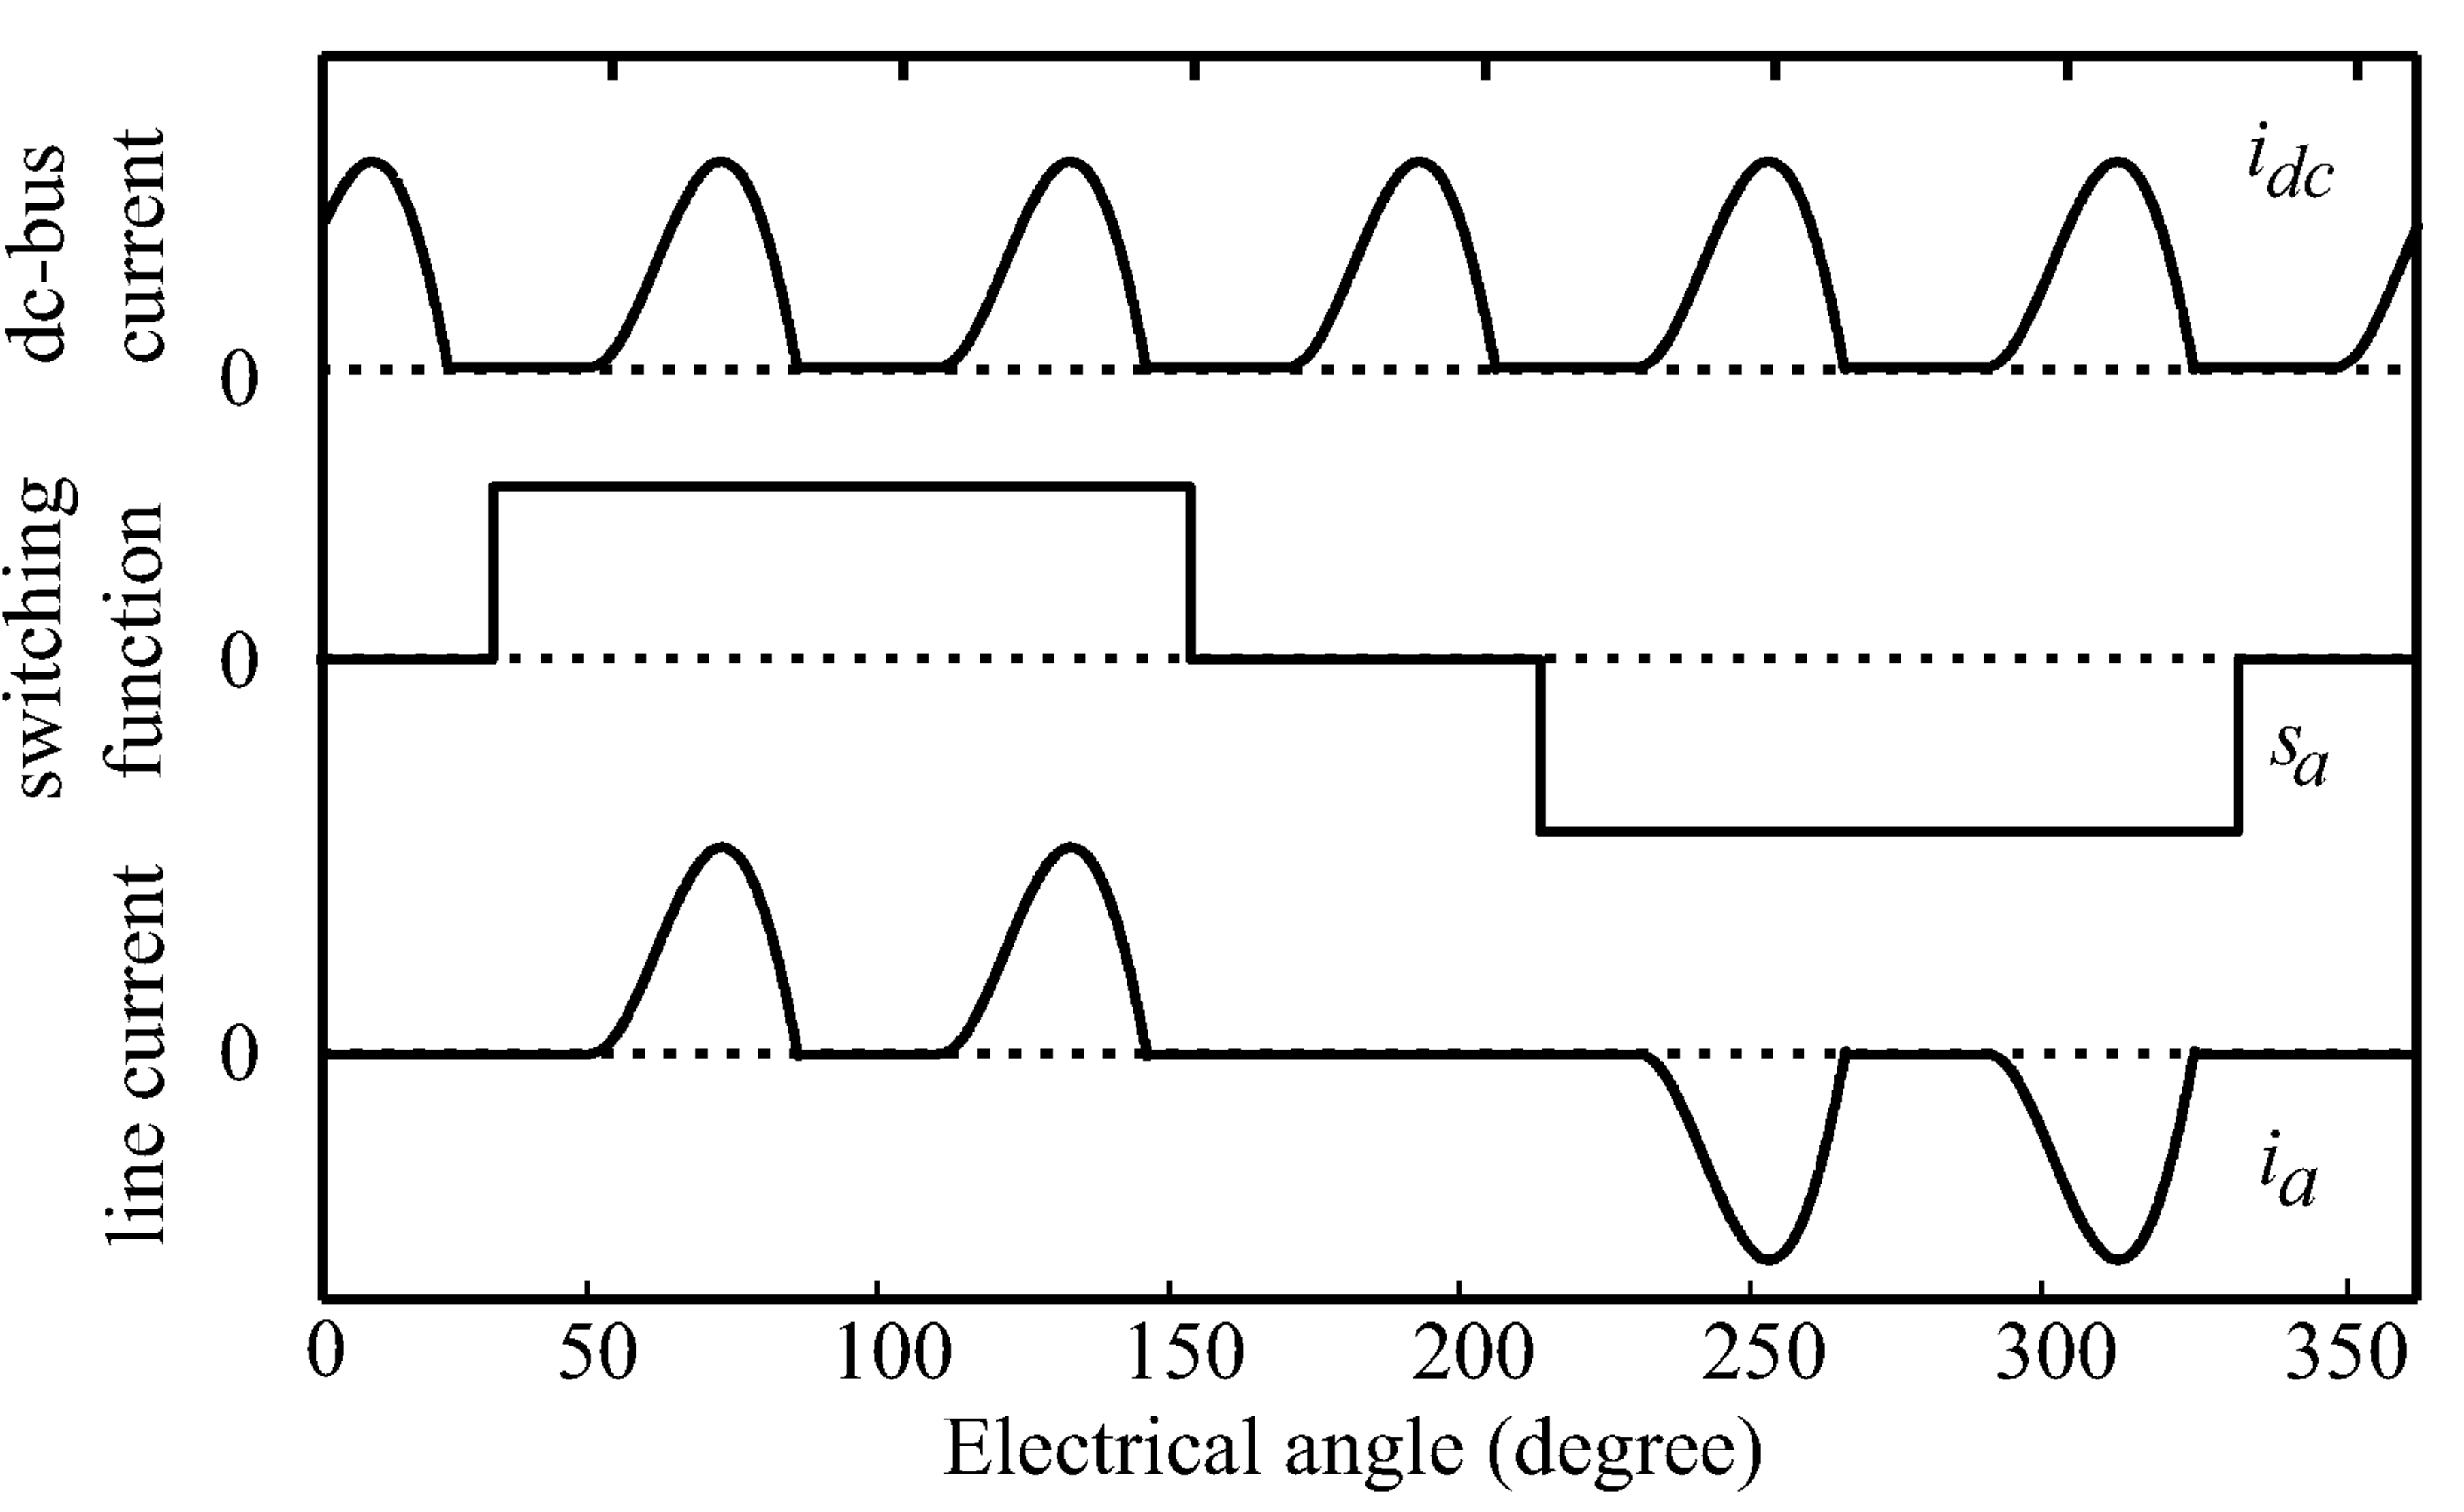
\includegraphics[width=0.5\textwidth]{figs/switchingFunction.png}
\caption{Switching-function for VSDs disaggregation (Courtesy:\cite{wichakool2009modeling}).}
\label{fig_switchingfun}
\end{figure}

Figure~\ref{fig_switchingfun} gives a comparison example
of current before and after rectifier and inverter of VSDs.
The operations of the rectifier of a VSD correspond to
a switching function.
The current is initially direct current $I_{dc}$ and
after the current goes through the switching process,
it changes to $I_a$.
The relationship between these two currents
is captured as $I_a(\theta)=S_a(\theta)I_{dc}(\theta)$, 
where $S_a(\theta)$ is the switching function. 
This switching function can be represented as 
a linear combination of different harmonics: 
$S_a(\theta)=S_0+\sum_n(S_n^p \sin n\theta - S_n^q \cos n\theta)$, 
where $n$ is the harmonic number, $S_0$ is the DC component,
and the variables $S_n^p$ and $S_n^q$ are the magnitudes of
the in-phase and quadrature parts of $nth$ harmonics of the
switching function. 
By comparing the Fourier coefficients with the $S_n^p$ and $S_n^q$ of harmonic coefficients,
these VSDs can be recognized.

\textit{Noise data:}
\cite{patel2007flick} and~\cite{gupta2010electrisense} recorded 
noise data instead of the current or voltage data.
Interestingly, this noise data
which occurs during switching on or off, 
can be used to identify devices
because different devices have different noise signatures. 
The frequency of the noise data is also treated as a feature. 
\cite{patel2007flick} first detects that noise is generated 
when a device in a residential building
turns on or off, or during the on state. 
With the introduction of switch mode power supplies (SMPS), 
the EMI generated by SMPS has also been
considered
as a feature~\cite{gupta2010electrisense}.
Figure~\ref{fig_LCDTVNoise} (a) depicts
the frequency generated by an LCD TV's on and
off events from
the Kaggle dataset~\cite{kaggle2013energy}.
Figure~\ref{fig_LCDTVNoise} (a) illustrates the noise time series background in red and 
the noise time series with newly added noise in blue. 
Figure~\ref{fig_LCDTVNoise} (b) shows that the newly added noise is segmented. 
By analyzing the mean value and standard deviation of the segmented noise, 
SMPS devices can be identified. 
\begin{figure}[ht]
\centering{
    \begin{tabular}{cc}	
	
    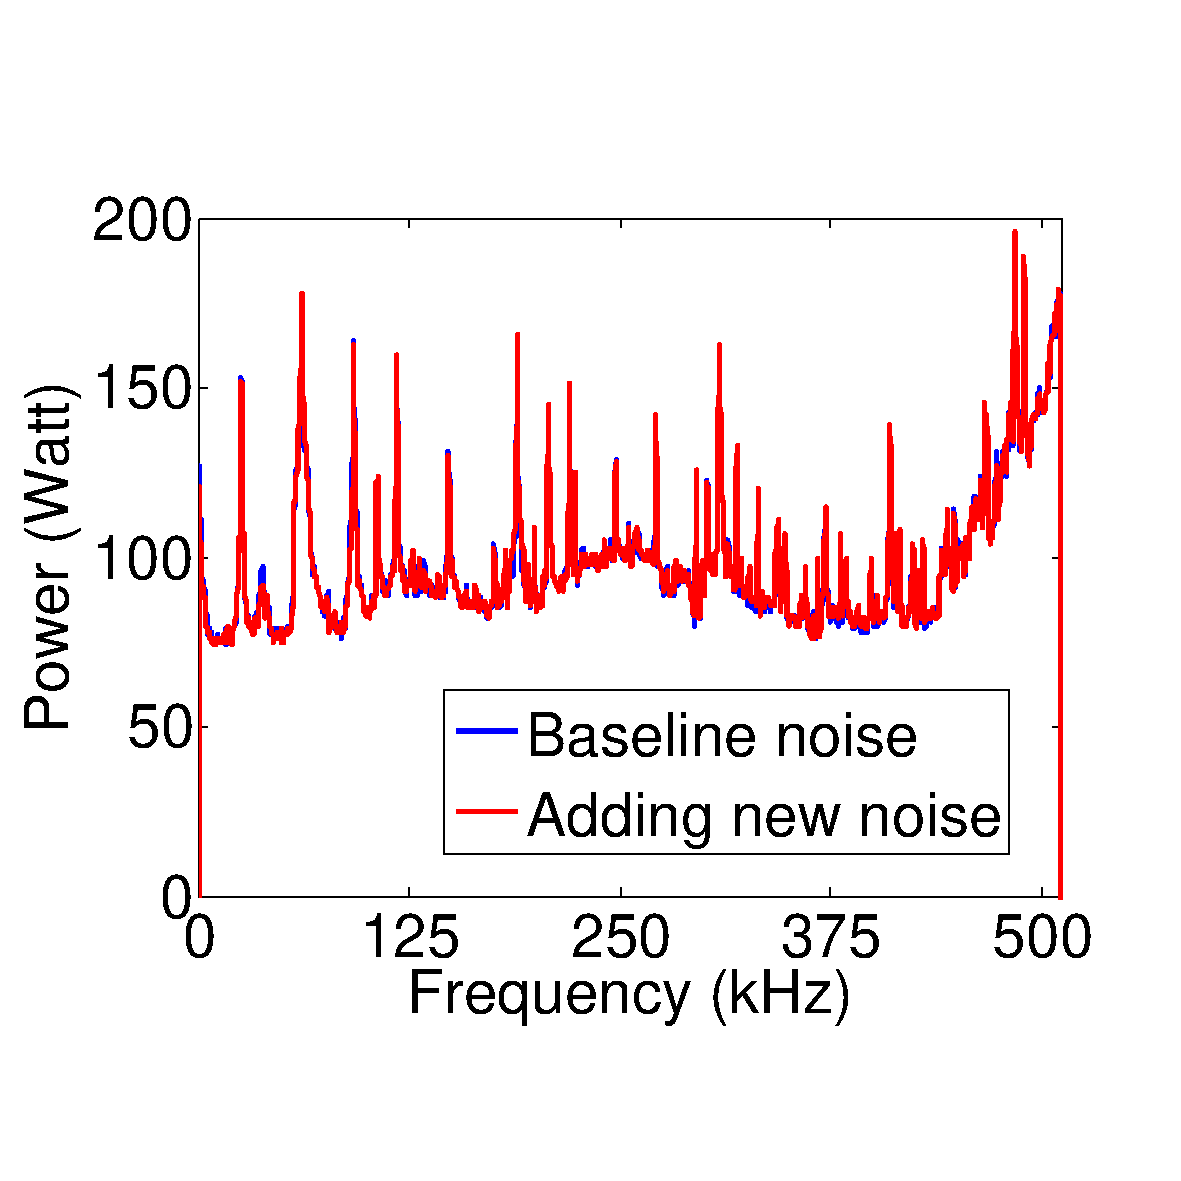
\includegraphics[width=0.5\textwidth]{figs/noiseMasterLCDTV.pdf} \hspace{1em}&
   % 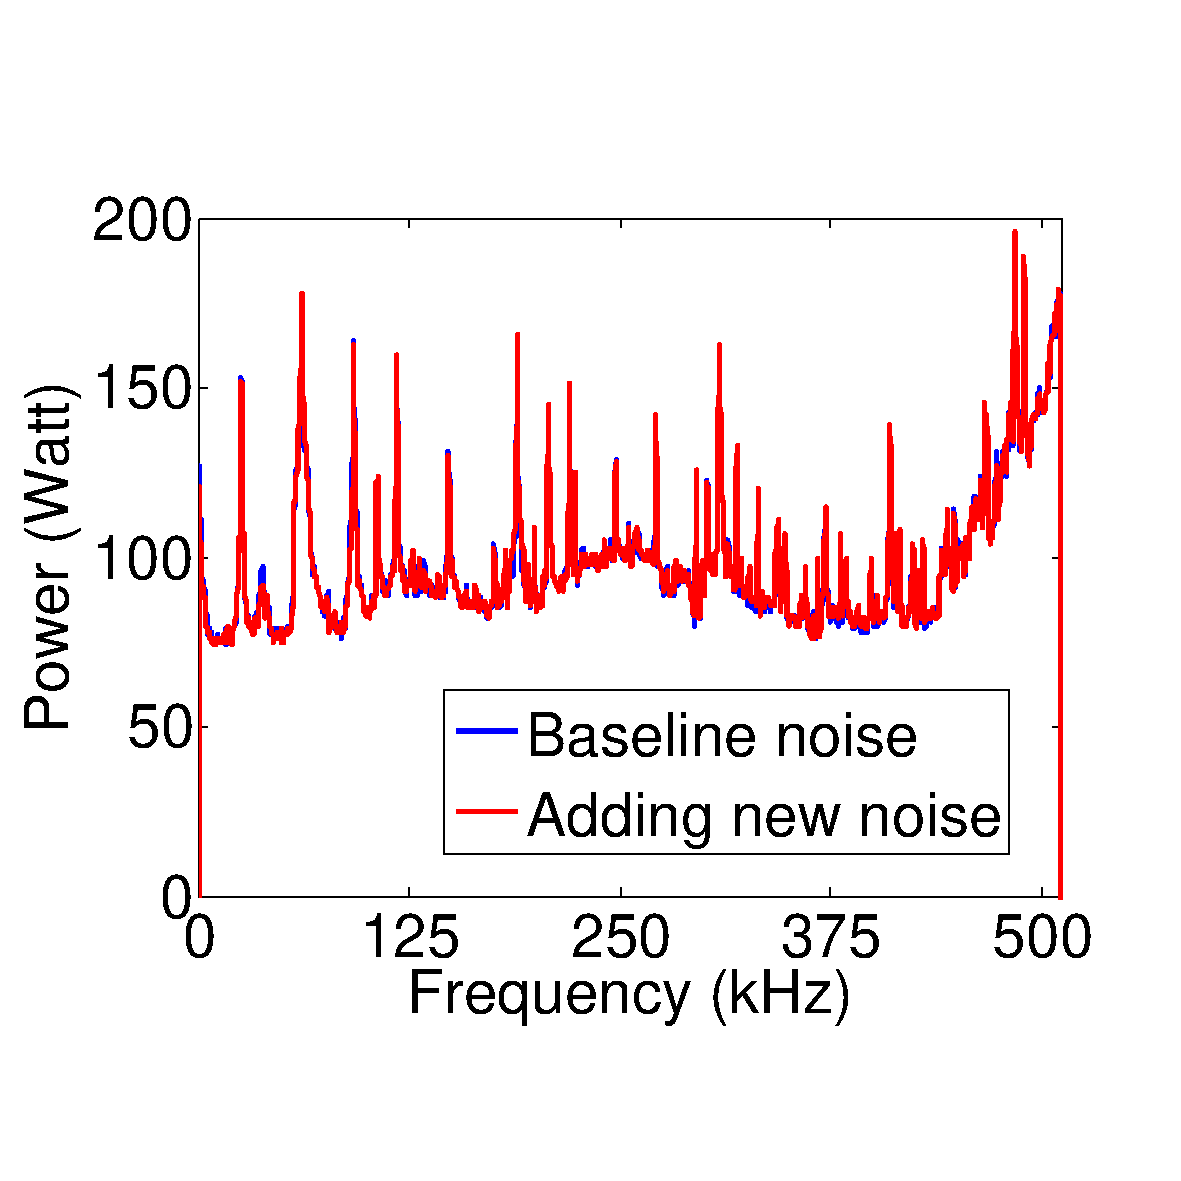
\includegraphics[width=0.3\textwidth,height=0.23\textheight]{figs/noiseMasterLCDTV.pdf} \hspace{1em}&
    \includegraphics[width=0.5\textwidth]{figs/noiseFeatureMasterLCDTV.pdf} \tabularnewline
    (a) &(b) \tabularnewline 
    \end{tabular}
    }
\caption{(a) Baseline noise with newly added noise. (b) Noise Feature of a device.}
\label{fig_LCDTVNoise}
\end{figure}
 

%\manishc{can you increase the font size of the text in fig 17, it is hard to read}\huijuanc{done.}

\subsection{Features beyond Current and Voltage}
%Besides AC-power values related to current and voltage,
%there are also additional features,
%such as time features,
%correlation between devices,
%electromagnetic field (EMF) emitted by devices,
%and etc.

\textit{Duration or time of use}
The operation of a device may conform to
a routine schedule of
when it is turned on or off,
and how long it is on or off.
The time of device usage involves the
month of the year, day of the month, day of week, time of the day,
and season of the year.
Generally, fans and air-conditioners
work in the summer and heaters work in the winter.
Figure~\ref{fig_timeofday} shows 
the total power usage of a commercial building~\cite{shao2013temporal}.
%\manishc{fig 18 caption should read 'day of week ...'}\huijuanc{done.}
Power usage is high during a weekday. 
In contrast, the power usage on weekends is quite low. 
\begin{figure*}[h]
	\centering{
    \begin{tabular}{c}	
	\includegraphics[width=0.3\textwidth]{figs/timeofday.pdf}
	%\includegraphics[width=0.3\textwidth,height=0.3\textheight]{figs/onduration_kim2010unsupervised.png} \hspace{1em}&
%    \includegraphics[width=0.5\textwidth]{figs/coefficients_kim2010unsupervised.png} \tabularnewline
   % (a) & (b) \tabularnewline
    \end{tabular}
    }
	\caption{Day of Week of Feature.}
	\label{fig_timeofday}
\end{figure*}


Date, time, and week features have been used in previous work.
For example,~\cite{kim2011unsupervised} points out that
a laptop is often powered-on in the morning of workdays
and that the TV is powered on during the evenings and weekends. 
Also,~\cite{kim2011unsupervised} analyze the on/off
distribution of devices and find that
they conform to a Gamma distribution.

\textit{Device correlation}
Some devices may need to operate with other devices.
For example, the TV and Xbox usually turn on and off
together.
Such correlation between devices has been
analyzed and integrated with a HMM-based model~\cite{kim2011unsupervised}.
This study calculates all the correlation coefficients and 
shows that 
both the correlation between TV and stereo
and the correlation between XBox and TV were as strong as 0.8.
\cite{chen2013novel} combines the features of on/off time, duration, and the correlations 
among devices to mine for usage patterns. This approach is 
designed especially for 
correlations between different 
types of devices other than the devices of the same type. 
In continuing work,~\cite{chen2014mining} develop an algorithm (CoMiner) to discover 
correlation between devices. 

\textit{EMF, sound, and light.}
Electromagnetic fields (EMFs)
are generated by electrical devices
when they are powered on.
Different devices can result in different EMFs which
can be monitored by an EMF sensor around devices.
This idea is used in~\cite{giri_study_2012}
to detect on/off state changes of devices.
In addition, sound and light resulting from
devices can help judge the status
of devices as described in~\cite{kim2009viridiscope}.
This work monitors sound by an acoustic sensor 
at 4Hz sampling rate
to identify the compressor status of a refrigerator. 
Also, the light intensity from a sensor installed in a refrigerator reflects 
whether the door is open or closed.

%%delete too long, unnecessary
%Figure\ref{fig_soundLightFeature} (a) 
%illustrates how sound measured by an acoustic sensor 
%identifies the compressor status of a refrigerator. 
%It shows that an acoustic sensor at 4 Hz sampling rate can detect the
%on/off status of the compressor.
%Figure\ref{fig_soundLightFeature} (b) 
%depicts the case that a light inside 
%a refrigerator monitors whether the 
%door opens or shuts. 
%It shows that light intensity in a refrigerator goes up when the door is
%open and the inside light is on.
%\begin{figure*}[ht]
	\centering{
    \begin{tabular}{cc}	
	\includegraphics[width=0.5\textwidth]{figs/kim2009viridiscope_sound.pdf} \hspace{1em}&
    \includegraphics[width=0.5\textwidth]{figs/kim2009viridiscope_light.pdf} \tabularnewline
    (a) & (b) \tabularnewline
    \end{tabular}
    }
	\caption{(a) compressor detection by acoustic sensor and (b) refrigerator detection by light. (courtesy: \cite{kim2009viridiscope}).}
	\label{fig_soundLightFeature}
\end{figure*}



\textit{Weather.}
Weather is a key factor for a commercial building's power usage
because of variation in the usage of the HVAC system in the summer and winter.
The correlation between temperature and electricity usage 
is studied in~\cite{pardo2002temperature}. 
%Figure \ref{fig_pardo2002temperature_temp} shows that, 
This work exploits the fact that
when the temperature is higher, 
the daily electricity usage increases. 
%\begin{figure}[ht]
%\centering
%\includegraphics[width=3 in]{figs/pardo2002temperature_temp.pdf}
%\caption{Variation of the total daily electricity load in Spain with the temperature index in 1998
%(courtesy: \cite{pardo2002temperature}).}
%\label{fig_pardo2002temperature_temp}
%\end{figure}

\textit{Other possible features.}
Additional sensors, such as motion sensors~\cite{cook2011sensor}, 
can determine activity inside a building, and provide useful input to a
disaggregation model.
\cite{srinivasan2013fixturefinder} integrates data from electricity 
and other sensors at home to disaggregate  low-power 
devices such as lightbulbs. \cite{wu2012low} proposes using plug-in low-cost outlet sensors to help capture 
appliance state. 
Also, ~\cite{uttama2013sustainable} uses limited plug-level sensors to improve 
disaggregation accuracy. 
In the future, more sensors are likely to be available and could be leveraged for 
energy disaggregation.

%Other factors like price may play a role.
%When the electricity price increases,
%people resort to other energy instead of electricity.

%idea: to be used in future research, not mention it in this paper?

%Low frequency data means the current/voltage
%waveform cannot be recovered by the sampling data.
%High frequency data refers to those data
%from which the current or voltage can be reconstructed.
%%and can be obtained from both
%low frequency and high frequency recorded data.
%However normally reactive is Not logged by reactive
%power meter because the cost of
%reactive power meter is high thus not used in
%energy disaggregation.
%Even though, reactive power and power factor
%can still be calculated by calculating the
%voltage and current values from the high
%frequency data, which can recover the
%voltage and current waveform.


%%%%%%%%%%%%
%For any circuit, we can classify the current and
%voltage response as the sum of a transient response
%and a steady response.
%For any voltage or current as a function of time,
%it can be written in form of
%\begin{equation}
%x(t)= x_T(t)+x_{SS}
%\end{equation}
%page 192 in book \cite{courtesy: eebook1}
%where $x(t)$ can represent both current and voltage.
%$x_{T}(t)$ is the transient state and
%$x_{T}(t)=(x_0-\tau F)e^{-\frac{t}{\tau}}$.
%$x_{SS}$ denotes the steady state.
%%%%%%%%%%%%%%%%%%%%%


%\section{Identifying Devices by Algorithms}
\section{Disaggregation Algorithms}
\label{sec:algorithms}
In most cases, before energy disaggregation algorithms can be applied, a
pre-processing phase is
necessary, which comprises its own set of algorithms.  
This phase extracts features or transforms data
from one domain to another, for example from the time domain to the frequency domain.
In this section, we first introduce pre-processing algorithms,  
then give an overview of all disaggregation algorithms (supervised, unsupervised, semi-supervised), 
and finally present the algorithms' advantages and disadvantages. 

\subsection{Pre-processing Stages}
\subsubsection{Event types}
While conducting energy disaggregation, the events in a time series play an important part in identifying devices.
These events can be classified into two categories; {\em point event} or
{\em vector event}.
\begin{enumerate}
\item{\textit{Point event}}. 
A point event is defined as an event that is determined by a single value from the input dataset, and 
this event is used to characterize a device.
%If an individual data instance corresponding to an event is used to judge a device, 
Examples of point events include real power, reactive power, or
power noise at any particular time. %  in a low frequency dataset. 

\item{\textit{Vector event}}. 
A vector event is defined as an event that is composed of several data points that characterize a device,
instead of just one data point. 
For instance, the waveform of current or voltage is a vector event.
When using vector events, if the raw data is transformed from the time domain to the frequency domain, 
the extracted features are also treated as vector events. It is common practice for current and voltage to be transformed into harmonics and 
wavelets. These transformations are best captured as vector
events.
\end{enumerate}

\subsubsection{Feature extraction algorithms}
Point events are easily obtained from the raw dataset, which may provide real power or reactive power as a time series. 
A commonly used event definition is to rely
on the difference between two successive data points.
%We calculate the difference between the current value and the previous value to obtain event information. 
%we can calculate the difference between the current and previous real power.
If the difference is significant (above a threshold), a point event is generated. Otherwise, no event is recorded. 
%Similarly, the reactive power event changes are easily obtained. 

Since high-frequency datasets provide rich information; it is quite common to extract vector events from them. 
After pre-processing a time series from the high-frequency data, 
we can obtain several features, like the startup value of the current, the current waveform, the harmonics of the current, 
the current transformation, the eigenvalue of the current, 
the voltage waveform, or voltage noises. 
Generally these pre-processing algorithms are classified into 
three types: 
{\em 1) Basic signal processing, 2) Fourier transforms, and 3) 
Wavelet transforms.}
Basic signal processing is used to filter, shift or amplify time series data. 
%Given a time series data, basic signal processing 
%operates to filter
%can be conducted the following operations,  to filter,  shift, or amplify. 
A Fourier transform converts the time-series data 
from the time domain to the frequency domain, and  
harmonics are acquired from the result of the Fourier transform.  
Wavelet transforms organize a time series into different 
scale components, and each component is assigned to a frequency range. 
Features extracted in this manner
by the wavelet transform are relatively stable.  
For instance, when a device is turned on, a corresponding sharp peak is generated 
in the time domain which is not characteristic of the device's power signature. 
However, the use of wavelet transformation in the frequency domain will discard this transient information and be more consistent with the device's actual power signature.

%Wavelet has the advantage of
%not being influenced by sharp peaks which appear when some devices are turned on. 
%To extract the features or attribute of electrical devices,
%some algorithms have been researched in feature selection
%as shown in .
%% to be updated ???
\begin{table}[h]%
\caption{Pre-processing algorithms with vector event feature extraction. }
\label{tab_featureAlg}
\begin{center}
\makebox[\textwidth]{
\begin{tabular} {|l|l|l|l|l|l|l|l|}
\hline
Feature-identification Algorithm  & \rotatebox{90} {Startup of $I_{AC}$} & \rotatebox{90} {Harmonics of $|I_{AC}|$} &\rotatebox{90}{ $I_{AC}$}  & \rotatebox{90}{$I_{AC}$ transformation} & \rotatebox{90} {eigenvalues of $I_{AC}$} & \rotatebox{90} {$V_{AC}$} & \rotatebox{90} {voltage noise }  \\
\hline
Signal Processing\cite{cox2006transient}&&&&&&$\surd$& \\
\hline
Fourier Transform \cite{wichakool2009modeling}&&$\surd$&$\surd$&&&&\\
%\hline
%Goodness-of-fit\cite{jin2011robust}&&&&&$\surd$&&&$\surd$&\\
\hline
Wavelet Transforms\cite{chan2000harmonics}&&&$\surd$&&$\surd$&&\\
\hline
\end{tabular}
}
\end{center}
\end{table}%

Table~\ref{tab_featureAlg} gives examples of several vector events using these 
three types of pre-processing algorithms.
Basic signal processing steps, a low-pass filter, amplification and shifting 
are used to extract the distorted voltage shapes in~\cite{cox2006transient}.
In~\cite{wichakool2009modeling}, the Fourier transform of the waveform is applied to 
find distinct coefficients for those VSDs. 
The Fourier transform is also used in~\cite{jin2011robust} to extract 
harmonic features. 
The wavelet transform is employed to identify harmonics features of devices 
in~\cite{chan2000harmonics}. 

\subsection{Overview of Disaggregation Algorithms}
As the number and complexity of the features used have increased, 
%As more and more features are extracted from the recorded data,
so has the complexity of the 
disaggregation algorithms.
%vary from simple
%to complex.
From a data mining perspective,
algorithms can be sorted into three categories:
supervised, unsupervised, and semi-supervised.
Table \ref{tab_algSummary} lists these three categories.
\begin{table}[h]%
\caption{Categories of energy disaggregation algorithms.}
\label{tab_algSummary}
\begin{center}
\makebox[\textwidth]{
\begin{tabular} {|l|l|l|l|l|}
\hline
Category & Sub-category&Algorithm Name & Example & Features Adopted  \\
\hline
\hline
\multirow{18}{*}{supervised}  & \multirow{12}{*}{Classification}&Pair-wise match & \cite{hart1992} & real reactive power \\
\cline{3-5}
&&Neural Network & \cite{roos1994using} & real power, reactive power \\
\cline{3-5}
& &SVM & \cite{patel2007flick} & startup of $I_{AC}$ and voltage noise \\
\cline{3-5}
& &SVM, AdaBoost, RBF, NN & \cite{onoda2000applying} & startup of $I_{AC}$ \\
\cline{3-5}
& &SVM, KSC & \cite{onoda2000applying2} & startup of $I_{AC}$ \\
\cline{3-5}
& &SVM, RBFN & \cite{nakano2007non} & real power, harmonics of $I_{AC}$ \\
\cline{3-5}
&&Bayesian Classifier & \cite{berges2010enhancing} & real power \\
\cline{3-5}
& &Genetic algorithm & \cite{baranski2004genetic} & startup of $I_{AC}$, on duration \\
\cline{3-5}
& &Rule-based & \cite{powers1991using} & real power \\
\cline{3-5}
& &Dynamic Bayesian network & \cite{froehlich2011disaggregated} & real power \\
\cline{3-5}
& &Decision Tree & \cite{berges2009learning} & startup of $I_{AC}$ \\
\cline{3-5}
& &AdaBoost & \cite{berges2009learning} & startup of $I_{AC}$ \\
\cline{2-5}
& \multirow{2}{*}{Nearest Neighbor}&KNN & \cite{shaw2000PhdThesis} & startup of $I_{AC}$ \\
\cline{3-5}
&& Duration PDF & \cite{zeifman2011viterbi} & real power, on duration \\
\cline{2-5}
& \multirow{1}{*}{Statistical Model}&General likelihood ratio & \cite{anderson2012event} & real reactive power, duration \\
\cline{2-5}
& \multirow{5}{*}{Optimization}& Dynamic Programming & \cite{baranski2004detecting} & $I_{AC}$ \\
\cline{3-5}
&& Dynamic Model & \cite{dong2013dynamical} & real power \\
\cline{3-5}
&& Integer Programming & \cite{suzuki2008nonintrusive} & $I_{AC}$ \\
\cline{3-5}
&&Sparse Coding & \cite{kolter2010sparse} & real power \\
\cline{3-5}
&& Nonnegative Tensor Factorization & \cite{figueiredo2014electrical} & real power \\
\hline
\hline
\multirow{5}{*}{unsupervised}  &\multirow{1}{*}{Clustering} & Hierarchical Clustering & \cite{gonccalves2011unsupervised} & real power, reactive power\\
\cline{2-5}
& \multirow{3}{*}{HMM-based}  &FHMM & \cite{kim2011unsupervised} & real power, time, duration\\
\cline{3-5}
& &AFAMAP & \cite{kolter2012aistat} & real power, startup of $I_{AC}$ \\
\cline{3-5}
& &Difference FHMM & \cite{parson2012nonintrusive}& real power \\
\cline{2-5}
&\multirow{1}{*}{Temporal mining}  & Motif Mining & \cite{shao2013temporal} & real power \\
\hline
\hline
\multirow{3}{*}{Semi-supervised}  & Clustering&Hierarchical Clustering & \cite{lam2007novel} & startup of $I_{AC}$, $I_{AC}$, $V_{AC}$ \\
\cline{2-5}
& HMM &HDP-HSMM & \cite{johnson2012bayesian} & real power \\
\cline{2-5}
& Optimization&Contextually supervised & \cite{wytock2014contextually} & real power \\
\hline
\end{tabular}
}
\end{center}
\end{table}


%So far, data mining algorithms focus on the
%low sampling frequency recorded data set.
%Optimization algorithms is employed on both high frequency
%and low frequency data set.
%Signal processing algorithms are mainly applied to
%the high sampling frequency recorded data.
%Figure\ref{fig_algFlowchart} describes the relationship of
%these three types of algorithms.
%Signal processing algorithms can run stand-alone to identify devices.
%Also, it can be integrated with data mining or optimization
%algorithms as the preprocessing part.
%Under the latter condition, usually the data is
%transformed from the time domain to frequency domain.
%\begin{figure}[ht]
%\centering
%\includegraphics[width=4in]{figs/algorithmsFlowchart.pdf}
%\caption{Algorithms Flowchart}
%\label{fig_algFlowchart}
%\end{figure}

%From an events perspective,
%all algorithms are classified into point-based algorithms
%or vector-based algorithms, as shown in the 
%last column of Table \ref{tab_algSummary} under the Features Adopted category.

%\manishc{the table doesn't show if those algorithms are point or event
%  based. Also, an algorithm could use both point and event features.}
%\huijuanc{change as the following sentence.}  
From an events perspective, 
algorithms can be point-based, vector-based or a combination of the two
strategies.
Point-based algorithms are dedicated to the processing of the turn-on and turn-off
events of devices. 
Vector-based algorithms treat the current, voltage or
power value as an ordered time series instead of
focusing on a single transition state. 
Point-based algorithms perform well on discrete steady-state
devices, but perform poorly on devices with vector features, 
such as variable speed devices (VSDs). 

%\textbf{Comparison of Supervised and Unsupervised Algorithms}
%\huijuanc{the following paragraph is added to compare the advantages and disadvantages of 
%supervised and unsupervised algorithms.}
I summarize the merits and shortcomings of supervised and 
unsupervised learning algorithms for disaggregation in terms of the installation cost of meters, dataset size requirements for building models, 
the computational cost of operation process, and the accuracy results of disaggregation. 
Compared to unsupervised learning approaches, the advantages of supervised learning algorithms are that the disaggregation accuracy is typically
higher (for the same dataset), they require smaller data sizes, and
have typically faster operation (in practice).
Compared to unsupervised learning algorithms, the main disadvantages of supervised learning techniques lie in that the labelled data of each device is difficult to obtain due to the cost of meter installation.

%\item The classification based techniques rely on the accuracy of  the extracted features of each device. 
%However these features  are hard to access in practice because of the meters that capture these measurements have a very high installation cost.


%To have a look at the algorithms and the features in detail,
%the major algorithms and the adopted features of each algorithm
%are listed in Table.\ref{tab_algorithms} in Appendix section.

%\subsection{Supervised Learning Algorithms}
\subsubsection{Classification-Based}
\label{sec:supervised}
%Supervised learning based energy disaggregation algorithms have been an area of research since %since this topic was first proposed by Hart~\cite{hart1992} and over the last couple of decades %significant progress has been made in this field. 
Supervised learning-based energy disaggregation algorithms focus on distinguishing devices from aggregated data 
%by training a model using data from another time period combined with data from each circuit/device.
%Essentially these algorithms 
by treating the problem as one of device classification.
%Some classification algorithms are utilized standalone,
%others combine several classification algorithms together.
These classification algorithms include
simple pair-wise matching, rule-based algorithms,
%KNN,
SVMs, kernel-based subspace classification,
Bayesian classifiers, neural networks,
genetic algorithms,
dynamic Bayesian networks,
sparse coding,
AdaBoost,
decision trees, and
combinations of techniques like SVM and AdaBoost.

%\subsubsubsection{Neural network}
\textbf{Neural networks}
%Algorithms using neural network essentially take a device feature classification approach to energy %disaggregation. 
%Neural network is adopted by several papers in energy disaggregation area
A basic energy disaggregation technique utilizing a neural network 
is implemented in two steps. 
First, in the training stage, a neural network is trained 
to learn several features of multiple devices. 
Second, in the test stage, each feature extracted from the aggregated data 
is provided as an input to the neural network. 
If the neural network recognizes the input by associating it with one of the features learned in the training phase, then the device that generated that input is classified accordingly. 
%for single feature over all features, 
%it's to compare the whether the error rate becomes the lowest. 

%For the purpose of testing, 10% or 20% deviation at one
%harmonic parameter (amplitude or phase angle) was
%applied to the harmonic content table of typical
%commercial area. The evaluation of the calculation results
%is compared with Percentage Relative Error (PRE):
%NA/CRefrigeratorr
%(%) = [
%( Pti − Pi ) 2 ]0.5
%i =1
%where N is the number of devices. Pti is the load i
%percentage calculated from ANN model and Pi is the
%actual percentage of load i.
A neural network example is 
illustrated in Figure~\ref{fig_neuralNetwork}. %, roos1994using, baranski2003nonintrusive}. 
There are $d$ features in the input and 
$M$ number of devices on the output. 
The neural network defines $K$ hidden states. 
\begin{figure}[h]
\centering
\includegraphics[width=3 in]{figs/neuralNetwork.pdf}
\caption{Neural Network Approach for Energy Disaggregation.}
\label{fig_neuralNetwork}
\end{figure}


Generally, the evaluation for a neural network-based classifier is 
to compare the relative error percentage.
%Neural network has the advantage over detect the interaction between
%the disaggregated features and ground truth
%but it works very slow.

%Several papers have adopted basic neural network for device classification. 
Roos et al. initially proposed to adopt
neural network classification for classification based on real
power and reactive power by 
transforming the aggregated data into images for processing~\cite{roos1994using}.
Next,~\cite{baranski2003nonintrusive} employs a backpropagation (BP)
neural network with the attributes of number of states,
duration time, and average energy consumption. %to identify devices.
Furthermore, 
the training stage of~\cite{duan2004neural} and~\cite{srinivasan2006neural} are based on the current waveform
and harmonics. %to extract signatures by Fourier transform thus identify devices.
The latter paper treats eight odd-numbered harmonics as a vector event feature 
for classification and chooses 16 hidden nodes.
Note that~\cite{srinivasan2006neural} compares several neural network approaches, 
namely multilayer perception (MLP), radial-basis function (RBF) network,
and support vector machine (SVM) with linear, polynomial and
RBF kernels.
The results suggest that MLP and RBF-based approaches have high classification accuracy. 

%neural network
Chang et al. extend the back propagation approach
by employing an electromagnetic transient program (EMTP) with
transient real power when devices start up~\cite{chang2008load2}. 
The transient shape is a vector event rather than a point event. 
To identify devices from aggregated data adaptively,
a window size %$\Delta t $ 
$w$
is adopted to enhance the algorithm
as an adaptive neural network. 
Initially, the differential values $dP_{transient}$ for period time %$\Delta t$ 
$w$
represent the characteristics of a class of devices. During the training process,
the time period value %$\Delta t$ 
$w$ increases by $\delta$ from $1$ to %$\Delta t$
$w$.
The $\delta$, which achieves the highest recognition accuracy, is retained.

Recently a basic adaptive neural network (ANN) applied to energy disaggregation was presented in ~\cite{liang2010load}. 
%The paper selects backpropagation ANN (BPANN) to
%train a model. 
Based on a combination of features,
such as real power, reactive power,
transient shapes, harmonics, the eigenvalue of the current waveform,
the voltage waveform, etc., 
this paper establishes a committee decision system based on 
three rules: most common occurrence (MCO), least unified residue (LUR), and
maximum-likelihood estimation (MLE), to classify devices. 
As a result, the disaggregation accuracy is high. 

%The system work flow is Figure\ref{fig_system_srinivasan2006neural}.
%In the first step, the distorted waveform generated by non-linear
%devices is transformed by Fourier analysis.
%\begin{figure}[h]
\centering
\includegraphics[width=3 in]{figs/system_srinivasan2006neural.pdf}
\caption{System for Neural Network (Courtesy:\cite{srinivasan2006neural})}
\label{fig_system_srinivasan2006neural}
\end{figure}


%Then the eight odd-numbered harmonics are extracted as vectors as
%illustrated. %in Figure\ref{fig_harmonics_srinivasan2006neural}.
%The real part and imaginary part are separated as the input of
%ANN.
%Since there are 8 devices, the output number of nodes is 8.
%The number of hidden nodes is chosen as 16.

Two variants of the basic neural network approach
have been proposed. %LVQ neural network
Reference \cite{yang2007design} classifies the transient events by way of
back propagation,  
and \cite{chang2008load} adopts learning vector quantization (LVQ) to
recognize devices. % combination with GA
Neural networks have also been combined with other approaches. For example,~\cite{chang2010newmethod} combines a multi-layer feed-forward neural network with a genetic algorithm to 
to analyze the device turn-on transient signatures. 
%%%%%%%%%%%%%%%end of neural network

%\subsubsubsection{Support vector machine}
\textbf{Support vector machines}
SVMs attack the problem using multiclass learning techniques by learning 
event features only from the training data, in contrast with unsupervised methods that learn
features from the entire dataset. 
%\manishc{that is in general true for all classifiers} \huijuanc{Yes. unsupervised disaggregation approaches learn the features from the entire dataset other than part of the dataset. I add unsupervised.}
Kernels such as the radial basis function (RBF) kernel are adopted to learn complex features like harmonics. At first, SVMs were employed to classify devices by 13 odd-order harmonic current 
and phase angles from on and off events~\cite{onoda2000applying}. 
Later, a kernel-based subspace classification (KSC) approach is used for 
events classification in SVM~\cite{onoda2000applying2}. 
%%% the following is needed or not? 10-08-2014
%The RBF kernel is introduced as Equation (\ref{eqn_rbfSubspace}). %for both KSC and SVM.
%\begin{equation}
%\label{eqn_rbfSubspace}
%k(x,y)=exp(\frac{{\lVert x-y \rVert}^2}{\sigma ^2})
%\end{equation}
%Where $x$ is the dimensional patterns,
%$y$ represents the classified devices,
%$k(x, y)$ is the kernel matrix. 
% and its $(i, j)$ element is $k(x_i, y_j)$.

SVMs were widely utilized with  noisy datasets although they
do not scale well for large data sets. 
%because 
%the size of these datasets is much larger than 
%that of AC power features and SVM has the ability to perform fast computations on
%large data sets. 
%\manishc{svm's don't scale well for large data sets}
%\huijuanc{SVM does scale for large data sets according to the following two references. "Classifying large data sets using SVMs with hierarchical clusters", "Making SVMs scalable to large data sets using hierarchical cluster indexing".}
%\huijuanc{delete the sentences related to scalability.}
An SVM was adopted by~\cite{patel2007flick}
to classify transient pulses noise from various homes.
%During processing, transient events from noise data are isolated and
%then the disaggregated events are classified into these transient events.
%The test is done for the residential buildings.
%The author figures out it could be applied to commercial buildings
%which may include more compound devices and complex noises.
In~\cite{froehlich2011disaggregated}, 
SVMs are applied to transient and continuous voltage noise data.
The noisy voltage generally produced by devices influences
the power wiring.
According to Gen Marubayashi~\cite{mambayashi1997noise},
there are three types of voltage noise:  
on-off transient noise;
steady-state line voltage noise, which is produced at $60$ Hz or
integer times of $60$ Hz (e.g. harmonics),
and steady-state continuous noise which is generated beyond
$60$ Hz.
Voltage noise data is sampled with very high frequency.
During pre-processing, the noisy recorded voltage data
is transformed by a Fourier analysis. 
Then, three to five transient voltage noise signatures are labeled
and a threshold is pre-defined.
During the training phase,
by sliding a window on the aggregated voltage noise,
a part of the data with continuous voltage noise
is extracted and compared with the pre-stored voltage noise data by measuring the
Euclidean distance.
If the distance is larger than the pre-defined
threshold, then the feature vector is exerted from
this window.
After sliding over aggregated voltage noise data,
all these feature vectors are classified
by the SVM.

In addition to their use
as a standalone classifier, SVMs are also utilized in energy disaggregation 
in combination with other approaches. 
In~\cite{nakano2007non}, 
both stand-alone SVMs and a combination of SVM and radial basis function network (RBFN)
are implemented to compare the disaggregated data with the ground truth harmonics.
%Then parameters for KSC and SVM are estimated and tested.
%The results shows that KSC performs with lower error rate
%for some devices and a bit higher error rate for other devices.
%However, the computation cost of KSC is much lower than SVM.

%Support vector machine is to find a large margin between
%two classes thus minimize the distances of each plate.
%Figure\ref{fig_svmClassifier} shows the work flow to classify ON/OFF events
%for different devices.
%\input{figs/svmClassifier.tex}

%%%%%%%%%%%%%%%%%end of SVM


%\subsubsubsection{Bayesian network}
\textbf{Bayesian networks}
A combination of SVM and dynamic Bayesian network was demonstrated in ~\cite{froehlich2011disaggregated}.
To start, a threshold value is predefined for the Euclidean distance between the new data and
basic noise data. 
Next, a window appears to determine whether the distance
exceeds the threshold. According to the Euclidean distance,
the feature vectors which characterize the devices are classified by the SVM.
Finally a dynamic Bayesian network is utilized to classify the devices based on
prior information, such as washing machines, dryers, and
HVAC.

%%%%%%%%%%%%%%%%%%%%%end of Baysian Network based

%\subsubsubsection{Rule based}
\textbf{Rule-based algorithms}
Rule-based algorithms use the different operating rules of the various devices to solve the classification problem. 
The training dataset comprises of various rules that describe the operation of a device. If a test event presents one of these rules, the device that produces that event is classified accordingly. Rule-based techniques have been primarily used in multiple-state devices. 

Closure rules with a maximal length of four were used for real power with transition states in~\cite{hampden2012closure} to classify devices.
The principle of closure rules is that
if only one device changes its state,
the baseline signature is the same as before the occurrence of the state
change.
The rules become complex for each device 
if the vector events feature is introduced. 

Rule mining is also proposed in~\cite{rollins2014using}. 
The first step is to identify candidate rules. 
For each time slot of an hour, 
a co-occurrence matrix is derived by detecting the device states. 
Through this, the time when devices are probably turned on for each 
hour of a day and each day of a week is ascertained.
In the second step, those significant rules are chosen by a 
\textit{JMeasure} (e.g., only those rules with values greater than 
0.01 are selected).

%%%%%%%%%%%%%%%%%%%%%end of Rule based

%\subsubsubsection{Naive Bayes classifier}
\textbf{Naive Bayes classifier}
%Besides aforementioned KNN,
%\cite{berges2010enhancing} also employs Gaussian Bayes Classifier
%to classify the on and off events. (???more explanation)
Algorithms that use the Naive Bayes classifier (NBC) are proposed in ~\cite{zeifman2012disaggregation} to distinguish devices. 
Based on that approach,~\cite{zeifman2013automatic} uses power and time as features to automatically disaggregate the major residential electronic devices. 

%\subsubsubsection{AdaBoost, decision tree}
\textbf{Other strategies}
Reference \cite{berges2009learning} evaluates four approaches:
k-nearest neighbor (kNN), Gaussian naive Bayes (GNB),
decision trees (DT) and multi-class AdaBoost (MultiBoost)
for high-frequency data.
Reference \cite{onoda2000applying} integrates SVM with AdaBoost to classify devices
based on odd-number harmonics.
If we suppose that in a support vector machine,
the margin $Q$ is defined as
\begin{equation}
Q= \min_{i=1,...,l}\rho(z_i,f)
\end{equation}
where
\begin{equation}
\rho(z_i,f)= y_i f(x_i)
\end{equation}
AdaBoost is used to minimize the margin
$\rho(z_i,\alpha):=\rho(z_i, f_\alpha)$ on the training set
\begin{equation}
\mathscr{G}(a)= \sum_{i=1}^l exp\{-\lVert \alpha \rVert_1 (\rho(z_i, \alpha)-\phi)\}
\end{equation}
To achieve this goal, every example $z_i$ is
given a weight $w^t(z_i)$.
Applying bootstrap on the weighted sample distribution,
we can find $\alpha_t$ to minimize $\mathscr{G}(\alpha)$, 
where $t=1,...,T$. 

%\textbf{Summary of Energy Disaggregation Classification Algorithms}

\textbf{Computational Complexity}
The computational complexity is a function of the classification approach used. 
%Kearns~\cite{kearns1990complexity} presents a comprehensive discussion on this matter. 
For training, decision trees tend to be faster than 
techniques which requires quadratic optimization such as SVMs. 
Complexity is also a function of the number and type of features.
Real power is a uni-dimensional feature and real reactive power is a two-dimensional feature. 
If harmonics, waveform and wavelet are introduced, the feature
set becomes multi-dimensional.
Neural networks have the advantage of naturally
detecting interactions between the disaggregated features and output 
time series data but training can be fraught with local minima problems.


\iffalse
\textbf{Advantages and Disadvantages of Classification Based Techniques}

The \textit{advantages} of classification based techniques are as follows:
\begin{enumerate} 
\item Compared to unsupervised learning approaches, the disaggregation accuracy is higher 
when using the same dataset as input. 
\item Compared to unsupervised learning approaches, it requires less data set to build a disaggregation model. 
%\item Classification based techniques can make use of powerful algorithms to distinguish features belonging to different devices. 
%The classification accuracy rate increases with multiple features. 
\item Compared to unsupervised learning approaches, once the model is trained, 
it has faster operation to obtain the output with input. 
%The test phase works very fast since each test instance needs to be compared against the pre-computed model.
\end{enumerate}

The \textit{disadvantages} of classification based techniques are: \manishc{I
  would think the main disadvantage of supervised methods is that labelled
  data is hard to get}\huijuanc{updated.}
\begin{enumerate}
\item The labelled data of each device is hard to get because the cost would be very high if installing meters to monitor each device. 
%\item The classification based techniques rely on the accuracy of  the extracted features of each device. 
%However these features  are hard to access in practice because of the meters that capture these measurements have a very high installation cost.
\end{enumerate}

\fi
%%%%%%%%%%%%%%%%%%%%%%%%%%%%%%%%%%%%%%%%%%%%%%%%%%%%%%%%%%%%%%%%%%%%%%%%%%%%%%%%%%%%%%%%%%%%%%%%%%%%%%%%%%%%%%

\subsubsection{Nearest Neighbor-Based}
Several energy disaggregation algorithms have been designed using nearest neighbor (NN) techniques. These techniques generally make the the following assumption:

Assumption: \textit{Feature instances from the same device occur in dense neighborhoods, 
whereas different device feature instances occur further away from their nearest neighbors.}

For all these NN techniques, obviously, a distance or similarity measure between two instances 
must be defined in order to perform device classification. 
There are different ways to compute the distance (or similarity) between two data instances.
For disaggregation of single feature, viz. point event or vector event, 
Euclidean distance is a common choice~\cite{gupta2010electrisense}.
For disaggregation of multiple features, that is, several point events or vector events, 
the distance between two instances is computed as the Euclidian distance across the dimensions of the vector event as in~\cite{shaw2000PhdThesis}. 

Nearest neighbor-based energy disaggregation techniques can be grouped into 
two categories: 
\begin{enumerate}
\item Techniques that use the distance of a data instance to its $k^{th}$ nearest neighbor 
as the measurement. 
\item Techniques that use the relative density of each data instance as the measurement. 
\end{enumerate}

%\subsubsubsection{Using distance to $k^{th}$ nearest neighbor}
\textbf{Using distance to $k^{th}$ nearest neighbor - }
The basic nearest neighbor technique has been applied to detect 
multiple features such as transient power shape~\cite{shaw2000PhdThesis,lee2005estimation,berges2009learning,berges2010enhancing}.

%makes use of
%K-Nearest Neighbor (K=1)
%to classify the ON/OFF events created by all devices with features real power, 
%reactive power, harmonics and other features. 
%In the experiment, refrigerator is tested by comparing with the plug-level
%data which is installed to monitor the monitor.
%Event classification error rate is the evaluation metric.
%The experimental results show that other two devices with similar power levels of
%refrigerator increase the predicting error rate of events produced
%by refrigerator.



%The comparison of this approach just makes use of the
%Euclidean distance to measure the similarity of
%identify events with the pre-defined spectral envelop
%of device.
Reference \cite{shaw2000PhdThesis} describes how transient shapes of power consumed by devices over time are discovered.
Transient shapes that are exemplary of each device are summarized and recorded 
in the form of real and reactive power P-Q by analyzing the data from each device. 
%The P-Q power of the aggregated data is discrete.
A pre-defined window size of 100 data points is used.
As the aggregated data flow is taken into account, consequently 
the data points in each window are compared with 
the pre-stored exemplar. 
If the Euclidean distance is smaller than the pre-defined threshold, 
an event is said to have occurred in this window, and 
it matches a pre-stored exemplar. 
%Hence, this event should be grouped into the corresponding device's attribute set. 
Based on this grouping,~\cite{shaw2008nonintrusive} decomposes the 
real power transient shape into two vectors; a shape vector and a time vector, 
rather than setting the whole transient shape as a device feature. 
Figure~\ref{fig_kNN} depicts an exemplar
with two shape vectors, $s_1$ and $s_2$.
\begin{figure*}[h]
%\centering{
%    \begin{tabular}{cc}	
	
%    \includegraphics[width=0.4\textwidth,height=0.3\textheight]{figs/shaw2000_transientClassifier.pdf} \hspace{1em}&
%    \includegraphics[width=0.4\textwidth,height=0.3\textheight]{figs/shaw2008non_transient.pdf} \tabularnewline
%    (a) & (b)\tabularnewline
%    \end{tabular}
%    }
    \centering
    \includegraphics[width=3 in]{figs/kNN.pdf}
	\caption{Transient Shape Decomposition and KNN Search}
    \label{fig_kNN}
\end{figure*}


To identify which device the disaggregate signature belongs to,
it is necessary to compare the signature with an exemplar
by the least square criteria.
After that, a similar exemplar comparison approach is applied to identify the devices. 
The advantage of real power shape decomposition is that 
 when comparing the transient shapes,
only some characteristic parts are needed
rather than the entire transient shape in the data.
This helps cut computational cost for the exemplar comparison phase. 
Although this paper doesn't mention the KNN algorithm explicitly,
the description in this paper exactly matches the methods used in KNN algorithms to search for closest shapes.

A variant of the KNN approach measures the Euclidean distance with inverse weighting~\cite{gupta2010electrisense}. 
The variant KNN is employed to identify devices
with switch-mode power supplies (SMPS) that have power line noise features. 
These power baseline noise signatures of each device are stored as vectors, 
and 8dB is set as the power threshold above the noise baseline.
In order to classify events from aggregated data into 25 noise events corresponding to 
25 devices, a window is set to calculate the difference vector. 
After a new event is added on a particular power line,
the distance between the vector of the newly-added event and 
the baseline noise vector is calculated. 
If there is a peak above the pre-defined threshold, 
a Gaussian function is applied to calculate 
the mean, standard deviation of the difference vector. 

%\cite{berges2009learning} tests with four approaches,
%K-Nearest Neighbor, Gaussian Naive Bayes(GNB),
%Decision Trees(DT) and Multiclass Adaboost(MultiBoost).

Another variant KNN, discussed in~\cite{lee2005estimation},  
identifies variable speed devices (VSDs).
It builds a table to store
the real power, reactive power and harmonics for each device.
Then the signatures extracted from the aggregated power
are compared with the stored features.
The disaggregated signature is assigned to the device,
whose feature is most similar to the stored feature.
Since this process essentially replicates the K-nearest neighbor mechanism,
~\cite{lee2005estimation} is classified into the KNN category.


%\subsubsubsection{Using relative density}
\textbf{Using relative density}
Techniques that estimate the density of the neighborhood of each data instance are also popular in device classification.
The classification is based on whether the instance lies in a neighborhood of high or low density.  If an instance lies in a neighborhood with high density, it is declared to be in the device group corresponding to that neighborhood. 
%On the other hand, an instance that lies in a low density neighborhood does not belong to the %device's featuredgroup.  

Given an instance as a center, circles with varying radii are drawn around it.
The distance to its $k^{th}$ nearest neighbor is equivalent 
to the radius of a hyper-sphere. 
In a probability density graph, 
this distance represents the inverse of 
the dataset's density~\cite{kolter2010redd}.
A real power probability density function is used 
as a feature to classify two-state devices in~\cite{zeifman2011viterbi}.
The number of the device is indexed by the power, 
as shown in Figure~\ref{fig_realPowerPDF}.
\begin{figure}[h]
\centering
\includegraphics[width=3in]{figs/pdfRedd.pdf}
\caption{Probability density functions of three appliances neighboring by power draw.}
\label{fig_realPowerPDF}
\end{figure}


In the training step, 
the real power probability density function of each device 
is obtained by analyzing each device's actual power consumption. 
In the classifying phase,
the negative values are first clustered, and the $mth$ cluster
represents device $m$.
Next, the positive values are clustered to match the negative clusters.
The real-power probability density function is used to match the negative values to their corresponding positive counterparts.

%\textbf{Summary of Energy Disaggregation Nearest Neighbor Algorithms}

\textbf{Computational Complexity}
A drawback of basic nearest-neighbor approaches is that the 
time complexity is $O(N^2)$.
%because all the instances are compared pairwise.
If multiple attributes are employed with window size $w$ instead of only 
real power, the computation cost is even higher than $O(N^2)$. 

\textbf{Advantages and Disadvantages of Nearest Neighbor Based Techniques}

The \textit{advantage} of nearest-neighbor based devices classification is 
that it's straight-forward and primarily requires a proper distance measure for the given features. 

The \textit{disadvantages} of nearest-neighbor based devices classification techniques are as follows:
\begin{enumerate}
\item The computational complexity at the test stage is high, 
especially for the high-frequency data with vector features. 
The algorithms require comparison of the aggregated data of all device features at each window to obtain the nearest instance. 
\item When multiple features are applied, defining the measure of distance becomes challenging because different features have different units of distance.
\end{enumerate}

%%%%%%%%%%%%%%%%%%%%%%%%%%%%%%%%%%%%%%%%%%%%%%%%%%%%%%%%%%%%%%%%%%%%%%%%%%%%%%%%%%%%%%%%%%%%%%%%%%%%%%%%%%%%%%
\subsubsection{Statistical Model-Based}
Statistical approaches to devices classification assume that \textit{a device instance belongs to a high probability region of 
a stochastic model, while not belonging to a region at low probability.}

Statistical techniques fit a stochastic model given the event features from all devices. 
A statistical inference test is applied to determine whether an 
unseen event extracted from the aggregated data belongs to this model. 
Instances with low probability generated from the learnt model 
are declared as wrong event classification. 
Both parametric and non-parametric techniques are used to fit a statistical model. 
Parametric techniques assume that the underlying distribution of 
events are known whereas non-parametric techniques posits that this 
underlying distribution is unknown. 


%\subsubsubsection{Parametric models}
\textbf{Parametric models}
%Goodness-of-fit
As discussed above, parametric techniques assume that 
the device's features follow a parametric distribution 
with parameter $\theta$ and probability density function $F(y,\theta)$, 
where $y$ is the observation. 
The score of a test instance is the inverse of the probability density function. 
%(Ziefman paper??probability density function)

An alternate approach is the hypothesis test.
The $null$ hypothesis ($H_0$) is that a test instance $x$ has been generated 
using the estimated distribution with $\theta$. 
If the statistical test rejects $H_0$, 
$x$ is declared to not belong to this device's distribution. 

Reference \cite{jin2011robust,jin2011time} use goodness-of-fit (GOF) chi-squared
to detect the transient events generated by
the first harmonics of power consumption.
GOF utilizes the hypothesis approach.
At first, a change point in time-series data is detected.
%\cite{jin2011robust} has good definition in window definition
%some idea: Bayesian to find the events detection instead of Chi-square tests
For $i$ independent and identically distributed (iid) data points $y_t,t=1,2,...,T$
are drawn from a distribution $G(y)$ and the supposed distribution $F(y)$.
The binary hypothesis testing problem is defined as
\begin{eqnarray}
H_1: G(y) \ne F(y) \\
H_0: G(y) = F(y)
\end{eqnarray}
After this the $\chi^2$ test for goodness-of-fit(GOF) is defined. 
If the $\chi^2$ hypothesis condition is satisfied, 
then the feature is classified into the supposed device. 

%%%%%% such long discussion is not needed. 10-08-2014 Huijuan
%\begin{equation}
%\mathscr{l}_{GOF} = \sum_{i=1}^{n} \frac{(y_i - x_i)^2}{x_i}
%\end{equation}
%When the condition in Equation (\ref{eq_chisquare}) is satisfied,
%e.g. with $100(1-\alpha)\%$ confidence interval,
%$H_0$ hypothesis is rejected.
%\begin{equation}
%\label{eq_chisquare}
%\mathscr{l}_{GOF} > \chi_{\alpha,n-1}^2
%\end{equation}
%This means this feature can be classified into the supposed device.
%%%%%%%%%%% 10-08-2014 Huijuan

A generalized likelihood ratio is applied in~\cite{anderson2012event}, ~\cite{berges2011user} and ~\cite{luo2002monitoring}. 
These papers use the generalized likelihood ratio to classify
the events generated by different devices.

First, the mean power value before and after a time $t$ is calculated. 
Given the aggregated data,  
the log ratio of probability distribution before and after each event 
is calculated as follows. 
\begin{equation}
R= \prod_{t=j}^{k}\frac{F_{u_t}(y_t)}{F_{u_{t-1}}(y_t)}
\end{equation}
where $y_t$ is the sampled variable at time $t$, 
$u_t$ is the mean value of the sampled sequence at time $t$, 
and $F_{u}(y_t)$ is the probability density function of the sampled sequence 
$y_t(t=j...k)$ about the mean value $u$. 
The greater the probability, the greater the chance the data points belong 
to a specified device. 

%\subsubsubsection{Non-parametric models}
\textbf{Non-parametric models}
The non-parametric techniques in this category do not 
define a  prior assumption such as smoothness of density.
The model is driven directly by the data.

A hierarchical probabilistic model is proposed in~\cite{wang2013heirarchical}.
It aims to find devices with multiple states. 
It utilizes the device-on distribution and real power features. 
In the hierarchical probabilistic model, a three-layered model is applied. 
The first layer is a feature layer, the second layer is a state layer, 
and the last layer is a consumption layer. 
The objective function estimates the maximum a posteriori (MAP) 
probability that an event belongs to a device. 
Since the computation cost is high, it 
utilizes a heuristic approach. 

% not sure what spare coding belongs
%\textbf{Summary of Energy Disaggregation Statistical Algorithms}

\textbf{Computational Complexity}
The computational complexity of statistical techniques 
depends on the nature of the fitted statistical model.
Fitting single parametric distributions from the exponential family, 
e.g. Gaussian, is linear in data size as well as number of attributes. 
Fitting complex distributions such as Gamma distribution~\cite{kim2011unsupervised} 
using iterative 
estimation techniques such as expectation maximization (EM) are 
typically linear per iteration, though they might be slow 
in converging depending on the problem and convergence criterion. 

\textbf{Advantages and Disadvantages of Statistical Model-Based Techniques}
The \textit{advantage} of statistical techniques is :
\begin{enumerate}
\item If the assumption regarding the underlying data distribution 
holds true, statistical techniques provide a sound device classification. 
\end{enumerate}
The \textit{disadvantages} of statistical techniques are:
\begin{enumerate}
\item The device classification primarily relies on the assumption 
that the data is generated from a particular distribution, but this assumption often does not hold true, especially for multiple-state 
devices. 
\item Even if the distribution assumption is true, 
there are several hypothesis tests for devices classification,  
and it is difficult to choose a proper hypothesis test when dealing with a complex distribution. 
\end{enumerate}
%%%%%%%%%%%%%%%%%%%%%%%%%%%%%%%%%%%%%%%%%%%%%%%%%%

\subsubsection{Optimization-Based}
There are several techniques that cast device classification as an optimization problem. In this formulation, energy disaggregation is specified as an objective function that minimizes the error.

% or maximize the likelihood function of ??

%The detailed algorithm is describe in Figure\ref{fig_DDSC_kolter2010sparse}
%\begin{figure}[ht]
%\centering
%\includegraphics[width=5in]{figs/DDSC_kolter2010sparse}
%\caption{Discriminative Disaggregation Sparse Coding:\cite{kolter2010sparse})}
%\label{fig_DDSC_kolter2010sparse}
%\end{figure}
%\begin{equation}
%\tilde{E}_{reg}(X_{1:k},B_{1:k},\tilde{B}_{1:k}) \equiv \sum_{i=1}^{k}()
%\end{equation}

%\subsubsubsection{Dynamic programming}
\textbf{Dynamic programming}

Reference \cite{baranski2004detecting} utillizes mathematical dynamic programming
with the genetic algorithm to find the multiple-state device that are represented as finite state machines (FSM).
%A  variant solution for dynamic programmining is to solve with 
%heuristic solutins such as genetic programmining.
In this paper, 
the genetic algorithm is integrated with clustering and 
dynamic programming as an approach to solve the devices classification 
problem.% in \cite{baranski2004genetic}. 
The whole procedure is broken down into four steps. 
In the initial step, a finite state machine is used to describe the real power change events for each device.
The real power change events are detected from the aggregated data. 
All the on and off events shown in the time series 
are represented as $\Delta y_t =y_t - y_{t-1}$.
In the second step, fuzzy clustering is used to cluster all the 
detected real power change events. 
In the third step, all finite state machines are 
created by a genetic algorithm. 
%(input?output?)
At the final stage, dynamic programming is applied to 
discover the shortest path in those finite state machines. 

The qualification of disaggregated finite state machines
is evaluated as follows. 
Shannons entropy is introduced to compare 
the shortest path 
to the pre-stored path of finite state machines.
Assume a shortest path $\Gamma_l={S_{l1},...,S_{lk}}$
and a device's finite state machine path $\Gamma_m={S_{m1},...,S_{mk}}$, 
the Shannon entropy is calculated as Equation (\ref{eq_shannon}).
\begin{equation}
Q_l=  - \sum_i \Delta e_i log|\Delta e_i|
\label{eq_shannon}
\end{equation}
and
where 
$\Delta e_i = |\frac{\sigma_i(\Gamma_l)-\sigma_i(\Gamma_m) }{\sigma_i(\Gamma_m)}|+e_0 $
and $\sigma_i$ represents either ON duration between state changes or real power standard deviation of
the state $S_i$.
The shortest path with least entropy belongs to device $m$ which has the characteristics of 
state machine $\Gamma_m$.
This genetic programming based optimization approach 
is applied to the features of three current and voltage features. 
%For instance, power levels such as (150W, 50W, -200W) can be found 
%in the aggregated data. 
%Genetic programming reduces the number of finite state machines.

In~\cite{chang2010newmethod},
genetic programming is integrated with the neural network
to identify devices. In~\cite{vogiatzis2013real} clustering is integrated with finite state machine 
and dynamic programming to disaggregate the devices in real time with low cost.
%the cost computation?

%\subsubsubsection{Dynamic model}
\textbf{Dynamic model}
\cite{dong2013dynamical} assumes that each device has an input and an output then 
applies a dynamic approach to simulate the disaggregation process. 
Each device is represented as linear time-variant state-space model over the 
entire time series. 
The problem is formalized as Equation~\eqref{eqn_dynmodel}.
\begin{equation}
\label{eqn_dynmodel}
\begin{aligned}
\argmin_{\hat{y},x} \mathcal{L}(\hat{y},y) + g(x) \\
s.t. \hat{y_m} = h_m(x_m)\\
\hat{y}=\sum_{m=1}^{M} \hat{y_m}
\end{aligned}
\end{equation}
where $m\in{1,...,M}$, $M$ is the number of devices, $x_m$ is the input to the device $m$, and 
$h_m$ is a function which denotes the underlying dynamics. 
To estimate $x[\cdot]$, blind system identification techniques~\cite{abed1997blind} are used. 
%integer programming
%\subsubsubsection{Integer programming}

\textbf{Integer programming}
Integer programming~\cite{suzuki2008nonintrusive} is applied
to the current waveform in a supervised learning setting.
Each device's waveform which spans $T$, where $T$ is 1/50 or 1/60 seconds,   
is stored in the database,
then a disaggregation process moves on to identify the
devices according to the pre-stored current waveform.
This paper supposes there are $N$ kinds of devices, 
and there are $C_n$ appliances for each kind of device. 

Let us suppose there is an aggregated load \textit{current} $y$,
\begin{equation}
y_t= \sum_{m=1}^{M}c_m(s_m)x_{t}^{(m)}+\epsilon
\end{equation}
where $c_m \in \{0,...,C_m\}$ is integer variable for $m\in\{1,...,M\}$, 
$t \in \{1,..., T\}$, 
$x_{t}^{(m)}$ represents the current of  $m$ kinds of devices at time $t$, 
$M$ denotes the number of device types, 
$c_m(s_m)$ is the operation states of one appliance $c_m$ belong to kind $m$ if 
eace device has only one operating mode. 
%If each device has multiple operating modes $S_m$, 

$\epsilon$ represents noise. 
To estimate $c_m$ from the aggregated $y_t$, 
this problem is abstracted as an integer
quadratic programming problem
\begin{equation}
\min \sum_{t=0}^{T-1}(y_t- \sum_{m=1}^{M}c_m(s)x_{t}^{(m)})^2
\end{equation}
subject to
\begin{displaymath}
c_m \in \mathcal{Z}, 0 \leq c_m \leq C_m, \forall m \in \{1,...,M \}.
\end{displaymath}

%viberbi algorith
%The problem of positive and negative real power matching is 
%that devices with close real  power levels would overlap. 
%That is, device $i$ overlap may be mixed with device $i-1$ and $i+1$ as illustrated 
%in Figure\ref{fig_realPowerPDF}.

%In order to separate devices from the PDF,
%only the PDF relationship of $(i-1, i)$ and
%$(i, i+1)$ need to be considered.
%The Viterbi-type algorithm can greatly
%decrease the computational cost compared
%to brute-force Viterbi algorithm.
%Its computation complexity is linear
%to the number of devices.

%The on duration of each device and its 
%It applies viterbi algorithm to
%devices with several two-states with Probability Density Function of
%the real power.

%\subsubsubsection{Viterbi algorithm}
\textbf{Viterbi algorithm}
Another paper~\cite{zeifman2012disaggregation} 
employs real power probability density functions (PDFs) by a conjunction of semi-Markov and Viterbi-type algorithms to distinguish devices. % without training.
%Figure\ref{fig_pdf_ziefman2012} shows a device with many power levels which
%overlap with five devices.
%\begin{figure}[ht]
%\centering
%\includegraphics[width=3in]{figs/pdf_ziefman2012.png}
%\caption{Possible PDFs of power draw of appliances i and its neighbors (courtesy: \cite{zeifman2012disaggregation})}
%\label{fig_pdf_ziefman2012}
%\end{figure}
The standard Viterbi algorithm is used to maximize the likelihood of power
draws of appliance $m$ and its neighbors. 

%appliance $i$ to
%be turned on or off on the power change ΔP can be expressed
%through the probability density function (PDF), conditional for
%a given appliance.

\begin{equation}
\{\hat{S}_t \} = {argmax}_{s_t}[\{S_t\}|\{\omega_t\}]
\end{equation}
where $\{S_t\}$ is the state sequence and
$\{\omega_t\}$ is the transition observations.

The Viterbi algorithm adopts a similar approach to the one mentioned in~\cite{baranski2004genetic}.
The difference of this method is that they introduce the probability density function of real power of each device. 

%\subsubsubsection{Sparse coding}
\textbf{Sparse coding}
Reference \cite{kolter2010sparse} introduces non-negative sparse coding to solve the energy disaggregation problem. 
It is composed of three major steps. 
The first step is the sparse-coding pre-training step, which aims to 
model each source using non-negative sparse coding by solving 
Equation (\ref{eq_sparsepretraining}).
\begin{equation}
\min_{A_m\geq0,B_m\geq0}\frac{1}{2}\lVert X_m- B_mA_m\rVert_F^2 + \lambda\sum_{p=1,q=1}^{r,s}E(A_m)_{pq}
%subject \qquad to \qquad \lVert B_i^{(j)} \rVert_2 \leq 1, j=1,...,n
\label{eq_sparsepretraining}
\end{equation}
such that $A_m \in R_{+}^{r\times s} $ and
 $B_m \in R_{+}^{T\times r}$, 
where 
$X_m \in R^{T \times s}$ represent the $s$th power level associated with device $m$. 
The columns of $B_m$ represent $r$ basic functions corresponding to features, 
the columns of $A_m$ represent the activation, i.e. sparse codes of these basic functions set, 
$\lambda$ represents the sparseness degree, 
and $F$ denotes the Frobenius norm. 
This optimization is solved by a coordinate descent approach but without computing 
the bases of each model. 

The second step is the discriminative disaggregation training step. 
It incorporate the aggregated $Y$ in the bases $B_m, m=1,..,M$. 
\begin{equation}
\hat{A}_{1:M} = arg min_{A_{1:M}} \parallel Y- [B_1...B_M][A_1...A_M]^T \parallel^2_F + \lambda\sum_{p=1,q=1,m=1}^{r,s,M}E(A_m)_{pq}
\end{equation}

where $M$ is the number of devices, 
$\hat{A}_1,...,\hat{A}_M$ are the activations related to aggregated power. 
Each column of $Y \in R^{T \times s}$ represents the $s$th power consumption 
associated with the device $m$. 
The target of the sparse coding approach is to find the best $\hat{A}^*_m$ . 
Therefore the difference between $\hat{A}_{1:M}$ and $A^*_{1:M}$ should be 
as small as possible.

To achieve this goal, a regularized disaggregation error is defined. 
$B_{1:M}$ is optimized at each iteration during
discriminative training phase. 
Then in the same iteration,
the base of $B_{1:M}$ is updated to calculate $\hat{A}_{1:M}$ again.
By updating $A_{1:M}^\star$ and $B_{1:M}$ alternatively,
the sparse code and the real power consumption of each device 
is calculated.
\begin{equation}
 \hat{B}_{1:M} \leftarrow \hat{B}_{1:M} - \alpha ((Y_{1:M}-\hat{B}_{1:M}\hat{A}_{1:M}) \hat{A}^T_{1:M} - (Y_{1:M}-\hat{B}_{1:M}A^*_{1:M}){A^*_{1:M}}^T) 
 \end{equation}
where $\alpha$ is the step size. 


%The goal of sparse coding is to learn the basic function for each class.
%Based upon structured prediction methods,
%a regularized disaggregation error is defined.
%\begin{equation}
%\label{eq_regError_kolterNips}
%E_{reg}(X_{1:k},B_{1:k}) \equiv E(X_{1:k},B_{1:k})+ \lambda \sum_{i,p,q}(\hat{A}_i)_pq
%\end{equation}
%Then a sparse set of coefficients are iteratively calculated by
%minimizing this regularized disaggregation error as Equation (\ref{eq_regError_kolterNips}).
%The best solution for $\hat{A}_i$ becomes
%\begin{equation}
%A_i^\star = arg \min_{A_i\geq0} \frac{1}{2} \lVert X_i-B_iA_i \rVert_F^2 + \lambda \sum_{p,q}(A_i)_pq
%\end{equation}
%where $X_i$ is the data matrix.
%In order to get the best value of $A_{1:k}^\star$,
%$B_{1:k}$ is optimized in each iteration during
%discriminative training phase.
%Then in the same iteration,
%the base of $B_{1:k}$ is updated to calculate $\hat{A}_{1:k}$ again.
%By updating $A_{1:k}^\star$ and $B_{1:k}$ alternatively,
%the real power of each device can be predicted by Equation (\ref{eq_results_kolterNips}).
%\begin{equation}
%\label{eq_results_kolterNips}
%$\hat{A}_{1:k}^{\prime}= arg\min_{A_{1:k}\geq 0 } F(X, )
%\hat{X}_i^{\prime}= B_i\hat{A}_i^{\prime}
%\end{equation}

Note that sparse coding is also extended to water disaggregation~\cite{Dong2013deep}.

%\subsubsubsection{Nonnegative tensor factorization}
\textbf{Nonnegative tensor factorization}
\cite{figueiredo2014electrical} applies a nonnegative tensor factorization and compares it with 
nonnegative sparse coding. 
The power consumption of each device is represented as a tensor. 
For each device, the power usage over a period of time $T$ can be cast as 
a matrix factorization problem. 
\begin{equation}
Y_t^{(m)} \approx \sum_{l=1}^r A_l S_t^{(l)}
\end{equation}
where $S^{(l)}$ represents the main features or power levels of each device, and $A_l$ is the corresponding activation, 
$r$ is the number of bases used by sparse coding, and $t=1,...,T$.

Given the aggregated data, one can use a supervised learning approach to formulate the energy disaggregation as a nonnegative matrix factorization problem. 

Furthermore, to solve this problem,~\cite{figueiredo2014electrical} implements two solutions: one is based on nonnegative 
sparse coding, and the other is a multidimensional representation and factorization method. 
Nonnegative sparse coding is introduced in~\cite{kolter2010sparse}. 
For tensor decomposition, this paper adopts the PARAFAC approach~\cite{kolda2009tensor} with nonnegative constraints. 

\textbf{Computational Complexity}
The computational cost of dynamic programming for classifying devices 
is polynomial.
Let us assume $m$ is the number of FSMs, 
$n$ is the number of "diff" data, 
and the computational time cost of the dynamic programming step to 
classify devices is $O(mn)$~\cite{chow1989complexity}. 
However, the computational cost of the whole procedure in  
~\cite{baranski2004detecting} is higher because 
it contains the steps 
of fuzzy clustering and genetic programming. 

Reference \cite{suzuki2008nonintrusive} formulates the energy disaggregation 
problem as a linear integer programming problem. 
Therefore the computational cost is polynomial; i.e. $O(TM)$, %(?), 
where $T$ is the number of aggregated data in the form of 
current waveform and 
$M$ is the number of devices. 
However, the total computational cost in  
~\cite{suzuki2008nonintrusive} is relatively high 
because it utilizes high-frequency data with large data size. 

The computational cost of the Viterbi algorithm is 
linear i.e. $O(T)$, 
where $T$ is the number of aggregated power points~\cite{bishop2006pattern}.

The computational cost of sparse coding is high. 
Therefore the energy disaggregation is formulated as a $\ell^1$ 
minimization optimization problem. 
The computational cost decreases and becomes linear to the 
data points and number of devices $O(TM)$~\cite{li2009coordinate}, %(?),
where $T$ represents the aggregated data points 
and $M$ represents the number of devices. 

\textbf{Advantages and Disadvantages of Optimization-based Techniques}
The \textit{advantages} of the optimization solution are as follows:
\begin{enumerate}
\item The device classification problem is formally proposed 
to minimize the error or entropy.% or maximize the likelihood. 
\item The solution for the optimization problems is straightforward. 
\end{enumerate}
The \textit{disadvantage} of optimization-based techniques can be summarized as:
\begin{enumerate}
%\item The computational cost is high. Therefore, heuristic approaches 
%such as genetic programmining (?)
%are used instead to find the direct optimal solution. 
\item If more features are introduced, such as harmonics, 
it's difficult to formulate an optimization problem, because the 
distance measurements of these features 
are non-uniform. 

\end{enumerate}



%\subsection{Unsupervised Learning Algorithms}
\label{sec:unsupervised}
When Hart initially proposed energy disaggregation,
the problem was tailor made for unsupervised learning methods~\cite{hart1992} because
the exact information of individual circuits or devices
is unknown.
In recent times, unsupervised disaggregation has emerged as a hotbed for research. 
Clustering~\cite{gonccalves2011unsupervised} is used to group similar events. Different approaches such as 
HMM~\cite{kim2011unsupervised,kolter2012aistat,parson2012nonintrusive} and temporal mining~\cite{shao2012temporal} have been applied. 
Clustering-based disaggregation algorithms are designed under the following assumption:
{\em Events and features generated by a single device will be clustered together.}
These techniques apply a known clustering algorithm to the data set and group events generated by a device.
While clustering techniques have been designed with no knowledge on the number of devices, some unsupervised learning methods also assume that the number of devices is also known.
 
\subsubsection{Hierarchical clustering-based}
Gonccalves et al. proposed a method that disaggregates devices without a-priori knowledge of the total number of devices ~\cite{gonccalves2011unsupervised}. 
As the first step, in order to extract the real and reactive power features, blind source separation~\cite{lee1999blindsource} is used. 
In the second step, hierarchical agglomerative clustering of real and reactive power is used to cluster the on and off events.
The greedy matching pursuit (MP), which is a direct implementation of Hart's intuition,
is calculated in terms of Euclidian distance
$([P_t,Q_t]-[P_{closest},Q_{closest}])$.

\textbf{Computational Complexity}
\cite{gonccalves2011unsupervised} only studies disaggregating devices with 
on and off events. 
In this study, the real power and reactive power are used. 
The computational cost of the measurement of pair-wise distances 
is $O(T^2)$, where $T$ is the number of points in aggregated time series. 
For agglomerative clustering, 
the computational cost of unsupervised 
disaggregation is $O(T^2)logT$~\cite{jain1999data}. 

\textbf{Advantages and Disadvantages of Clustering-based Unsupervised Learning Techniques}

The \textit{advantages} of clustering-based unsupervised techniques are as follows:
\begin{enumerate}
\item It is easy to set up the model even if the number of devices is 
not known.
%\item The computational cost is not high. 
\end{enumerate}

The \textit{disadvantages} of clustering-based techniques are as below:
\begin{enumerate}
\item Clustering-based technique may incorrectly group the devices with same power levels. 
\item These techniques are applied to devices with two states, on and off, but not applicable 
to devices with multiple states.  
\end{enumerate}

\subsubsection{FHMM-based}
The factorial hidden semi-Markov model (FHMM) is a relatively new unsupervised energy disaggregation approach. 
It assumes that we know the number of devices inside a building 
and the power usage of the entire house is available. 
Kim et al proposes an FHMM technique and FHMM~\cite{kim2011unsupervised} to disaggregate devices in the manner described below. 
As shown in Figure~\ref{fig_fhmm} (a),
FHMM uses multiple HMMs to model
the status of each device. 
The aggregated power at a specific time is given by adding the values produced by the HMM corresponding to each device.
%\begin{figure}[ht]
%\centering
%\includegraphics[width=3in]{figs/fhmm_kim2010unsupervised.pdf}
%\caption{Graph Model of FHMM with $N$ Devices.}
%\label{fig_fhmm_kim2010unsupervised}
%5\end{figure}

\begin{figure*}[ht]
	\centering{
    \begin{tabular}{cc}	
    \includegraphics[width=0.5\textwidth]{figs/fhmm.pdf}\hspace{1em}&
	\includegraphics[width=0.5\textwidth]{figs/difference_fhmm.pdf}\tabularnewline
   (a) & (b) \tabularnewline
    \end{tabular}
    }
	\caption{ Graphical model with $M$ devices. (a) FHMM and (b) Difference FHMM.}
	\label{fig_fhmm}
\end{figure*}

FHMM and constraint FHMM
extend FHMM by incorporating the time duration for which the device is turned on, the
correlation between various devices, and the usage time of each device. 

We form the FHMM by calculating the initial probability $\phi_{in}(y,x|\Theta)$,
emission probability $\phi_{e}(y,x|\Theta)$, and
transition probability $\phi_{t}(y,x|\Theta)$,
where $\Theta$ is the parameter set.
The product of these three probability is given in Equation (\ref{eq_fhmm}).
\begin{equation}
\label{eq_fhmm}
P(y,x|\Theta)= \phi_{in}(y,x|\Theta) \cdot \phi_{e}(y,x|\Theta) \cdot \phi_{t}(y,x|\Theta)
\end{equation}
By maximizing Equation (\ref{eq_fhmm_em}) with the EM algorithm,
we can derive the HMM which represents the device. 
\begin{equation}
\label{eq_fhmm_em}
\phi(\Theta,\Theta^\prime)= \sum_x P(y,x|\Theta^\prime) log P(y,x|\Theta)
\end{equation}
where $\Theta^\prime $ and $\Theta$ represent the previous and current
iteration parameter set of the EM algorithm.

A variant of FHMM is the Additive Factorial Approximate Maximum a Posterior (AFAMAP)~\cite{kolter2012aistat}.
It is a mixture of the additive factorial model and
difference FHMM model.
The box diagram of AFAMAP is as Figure~\ref{fig_AFAMAP_boxDiagram}.
\begin{figure}[h]
\centering
\includegraphics[width=2.5 in]{figs/AFAMAP_Boxdiagram.pdf}
\caption{AFAMAP Flowchart.}
\label{fig_AFAMAP_boxDiagram}
\end{figure}


The disaggregation procedure comprises of the following four steps. 
Initially, the MAP is proposed and
priors are defined as a Laplace prior given in Equation (\ref{eq_afamapPrior}).
\begin{equation}
\label{eq_afamapPrior}
\begin{aligned}
p(z_{1:T})= \frac{1}{Z(\theta,T)}exp\{-\theta \sum_{t=1}^{T-1} \lVert z_{t+1}-z_{t-1}\rVert_1\} \\
p(\Delta z_{1:T})=\frac{1}{Z(\theta,T)}exp\{-\theta \sum_{t=1}^{T}\lVert \Delta z_t \rVert_1\}
\end{aligned}
\end{equation}
where $z_t$ is a introduced signal, and $\Delta z_t = z_{t+1}-z_{t-1}$.
Thus the posterior of additive and difference model turns into a Gaussian distribution 
separately. 
\begin{equation}
\begin{aligned}
y_t|x_t^{(1:M)},z_t\sim \mathcal{N}(\sum_{m=1}^{M}\mu_{x_t^{(m)}}^{(m)}+\Sigma^{1/2}{z_t},\Sigma)\\
\Delta y_t|x_{t-1}^{(1:M)},\Delta z_t\sim \mathcal{N}(\sum_{m=1}^{M}\Delta \mu^{(m)}_{x_t^{(m)},x_{t-1}^{(m)}}+\Sigma^{1/2}\Delta z_t,\Sigma)\\
\end{aligned}
\end{equation}
where $\mu_j^m$ is the mean of the $m$th HMM for the state $j$, 
$x_t^{(m)} \in {1,...,S_m}$ denotes the state of the $m$th HMM at time $t$. 

Then in the second step, the once-at-a-time constraints are added as in Equation (\ref{eq_onceatime}) to limit that at any given time, 
only one device is turned on or off. 
\begin{equation}
\label{eq_onceatime}
\mathcal{O} = {\mathcal{Q}: \sum_{m,j,k \neq j} Q(x_{t-1}^{(m)},x_t^{(m)})_{j,k}\leq 1}
\end{equation}
Till this step, to solve the MAP, the computation cost is very high. 
In order to get a resolved solution, in the third step, the Huber loss function is employed to perform optimization by linear relaxation. 
\begin{equation}
\begin{aligned}
D(y,\theta)= \min_{z}\{\lVert y-z \rVert_2^2+ \theta \lVert z \rVert_1\} \\
= \sum_{\ell=1}^{n}\min\{\frac{1}{2}y_{\ell}^2,max\{\theta|y_{\ell}|-\frac{\theta^2}{2}, \frac{\theta^2}{2}\}\}
\end{aligned}
\end{equation}

Thus disaggregation is converted to a joint approximate inference AFAMAP problem.  
It's a convex quadratic program which can be solved by classical optimization algorithms.
Then with aggregated data as input, we can get the $M$ number of HMMs corresponding to $M$ devices. 

Another variant of FHMM was proposed in~\cite{parson2012nonintrusive}. 
The difference FHMM is shown as Figure~\ref{fig_fhmm} (b). 
This method assumes that we know the labels of each device, thus meaning that the number of devices and device names are known. 
However, the power usage of each device is unknown. 
In the first step, the aggregated data is 
trained to get the features of each device. 
Since this training process only uses the aggregated data, we classify this approach into unsupervised disaggregation. 
During the procedure, 
the features are repeatedly deleted. 
Then more device features are gradually identified. 
In the next step, the appliance behavior like peaks arising from device being turned on or the power demand of the device, 
obtained from the previous step is used as a prior for the difference FHMM. Then the EM algorithm is used to evaluate the likelihood of whether the profile is of a certain device type.
\begin{displaymath}
accept(y_{t},...,y_{t+w}|\hat{\theta})= \left \{ \begin{array} {ll}
true & \textrm{if $\ln\mathcal{L} > \mathcal{D}$ } \\
false & \textrm{otherwise} \end{array} \right.
\end{displaymath}
where $y_t,...,y_{t+w}$ represents the data in a window size $w$
beginning from index $t$ to $t+w$, $\mathcal{L}$ denotes the
likelihood given the prior parameter $\hat{\theta}$,
$\mathcal{D}$ is the predefined likelihood threshold.
In the final step, all these devices are disaggregated by an extended viterbi algorithm. 

Further,~\cite{huang2013designing} uses HMM for electric heat usage disaggregation. %(maybe more explanation.?)
HMM and AFAMAP are also run by additional applications~\cite{lukaszewski2013methods}. 

\textbf{Computational Complexity}
The computational cost varies for these two kinds of unsupervised learning 
approaches.
Generally the computational cost of FHMM and its variants is exponential in 
the number of latent chains.  
Theoretically, the computational complexity is 
$O(MS^{2K})$, where $M$ devices correspond to $M$ chains, 
each device has $S$ states, and $K$ latent variables~\cite{bishop2006pattern}. 
It's hard to obtain the direct solution theoretically. 
Therefore Gibbs sampling is applied to the first 
FHMM solution~\cite{kim2011unsupervised}. 
Later in the AFAMAP, QP problem techniques are used in the solution.
In another variant of difference FHMM~\cite{parson2012nonintrusive}, 
the viterbi algorithm is applied. 

\textbf{Advantages and Disadvantages of FHMM-based Unsupervised Techniques}
%The advantages and disadvantages of FHMM based unsupervised learning techniques are as follows:

The \textit{advantages} of FHMM-based unsupervised learning techniques are as follows:
\begin{enumerate}
\item It's the first formally proposed unsupervised learning approach.
\item It's solvable by introducing MCMC or converting it to an optimization problem.
\end{enumerate}

The \textit{disadvantages} of FHMM-based techniques are as below:
\begin{enumerate}
\item The computational cost is high. 
\item The parameters obtained from the MCMC approach are not easy to estimate. 
\end{enumerate}

\subsubsection{Temporal mining-based}

A lightweight time series motif mining method~\cite{shao2012temporal}
is proposed to identify devices rapidly.
In this approach, a motif which represents a multiple-state device,
is discovered in a time series of aggregated real power. 
Figure~\ref{fig_motifSample} illustrates how a motif is found.
Non-overlap search for a single episode explains
multiple-state changes for a device. A device turns on, then
its state changes to another state, until it turns off. 
This episode
corresponds to a complete running cycle of a device. A
device may include multiple episodes.
Between any two episodes, overlap does exist. For example,
the second instance of Episode1 overlaps with the first
instance of Episode 2. The overlap between episodes explains
the operations of several devices. We regard Episode
1 as device A and Episode 2 as device B. When device
B turns on for the first time, before it turns off, device A
turns on for the second time then turns off, then device B
turns off.
\begin{figure}[ht]
\centering
\includegraphics[width=3in]{figs/motifSample.pdf}
\caption{Motif Mining Example (\cite{shao2012temporal}). }
\label{fig_motifSample}
\end{figure}
Also, it can integrate with AFAMAP~\cite{kolter2012aistat}.
The output of motif mining can be used as the input of
AFAMAP.

\textbf{Computational Complexity}
Assume $m$ is
the number of power levels in the `diffs' data. Then the computational complexity of
DPGMM is $O(mnd^2+md^3)$, where $n$ is the number of points in diffs data,
and $d$ is the number of feature dimensions (e.g.,  time, date).
The computational complexity
for the episode generation step is $(p-1)O(m^2)$, where $p$ is the
maximal
episodes length. Since $p$, which is 3, and $m$, which is 14 or 27, are small,
we apply a brute force approach. The worst-case time complexity of the motif
mining algorithm is $O(msq)$, where $q$ is number of candidate episodes, and
$s$ is the size of the episode.

\textbf{Advantages and Disadvantages of Temporal Mining-based Unsupervised Techniques}
%The advantages and disadvantages of factorial-HMM based unsupervised learning techniques are as follows:

The \textit{advantages} of temporal mining-based techniques are as follows:
\begin{enumerate}
\item It's a lightweight approach. 
\item The disaggregation results are comparable to the results from 
complex models. 
\item It's applied to multi-state devices. 
\item It can capture device disaggregation even from commercial buildings. 
\end{enumerate}


The \textit{disadvantages} of temporal mining-based techniques are as below:
\begin{enumerate}
\item The smoothing parameter is not adjusted automatically. 
\item The problem is not formally proposed.  
\end{enumerate}

\iffalse
\subsubsection{Nonnegative matrix factor 2-D deconvolution}
A shift-invariant sparse coding model is adopted for single channel blind source separation 
in the area of signal processing~\cite{blumensath2005shift} although 
the energy dataset has not been tested so far. 
At first, the single blind source separation is formulated as a linear mixture model incorporating 
two constraints, namely sparseness and non-negativity. 
\begin{equation}
Y= XS+\epsilon
\end{equation}
Where $Y$ is the aggregated data, 
$X$ represents the feature, 
$S$ is the power level, i.e. the scalar of feature, 
and $\epsilon$ is a vector of i.i.d. Gaussian noise. 

Then three sub-problems are addressed. First is to learn the model parameters. 
The second is to infer the model states and the last is to discover the features. 
In the first step, the single source separation problem is formulated as a Bayesian problem. 
Since there are i.i.d. noise conforming to Gaussian distribution, 
$p(\epsilon) \sim N(0, \sigma_{\epsilon}I)$, 
the Gaussian likelihood is defined as $p(y|X, S) \sim N(XS, \sigma_{\epsilon}I)$. 
Take the gradient, 
$p({Y}|X) \propto \int p(Y|X, S) p(S) dS$, where $p(S)$ is the prior. 
To maximize the marginal likelihood, 
a stochastic gradient descent optimization approach is proposed by 
integrating with Monte Carlo approach. 
The features are discovered by clustering approach. 

\subsubsection{ICA or PCA-based}
\cite{davies2007source} uses ICA for signal source separation although 
the energy datasets haven't been tested yet. 

\cite{smaragdis2006probabilistic} uses the PLCA for single source separation based on 
both the time and frequency domain.
The features can be learned unsupervised by EM algorithms.
\fi

\subsubsection{Probabilistic graph-based}
Besides HMM, another probabilistic graph model was proposed by~\cite{kelly2012disaggregating}. 
The model is composed of three layers. The component layer forms the the bottom most layer, 
the second layer comprises of a probabilistic graph model that captures appliances, and
finally the top-most later us an inter-appliance layer. 
So far, this approach has not implemented in detail. 


\subsection{Semi-supervised Learning Algorithms}
Semi-supervised algorithms assume that the feature for each device, such as the power levels of 
the device is already known.
Instead of extracting features from the training data, 
it utilizes the features from the aggregated data using unsupervised algorithms. 
Then these features are used to predict devices from the test data. 

Assumption: \textit{The features are clustered based on the device i.e. all the known features
that characterize a device are grouped together.} 

\subsubsection{Clustering-based} 
Lam et al. initially propose to utilize voltage-current (V-I) trajectory of appliance as 
a feature to perform clustering~\cite{lam2007novel}.  
Hierarchical clustering are exploited to cluster the appliances by
analyzing these V-I trajectories.
When hierarchical clustering is employed,
pairwise differences between V-I's shape features
are calculated.
Then a dendrogram is created to show the
relationship between devices. % like Figure\ref{fig_dendrogram_lam2007novel}.\input{figs/unsupervised_dendrogram.tex}


\subsubsection{HMM-based}
When FHMM is proposed by~\cite{kim2011unsupervised}, 
it applies a semi-supervised learning model by integrating 
the duration when a device is turned on and off. 
Based on these durations, a semi-Markov model variant hierarchical Dirichlet 
process hidden semi Markov model (HDP-HSMM)~\cite{johnson2012bayesian} 
is adopted by extending a Bayesian nonparametric approach to capture the 
duration distribution of each device. 
 
\subsubsection{Optimization-based}
\cite{wytock2014contextually} proposes a contextual supervision approach to 
solve the single-channel source separation problem as an optimization problem. 
It uses the power levels and time of turning on and off for each device as features. 
then
\begin{equation}
\begin{aligned}
\min_{x_1,...,x_M, \theta_1, ..., \theta_M} \sum_{m=1}^{M} \{ \ell_m(x_m, Z_m\theta_m)+g_m(x_m) \} \\
s.t. \sum_{m=1}^{M}x_m=y
\end{aligned}
\end{equation}

Where $\ell_m$ and $g_m$ are loss function and regularization term related to a device $m$. 
Choose these two as convex functions then the disaggregation problem 
transforms into an optimization problem. 
Note that different $\ell$ functions are chosen for different types of device. 
$\ell_1$ norm is proper for sharp transition devices such as air conditioning. 
$\ell_2$ loss is appropriate for groups of devices with smoother dynamics. 
When we use mean average error to evaluate the performance of the methods, the results show 
that contextually supervised approach performs better than the nonnegative sparse coding. 

%don't know the computational complexity, so delete it 08/10/2015
%\textbf{Computational Complexity}
%The computational cost for contextually supervised approach is ....
%\manishc{missing text}
\textbf{Advantages and Disadvantages of Semi-unsupervised Techniques}
The advantages and disadvantages of semi-supervised learning techniques are as follows.

The \textit{advantages} of semi-supervised learning techniques are as follows:
\begin{enumerate}
\item It either learns features of each device by learning from some period's data or the feature of each device is given directly. 
\item It can disaggregate the devices more accurately than unsupervised learning, 
which knows nothing about the exact features of each device. 
\end{enumerate}


The \textit{disadvantages} of semi-supervised learning techniques are given below:
\begin{enumerate}
\item The existing features of each device are hard to be obtained. 
\item The non-parametric approach works but the computational cost is still high.
\end{enumerate}


%\cite{bellala2011towards} utilizes a semi-supervised approach on dataset from commercial buildings.

%\subsection{Non-event and Event-based}
%For these algorithms, some are related to temporal time series,
%some are only based on the events.
%Time series algorithms usually relates to the transient events or high
%frequency data involving in time and frequency.
%
%The non-event algorithms, as a function of time,
%include \citeNP{shaw2000PhdThesis,onoda2000applying,baranski2003nonintrusive,baranski2004genetic,patel2007flick,yang2007design,lam2007novel,chang2008load,chang2008load2,berges2009learning,kim2011unsupervised,liang2010load,chang2010newmethod,froehlich2011disaggregated,zeifman2011viterbi,kolter2012aistat,zeifman2012disaggregation,shao2012temporal,parson2012nonintrusive}.
%
%A variance of temporal mining is after the Fourier transform, as a function of frequency, e.g. harmonics,
%in the frequency domain \citeNP{duan2004neural,srinivasan2006neural,onoda2000applying}.
%
%The event-based algorithms include \citeNP{hart1992,roos1994using,nakano2007non,suzuki2008nonintrusive,gupta2010electrisense,berges2010enhancing,kolter2010sparse,gonccalves2011unsupervised,hampden2012closure}





\subsection{Supervised Learning Algorithms}
\subsubsection{Classification-Based}
\label{sec:supervised}
%Supervised learning based energy disaggregation algorithms have been an area of research since %since this topic was first proposed by Hart~\cite{hart1992} and over the last couple of decades %significant progress has been made in this field. 
Supervised learning-based energy disaggregation algorithms focus on distinguishing devices from aggregated data 
%by training a model using data from another time period combined with data from each circuit/device.
%Essentially these algorithms 
by treating the problem as one of device classification.
%Some classification algorithms are utilized standalone,
%others combine several classification algorithms together.
These classification algorithms include
simple pair-wise matching, rule-based algorithms,
%KNN,
SVMs, kernel-based subspace classification,
Bayesian classifiers, neural networks,
genetic algorithms,
dynamic Bayesian networks,
sparse coding,
AdaBoost,
decision trees, and
combinations of techniques like SVM and AdaBoost.

%\subsubsubsection{Neural network}
\textbf{Neural networks}
%Algorithms using neural network essentially take a device feature classification approach to energy %disaggregation. 
%Neural network is adopted by several papers in energy disaggregation area
A basic energy disaggregation technique utilizing a neural network 
is implemented in two steps. 
First, in the training stage, a neural network is trained 
to learn several features of multiple devices. 
Second, in the test stage, each feature extracted from the aggregated data 
is provided as an input to the neural network. 
If the neural network recognizes the input by associating it with one of the features learned in the training phase, then the device that generated that input is classified accordingly. 
%for single feature over all features, 
%it's to compare the whether the error rate becomes the lowest. 

%For the purpose of testing, 10% or 20% deviation at one
%harmonic parameter (amplitude or phase angle) was
%applied to the harmonic content table of typical
%commercial area. The evaluation of the calculation results
%is compared with Percentage Relative Error (PRE):
%NA/CRefrigeratorr
%(%) = [
%( Pti − Pi ) 2 ]0.5
%i =1
%where N is the number of devices. Pti is the load i
%percentage calculated from ANN model and Pi is the
%actual percentage of load i.
A neural network example is 
illustrated in Figure~\ref{fig_neuralNetwork}. %, roos1994using, baranski2003nonintrusive}. 
There are $d$ features in the input and 
$M$ number of devices on the output. 
The neural network defines $K$ hidden states. 
\begin{figure}[h]
\centering
\includegraphics[width=3 in]{figs/neuralNetwork.pdf}
\caption{Neural Network Approach for Energy Disaggregation.}
\label{fig_neuralNetwork}
\end{figure}


Generally, the evaluation for a neural network-based classifier is 
to compare the relative error percentage.
%Neural network has the advantage over detect the interaction between
%the disaggregated features and ground truth
%but it works very slow.

%Several papers have adopted basic neural network for device classification. 
Roos et al. initially proposed to adopt
neural network classification for classification based on real
power and reactive power by 
transforming the aggregated data into images for processing~\cite{roos1994using}.
Next,~\cite{baranski2003nonintrusive} employs a backpropagation (BP)
neural network with the attributes of number of states,
duration time, and average energy consumption. %to identify devices.
Furthermore, 
the training stage of~\cite{duan2004neural} and~\cite{srinivasan2006neural} are based on the current waveform
and harmonics. %to extract signatures by Fourier transform thus identify devices.
The latter paper treats eight odd-numbered harmonics as a vector event feature 
for classification and chooses 16 hidden nodes.
Note that~\cite{srinivasan2006neural} compares several neural network approaches, 
namely multilayer perception (MLP), radial-basis function (RBF) network,
and support vector machine (SVM) with linear, polynomial and
RBF kernels.
The results suggest that MLP and RBF-based approaches have high classification accuracy. 

%neural network
Chang et al. extend the back propagation approach
by employing an electromagnetic transient program (EMTP) with
transient real power when devices start up~\cite{chang2008load2}. 
The transient shape is a vector event rather than a point event. 
To identify devices from aggregated data adaptively,
a window size %$\Delta t $ 
$w$
is adopted to enhance the algorithm
as an adaptive neural network. 
Initially, the differential values $dP_{transient}$ for period time %$\Delta t$ 
$w$
represent the characteristics of a class of devices. During the training process,
the time period value %$\Delta t$ 
$w$ increases by $\delta$ from $1$ to %$\Delta t$
$w$.
The $\delta$, which achieves the highest recognition accuracy, is retained.

Recently a basic adaptive neural network (ANN) applied to energy disaggregation was presented in ~\cite{liang2010load}. 
%The paper selects backpropagation ANN (BPANN) to
%train a model. 
Based on a combination of features,
such as real power, reactive power,
transient shapes, harmonics, the eigenvalue of the current waveform,
the voltage waveform, etc., 
this paper establishes a committee decision system based on 
three rules: most common occurrence (MCO), least unified residue (LUR), and
maximum-likelihood estimation (MLE), to classify devices. 
As a result, the disaggregation accuracy is high. 

%The system work flow is Figure\ref{fig_system_srinivasan2006neural}.
%In the first step, the distorted waveform generated by non-linear
%devices is transformed by Fourier analysis.
%\begin{figure}[h]
\centering
\includegraphics[width=3 in]{figs/system_srinivasan2006neural.pdf}
\caption{System for Neural Network (Courtesy:\cite{srinivasan2006neural})}
\label{fig_system_srinivasan2006neural}
\end{figure}


%Then the eight odd-numbered harmonics are extracted as vectors as
%illustrated. %in Figure\ref{fig_harmonics_srinivasan2006neural}.
%The real part and imaginary part are separated as the input of
%ANN.
%Since there are 8 devices, the output number of nodes is 8.
%The number of hidden nodes is chosen as 16.

Two variants of the basic neural network approach
have been proposed. %LVQ neural network
Reference \cite{yang2007design} classifies the transient events by way of
back propagation,  
and \cite{chang2008load} adopts learning vector quantization (LVQ) to
recognize devices. % combination with GA
Neural networks have also been combined with other approaches. For example,~\cite{chang2010newmethod} combines a multi-layer feed-forward neural network with a genetic algorithm to 
to analyze the device turn-on transient signatures. 
%%%%%%%%%%%%%%%end of neural network

%\subsubsubsection{Support vector machine}
\textbf{Support vector machines}
SVMs attack the problem using multiclass learning techniques by learning 
event features only from the training data, in contrast with unsupervised methods that learn
features from the entire dataset. 
%\manishc{that is in general true for all classifiers} \huijuanc{Yes. unsupervised disaggregation approaches learn the features from the entire dataset other than part of the dataset. I add unsupervised.}
Kernels such as the radial basis function (RBF) kernel are adopted to learn complex features like harmonics. At first, SVMs were employed to classify devices by 13 odd-order harmonic current 
and phase angles from on and off events~\cite{onoda2000applying}. 
Later, a kernel-based subspace classification (KSC) approach is used for 
events classification in SVM~\cite{onoda2000applying2}. 
%%% the following is needed or not? 10-08-2014
%The RBF kernel is introduced as Equation (\ref{eqn_rbfSubspace}). %for both KSC and SVM.
%\begin{equation}
%\label{eqn_rbfSubspace}
%k(x,y)=exp(\frac{{\lVert x-y \rVert}^2}{\sigma ^2})
%\end{equation}
%Where $x$ is the dimensional patterns,
%$y$ represents the classified devices,
%$k(x, y)$ is the kernel matrix. 
% and its $(i, j)$ element is $k(x_i, y_j)$.

SVMs were widely utilized with  noisy datasets although they
do not scale well for large data sets. 
%because 
%the size of these datasets is much larger than 
%that of AC power features and SVM has the ability to perform fast computations on
%large data sets. 
%\manishc{svm's don't scale well for large data sets}
%\huijuanc{SVM does scale for large data sets according to the following two references. "Classifying large data sets using SVMs with hierarchical clusters", "Making SVMs scalable to large data sets using hierarchical cluster indexing".}
%\huijuanc{delete the sentences related to scalability.}
An SVM was adopted by~\cite{patel2007flick}
to classify transient pulses noise from various homes.
%During processing, transient events from noise data are isolated and
%then the disaggregated events are classified into these transient events.
%The test is done for the residential buildings.
%The author figures out it could be applied to commercial buildings
%which may include more compound devices and complex noises.
In~\cite{froehlich2011disaggregated}, 
SVMs are applied to transient and continuous voltage noise data.
The noisy voltage generally produced by devices influences
the power wiring.
According to Gen Marubayashi~\cite{mambayashi1997noise},
there are three types of voltage noise:  
on-off transient noise;
steady-state line voltage noise, which is produced at $60$ Hz or
integer times of $60$ Hz (e.g. harmonics),
and steady-state continuous noise which is generated beyond
$60$ Hz.
Voltage noise data is sampled with very high frequency.
During pre-processing, the noisy recorded voltage data
is transformed by a Fourier analysis. 
Then, three to five transient voltage noise signatures are labeled
and a threshold is pre-defined.
During the training phase,
by sliding a window on the aggregated voltage noise,
a part of the data with continuous voltage noise
is extracted and compared with the pre-stored voltage noise data by measuring the
Euclidean distance.
If the distance is larger than the pre-defined
threshold, then the feature vector is exerted from
this window.
After sliding over aggregated voltage noise data,
all these feature vectors are classified
by the SVM.

In addition to their use
as a standalone classifier, SVMs are also utilized in energy disaggregation 
in combination with other approaches. 
In~\cite{nakano2007non}, 
both stand-alone SVMs and a combination of SVM and radial basis function network (RBFN)
are implemented to compare the disaggregated data with the ground truth harmonics.
%Then parameters for KSC and SVM are estimated and tested.
%The results shows that KSC performs with lower error rate
%for some devices and a bit higher error rate for other devices.
%However, the computation cost of KSC is much lower than SVM.

%Support vector machine is to find a large margin between
%two classes thus minimize the distances of each plate.
%Figure\ref{fig_svmClassifier} shows the work flow to classify ON/OFF events
%for different devices.
%\input{figs/svmClassifier.tex}

%%%%%%%%%%%%%%%%%end of SVM


%\subsubsubsection{Bayesian network}
\textbf{Bayesian networks}
A combination of SVM and dynamic Bayesian network was demonstrated in ~\cite{froehlich2011disaggregated}.
To start, a threshold value is predefined for the Euclidean distance between the new data and
basic noise data. 
Next, a window appears to determine whether the distance
exceeds the threshold. According to the Euclidean distance,
the feature vectors which characterize the devices are classified by the SVM.
Finally a dynamic Bayesian network is utilized to classify the devices based on
prior information, such as washing machines, dryers, and
HVAC.

%%%%%%%%%%%%%%%%%%%%%end of Baysian Network based

%\subsubsubsection{Rule based}
\textbf{Rule-based algorithms}
Rule-based algorithms use the different operating rules of the various devices to solve the classification problem. 
The training dataset comprises of various rules that describe the operation of a device. If a test event presents one of these rules, the device that produces that event is classified accordingly. Rule-based techniques have been primarily used in multiple-state devices. 

Closure rules with a maximal length of four were used for real power with transition states in~\cite{hampden2012closure} to classify devices.
The principle of closure rules is that
if only one device changes its state,
the baseline signature is the same as before the occurrence of the state
change.
The rules become complex for each device 
if the vector events feature is introduced. 

Rule mining is also proposed in~\cite{rollins2014using}. 
The first step is to identify candidate rules. 
For each time slot of an hour, 
a co-occurrence matrix is derived by detecting the device states. 
Through this, the time when devices are probably turned on for each 
hour of a day and each day of a week is ascertained.
In the second step, those significant rules are chosen by a 
\textit{JMeasure} (e.g., only those rules with values greater than 
0.01 are selected).

%%%%%%%%%%%%%%%%%%%%%end of Rule based

%\subsubsubsection{Naive Bayes classifier}
\textbf{Naive Bayes classifier}
%Besides aforementioned KNN,
%\cite{berges2010enhancing} also employs Gaussian Bayes Classifier
%to classify the on and off events. (???more explanation)
Algorithms that use the Naive Bayes classifier (NBC) are proposed in ~\cite{zeifman2012disaggregation} to distinguish devices. 
Based on that approach,~\cite{zeifman2013automatic} uses power and time as features to automatically disaggregate the major residential electronic devices. 

%\subsubsubsection{AdaBoost, decision tree}
\textbf{Other strategies}
Reference \cite{berges2009learning} evaluates four approaches:
k-nearest neighbor (kNN), Gaussian naive Bayes (GNB),
decision trees (DT) and multi-class AdaBoost (MultiBoost)
for high-frequency data.
Reference \cite{onoda2000applying} integrates SVM with AdaBoost to classify devices
based on odd-number harmonics.
If we suppose that in a support vector machine,
the margin $Q$ is defined as
\begin{equation}
Q= \min_{i=1,...,l}\rho(z_i,f)
\end{equation}
where
\begin{equation}
\rho(z_i,f)= y_i f(x_i)
\end{equation}
AdaBoost is used to minimize the margin
$\rho(z_i,\alpha):=\rho(z_i, f_\alpha)$ on the training set
\begin{equation}
\mathscr{G}(a)= \sum_{i=1}^l exp\{-\lVert \alpha \rVert_1 (\rho(z_i, \alpha)-\phi)\}
\end{equation}
To achieve this goal, every example $z_i$ is
given a weight $w^t(z_i)$.
Applying bootstrap on the weighted sample distribution,
we can find $\alpha_t$ to minimize $\mathscr{G}(\alpha)$, 
where $t=1,...,T$. 

%\textbf{Summary of Energy Disaggregation Classification Algorithms}

\textbf{Computational Complexity}
The computational complexity is a function of the classification approach used. 
%Kearns~\cite{kearns1990complexity} presents a comprehensive discussion on this matter. 
For training, decision trees tend to be faster than 
techniques which requires quadratic optimization such as SVMs. 
Complexity is also a function of the number and type of features.
Real power is a uni-dimensional feature and real reactive power is a two-dimensional feature. 
If harmonics, waveform and wavelet are introduced, the feature
set becomes multi-dimensional.
Neural networks have the advantage of naturally
detecting interactions between the disaggregated features and output 
time series data but training can be fraught with local minima problems.


\iffalse
\textbf{Advantages and Disadvantages of Classification Based Techniques}

The \textit{advantages} of classification based techniques are as follows:
\begin{enumerate} 
\item Compared to unsupervised learning approaches, the disaggregation accuracy is higher 
when using the same dataset as input. 
\item Compared to unsupervised learning approaches, it requires less data set to build a disaggregation model. 
%\item Classification based techniques can make use of powerful algorithms to distinguish features belonging to different devices. 
%The classification accuracy rate increases with multiple features. 
\item Compared to unsupervised learning approaches, once the model is trained, 
it has faster operation to obtain the output with input. 
%The test phase works very fast since each test instance needs to be compared against the pre-computed model.
\end{enumerate}

The \textit{disadvantages} of classification based techniques are: \manishc{I
  would think the main disadvantage of supervised methods is that labelled
  data is hard to get}\huijuanc{updated.}
\begin{enumerate}
\item The labelled data of each device is hard to get because the cost would be very high if installing meters to monitor each device. 
%\item The classification based techniques rely on the accuracy of  the extracted features of each device. 
%However these features  are hard to access in practice because of the meters that capture these measurements have a very high installation cost.
\end{enumerate}

\fi
%%%%%%%%%%%%%%%%%%%%%%%%%%%%%%%%%%%%%%%%%%%%%%%%%%%%%%%%%%%%%%%%%%%%%%%%%%%%%%%%%%%%%%%%%%%%%%%%%%%%%%%%%%%%%%

\subsubsection{Nearest Neighbor-Based}
Several energy disaggregation algorithms have been designed using nearest neighbor (NN) techniques. These techniques generally make the the following assumption:

Assumption: \textit{Feature instances from the same device occur in dense neighborhoods, 
whereas different device feature instances occur further away from their nearest neighbors.}

For all these NN techniques, obviously, a distance or similarity measure between two instances 
must be defined in order to perform device classification. 
There are different ways to compute the distance (or similarity) between two data instances.
For disaggregation of single feature, viz. point event or vector event, 
Euclidean distance is a common choice~\cite{gupta2010electrisense}.
For disaggregation of multiple features, that is, several point events or vector events, 
the distance between two instances is computed as the Euclidian distance across the dimensions of the vector event as in~\cite{shaw2000PhdThesis}. 

Nearest neighbor-based energy disaggregation techniques can be grouped into 
two categories: 
\begin{enumerate}
\item Techniques that use the distance of a data instance to its $k^{th}$ nearest neighbor 
as the measurement. 
\item Techniques that use the relative density of each data instance as the measurement. 
\end{enumerate}

%\subsubsubsection{Using distance to $k^{th}$ nearest neighbor}
\textbf{Using distance to $k^{th}$ nearest neighbor - }
The basic nearest neighbor technique has been applied to detect 
multiple features such as transient power shape~\cite{shaw2000PhdThesis,lee2005estimation,berges2009learning,berges2010enhancing}.

%makes use of
%K-Nearest Neighbor (K=1)
%to classify the ON/OFF events created by all devices with features real power, 
%reactive power, harmonics and other features. 
%In the experiment, refrigerator is tested by comparing with the plug-level
%data which is installed to monitor the monitor.
%Event classification error rate is the evaluation metric.
%The experimental results show that other two devices with similar power levels of
%refrigerator increase the predicting error rate of events produced
%by refrigerator.



%The comparison of this approach just makes use of the
%Euclidean distance to measure the similarity of
%identify events with the pre-defined spectral envelop
%of device.
Reference \cite{shaw2000PhdThesis} describes how transient shapes of power consumed by devices over time are discovered.
Transient shapes that are exemplary of each device are summarized and recorded 
in the form of real and reactive power P-Q by analyzing the data from each device. 
%The P-Q power of the aggregated data is discrete.
A pre-defined window size of 100 data points is used.
As the aggregated data flow is taken into account, consequently 
the data points in each window are compared with 
the pre-stored exemplar. 
If the Euclidean distance is smaller than the pre-defined threshold, 
an event is said to have occurred in this window, and 
it matches a pre-stored exemplar. 
%Hence, this event should be grouped into the corresponding device's attribute set. 
Based on this grouping,~\cite{shaw2008nonintrusive} decomposes the 
real power transient shape into two vectors; a shape vector and a time vector, 
rather than setting the whole transient shape as a device feature. 
Figure~\ref{fig_kNN} depicts an exemplar
with two shape vectors, $s_1$ and $s_2$.
\begin{figure*}[h]
%\centering{
%    \begin{tabular}{cc}	
	
%    \includegraphics[width=0.4\textwidth,height=0.3\textheight]{figs/shaw2000_transientClassifier.pdf} \hspace{1em}&
%    \includegraphics[width=0.4\textwidth,height=0.3\textheight]{figs/shaw2008non_transient.pdf} \tabularnewline
%    (a) & (b)\tabularnewline
%    \end{tabular}
%    }
    \centering
    \includegraphics[width=3 in]{figs/kNN.pdf}
	\caption{Transient Shape Decomposition and KNN Search}
    \label{fig_kNN}
\end{figure*}


To identify which device the disaggregate signature belongs to,
it is necessary to compare the signature with an exemplar
by the least square criteria.
After that, a similar exemplar comparison approach is applied to identify the devices. 
The advantage of real power shape decomposition is that 
 when comparing the transient shapes,
only some characteristic parts are needed
rather than the entire transient shape in the data.
This helps cut computational cost for the exemplar comparison phase. 
Although this paper doesn't mention the KNN algorithm explicitly,
the description in this paper exactly matches the methods used in KNN algorithms to search for closest shapes.

A variant of the KNN approach measures the Euclidean distance with inverse weighting~\cite{gupta2010electrisense}. 
The variant KNN is employed to identify devices
with switch-mode power supplies (SMPS) that have power line noise features. 
These power baseline noise signatures of each device are stored as vectors, 
and 8dB is set as the power threshold above the noise baseline.
In order to classify events from aggregated data into 25 noise events corresponding to 
25 devices, a window is set to calculate the difference vector. 
After a new event is added on a particular power line,
the distance between the vector of the newly-added event and 
the baseline noise vector is calculated. 
If there is a peak above the pre-defined threshold, 
a Gaussian function is applied to calculate 
the mean, standard deviation of the difference vector. 

%\cite{berges2009learning} tests with four approaches,
%K-Nearest Neighbor, Gaussian Naive Bayes(GNB),
%Decision Trees(DT) and Multiclass Adaboost(MultiBoost).

Another variant KNN, discussed in~\cite{lee2005estimation},  
identifies variable speed devices (VSDs).
It builds a table to store
the real power, reactive power and harmonics for each device.
Then the signatures extracted from the aggregated power
are compared with the stored features.
The disaggregated signature is assigned to the device,
whose feature is most similar to the stored feature.
Since this process essentially replicates the K-nearest neighbor mechanism,
~\cite{lee2005estimation} is classified into the KNN category.


%\subsubsubsection{Using relative density}
\textbf{Using relative density}
Techniques that estimate the density of the neighborhood of each data instance are also popular in device classification.
The classification is based on whether the instance lies in a neighborhood of high or low density.  If an instance lies in a neighborhood with high density, it is declared to be in the device group corresponding to that neighborhood. 
%On the other hand, an instance that lies in a low density neighborhood does not belong to the %device's featuredgroup.  

Given an instance as a center, circles with varying radii are drawn around it.
The distance to its $k^{th}$ nearest neighbor is equivalent 
to the radius of a hyper-sphere. 
In a probability density graph, 
this distance represents the inverse of 
the dataset's density~\cite{kolter2010redd}.
A real power probability density function is used 
as a feature to classify two-state devices in~\cite{zeifman2011viterbi}.
The number of the device is indexed by the power, 
as shown in Figure~\ref{fig_realPowerPDF}.
\begin{figure}[h]
\centering
\includegraphics[width=3in]{figs/pdfRedd.pdf}
\caption{Probability density functions of three appliances neighboring by power draw.}
\label{fig_realPowerPDF}
\end{figure}


In the training step, 
the real power probability density function of each device 
is obtained by analyzing each device's actual power consumption. 
In the classifying phase,
the negative values are first clustered, and the $mth$ cluster
represents device $m$.
Next, the positive values are clustered to match the negative clusters.
The real-power probability density function is used to match the negative values to their corresponding positive counterparts.

%\textbf{Summary of Energy Disaggregation Nearest Neighbor Algorithms}

\textbf{Computational Complexity}
A drawback of basic nearest-neighbor approaches is that the 
time complexity is $O(N^2)$.
%because all the instances are compared pairwise.
If multiple attributes are employed with window size $w$ instead of only 
real power, the computation cost is even higher than $O(N^2)$. 

\textbf{Advantages and Disadvantages of Nearest Neighbor Based Techniques}

The \textit{advantage} of nearest-neighbor based devices classification is 
that it's straight-forward and primarily requires a proper distance measure for the given features. 

The \textit{disadvantages} of nearest-neighbor based devices classification techniques are as follows:
\begin{enumerate}
\item The computational complexity at the test stage is high, 
especially for the high-frequency data with vector features. 
The algorithms require comparison of the aggregated data of all device features at each window to obtain the nearest instance. 
\item When multiple features are applied, defining the measure of distance becomes challenging because different features have different units of distance.
\end{enumerate}

%%%%%%%%%%%%%%%%%%%%%%%%%%%%%%%%%%%%%%%%%%%%%%%%%%%%%%%%%%%%%%%%%%%%%%%%%%%%%%%%%%%%%%%%%%%%%%%%%%%%%%%%%%%%%%
\subsubsection{Statistical Model-Based}
Statistical approaches to devices classification assume that \textit{a device instance belongs to a high probability region of 
a stochastic model, while not belonging to a region at low probability.}

Statistical techniques fit a stochastic model given the event features from all devices. 
A statistical inference test is applied to determine whether an 
unseen event extracted from the aggregated data belongs to this model. 
Instances with low probability generated from the learnt model 
are declared as wrong event classification. 
Both parametric and non-parametric techniques are used to fit a statistical model. 
Parametric techniques assume that the underlying distribution of 
events are known whereas non-parametric techniques posits that this 
underlying distribution is unknown. 


%\subsubsubsection{Parametric models}
\textbf{Parametric models}
%Goodness-of-fit
As discussed above, parametric techniques assume that 
the device's features follow a parametric distribution 
with parameter $\theta$ and probability density function $F(y,\theta)$, 
where $y$ is the observation. 
The score of a test instance is the inverse of the probability density function. 
%(Ziefman paper??probability density function)

An alternate approach is the hypothesis test.
The $null$ hypothesis ($H_0$) is that a test instance $x$ has been generated 
using the estimated distribution with $\theta$. 
If the statistical test rejects $H_0$, 
$x$ is declared to not belong to this device's distribution. 

Reference \cite{jin2011robust,jin2011time} use goodness-of-fit (GOF) chi-squared
to detect the transient events generated by
the first harmonics of power consumption.
GOF utilizes the hypothesis approach.
At first, a change point in time-series data is detected.
%\cite{jin2011robust} has good definition in window definition
%some idea: Bayesian to find the events detection instead of Chi-square tests
For $i$ independent and identically distributed (iid) data points $y_t,t=1,2,...,T$
are drawn from a distribution $G(y)$ and the supposed distribution $F(y)$.
The binary hypothesis testing problem is defined as
\begin{eqnarray}
H_1: G(y) \ne F(y) \\
H_0: G(y) = F(y)
\end{eqnarray}
After this the $\chi^2$ test for goodness-of-fit(GOF) is defined. 
If the $\chi^2$ hypothesis condition is satisfied, 
then the feature is classified into the supposed device. 

%%%%%% such long discussion is not needed. 10-08-2014 Huijuan
%\begin{equation}
%\mathscr{l}_{GOF} = \sum_{i=1}^{n} \frac{(y_i - x_i)^2}{x_i}
%\end{equation}
%When the condition in Equation (\ref{eq_chisquare}) is satisfied,
%e.g. with $100(1-\alpha)\%$ confidence interval,
%$H_0$ hypothesis is rejected.
%\begin{equation}
%\label{eq_chisquare}
%\mathscr{l}_{GOF} > \chi_{\alpha,n-1}^2
%\end{equation}
%This means this feature can be classified into the supposed device.
%%%%%%%%%%% 10-08-2014 Huijuan

A generalized likelihood ratio is applied in~\cite{anderson2012event}, ~\cite{berges2011user} and ~\cite{luo2002monitoring}. 
These papers use the generalized likelihood ratio to classify
the events generated by different devices.

First, the mean power value before and after a time $t$ is calculated. 
Given the aggregated data,  
the log ratio of probability distribution before and after each event 
is calculated as follows. 
\begin{equation}
R= \prod_{t=j}^{k}\frac{F_{u_t}(y_t)}{F_{u_{t-1}}(y_t)}
\end{equation}
where $y_t$ is the sampled variable at time $t$, 
$u_t$ is the mean value of the sampled sequence at time $t$, 
and $F_{u}(y_t)$ is the probability density function of the sampled sequence 
$y_t(t=j...k)$ about the mean value $u$. 
The greater the probability, the greater the chance the data points belong 
to a specified device. 

%\subsubsubsection{Non-parametric models}
\textbf{Non-parametric models}
The non-parametric techniques in this category do not 
define a  prior assumption such as smoothness of density.
The model is driven directly by the data.

A hierarchical probabilistic model is proposed in~\cite{wang2013heirarchical}.
It aims to find devices with multiple states. 
It utilizes the device-on distribution and real power features. 
In the hierarchical probabilistic model, a three-layered model is applied. 
The first layer is a feature layer, the second layer is a state layer, 
and the last layer is a consumption layer. 
The objective function estimates the maximum a posteriori (MAP) 
probability that an event belongs to a device. 
Since the computation cost is high, it 
utilizes a heuristic approach. 

% not sure what spare coding belongs
%\textbf{Summary of Energy Disaggregation Statistical Algorithms}

\textbf{Computational Complexity}
The computational complexity of statistical techniques 
depends on the nature of the fitted statistical model.
Fitting single parametric distributions from the exponential family, 
e.g. Gaussian, is linear in data size as well as number of attributes. 
Fitting complex distributions such as Gamma distribution~\cite{kim2011unsupervised} 
using iterative 
estimation techniques such as expectation maximization (EM) are 
typically linear per iteration, though they might be slow 
in converging depending on the problem and convergence criterion. 

\textbf{Advantages and Disadvantages of Statistical Model-Based Techniques}
The \textit{advantage} of statistical techniques is :
\begin{enumerate}
\item If the assumption regarding the underlying data distribution 
holds true, statistical techniques provide a sound device classification. 
\end{enumerate}
The \textit{disadvantages} of statistical techniques are:
\begin{enumerate}
\item The device classification primarily relies on the assumption 
that the data is generated from a particular distribution, but this assumption often does not hold true, especially for multiple-state 
devices. 
\item Even if the distribution assumption is true, 
there are several hypothesis tests for devices classification,  
and it is difficult to choose a proper hypothesis test when dealing with a complex distribution. 
\end{enumerate}
%%%%%%%%%%%%%%%%%%%%%%%%%%%%%%%%%%%%%%%%%%%%%%%%%%

\subsubsection{Optimization-Based}
There are several techniques that cast device classification as an optimization problem. In this formulation, energy disaggregation is specified as an objective function that minimizes the error.

% or maximize the likelihood function of ??

%The detailed algorithm is describe in Figure\ref{fig_DDSC_kolter2010sparse}
%\begin{figure}[ht]
%\centering
%\includegraphics[width=5in]{figs/DDSC_kolter2010sparse}
%\caption{Discriminative Disaggregation Sparse Coding:\cite{kolter2010sparse})}
%\label{fig_DDSC_kolter2010sparse}
%\end{figure}
%\begin{equation}
%\tilde{E}_{reg}(X_{1:k},B_{1:k},\tilde{B}_{1:k}) \equiv \sum_{i=1}^{k}()
%\end{equation}

%\subsubsubsection{Dynamic programming}
\textbf{Dynamic programming}

Reference \cite{baranski2004detecting} utillizes mathematical dynamic programming
with the genetic algorithm to find the multiple-state device that are represented as finite state machines (FSM).
%A  variant solution for dynamic programmining is to solve with 
%heuristic solutins such as genetic programmining.
In this paper, 
the genetic algorithm is integrated with clustering and 
dynamic programming as an approach to solve the devices classification 
problem.% in \cite{baranski2004genetic}. 
The whole procedure is broken down into four steps. 
In the initial step, a finite state machine is used to describe the real power change events for each device.
The real power change events are detected from the aggregated data. 
All the on and off events shown in the time series 
are represented as $\Delta y_t =y_t - y_{t-1}$.
In the second step, fuzzy clustering is used to cluster all the 
detected real power change events. 
In the third step, all finite state machines are 
created by a genetic algorithm. 
%(input?output?)
At the final stage, dynamic programming is applied to 
discover the shortest path in those finite state machines. 

The qualification of disaggregated finite state machines
is evaluated as follows. 
Shannons entropy is introduced to compare 
the shortest path 
to the pre-stored path of finite state machines.
Assume a shortest path $\Gamma_l={S_{l1},...,S_{lk}}$
and a device's finite state machine path $\Gamma_m={S_{m1},...,S_{mk}}$, 
the Shannon entropy is calculated as Equation (\ref{eq_shannon}).
\begin{equation}
Q_l=  - \sum_i \Delta e_i log|\Delta e_i|
\label{eq_shannon}
\end{equation}
and
where 
$\Delta e_i = |\frac{\sigma_i(\Gamma_l)-\sigma_i(\Gamma_m) }{\sigma_i(\Gamma_m)}|+e_0 $
and $\sigma_i$ represents either ON duration between state changes or real power standard deviation of
the state $S_i$.
The shortest path with least entropy belongs to device $m$ which has the characteristics of 
state machine $\Gamma_m$.
This genetic programming based optimization approach 
is applied to the features of three current and voltage features. 
%For instance, power levels such as (150W, 50W, -200W) can be found 
%in the aggregated data. 
%Genetic programming reduces the number of finite state machines.

In~\cite{chang2010newmethod},
genetic programming is integrated with the neural network
to identify devices. In~\cite{vogiatzis2013real} clustering is integrated with finite state machine 
and dynamic programming to disaggregate the devices in real time with low cost.
%the cost computation?

%\subsubsubsection{Dynamic model}
\textbf{Dynamic model}
\cite{dong2013dynamical} assumes that each device has an input and an output then 
applies a dynamic approach to simulate the disaggregation process. 
Each device is represented as linear time-variant state-space model over the 
entire time series. 
The problem is formalized as Equation~\eqref{eqn_dynmodel}.
\begin{equation}
\label{eqn_dynmodel}
\begin{aligned}
\argmin_{\hat{y},x} \mathcal{L}(\hat{y},y) + g(x) \\
s.t. \hat{y_m} = h_m(x_m)\\
\hat{y}=\sum_{m=1}^{M} \hat{y_m}
\end{aligned}
\end{equation}
where $m\in{1,...,M}$, $M$ is the number of devices, $x_m$ is the input to the device $m$, and 
$h_m$ is a function which denotes the underlying dynamics. 
To estimate $x[\cdot]$, blind system identification techniques~\cite{abed1997blind} are used. 
%integer programming
%\subsubsubsection{Integer programming}

\textbf{Integer programming}
Integer programming~\cite{suzuki2008nonintrusive} is applied
to the current waveform in a supervised learning setting.
Each device's waveform which spans $T$, where $T$ is 1/50 or 1/60 seconds,   
is stored in the database,
then a disaggregation process moves on to identify the
devices according to the pre-stored current waveform.
This paper supposes there are $N$ kinds of devices, 
and there are $C_n$ appliances for each kind of device. 

Let us suppose there is an aggregated load \textit{current} $y$,
\begin{equation}
y_t= \sum_{m=1}^{M}c_m(s_m)x_{t}^{(m)}+\epsilon
\end{equation}
where $c_m \in \{0,...,C_m\}$ is integer variable for $m\in\{1,...,M\}$, 
$t \in \{1,..., T\}$, 
$x_{t}^{(m)}$ represents the current of  $m$ kinds of devices at time $t$, 
$M$ denotes the number of device types, 
$c_m(s_m)$ is the operation states of one appliance $c_m$ belong to kind $m$ if 
eace device has only one operating mode. 
%If each device has multiple operating modes $S_m$, 

$\epsilon$ represents noise. 
To estimate $c_m$ from the aggregated $y_t$, 
this problem is abstracted as an integer
quadratic programming problem
\begin{equation}
\min \sum_{t=0}^{T-1}(y_t- \sum_{m=1}^{M}c_m(s)x_{t}^{(m)})^2
\end{equation}
subject to
\begin{displaymath}
c_m \in \mathcal{Z}, 0 \leq c_m \leq C_m, \forall m \in \{1,...,M \}.
\end{displaymath}

%viberbi algorith
%The problem of positive and negative real power matching is 
%that devices with close real  power levels would overlap. 
%That is, device $i$ overlap may be mixed with device $i-1$ and $i+1$ as illustrated 
%in Figure\ref{fig_realPowerPDF}.

%In order to separate devices from the PDF,
%only the PDF relationship of $(i-1, i)$ and
%$(i, i+1)$ need to be considered.
%The Viterbi-type algorithm can greatly
%decrease the computational cost compared
%to brute-force Viterbi algorithm.
%Its computation complexity is linear
%to the number of devices.

%The on duration of each device and its 
%It applies viterbi algorithm to
%devices with several two-states with Probability Density Function of
%the real power.

%\subsubsubsection{Viterbi algorithm}
\textbf{Viterbi algorithm}
Another paper~\cite{zeifman2012disaggregation} 
employs real power probability density functions (PDFs) by a conjunction of semi-Markov and Viterbi-type algorithms to distinguish devices. % without training.
%Figure\ref{fig_pdf_ziefman2012} shows a device with many power levels which
%overlap with five devices.
%\begin{figure}[ht]
%\centering
%\includegraphics[width=3in]{figs/pdf_ziefman2012.png}
%\caption{Possible PDFs of power draw of appliances i and its neighbors (courtesy: \cite{zeifman2012disaggregation})}
%\label{fig_pdf_ziefman2012}
%\end{figure}
The standard Viterbi algorithm is used to maximize the likelihood of power
draws of appliance $m$ and its neighbors. 

%appliance $i$ to
%be turned on or off on the power change ΔP can be expressed
%through the probability density function (PDF), conditional for
%a given appliance.

\begin{equation}
\{\hat{S}_t \} = {argmax}_{s_t}[\{S_t\}|\{\omega_t\}]
\end{equation}
where $\{S_t\}$ is the state sequence and
$\{\omega_t\}$ is the transition observations.

The Viterbi algorithm adopts a similar approach to the one mentioned in~\cite{baranski2004genetic}.
The difference of this method is that they introduce the probability density function of real power of each device. 

%\subsubsubsection{Sparse coding}
\textbf{Sparse coding}
Reference \cite{kolter2010sparse} introduces non-negative sparse coding to solve the energy disaggregation problem. 
It is composed of three major steps. 
The first step is the sparse-coding pre-training step, which aims to 
model each source using non-negative sparse coding by solving 
Equation (\ref{eq_sparsepretraining}).
\begin{equation}
\min_{A_m\geq0,B_m\geq0}\frac{1}{2}\lVert X_m- B_mA_m\rVert_F^2 + \lambda\sum_{p=1,q=1}^{r,s}E(A_m)_{pq}
%subject \qquad to \qquad \lVert B_i^{(j)} \rVert_2 \leq 1, j=1,...,n
\label{eq_sparsepretraining}
\end{equation}
such that $A_m \in R_{+}^{r\times s} $ and
 $B_m \in R_{+}^{T\times r}$, 
where 
$X_m \in R^{T \times s}$ represent the $s$th power level associated with device $m$. 
The columns of $B_m$ represent $r$ basic functions corresponding to features, 
the columns of $A_m$ represent the activation, i.e. sparse codes of these basic functions set, 
$\lambda$ represents the sparseness degree, 
and $F$ denotes the Frobenius norm. 
This optimization is solved by a coordinate descent approach but without computing 
the bases of each model. 

The second step is the discriminative disaggregation training step. 
It incorporate the aggregated $Y$ in the bases $B_m, m=1,..,M$. 
\begin{equation}
\hat{A}_{1:M} = arg min_{A_{1:M}} \parallel Y- [B_1...B_M][A_1...A_M]^T \parallel^2_F + \lambda\sum_{p=1,q=1,m=1}^{r,s,M}E(A_m)_{pq}
\end{equation}

where $M$ is the number of devices, 
$\hat{A}_1,...,\hat{A}_M$ are the activations related to aggregated power. 
Each column of $Y \in R^{T \times s}$ represents the $s$th power consumption 
associated with the device $m$. 
The target of the sparse coding approach is to find the best $\hat{A}^*_m$ . 
Therefore the difference between $\hat{A}_{1:M}$ and $A^*_{1:M}$ should be 
as small as possible.

To achieve this goal, a regularized disaggregation error is defined. 
$B_{1:M}$ is optimized at each iteration during
discriminative training phase. 
Then in the same iteration,
the base of $B_{1:M}$ is updated to calculate $\hat{A}_{1:M}$ again.
By updating $A_{1:M}^\star$ and $B_{1:M}$ alternatively,
the sparse code and the real power consumption of each device 
is calculated.
\begin{equation}
 \hat{B}_{1:M} \leftarrow \hat{B}_{1:M} - \alpha ((Y_{1:M}-\hat{B}_{1:M}\hat{A}_{1:M}) \hat{A}^T_{1:M} - (Y_{1:M}-\hat{B}_{1:M}A^*_{1:M}){A^*_{1:M}}^T) 
 \end{equation}
where $\alpha$ is the step size. 


%The goal of sparse coding is to learn the basic function for each class.
%Based upon structured prediction methods,
%a regularized disaggregation error is defined.
%\begin{equation}
%\label{eq_regError_kolterNips}
%E_{reg}(X_{1:k},B_{1:k}) \equiv E(X_{1:k},B_{1:k})+ \lambda \sum_{i,p,q}(\hat{A}_i)_pq
%\end{equation}
%Then a sparse set of coefficients are iteratively calculated by
%minimizing this regularized disaggregation error as Equation (\ref{eq_regError_kolterNips}).
%The best solution for $\hat{A}_i$ becomes
%\begin{equation}
%A_i^\star = arg \min_{A_i\geq0} \frac{1}{2} \lVert X_i-B_iA_i \rVert_F^2 + \lambda \sum_{p,q}(A_i)_pq
%\end{equation}
%where $X_i$ is the data matrix.
%In order to get the best value of $A_{1:k}^\star$,
%$B_{1:k}$ is optimized in each iteration during
%discriminative training phase.
%Then in the same iteration,
%the base of $B_{1:k}$ is updated to calculate $\hat{A}_{1:k}$ again.
%By updating $A_{1:k}^\star$ and $B_{1:k}$ alternatively,
%the real power of each device can be predicted by Equation (\ref{eq_results_kolterNips}).
%\begin{equation}
%\label{eq_results_kolterNips}
%$\hat{A}_{1:k}^{\prime}= arg\min_{A_{1:k}\geq 0 } F(X, )
%\hat{X}_i^{\prime}= B_i\hat{A}_i^{\prime}
%\end{equation}

Note that sparse coding is also extended to water disaggregation~\cite{Dong2013deep}.

%\subsubsubsection{Nonnegative tensor factorization}
\textbf{Nonnegative tensor factorization}
\cite{figueiredo2014electrical} applies a nonnegative tensor factorization and compares it with 
nonnegative sparse coding. 
The power consumption of each device is represented as a tensor. 
For each device, the power usage over a period of time $T$ can be cast as 
a matrix factorization problem. 
\begin{equation}
Y_t^{(m)} \approx \sum_{l=1}^r A_l S_t^{(l)}
\end{equation}
where $S^{(l)}$ represents the main features or power levels of each device, and $A_l$ is the corresponding activation, 
$r$ is the number of bases used by sparse coding, and $t=1,...,T$.

Given the aggregated data, one can use a supervised learning approach to formulate the energy disaggregation as a nonnegative matrix factorization problem. 

Furthermore, to solve this problem,~\cite{figueiredo2014electrical} implements two solutions: one is based on nonnegative 
sparse coding, and the other is a multidimensional representation and factorization method. 
Nonnegative sparse coding is introduced in~\cite{kolter2010sparse}. 
For tensor decomposition, this paper adopts the PARAFAC approach~\cite{kolda2009tensor} with nonnegative constraints. 

\textbf{Computational Complexity}
The computational cost of dynamic programming for classifying devices 
is polynomial.
Let us assume $m$ is the number of FSMs, 
$n$ is the number of "diff" data, 
and the computational time cost of the dynamic programming step to 
classify devices is $O(mn)$~\cite{chow1989complexity}. 
However, the computational cost of the whole procedure in  
~\cite{baranski2004detecting} is higher because 
it contains the steps 
of fuzzy clustering and genetic programming. 

Reference \cite{suzuki2008nonintrusive} formulates the energy disaggregation 
problem as a linear integer programming problem. 
Therefore the computational cost is polynomial; i.e. $O(TM)$, %(?), 
where $T$ is the number of aggregated data in the form of 
current waveform and 
$M$ is the number of devices. 
However, the total computational cost in  
~\cite{suzuki2008nonintrusive} is relatively high 
because it utilizes high-frequency data with large data size. 

The computational cost of the Viterbi algorithm is 
linear i.e. $O(T)$, 
where $T$ is the number of aggregated power points~\cite{bishop2006pattern}.

The computational cost of sparse coding is high. 
Therefore the energy disaggregation is formulated as a $\ell^1$ 
minimization optimization problem. 
The computational cost decreases and becomes linear to the 
data points and number of devices $O(TM)$~\cite{li2009coordinate}, %(?),
where $T$ represents the aggregated data points 
and $M$ represents the number of devices. 

\textbf{Advantages and Disadvantages of Optimization-based Techniques}
The \textit{advantages} of the optimization solution are as follows:
\begin{enumerate}
\item The device classification problem is formally proposed 
to minimize the error or entropy.% or maximize the likelihood. 
\item The solution for the optimization problems is straightforward. 
\end{enumerate}
The \textit{disadvantage} of optimization-based techniques can be summarized as:
\begin{enumerate}
%\item The computational cost is high. Therefore, heuristic approaches 
%such as genetic programmining (?)
%are used instead to find the direct optimal solution. 
\item If more features are introduced, such as harmonics, 
it's difficult to formulate an optimization problem, because the 
distance measurements of these features 
are non-uniform. 

\end{enumerate}



\subsection{Unsupervised Learning Algorithms}
\label{sec:unsupervised}
When Hart initially proposed energy disaggregation,
the problem was tailor made for unsupervised learning methods~\cite{hart1992} because
the exact information of individual circuits or devices
is unknown.
In recent times, unsupervised disaggregation has emerged as a hotbed for research. 
Clustering~\cite{gonccalves2011unsupervised} is used to group similar events. Different approaches such as 
HMM~\cite{kim2011unsupervised,kolter2012aistat,parson2012nonintrusive} and temporal mining~\cite{shao2012temporal} have been applied. 
Clustering-based disaggregation algorithms are designed under the following assumption:
{\em Events and features generated by a single device will be clustered together.}
These techniques apply a known clustering algorithm to the data set and group events generated by a device.
While clustering techniques have been designed with no knowledge on the number of devices, some unsupervised learning methods also assume that the number of devices is also known.
 
\subsubsection{Hierarchical clustering-based}
Gonccalves et al. proposed a method that disaggregates devices without a-priori knowledge of the total number of devices ~\cite{gonccalves2011unsupervised}. 
As the first step, in order to extract the real and reactive power features, blind source separation~\cite{lee1999blindsource} is used. 
In the second step, hierarchical agglomerative clustering of real and reactive power is used to cluster the on and off events.
The greedy matching pursuit (MP), which is a direct implementation of Hart's intuition,
is calculated in terms of Euclidian distance
$([P_t,Q_t]-[P_{closest},Q_{closest}])$.

\textbf{Computational Complexity}
\cite{gonccalves2011unsupervised} only studies disaggregating devices with 
on and off events. 
In this study, the real power and reactive power are used. 
The computational cost of the measurement of pair-wise distances 
is $O(T^2)$, where $T$ is the number of points in aggregated time series. 
For agglomerative clustering, 
the computational cost of unsupervised 
disaggregation is $O(T^2)logT$~\cite{jain1999data}. 

\textbf{Advantages and Disadvantages of Clustering-based Unsupervised Learning Techniques}

The \textit{advantages} of clustering-based unsupervised techniques are as follows:
\begin{enumerate}
\item It is easy to set up the model even if the number of devices is 
not known.
%\item The computational cost is not high. 
\end{enumerate}

The \textit{disadvantages} of clustering-based techniques are as below:
\begin{enumerate}
\item Clustering-based technique may incorrectly group the devices with same power levels. 
\item These techniques are applied to devices with two states, on and off, but not applicable 
to devices with multiple states.  
\end{enumerate}

\subsubsection{FHMM-based}
The factorial hidden semi-Markov model (FHMM) is a relatively new unsupervised energy disaggregation approach. 
It assumes that we know the number of devices inside a building 
and the power usage of the entire house is available. 
Kim et al proposes an FHMM technique and FHMM~\cite{kim2011unsupervised} to disaggregate devices in the manner described below. 
As shown in Figure~\ref{fig_fhmm} (a),
FHMM uses multiple HMMs to model
the status of each device. 
The aggregated power at a specific time is given by adding the values produced by the HMM corresponding to each device.
%\begin{figure}[ht]
%\centering
%\includegraphics[width=3in]{figs/fhmm_kim2010unsupervised.pdf}
%\caption{Graph Model of FHMM with $N$ Devices.}
%\label{fig_fhmm_kim2010unsupervised}
%5\end{figure}

\begin{figure*}[ht]
	\centering{
    \begin{tabular}{cc}	
    \includegraphics[width=0.5\textwidth]{figs/fhmm.pdf}\hspace{1em}&
	\includegraphics[width=0.5\textwidth]{figs/difference_fhmm.pdf}\tabularnewline
   (a) & (b) \tabularnewline
    \end{tabular}
    }
	\caption{ Graphical model with $M$ devices. (a) FHMM and (b) Difference FHMM.}
	\label{fig_fhmm}
\end{figure*}

FHMM and constraint FHMM
extend FHMM by incorporating the time duration for which the device is turned on, the
correlation between various devices, and the usage time of each device. 

We form the FHMM by calculating the initial probability $\phi_{in}(y,x|\Theta)$,
emission probability $\phi_{e}(y,x|\Theta)$, and
transition probability $\phi_{t}(y,x|\Theta)$,
where $\Theta$ is the parameter set.
The product of these three probability is given in Equation (\ref{eq_fhmm}).
\begin{equation}
\label{eq_fhmm}
P(y,x|\Theta)= \phi_{in}(y,x|\Theta) \cdot \phi_{e}(y,x|\Theta) \cdot \phi_{t}(y,x|\Theta)
\end{equation}
By maximizing Equation (\ref{eq_fhmm_em}) with the EM algorithm,
we can derive the HMM which represents the device. 
\begin{equation}
\label{eq_fhmm_em}
\phi(\Theta,\Theta^\prime)= \sum_x P(y,x|\Theta^\prime) log P(y,x|\Theta)
\end{equation}
where $\Theta^\prime $ and $\Theta$ represent the previous and current
iteration parameter set of the EM algorithm.

A variant of FHMM is the Additive Factorial Approximate Maximum a Posterior (AFAMAP)~\cite{kolter2012aistat}.
It is a mixture of the additive factorial model and
difference FHMM model.
The box diagram of AFAMAP is as Figure~\ref{fig_AFAMAP_boxDiagram}.
\begin{figure}[h]
\centering
\includegraphics[width=2.5 in]{figs/AFAMAP_Boxdiagram.pdf}
\caption{AFAMAP Flowchart.}
\label{fig_AFAMAP_boxDiagram}
\end{figure}


The disaggregation procedure comprises of the following four steps. 
Initially, the MAP is proposed and
priors are defined as a Laplace prior given in Equation (\ref{eq_afamapPrior}).
\begin{equation}
\label{eq_afamapPrior}
\begin{aligned}
p(z_{1:T})= \frac{1}{Z(\theta,T)}exp\{-\theta \sum_{t=1}^{T-1} \lVert z_{t+1}-z_{t-1}\rVert_1\} \\
p(\Delta z_{1:T})=\frac{1}{Z(\theta,T)}exp\{-\theta \sum_{t=1}^{T}\lVert \Delta z_t \rVert_1\}
\end{aligned}
\end{equation}
where $z_t$ is a introduced signal, and $\Delta z_t = z_{t+1}-z_{t-1}$.
Thus the posterior of additive and difference model turns into a Gaussian distribution 
separately. 
\begin{equation}
\begin{aligned}
y_t|x_t^{(1:M)},z_t\sim \mathcal{N}(\sum_{m=1}^{M}\mu_{x_t^{(m)}}^{(m)}+\Sigma^{1/2}{z_t},\Sigma)\\
\Delta y_t|x_{t-1}^{(1:M)},\Delta z_t\sim \mathcal{N}(\sum_{m=1}^{M}\Delta \mu^{(m)}_{x_t^{(m)},x_{t-1}^{(m)}}+\Sigma^{1/2}\Delta z_t,\Sigma)\\
\end{aligned}
\end{equation}
where $\mu_j^m$ is the mean of the $m$th HMM for the state $j$, 
$x_t^{(m)} \in {1,...,S_m}$ denotes the state of the $m$th HMM at time $t$. 

Then in the second step, the once-at-a-time constraints are added as in Equation (\ref{eq_onceatime}) to limit that at any given time, 
only one device is turned on or off. 
\begin{equation}
\label{eq_onceatime}
\mathcal{O} = {\mathcal{Q}: \sum_{m,j,k \neq j} Q(x_{t-1}^{(m)},x_t^{(m)})_{j,k}\leq 1}
\end{equation}
Till this step, to solve the MAP, the computation cost is very high. 
In order to get a resolved solution, in the third step, the Huber loss function is employed to perform optimization by linear relaxation. 
\begin{equation}
\begin{aligned}
D(y,\theta)= \min_{z}\{\lVert y-z \rVert_2^2+ \theta \lVert z \rVert_1\} \\
= \sum_{\ell=1}^{n}\min\{\frac{1}{2}y_{\ell}^2,max\{\theta|y_{\ell}|-\frac{\theta^2}{2}, \frac{\theta^2}{2}\}\}
\end{aligned}
\end{equation}

Thus disaggregation is converted to a joint approximate inference AFAMAP problem.  
It's a convex quadratic program which can be solved by classical optimization algorithms.
Then with aggregated data as input, we can get the $M$ number of HMMs corresponding to $M$ devices. 

Another variant of FHMM was proposed in~\cite{parson2012nonintrusive}. 
The difference FHMM is shown as Figure~\ref{fig_fhmm} (b). 
This method assumes that we know the labels of each device, thus meaning that the number of devices and device names are known. 
However, the power usage of each device is unknown. 
In the first step, the aggregated data is 
trained to get the features of each device. 
Since this training process only uses the aggregated data, we classify this approach into unsupervised disaggregation. 
During the procedure, 
the features are repeatedly deleted. 
Then more device features are gradually identified. 
In the next step, the appliance behavior like peaks arising from device being turned on or the power demand of the device, 
obtained from the previous step is used as a prior for the difference FHMM. Then the EM algorithm is used to evaluate the likelihood of whether the profile is of a certain device type.
\begin{displaymath}
accept(y_{t},...,y_{t+w}|\hat{\theta})= \left \{ \begin{array} {ll}
true & \textrm{if $\ln\mathcal{L} > \mathcal{D}$ } \\
false & \textrm{otherwise} \end{array} \right.
\end{displaymath}
where $y_t,...,y_{t+w}$ represents the data in a window size $w$
beginning from index $t$ to $t+w$, $\mathcal{L}$ denotes the
likelihood given the prior parameter $\hat{\theta}$,
$\mathcal{D}$ is the predefined likelihood threshold.
In the final step, all these devices are disaggregated by an extended viterbi algorithm. 

Further,~\cite{huang2013designing} uses HMM for electric heat usage disaggregation. %(maybe more explanation.?)
HMM and AFAMAP are also run by additional applications~\cite{lukaszewski2013methods}. 

\textbf{Computational Complexity}
The computational cost varies for these two kinds of unsupervised learning 
approaches.
Generally the computational cost of FHMM and its variants is exponential in 
the number of latent chains.  
Theoretically, the computational complexity is 
$O(MS^{2K})$, where $M$ devices correspond to $M$ chains, 
each device has $S$ states, and $K$ latent variables~\cite{bishop2006pattern}. 
It's hard to obtain the direct solution theoretically. 
Therefore Gibbs sampling is applied to the first 
FHMM solution~\cite{kim2011unsupervised}. 
Later in the AFAMAP, QP problem techniques are used in the solution.
In another variant of difference FHMM~\cite{parson2012nonintrusive}, 
the viterbi algorithm is applied. 

\textbf{Advantages and Disadvantages of FHMM-based Unsupervised Techniques}
%The advantages and disadvantages of FHMM based unsupervised learning techniques are as follows:

The \textit{advantages} of FHMM-based unsupervised learning techniques are as follows:
\begin{enumerate}
\item It's the first formally proposed unsupervised learning approach.
\item It's solvable by introducing MCMC or converting it to an optimization problem.
\end{enumerate}

The \textit{disadvantages} of FHMM-based techniques are as below:
\begin{enumerate}
\item The computational cost is high. 
\item The parameters obtained from the MCMC approach are not easy to estimate. 
\end{enumerate}

\subsubsection{Temporal mining-based}

A lightweight time series motif mining method~\cite{shao2012temporal}
is proposed to identify devices rapidly.
In this approach, a motif which represents a multiple-state device,
is discovered in a time series of aggregated real power. 
Figure~\ref{fig_motifSample} illustrates how a motif is found.
Non-overlap search for a single episode explains
multiple-state changes for a device. A device turns on, then
its state changes to another state, until it turns off. 
This episode
corresponds to a complete running cycle of a device. A
device may include multiple episodes.
Between any two episodes, overlap does exist. For example,
the second instance of Episode1 overlaps with the first
instance of Episode 2. The overlap between episodes explains
the operations of several devices. We regard Episode
1 as device A and Episode 2 as device B. When device
B turns on for the first time, before it turns off, device A
turns on for the second time then turns off, then device B
turns off.
\begin{figure}[ht]
\centering
\includegraphics[width=3in]{figs/motifSample.pdf}
\caption{Motif Mining Example (\cite{shao2012temporal}). }
\label{fig_motifSample}
\end{figure}
Also, it can integrate with AFAMAP~\cite{kolter2012aistat}.
The output of motif mining can be used as the input of
AFAMAP.

\textbf{Computational Complexity}
Assume $m$ is
the number of power levels in the `diffs' data. Then the computational complexity of
DPGMM is $O(mnd^2+md^3)$, where $n$ is the number of points in diffs data,
and $d$ is the number of feature dimensions (e.g.,  time, date).
The computational complexity
for the episode generation step is $(p-1)O(m^2)$, where $p$ is the
maximal
episodes length. Since $p$, which is 3, and $m$, which is 14 or 27, are small,
we apply a brute force approach. The worst-case time complexity of the motif
mining algorithm is $O(msq)$, where $q$ is number of candidate episodes, and
$s$ is the size of the episode.

\textbf{Advantages and Disadvantages of Temporal Mining-based Unsupervised Techniques}
%The advantages and disadvantages of factorial-HMM based unsupervised learning techniques are as follows:

The \textit{advantages} of temporal mining-based techniques are as follows:
\begin{enumerate}
\item It's a lightweight approach. 
\item The disaggregation results are comparable to the results from 
complex models. 
\item It's applied to multi-state devices. 
\item It can capture device disaggregation even from commercial buildings. 
\end{enumerate}


The \textit{disadvantages} of temporal mining-based techniques are as below:
\begin{enumerate}
\item The smoothing parameter is not adjusted automatically. 
\item The problem is not formally proposed.  
\end{enumerate}

\iffalse
\subsubsection{Nonnegative matrix factor 2-D deconvolution}
A shift-invariant sparse coding model is adopted for single channel blind source separation 
in the area of signal processing~\cite{blumensath2005shift} although 
the energy dataset has not been tested so far. 
At first, the single blind source separation is formulated as a linear mixture model incorporating 
two constraints, namely sparseness and non-negativity. 
\begin{equation}
Y= XS+\epsilon
\end{equation}
Where $Y$ is the aggregated data, 
$X$ represents the feature, 
$S$ is the power level, i.e. the scalar of feature, 
and $\epsilon$ is a vector of i.i.d. Gaussian noise. 

Then three sub-problems are addressed. First is to learn the model parameters. 
The second is to infer the model states and the last is to discover the features. 
In the first step, the single source separation problem is formulated as a Bayesian problem. 
Since there are i.i.d. noise conforming to Gaussian distribution, 
$p(\epsilon) \sim N(0, \sigma_{\epsilon}I)$, 
the Gaussian likelihood is defined as $p(y|X, S) \sim N(XS, \sigma_{\epsilon}I)$. 
Take the gradient, 
$p({Y}|X) \propto \int p(Y|X, S) p(S) dS$, where $p(S)$ is the prior. 
To maximize the marginal likelihood, 
a stochastic gradient descent optimization approach is proposed by 
integrating with Monte Carlo approach. 
The features are discovered by clustering approach. 

\subsubsection{ICA or PCA-based}
\cite{davies2007source} uses ICA for signal source separation although 
the energy datasets haven't been tested yet. 

\cite{smaragdis2006probabilistic} uses the PLCA for single source separation based on 
both the time and frequency domain.
The features can be learned unsupervised by EM algorithms.
\fi

\subsubsection{Probabilistic graph-based}
Besides HMM, another probabilistic graph model was proposed by~\cite{kelly2012disaggregating}. 
The model is composed of three layers. The component layer forms the the bottom most layer, 
the second layer comprises of a probabilistic graph model that captures appliances, and
finally the top-most later us an inter-appliance layer. 
So far, this approach has not implemented in detail. 


\subsection{Semi-supervised Learning Algorithms}
Semi-supervised algorithms assume that the feature for each device, such as the power levels of 
the device is already known.
Instead of extracting features from the training data, 
it utilizes the features from the aggregated data using unsupervised algorithms. 
Then these features are used to predict devices from the test data. 

Assumption: \textit{The features are clustered based on the device i.e. all the known features
that characterize a device are grouped together.} 

\subsubsection{Clustering-based} 
Lam et al. initially propose to utilize voltage-current (V-I) trajectory of appliance as 
a feature to perform clustering~\cite{lam2007novel}.  
Hierarchical clustering are exploited to cluster the appliances by
analyzing these V-I trajectories.
When hierarchical clustering is employed,
pairwise differences between V-I's shape features
are calculated.
Then a dendrogram is created to show the
relationship between devices. % like Figure\ref{fig_dendrogram_lam2007novel}.\input{figs/unsupervised_dendrogram.tex}


\subsubsection{HMM-based}
When FHMM is proposed by~\cite{kim2011unsupervised}, 
it applies a semi-supervised learning model by integrating 
the duration when a device is turned on and off. 
Based on these durations, a semi-Markov model variant hierarchical Dirichlet 
process hidden semi Markov model (HDP-HSMM)~\cite{johnson2012bayesian} 
is adopted by extending a Bayesian nonparametric approach to capture the 
duration distribution of each device. 
 
\subsubsection{Optimization-based}
\cite{wytock2014contextually} proposes a contextual supervision approach to 
solve the single-channel source separation problem as an optimization problem. 
It uses the power levels and time of turning on and off for each device as features. 
then
\begin{equation}
\begin{aligned}
\min_{x_1,...,x_M, \theta_1, ..., \theta_M} \sum_{m=1}^{M} \{ \ell_m(x_m, Z_m\theta_m)+g_m(x_m) \} \\
s.t. \sum_{m=1}^{M}x_m=y
\end{aligned}
\end{equation}

Where $\ell_m$ and $g_m$ are loss function and regularization term related to a device $m$. 
Choose these two as convex functions then the disaggregation problem 
transforms into an optimization problem. 
Note that different $\ell$ functions are chosen for different types of device. 
$\ell_1$ norm is proper for sharp transition devices such as air conditioning. 
$\ell_2$ loss is appropriate for groups of devices with smoother dynamics. 
When we use mean average error to evaluate the performance of the methods, the results show 
that contextually supervised approach performs better than the nonnegative sparse coding. 

%don't know the computational complexity, so delete it 08/10/2015
%\textbf{Computational Complexity}
%The computational cost for contextually supervised approach is ....
%\manishc{missing text}
\textbf{Advantages and Disadvantages of Semi-unsupervised Techniques}
The advantages and disadvantages of semi-supervised learning techniques are as follows.

The \textit{advantages} of semi-supervised learning techniques are as follows:
\begin{enumerate}
\item It either learns features of each device by learning from some period's data or the feature of each device is given directly. 
\item It can disaggregate the devices more accurately than unsupervised learning, 
which knows nothing about the exact features of each device. 
\end{enumerate}


The \textit{disadvantages} of semi-supervised learning techniques are given below:
\begin{enumerate}
\item The existing features of each device are hard to be obtained. 
\item The non-parametric approach works but the computational cost is still high.
\end{enumerate}


%\cite{bellala2011towards} utilizes a semi-supervised approach on dataset from commercial buildings.

%\subsection{Non-event and Event-based}
%For these algorithms, some are related to temporal time series,
%some are only based on the events.
%Time series algorithms usually relates to the transient events or high
%frequency data involving in time and frequency.
%
%The non-event algorithms, as a function of time,
%include \citeNP{shaw2000PhdThesis,onoda2000applying,baranski2003nonintrusive,baranski2004genetic,patel2007flick,yang2007design,lam2007novel,chang2008load,chang2008load2,berges2009learning,kim2011unsupervised,liang2010load,chang2010newmethod,froehlich2011disaggregated,zeifman2011viterbi,kolter2012aistat,zeifman2012disaggregation,shao2012temporal,parson2012nonintrusive}.
%
%A variance of temporal mining is after the Fourier transform, as a function of frequency, e.g. harmonics,
%in the frequency domain \citeNP{duan2004neural,srinivasan2006neural,onoda2000applying}.
%
%The event-based algorithms include \citeNP{hart1992,roos1994using,nakano2007non,suzuki2008nonintrusive,gupta2010electrisense,berges2010enhancing,kolter2010sparse,gonccalves2011unsupervised,hampden2012closure}



\section{Evaluation Metric}
\label{sec:evaluation}
To the best of our knowledge, there is no unified evaluation metric to evaluate the
disaggregated results of energy disaggregation.
Suppose we know the true power consumption value of each device, then there are two 
metrics to evaluate the  device disaggregation results - event based and time 
series based. In the event based metric, we check whether the 
disaggregated turning on and off events are correctly classified for the target device. 
The time series metric gauges whether the disaggregated power values of each device 
is in the range of ground truth over a period of time. 

For both event-based metric and time-series-based metric, 
the disaggregation results can be measured through the confusion matrix, 
F-measure, or simple error rate. 
 
%We introduce precision, recall, and F-measure to evaluate it.
%In classification, true positive (TP) means the result is correct;
%false positive (FP) means the unexpected result; 
%true negative (TN) means the missing results; 
%and false negative (FN) means the correct absent values.
%Precision is to calculate for the disaggregated energy,
%how much is correct. Recall is to calculate how much
%energy is identified.
%The precision and recall are calculated as Equation (\ref{eq_precision}) 
%and Equation (\ref{eq_recall}). 
%\begin{equation}
%\label{eq_precision}
%precision=\frac{TP}{TP+FP}
%\end{equation}
%\begin{equation}
%\label{eq_recall}
%recall=\frac{TP}{TP+FN}
%\end{equation}
%F-measure value is the harmonic
%mean of precision and recall.
%\begin{equation}
%\label{eq_fmeasure}
%F-score= 2 \times \frac{precision \times recall}{precision + recall }
%\end{equation}

%The evaluation metric includes the events classification error rate
%\cite{patel2007flick} and time point-to-point energy comparison \cite{kolter2012aistat}.

%\begin{table}
%\tbl{Evaluation Metrics \label{tb_evaluation}} {
%\begin{tabular}{|c|c|c|}
%\hline
%& events & time series\\
%\hline
%taxonomy & set classification & point-to-point \\
%\hline
%F-measure & TP,FP,TN,FN for events & TP,FP,TN,FN for each energy value \\
%\hline
%error rate & event is classified into right device & for each data point, the value is classified right \\
%\hline
%\end{tabular}}
%\end{table}
%The events includes real power changes events,
%real power and reactive identification events,
%transient shape events and so on.

\subsection{Evaluation Based on Events}
Event-based evaluation metric, primarily on and off events, has been widely used in 
previous research work. 
They are identified by real power and reactive power as stated in~\cite{berges2009learning} and~\cite{chang2010newmethod},
by real power and transient shapes~\cite{froehlich2011disaggregated},
by real power, reactive power and voltage-current trajectory~\cite{yang2007design},
by just transient shapes~\cite{chang2008load},
by comparing the waveforms as shown in~\cite{suzuki2008nonintrusive} and~\cite{berges2010enhancing},
or by analyzing the voltage noise~\cite{patel2007flick}.
%No matter which feature is adopted and
%which algorithm is applied,
%the target is to improve the
%event classification accuracy.

Generally, the events classification rate is
calculated as follows.
For each device,
suppose there are totally $N$ on or off events 
$\{E_1, ..., E_i, ..., E_N\}$ during
a period of time,
the corresponding predicted events are
$\{\hat{E_1}, ..., \hat{E_i},...,\hat{E_N}\}$,
and the the coverage range of these on or off events is
given in Equation (\ref{eq_eventEvaluation}) in~\cite{nakano2007non}.
\begin{equation}
\label{eq_eventEvaluation}
E_{coverage} = \frac{\sum_{i=1}^N (E_i - \hat{E_i})}{\sum E_i}
\end{equation}
Higher coverage for a device implies better prediction results.

%In order the improve the classification accuracy,
%\cite{gupta2010electrisense} and \cite{onoda2000applying}
%trains data by cross-validation.


%Equation.\ref{eq_eventEvaluation} according to devices
%over the test time period.
%This time period can be specified by users.
%\cite{kolter2010sparse} evaluates the results with one-week's
%accumulated data.
%\begin{equation}
%Accurage \equiv \frac{\sum_{i,q}\min\{\sum_p(X_i)_{pq}, \sum_p(B_i\hat{A}_i)_{pq} \}}{\sum_{p,q}\bar{X}_{p,q}}
%\end{equation}

Secondly, the disaggregation accuracy rate
can be calculated by judging whether
the disaggregated devices are classified as the
right device or not.~\cite{gonccalves2011unsupervised} evaluates the classification results
based on this criteria as given in Equation (\ref{eq_clusterEvaluation}).
\begin{equation}
\label{eq_clusterEvaluation}
purity_m(\Omega, C) = \frac{1}{1/N_m}\sum_k \max_m |\omega_k \subset c_m|
\end{equation}
where $\Omega$ is the set of all ground truth device labels,
$C$ is the disaggregated device labels set.
Suppose there are $M$ number of clusters corresponding to $M$ devices,
$N_m$ is the number of elements in cluster $m$.
$\omega_k$ is the subset with the highest frequency in each $c_j=m$ cluster.
Other than the aforementioned classification accuracy rate, 
F-measure is also employed in~\cite{zeifman2012disaggregation} 
to get the disaggregation result.
%We hypothesize that there are
%ground truth event sets $\Omega$ and disaggregated event sets $C$.
%Under this assumption,
%for device $k$,
%true positive means an event in $C_k$ is correctly classified into $\Omega_k$.
%False positive represents that an event in $C_k$,
%which should not belong to  $\Omega_k$, is classified into $\Omega_k$.
%True negative shows that an event in $C_k$,
%should belong to $\Omega_k$, is not classified into $\Omega_k$.
%False negative means that an excessive event,
%which does not belong to $\Omega_k$
%is missed by disaggregated devices $C_k$.
%Then F-measure score can be calculated by Equation (\ref{eq_fmeasure}).


%\cite{onoda2000applying} also uses cross-validation to classify the events
%with generalized error.
%Similarly, \cite{patel2007flick} classify events.
%\citeNP{suzuki2008nonintrusive,berges2010enhancing} also evaluates ON/OFF events
%by comparing the waveforms to judge which device
%\cite{gupta2010electrisense} gets the events classification
%rate by 10 fold cross-validation training procedure.
%It says to discover two simultaneous events with more than
%102ms gaps.
%\cite{yang2007design} evaluates whether the events related to
%P-Q and V-I values are correctly classified into correct event types.
%
%\cite{yang2007design} evaluates whether the devices are classified into
%right types of devices according to V-I trajectory.
%\cite{chang2008load} calculates the correctly classified loads based on
%turn-on transient shapes.
%\cite{berges2009learning} calculates the correct rate that
%how many events are classified into loads based on real power and reactive power.
%\cite{chang2010newmethod} classify P-Q events and evaluate
%the correctly classification rate.
%\cite{froehlich2011disaggregated} classify real and transient events rate.


\subsection{Evaluation Based on Time Series}
The time series metric compares the disaggregated power values with the ground 
truth power values at each point over a period of time.

Using the time series,~\cite{kolter2012aistat} compares the
disaggregated time series with the ground truth of each device given in
Equation\ref{eq_tsErrorRate}.
\begin{equation}
\label{eq_tsErrorRate}
\sqrt{(\sum_{t,m} \lVert y_t^{(m)}- \hat{y}_t^{(m)} \rVert_2^2)/(\sum_{t,m} \lVert y_t^{(m)}\rVert_2^2)}
\end{equation}
where $y_t$ is the true real power value at time $t$, 
$\hat{y}$ is the disaggregated real power value. 
Note that, the disaggregate error rate can be calculated over a
specific time range~\cite{kolter2012aistat}. 
In addition,~\cite{parson2012nonintrusive} uses the square root 
of error rate of all devices over a period of time to calculate 
the disaggregation accuracy as in Equation (\ref{eq_tsEvaluationSqt}). 
\begin{equation}
\label{eq_tsEvaluationSqt}
\sqrt{\frac{1}{T}\sum_t(y_t^{(m)}-\hat{y}_{\mu_t^m}^{(m)})^2}
\end{equation}
where $m$ is the number of devices, 
$y_t^m$ is the power value of device $m$ at time $t$,  
$\mu_t^m$ is the average true power value of device $m$ at time $t$. 

%\begin{equation}
%\label{eq_tsEvaluationDays}
%|\sum_t x_t^{(n)}-\sum_t \mu_{z_t^{(n)}}^{(n)}|/ \sum_t x_t^{(n)}
%\end{equation}
%where $n$ means the

The third method to measure time series data is F-measure.~\cite{kim2011unsupervised} is 
evaluated based on F-measure of time series.
%Suppose at time $t_i$, 
%the disaggregated value is $\hat{y}$ and 
%true value is $y$, 
%then true positive means 
%$\hat{y}$ is in the acceptable range of $y$. 
%The acceptable range can be defined by users 
%as $(0.8y, 1.2y)$ as needed. 
%True negative means at time point $t_i$, 
%the disaggregated value is disaggregated as almost zero. 
%False positive means, at time point $t_i$, 
%the real value is almost zero, 
%but the disaggregation value $\hat{y}$ is not zero. 
%False negative shows the situation that, 
%at time $t_i$, the true value $y$ is zero 
%and the disaggregated value is also zero. 


The fourth method is to evaluate by accumulating  
the total energy over a period of time as~\cite{shao2012temporal}. Once again, F-measure is
used to evaluate the performance of the algorithm. 

%Suppose there's ground truth time series $X$ with length T,
%and the corresponding disaggregated time series is$ X^*$.
%For any time $ t \in (0, T)$, there are two values the
%ground truth value $X_i(t)$ and the disaggregated value
%$X_i^*(t)$. We define a parameter $\rho$ as the range of
%true values $X_i(t)$ and another parameter $\theta$
%as the noise.

\subsection{Evaluation Based on Combinational Metrics} 
Note that some papers propose several approaches to 
evaluate the experimental results.~\cite{liang2010load} proposes three evaluation metrics,
namely detection accuracy, disaggregation accuracy, and
overall accuracy. 
The first one is the events classification accuracy.
The last two metrics is similar to the standard F-measure metric that is commonly used
in machine learning algorithms.
%? explain more

\textbf{Summary of Evaluation Metric}
 
In conclusion, the evaluation in energy disaggregation 
is not standardized, which makes it harder to compare different works 
even with if the same data set is used. If the research community were to agree on one or
two evaluation metrics, a fair comparison between several algorithms can be performed. 
Moreover, researchers can work on improving the accuracy of their algorithms for the
standardized evaluation metrics.
%\section{Experiments Setup and Data Sets}
\subsection{Data Collection  and Public Data Sets}
\label{sec:setup}
The usefulness of energy disaggregation algorithms is a function of the aggregated datasets' 
availability. 
Therefore we need to collect this data by installing the corresponding meters and 
sensors and setting up the necessary experiments. 

\subsubsection{Meters}
Generally speaking,
there are two types of data that can be used to disaggregate devices:
AC power information and non-AC power information.
To obtain AC power data, a real power meter, reactive power meter,
ammeter, and voltage meter (usually consolidated into one meter) can be installed to
record different power values, current or voltage values, 
and noise generated by power line.  
Sensors are installed to collect non-AC power data, like electromagnetic fields (EMF) 
around devices~\cite{giri_study_2012}, light, and sound~\cite{kim2009viridiscope}.

Figure~\ref{fig_metersConnection} illustrates how
four types of meters/sensors are installed in a building.
After two-phase power is delivered into the home, %\manishc{usually homes have 2-phase},
three power meters, which record real power,
current, and voltage are installed on
these three entry power lines separately. 
A power meter is installed on each circuit, such as for the refrigerator,
 to monitor the
true status of the devices (to validate results).
A sensor is plugged into the outlet to monitor the
voltage noise data.
Besides these AC-power meters,
an electromagnetic field sensor, 
a sound sensor , and a light sensor
may also be installed around devices,
such as the refrigerator, to capture its electrical magnetic field, 
sound-related, and light-related operations.

\begin{figure}[ht]
\centering
\includegraphics[width=3 in]{figs/metersConnection.pdf}
\caption{Four Types of Meters in a Building.}
\label{fig_metersConnection}
\end{figure}

\begin{table}
\caption{Meters Used in Experiments.}
\small
\label{tab_meters}
\begin{center}
\makebox{
\begin{tabular} {|l|l|l|l|}
\hline
Meter Types & Meter Name & Meter Example & Recorded Features \\
\hline
\multirow{4}{*}{AC power} & ammeter & TED, LEM LA55-P~\cite{meterTED} & AC waveform, harmonics \\
\cline{2-4}
& voltage meter & Pico TA041~\cite{meterPico}& voltage waveform, voltage \\
\cline{2-4}
& real power meter & National Instruments USB-9215A~\cite{meterNI} & real power \\
\cline{2-4}
& reactive power meter & TrendPoints EnerSure~\cite{meterTrend}& reactive power \\
\cline{2-4}
& voltage noise meter & Build by author & voltage noise \\
\hline
\multirow{3}{*}{Non-AC power} & electromagnetic field meter & Trifield~\cite{meterEMF}&electromagnetic field \\
\cline{2-4}
& sound sensor& mindstorms~\cite{meterSound}& sound strongness \\
\cline{2-4}
& light sensor & extech~\cite{meterLight}& light strongness \\
\cline{2-4}
& temperature meter & amprobe~\cite{meterTemp}& temperature\\
\hline
\end{tabular}}
\end{center}
\end{table}


The meters or sensors that have been used in the experiments
are listed in Table~\ref{tab_meters}. 
%\manishc{can you add references for all the 'meter example' in the table} \huijuanc{done.}
Devices like an ammeter to gauge the current value, a voltage meter to record the voltage,
a wattmeter to log the real power, and a reactive power meter to record the reactive values 
are easily available.

%Regardless of whether the algorithm uses supervised or unsupervised learning, 
%both the whole-house voltage-current and individual meters for circuit/devices are needed. 
%The circuit level data, that is the ground truth, is necessary for evaluation. 

\subsubsection{Low-frequency data and high-frequency data}
%Watt meter combines ammeter with voltage meter
%and measures the real power,
%which is the product of root-mean-square(RMS)
%values of voltage and current.
%%\cite{berges2008training} describes how to record these data.
%%%Therefore ,
%%%\begin{equation}
%%%x_{rms}= \sqrt{\frac{1}{T}\int_{0}^{T}x^2(t^{'})dt^{'}}
%%%\end{equation}
%%%here $x(t)$ is the sinusoidal voltage or current as a function of $t$.
%%Also, there is reactive power meter.
%%These meters can be installed on each phase or
%%circuit to monitor the current, voltage values just as Figure\ref{fig_meters}
%%\begin{figure}[ht]
%%\centering
%%\includegraphics[width=2.5in]{figs/meters.pdf}
%%\caption{Meters on Phases and Circuits}
%%\label{fig_meters}
%%\end{figure}
%For each phase or circuit, meters can be installed
%to record the voltage or current value by voltage
%meter and ammeter.
%Real power is measured by wattmeter.

When meters are installed to monitor the voltage and current,
generally two kinds of data are collected:
low-frequency data and high-frequency data.

In North America, the basic frequency of voltage or current is
60 Hz. 
If the interval between successive data points is larger than 1/60s, 
the data recorded by the meter is low-frequency data; otherwise it is 
high-frequency data. 
High-frequency data can recover the waveform, as
illustrated in Figure~\ref{fig_threephase}.
In practice, only the apparent power
or real power is measured for low-frequency data.
For high-frequency data,
normally current and voltage are monitored separately to facilitate the capture of different device characteristics.
To capture high-order harmonics, the sampling frequency used to record the data
should be at least twice as much as the highest frequency.
When targeting to capture harmonics with the highest order $N_{highest}$, 
 the desired harmonics frequency is $N_{highest} \times 60 Hz$,
then the sampling frequency of recorded data $f$ should
meet the criteria $f \geq N_{highest} \times 1/60 Hz$. 
%\manishc{needs to be fixed} \huijuanc{done.}
%For instance, if the $11th$ harmonics is the highest order 
%we want to use, the recording frequency should be larger than $660$ Hz,
%or $1/660$s.

There are many meters that can record the low-frequency power.
However, high-frequency data must be monitored by special devices such as a TED~\cite{meterTED}.
%\manishc{provide ref.}\huijuanc{done.}
Some examples of aggregated energy data collection include
~\cite{berges2010enhancing}, where a voltage/current meter is installed in a residential
home in Pittsburgh, PA.
This experiment chooses 17 on-off devices and installs plug-level meters for
these 17 devices. 
The data is recorded at a high frequency
(100 kHz). Then features such as real and reactive power and harmonics
are extracted at the frequency of 20 Hz.
Voltage noise data~\cite{patel2007flick} is obtained 
at a high-frequency sampling rate by
plugging the meters into an outlet. Reference~\cite{baranski2003nonintrusive} installs an
optical sensor 
%\manishc{what's an optimal sensor?}\huijuanc{optical other than optimal} 
to collect the real power. Then the on-off events are extracted 
from the real power.
A detailed comparison of
a whole-house meter, circuit meters and plug-meters 
is given in~\cite{berges2010enhancing}.


%\cite{froehlich2011disaggregated} lists what frequency are needed for
%each kind of features as Figure\ref{fig_setup_froehlich2011disaggregated}.
%http://www.theenergydetective.com/how-does-ted-work
%No matter the voltage or current is recorded
%in high frequency or low frequency,
%the instantaneous values are recorded.
%Therefore the steady states,
%which corresponds to power levels
%conform to Gaussian distribution.
%More concisely, if there's average
%value of a power level $\mu$ and
%$\mu=V_{\mu}$, then
%\begin{displaymath}
%(1-\sqrt2\times V_\mu)\leq \mu \leq (1+\sqrt2)\times V_\mu
%\end{displaymath}
%
%To test whether energy disaggregation succeeds or not,
%proper data needs to be obtained.
%Some datasets are obtained by simulation in experiments.
%But majority of devices are gathered by setting
%experiments.
%Table \ref{tb_setup} lists the devices,
%recorded frequency, extracted features for each paper.

%\begin{figure}[ht]
%\centering
%\includegraphics[width=3 in]{figs/noiseflicker.png}
%\caption{Our prototype system consists of a power line noise analyzer plugged in to an ordinary
%wall outlet and connected to a PC (Courtesy:\cite{patel2007flick}).}
%\label{fig_noiseflicker}
%\end{figure}
%
%\subsubsection{EMI}
%\begin{figure}[ht]
%\centering
%\includegraphics[width=3 in]{figs/installationElectriSense.png}
%\caption{Block diagram of major components of ElectriSense (Courtesy:\cite{gupta2010electrisense}).}
%\label{fig_installationElectriSense}
%\end{figure}

\subsubsection{Public datasets}
Although there are many data sets available for energy disaggregation, 
especially in the power industry, 
the majority of them are not open to the public. 
So far there are a few public data sets, including REDD~\cite{kolter2010redd},
BLUED~\cite{anderson2012blued}, Smart~\cite{barker2012smart}, 
AMPds~\cite{makonin2013ampds}, CASAS~\cite{cook2013CASAS}, iAWE~\cite{batra2013different}, 
and GREEND~\cite{monacchi2014greend}. %(? compare more according to GREEND papers)
The first open data set REDD, when introduced, opened the doors for several 
researchers to attack the energy disaggregation problem.

So far, a majority of this data is stored as plain text. 
Some work proposes to store these datasets in a database~\cite{lai2012database}  
or builds a metadata as a standard~\cite{kelly2014metadata}. 


\section{Ongoing Research}
\label{sec:ongoing}
Current data mining research in energy disaggregation focuses on two areas: 
feature discovery and developing learning algorithms for disaggregation.
Feature discovery is mainly explored by electrical engineering specialists 
who have a better understanding of device or electricity features.
There is a lot of scope for data scientists to extend the research in developing
learning techniques as this part of research is still in its nascent stages. 
For learning algorithms, unsupervised ones have a distinct advantage since
labeled data is not required. 
%Maybe the number of devices or device types can be assumed, 
%but generally unsupervised disaggregation will become 
%the most widely used in the near future as it relaxes the assumptions made by supervised
%learning techniques.
The introduction of more new statistical models 
will improve the disaggregation accuracy.

As more electric companies join this field, 
software tools have been developed to analyze data on power consumption. 
Smart!\cite{barker2012smart} provides an interface tool 
so that users can monitor their power consumption. 
A database has been built for REDD~\cite{lai2012database}.
These tools benefit both the developers and customers. 

Non-intrusive load monitoring paves the way for many other research problems. 
One of them is occupancy research, which infers whether there are people living in the home~\cite{chen2013non}.
The second one is demand response. Inferring activities of daily life~\cite{song2014short}, 
personal energy usage~\cite{lee2014personalized}, efficient energy management~\cite{collins2012smart} are all topics of research.





\section{Conclusion}
\label{sec:conclusion}
Significant increases in energy usage worldwide and the consequent impact
on the environment have pushed energy disaggregation research to the
forefront in recent years. 
%Majority of algorithms used in energy disaggregation
%can also be applied to gas, water disaggregation.
We have surveyed features, algorithms, evaluation measures, and 
instrumentation required for energy disaggregation 
from a data miner's perspective.
While initial
disaggregation algorithms were focused on low-frequency data,
today's installations support
high-frequency data recording.
Therefore, rich features such as harmonics, transient shapes, 
noise characteristics, and electromagnetic field
measurements are available to improve disaggregation performance.
While supervised algorithms were first used in energy disaggregation, 
it is becoming more common to use unsupervised algorithms.
We have also identified the need for the research community to coalesce
around accepted standards of evaluation. 

In this survey, discussions of 
energy disaggregation primarily refer to electricity disaggregation,
but similar algorithms are being explored for natural gas and water disaggregation. 
An interesting area of potential research is to jointly disaggregate multiple
utilities, e.g., electricity and water, which will undoubtedly provide additional
contextual features for analysis.
As smart homes and Internet of Things (IoT) installations become more
pervasive, it is clear that disaggregation research will continue to be
relevant into the foreseeable future.



\chapter{Energy Disaggregation}
\markright{Huijuan Shao \hfill Chapter 3. Motif Mining Approach to Energy Disaggregation \hfill}
%\section{Abstract}
Non-intrusive appliance load monitoring has emerged as an attractive
approach to study energy consumption patterns without instrumenting every
device in a building.
The ensuing computational problem is to disaggregate
total energy usage into usage by specific
%circuits and
devices, to gain insight into consumption patterns. We exploit
the temporal ordering implicit in on/off events of devices to uncover motifs
(episodes) corresponding to the operation of individual devices. Extracted
motifs are then subjected to a sequence of constraint checks to ensure that
the resulting episodes are interpretable. Our results reveal that
motif mining is adept at distinguishing devices with multiple power levels
and at disentangling the combinatorial operation of devices. With suitably
configured processing steps, we demonstrate
the applicability of our method to both residential and commercial buildings.

%\section{Introduction}
With the advent of modern sensor technologies, 
significant opportunities have emerged to help conserve energy in 
residential and commercial buildings. Moreover, the rapid \emph{urbanization} we are witnessing requires optimized energy distribution. 
Energy disaggregation attempts to 
separate the energy usage 
of each circuit or each electric device in a building 
using only aggregate electricity usage information from 
the whole house meter. 
Usually two-phase or three-phase electric power is 
connected to residential and commercial buildings. 
Similarly, water disaggregation aims to discover each 
water use end by only knowing the 
hot and cold water usage from the whole house water meter.
We generalize these two problems, energy disaggregation and 
water disaggregation, as a multiple-phase data disaggregation problem. 
The aim of this chapter is to identify electrical devices or water use ends from 
two phases of aggregated data. 
Unlike previous work which disaggregate devices
from the sum of multiple phases, 
the time series information from each phase and the correlation of a device between/among phases 
are fully used.  
All of this information enables us to characterize more devices. 
%Our multivariate temporal mining approach extends previous work by combining both electricity and water disaggregation. 
This work makes the following contributions in the field of disaggregation:
\begin{enumerate}
\item It can disaggregate aggregate data from multiple phases.
\item It can separate the continuously variable loads which are mixed in electricity. 
\item This approach can be used for both electricity disaggregation and water disaggregation.
%\item It can be used for supervised learning disaggregation and semi-supervised learning approach, even for un-supervised learning approach. 
\end{enumerate}



%\vspace{-3mm}
\section{Introduction}
As the saying goes, sustainability begins at home. Greater than ever
before, there is now a significant interest in reducing household energy
footprints by providing consumers with detailed feedback
on their energy consumption patterns. By contrasting such `drill-down' data
with neighborhood profiles, consumers can make better informed decisions about
how their daily activities impact the environment as well as their bottom line.

A key step in this endeavor is energy disaggregation. This is the task of,
non-intrusively, monitoring aggregate energy usage  (electricity, water) at
a home/unit and separating it out into individual appliances, subunits, and
other spatial dimensions automatically, using machine learning methods.
A variety of methods have been proposed, e.g.,
factorial HMMs~\cite{kim2011unsupervised} and
sparse coding~\cite{kolter2012aistat}
but the increasing diversity of appliances to be accommodated and
the spatio-temporal coherence properties that must be
modeled provides continuing opportunities for algorithm innovation.

Here we propose a temporal motif mining approach (see~\cite{motif1,motif2}
for background)
to energy disaggregation. We specifically focus on low-frequency measurements
since those can be obtained from smart meters
and aim to characterize stable power consumption events, in contrast
to transients. The basic idea is to
discover the minimal episode which corresponds to a
complete state-change cycle
by a device or part of a device.
Unlike state-of-the-art probabilistic methods that
posit detailed temporal relationships and
involve complex inference steps, we argue that our method
is lightweight and, at the same time, capable of accuracy levels
better than or comparable to
these more complex methods.
Using this approach,
we conduct a thorough experimental investigation of our method on
a residential dataset (REDD \cite{kolter2010redd} as well as a
commercial dataset,
demonstrating the ability of our approach to
disaggregate different classes of electrical loads.
%scale w.r.t. the number of devices and, at the same time,
%achieve stability of disaggregation accuracy.

%\input{Background}
\section{Background}
\subsubsection*{Residential vs commercial buildings.}
There are significant differences between residential and commercial
disaggregation problems. First, the number of devices is one to two orders of
magnitude larger in commercial buildings. Although disaggregation of {\em all}
devices is not feasible in commercial buildings, we can disaggregate branches
of the electrical infrastructure resulting in a drastic reduction in the number
of meters required to monitor loads.
The electrical infrastructure in residences and commercial
buildings also differs.
The former have low voltage levels (e.g., $110$V or $220$V) and two phase
circuits while the latter have three-phase, high voltage lines
coming from the utility which feed a hierarchical electrical infrastructure in
the building. Heavy duty equipment such as chillers, blowers, pumps, elevators,
etc., use three-phase power, which is then split into two phases and stepped
down for lighting and plug loads. Residences typically receive
two-phase power from the utility, as shown in Figure~\ref{fig_bg}. Each
phase connects to many circuits and in turn each circuit has one or more
devices that draw power from it.
Devices in residences  usually consist of
microwaves, refrigerators, ovens, lights, washers/dryers,
and air conditioners.
%``Power hungry''
Some devices such as washers/dryers
typically connect to both phases.
%The whole-house meters are typically installed
%on the phases rather than on the circuits.
% whose
%start-up time is short before they reach steady state.
%Commercial buildings involve more variable speed devices (VSD)
%including heating, ventilation, and
%air conditioning (HVAC) systems. In such buildings it is more common
%for banks of devices (e.g., devices) to connect to a circuit together,
%so that they are powered on/off at the same time.
Compared to residences, there is more automation in commercial buildings,
e.g., blowers, pumps, lights and other devices are controlled by a building
management system (BMS) and turn on/off at scheduled times. Most of the past
research in disaggregation pertains to residential buildings.

%\vspace{-2mm}
\begin{figure}[!hbp]
\centering
\includegraphics[width=0.5\textwidth]{disaggfigs/background.pdf}
%\vspace{-2mm}
\caption{A residential setup for data collection.}
%\vspace{-2mm}
\label{fig_bg}
\end{figure}

%\vspace{-3mm}
\subsubsection*{High frequency vs low frequency sampling.}
High frequency sampling, typically at the rate of hundreds to thousands of
Hz, can reveal transients in the electrical signal which can then be used as
features for disaggregation. However, customized HW usually needs to be
installed to sample at such high rates.
Low frequency sampling, typically at rates of 1Hz or below, can be obtained
from smart meters, which are being deployed in increasing numbers by utilities
worldwide.

\subsubsection*{Multiple states and transients.}
The device to power state mapping is not one-to-one.
A given device might involve multiple power states
as shown in Figure~\ref{fig_sample} (left).
For instance, a washer/dryer might function at a fixed power level of
1700W but later change levels based on its workload.
Further,
as shown in Figure~\ref{fig_sample} (right), before the refrigerator reaches a
stable state, a transient is observed and,
after a period of time, the power consumption stabilizes to a certain level.

%\vspace{-2mm}
\begin{figure}[!hbp]
\centering
\includegraphics[width=0.25\textwidth]{disaggfigs/washdryer.pdf}
\includegraphics[width=0.5\textwidth]{disaggfigs/refrigerator.pdf}
%\vspace{-2mm}
\caption{Steady state transitions and transient features at startup.}
%\vspace{-2mm}
\label{fig_sample}
\end{figure}


%\begin{figure}[!hbtp]
%	\centering{
%		\begin{tabular}{ccc}		
%		\includegraphics[width=0.49\textwidth]{disaggfigs/washdryer.pdf} &
%		\includegraphics[width=0.49\textwidth]{disaggfigs/refrigerator.pdf}\tabularnewline
%		}
%	\caption{Steady state transitions and transient features at startup.}
%	\label{fig_sample}
%\end{figure}

%Electronic devices are very different from its intrinsic characteristics, including
%power consumption magnitude, number of steady states and transient states mode.
%Meanwhile, the working pattern and the operation of a device may affect the usage of
%other devices. By analyzing the aggregated power to extract individual device and
%generalize its usage patterns, we can summarize the power usage pattern
%and then propose better solutions on energy saving.

\subsubsection*{Energy disaggregation.}
Energy disaggregation, initially proposed by \cite{hart1992},
records only the power at the main entry or several points of a building,
and aims to deduce the power consumption of devices in the building over
a period of time through analysis of the aggregate.
Figure \ref{fig_energyDisaggDefinition} gives an example of energy disaggregation
where a total power time series is disaggregated into
fourteen devices over a period of time (here,
8am to 12 noon).
For instance, note that it has been deduced that the refrigerator (in purple)
is switched on for three periods of time, namely,
8:50am to 9:05am,
10:15am to 10:40am, and 11:50am to 12:05pm.

%\vspace{-2mm}
\begin{figure}[!hbp]
\centering
\includegraphics[width=0.97\textwidth]{disaggfigs/energyDisaggDefinition.pdf}
%\vspace{-2mm}
\caption{Example of energy disaggregation.}
%\vspace{-4mm}
\label{fig_energyDisaggDefinition}
\end{figure}
%\vspace{-3mm}


%\vspace{-3mm}
\subsubsection*{Challenges.}
The field of disaggregation has over the last twenty years
 developed many practical solutions drawing primarily from the field of
electrical engineering. However, many challenges remain, including
lack of knowledge about the number of power levels of each device, uncertainty
about the number of steady states for a given device (e.g., a microwave
oven can operate in states of defrost, heat with low power, or with high power),
multiple devices exhibiting the same power level (e.g., lights and monitors),
concurrent switchings on/off of multiple devices (e.g., printers and PCs),
distinguishing start up transients from steady state levels (the former
could persist for significant periods in time in commercial buildings),
variable speed devices that show continuous power levels,
and rare operation of some devices (because they are seldom operated by humans).
These challenges are aggravated
in commercial buildings~\cite{norford1996non}
compared to residential buildings.
%In addition to the above issues,
%\manishc{this is incomplete}

%\section{Related Work}
Most of the approaches that model and predict occupancy primarily use sensor data 
such as room occupancy, use of electrical appliances, water usage, etc.
Several supervised learning approaches like kNN, neural networks, rule-based, 
and Markov chain models have been used to model and predict building occupancy 
\cite{scott2011preheat, alrazgan2011learning, mahmoud2010occupancy, mahmoud2013behavioural, erickson2014occupancy, beltran2014optimal}.  
Using the kNN supervised learning algorithm and monitoring sensor data 
for portion of the day, 
\cite{scott2011preheat} predicts the entire day's occupancy. 
A neural network approach using binary time series based on 
occupancy/unoccupancy along with exogenous input network (NARX) was 
proposed in \cite{mahmoud2010occupancy, mahmoud2013behavioural}. 
Mahmoud et al. tackle the problem by presenting a non-linear autoregressive 
with exogenous input (NARX) network. 
Several Markov chain models like blended Markov chain, 
closest distance Markov chain, 
and moving-window Markov chains were presented in \cite{erickson2014occupancy}. 
A mixture of multi-lag Markov chains was used to predict occupancy of 
single person offices \cite{manna2013learning}. 
In that work, the authors also compare their model with Input Output Hidden Markov Model, 
First Order Markov Chain and the NARX neural network. 

Our work differs from previous research based on the main contributions listed below:
\begin{enumerate}
\item We formulate the problem as one of temporal mining: the activities inside the building are abstracted as episodes, and each episode is connected with an episode generative HMM model.
\item We mine the activity patterns according to the time and gap: both the duration of each type of 
activity, and the gap between two consecutive events are limited in a proper range. 
This range is extracted from the historical data according to the weekday and holidays.
\item Our prediction solution performs better than the kNN approach mentioned before, 
which is generally considered a benchmark in occupancy prediction problem. 
\end{enumerate}

%%%%%comment several paragraphs
\iffalse
These superseded learning approaches are classified into several categories. 
The first is on the probability density distribution of key events. 
\cite{tominaga2012unified} proposes that at a time,  a person goes out has a Bernoulli distribution. 
The second effective benchmark approach is kNN. 
kNN approach is employed in 
\cite{scott2011preheat} to predict the occupancy of the left day 
after knowing the occupancy in the partial day. 
It splits the whole day's time into 96 15-minutes intervals 
then to find the top-5 similar day in the training date. 
The average of these similarity is the predictive occupancy. 
The third is the pattern discovery by rule and neural network. 
A rule-based approach is proposed by
\cite{alrazgan2011learning}  for occupancy prediction under the frame work of Decision Guidance Query Language (DGQL). 
A variant of neural network has been proposed by 
\cite{mahmoud2010occupancy}. \cite{mahmoud2010occupancy} converts the data into binary occupancy/unoccupancy data in the first step. Then a model name non-linear autoregressive network with exogenous input (NARX) network is modeled for prediction. 
\cite{mahmoud2013behavioural} also uses binary time series with NARX network. 
The last are models related to Markov chains. 
Several Markov Chains have been compared in the paper of \cite{erickson2014occupancy}, including blended Markov Chain, closest distance Markov Chain, and the moving window Markov Chain with respect to modeling occupancy. 
\cite{erickson2010occupancy} uses moving-window markov chain for occupancy prediction. 
\cite{erickson2013poem} utilizes the markov chain model and blend markov chain model for prediction. 
\cite{beltran2014optimal} uses a blend-Markov chain model for prediction. 
\cite{manna2013learning} uses mixture of multi-lag Markov chains to predict the occupancy in single person offices. It compares with other previous approaches Input Output Hidden Markov Model, First order Markov Chain and NARX Neural Network. 

This work contributes the follows:
1) formulate the problem as a temporal mining problem;
2) mine the activity patterns according to time and gap;
3) the occupancy prediction performance of this temporal mining approach works better than kNN for most cases.
\fi


%\vspace{-1mm}
\subsubsection*{Features from meters.}
Let us first review the type of features discernible from metered usage data.
From low frequency measurements, it is possible to infer features such as
steady states, real power, reactive power,
low-order harmonics, and the time of day.
From high frequency measurements, in addition, we will be able to discern
characteristics
such as higher-order harmonics and the current or voltage waveform.
In addition, from high frequency data, it is possible to discern transient states.


%\vspace{-1mm}
\subsubsection*{Prior approaches to disaggregation.}
Initial research focused on using
simple device features such as real power
and reactive power~\cite{hart1992}.
With the development of automated meters,
transient states generated when devices turn on have been
employed to
identify devices \cite{shaw2000PhdThesis}.
Raw current waveforms \cite{srinivasan2006neural},
and voltage waveforms \cite{lam2007novel},
and transforms of the current waveform \cite{chan2000harmonics}
have also been adopted as characteristics. In particular,
harmonics of non-linear devices
have been utilized in prior work \cite{chan2000harmonics}.
Further, non-AC power features such as power line noises \cite{patel2007flick},
time of day and device correlations \cite{kim2011unsupervised},
can be combined with AC power features to aid disaggregation.
The underlying algorithms have been drawn from a variety of domains:
supervised learning~\cite{nakano2007non},
data mining, optimization, and signal processing, e.g.,
kNN \cite{shaw2000PhdThesis},
SVM \cite{patel2007flick},
%Neural Netowork \cite{roos1994using},
%Genetic programming \cite{baranski2004genetic}, and
sparse coding \cite{kolter2010sparse}. Recent research has placed a great
emphasis on
building in unsupervised learning features, including
hierarchical clustering \cite{lam2007novel},
semi-supervised approaches~\cite{parson2012nonintrusive},
factorial HMMs \cite{kim2011unsupervised}, and
AFAMAP \cite{kolter2012aistat}.
%In addition, there's semi-supervised approach \cite{parson2012nonintrusive}.
%Some optimization algorithms such as dynamic programming \cite{baranski2004detecting} and
%viterbi algorithm \cite {zeifman2011viterbi}.
%Signal processing algorithm wavelet transform \cite{chan2000harmonics} is
%applied with electricity feature.

%In prior work, some papers have already summarized the
%features and algorithms in \cite{zeifman2011nonintrusive}
%and \cite{liang2010load}.
%They emphasize on the electrical engineering area and
%ignore basic conceptions on the background knowledge.
%The contribution of this survey is that
%it gives a brief introduction of energy disaggregation
%from from the perspective of data mining.
%Energy disaggregation is only a part of energy saving.
%The techniques it uses can also be applied to
%water disaggregation \cite{dai2011multi} and
%gas disaggregation \cite{froehlich2011disaggregated}.


%There has been renewed interest in energy diaggregation or Nonintrusive
%Appliance Load Monitoring (NIALM) in recent years given the increasing
%cost of energy and concern over climate change. Energy disaggregation was
%first presented in the seminal work of Hart \cite{hart1992}. He described how
%features, such as, differences in real and apparent power in a whole house
%power measurement, could be used to identify the turning ON/OFF of individual
%appliances. He also proposed use of finite state machines to develop
%identifying signatures for complex appliances with multiple power states.
%
%Disaggregation approaches can be mainly categorized based on the features used
%and whether it is supervised or unsupervised. Most approaches in the past have been
%supervised \cite{hart1992,norford2006,shwetakpatel2007,berges2010,kolter2010redd},
%where a labeled data set (ground truth) is used for
%training. However, creating such a data set is error-prone, laborious and
%intrusive, which convinced us to not  pursue a supervised
%approach in our work.
%
%Recently, some unsupervised approaches have been proposed,
%where labeled data is not required. Kim et al. \cite{kim2011unsupervised} proposed
%extensions to factorial hidden markov models to include additional features
%such as time of day and dependency between appliances. Zico et
%al. \cite{zico-aistat2012} use a difference factorial hidden Markov model, and
%develop a novel approximate inference procedure, which they call AFAMAP
%(Additive Factorial Approximate MAP).
%
%Features used for disaggregation can be classified into stable state and
%transient features.  Transient signatures capture electrical events, such as
%high frequency noise in electrical current or voltage, generated as a result
%of an appliance turning on or off. Although these features are good candidates
%for use in disaggregation, sampling data fast enough to capture them requires
%special instrumentation. For example, Patel et al. use a custom built device
%to measure at rates up to 100KHz \cite{shwetakpatel2007}. However, most smart
%meters deployed in the U.S. have low sampling rates, typically 1Hz or less.
%Stable-state signatures relate to more sustained changes in power
%characteristics when an appliance is turned on/off. These persist until the
%state of the appliance changes, which can be captured with low frequency
%sampling. But even for stable-state features, the frequency of sampling is
%important since at low sampling rates the probability of multiple on/off
%events occurring between two measurements increases, making the disaggregation
%task more difficult.

%\input{Formulation}

%\vspace{-2mm}
\section{Temporal Motif Mining}
Early approaches to disaggregation (e.g., Hart\cite{hart1992})
assume that only the
aggregated current and voltage information is known whereas
later work assumes that the number of devices, possible steady states
of devices are also known,
so that the problem reduces to minimizing the error between
the combination of disaggregated devices and the ground truth devices.
Here, we assume that the number of devices/number of circuits is known,
a reasonable assumption since such information is obtainable from a top-level
circuit map of the building.

%\input{Framework}
%\section{Framework}
Our framework (see Figure~\ref{fig_fw})
unifies clustering and temporal data mining
to discover power levels,
forms episodes from power levels corresponding to devices,
and models the underlying time series as a mixture model whose components
correspond to the device episodes.
The framework has six key stages, viz.
baseline removal,
steady states extraction,
episode mining and selection,
probabilistic sequential mining,
motif mining or time-based motif mining, and
device recovery.
Gray box in Figure~\ref{fig_fw} denotes that the step can be neglected
(and are typically used when disaggregating for commercial buildings).
%\manishc{ungray baseline removal}

%\vspace{-3mm}
\begin{figure}[!hbtp]
\centering
\includegraphics[width=0.7\textwidth]{disaggfigs/arch.pdf}
%\vspace{-3mm}
\caption {Temporal motif mining framework for disaggregation.}
%\vspace{-3mm}
\label{fig_fw}
\end{figure}

\subsubsection*{Baseline extraction.} Baseline removal
%, typically
%necessary in commercial buildings,
aims to separate devices that are
always on. Given the aggregated (input) power series $P(t)$ over time period $T$,
the baseline power $P_\textrm{base}$ is defined such that
$P_\textrm{base} \ge \min_{t} P(t)$ and where
$f(P_\textrm{base}) \ge \alpha T$ (a minimum support threshold).
%%\narenc{I am not
%sure this next sentence is correct, or what it exactly means. Huijuan, can you
%clarify? Manish, can you help rephrase or remove?} If we view
%the baseline power as having been produced by a virtual device, then it is easy
%to show that any further drops in power below $P_\textrm{base}$ must also
%come from the virtual device.

\subsubsection*{Steady state extraction.} Two basic approaches here
involve a heuristic method (window-sized filtering) and the more systematic
Dirichlet process Gaussian mixture models (DPGMMs)~\cite{gorur2010dirichlet}.
In the former, a mean filter smoothing is typically applied
whose window size is adjusted to correspond to the mean or maximal start
time duration in the given collection of devices (e.g., this could be just a second
in the case of lighting, but higher for say a refrigerator).
A DPGMM can be viewed as an infinite-mixture extension of a traditional
Gaussian mixture model (GMM). Recall that in a traditional GMM,
${\bf y}= \Sigma^{k}_{i=1} \alpha_i N(\mu_i, \Sigma_i)$ where
$\Sigma_i \alpha_i =1$, and
each component has a mean $\mu_i$
and covariance matrix $\Sigma_i$. A DPGMM defines Gaussian priors for all
the component means $\mu_j$:
\begin{displaymath}
p(\mu_j|\lambda, r) \sim N(\lambda, r^{-1})
\end{displaymath}
The distribution of $\lambda$ is set to be a Gaussian prior
and the distribution of $r$ is set to have a Gamma prior, so
that the number of points in each component
$i$ conforms to a multinomial distribution with an unknown number of
components. After modeling all the power levels in this manner, we
replace all values with their representative (nearest centroid) power levels,
record only the differences in successive power levels, and use this
`diffs' time series for further modeling.

%\vspace{-3mm}
\begin{figure}[!hbtp]
\centering
\includegraphics[width=0.6\textwidth]{disaggfigs/steadyevents.pdf}
\caption{Mining episodes from a symbolic time series.}
\label{fig_tevents}
\end{figure}
%\vspace{-3mm}

\subsubsection*{Episode mining and selection.} The goal of episode mining~\cite{motifgoal}
is to identify repetitive sequences of power level changes and, further, to
isolate (select) those episodes that potentially correspond to the operation
of a single device. Recall that at this point, we have generated a
symbolized time series from the `diffs' data. Let the set of symbols be S.
From the diffs sequence, the transitions between
symbols are recorded to help constitute episodes. We set the max
episode length to be N, corresponding to the N-1 states of a device. Then all
the symbols in the symbol set are permuted with length from 2 to N. As a
result, all possible episodes with length from 2 to N are generated. To select
valid episodes, some constraints checks are performed.

First, steady
state values extracted from the previous
step are clustered into a discrete symbol time series and transitions between
symbols are recorded to identify episodes.
Figure~\ref{fig_tevents} describes how transition events are generated,
resulting in the event series:
$(e_1, e_2, e_1, e_2, e_4, e_5, e_4, e_6, e_1, e_2, e_4, e_5, e_1, e_7, e_8, e_1)$.
An episode of length $N$,
$E=(e_1 \rightarrow e_2 \rightarrow...e_N)$,
denotes an ordered sequence of (not necessarily consecutive) symbols.
To select those episodes that correspond to characteristics of an electrical device,
several constraints are introduced:
\begin{enumerate}
\item {\it The sum of the power level changes corresponding to
the events of a episode is nearly zero.}
%In other words, for a K-length episode \begin{math}(e_0, e_1, ..., e_K) \end{math}
%\begin{displaymath}
%\sum_{i=1}^{K}e_i < { \alpha \times max\{e_0, ..., e_K\}+ \beta}
%\end{displaymath}
%For any device, it starts from zero,
%then experiences a series of power changes
%finally goes to zero power consumption.
%In practice, the sum of a episode is not strictly
%zero because for any steady power consumption level,
%it has some range.
%For the discrete power consumption devices,
%the power consumption level usually
%conforms to Normal distribution instead of one fixed value.
Figure~\ref{fig_sample} (left) shows an example, where there
are two complete episodes for a washer-dryer:
(+1700, -1700) and (+1700, +800, -2250, -250).
\item {\it The sum of the power level changes corresponding to any
prefix of a episode is positive.} This constraint is particularly geared
toward multiple state devices.
Fig~\ref{fig_cst} shows two examples of episode selection
based on this constraint
The episode (+100,-100) is retained but the episode (-100,+100) is discarded.
As another example, episode (+600, -400, +1000)
is chosen and episode (+600, -1000, +400) is discarded. Note that this assumes
there are no always on devices.

%\vspace{-3mm}
\begin{figure}[!hbtp]
\centering
\includegraphics[width=0.5\textwidth]{disaggfigs/cst.png}
\caption{Episode constraints.}
\label{fig_cst}
\end{figure}
%\vspace{-3mm}


\item {\it The absolute value of the power level of any event in an episode
related to a device
must be higher than a support threshold over the maximum level in the
episode.} In other words, power state changes in a device are assumed to be
greater than a support threshold.
This condition is intended to exclude cases where the low power consumption of
one device inadvertently forms part of the episode of a high power consumption
device. For instance, using a support threshold of $0.1$, the episode
$(1000,-850,-90)$ will get disqualified (because $90 < 100$) since
this episode is likely generated by more than one device, rather than
a single device.
\end{enumerate}

\subsubsection*{Probabilistic sequential mining.} This step aims to
discover devices that exhibit several power levels sequentially and which
operate frequently within a very short period of time.
We use sequential mining~\cite{srikant-agrawal}, a levelwise framework,
with duration constraints to discover such devices. We begin
by seeking episodes that satisfy the
above three checks and which can be systematically grown into longer chains
of power level changes within a user-specified window.
%Some device in commercial buildings uses power
%very frequently in a very short of time.
%In order to connect an episode with this kind of
%device, we cluster the power level diffs
%according to the operation hour, weekday to
%form an episode.

%\narenc{What is probabilistic in this?}
%\manishc{how is this different from the next step? and where does the
%hierarchical clustering using time of day, day of week belong}
%\huijuanc{the following is added by huijuan}
Devices in commercial buildings
are often scheduled to turn on/off at fixed time.
Therefore, we cluster power levels according to time of day and
day of week.
We apply hierarchical clustering with Ward Euclidean distance
to diffs of power levels.
As a result, each set of power level diffs
that qualifies the three constraints are chosen.
For example, a cluster can identify a power level diff set $S=\{e_1, e_2, ...e_n\}$
belonging to a single device.

Regarding probabilistic sequential mining,
a coverage probability $\theta$, say 0.9, is introduced
to determine what percent of power levels
should be covered for each device.
Probabilistic sequential mining only considers the
coverage of power levels rather than
the sequence of power levels as motif mining.

\begin{figure}[!hbtp]
        \centering
\includegraphics[width=0.55\textwidth]{disaggfigs/motifSample.png}
        \caption{Illustration of motif mining. Note that there are 3 non-overlapped
occurrences of Episode 3.}
        \label{fig_motifsample}
\end{figure}


\subsubsection*{Motif mining.} Motif mining aims to find repetitive
episodes in a time series using the technique of non-overlapped
occurrences~\cite{vatsan-paper}. Assume
there are five power event change symbols \begin{math} \{e_1, ..., e_5\} \end{math}
and a time series \begin{math} (e_1, e_2, e_3, e_1, e_4, e_2, e_1, e_1, e_4, e_5, e_2) \end{math}
which is produced by these five symbols as shown in Figure~\ref{fig_motifsample}.
Consider the episode Episode 3, composed of
two ordered events $(e_1, e_2)$.
In this time series, there are four \begin{math}e_1 \end{math} and
three \begin{math}e_2 \end{math} occurrences, and three instance of Episode 3.
The first \begin{math} e_1 \end{math} and first \begin{math} e_2 \end{math} comprise
the first instance of Episode 3.
The second \begin{math}e_1 \end{math} and second \begin{math}e_2 \end{math} make up
of the second instance of Episode 3.
The third instance is composed of the fourth \begin{math} e_1 \end{math} and
the third \begin{math} e_2 \end{math}.
Other possible instances of Episode 3 which may cause overlaps with the above
instances are not considered in the non-overlapped count measure,
such as \begin{math} (e_1, e_2) \end{math}
which consists of the first \begin{math}e_1 \end{math} and the
second \begin{math}e_2\end{math}. With this count measure, all episodes
that have support greater than the specified threshold are discovered
by motif mining.
For commercial buildings that have scheduled on/off devices, we
adopt a time-constrained version of non-overlapped count, where the episode
growth is restricted to events that fall within a specified time window.

%\subsubsection*{Device recovery.} The final step is to correspond each of
%the reconstructed episodes with one device.

\subsubsection*{Computational complexity} Assume $m$ is
the number of power levels in the `diffs' data. Then the computational complexity of
DPGMM is $O(mnd^2+md^3)$, where $n$ is the number of points in diffs data,
and $d$ is the number of feature dimensions (e.g.,  time, date).
The computational complexity
for the episode generation step is $(p-1)O(m^2)$, where $p$ is the
maximal
episodes length. Since $p$, which is 3, and $m$, which is 14 or 27, are small,
we apply a brute force approach. The worst-case time complexity of the motif
mining algorithm is $O(msq)$, where $q$ is number of candidate episodes, and
$s$ is the size of the episode.

\subsubsection*{Parameters} There are three kind of parameters used:
(1) those pertaining to power level generation, (2) threshold for moitif
mining, and (3) window size for median filtering. For each of these, a range
of values were tried and their values were set based on performance on a test
set.
%This will be detailed discussed in the appendix.

%\section{Evaluation Metric}
\label{sec:evaluation}
To the best of our knowledge, there is no unified evaluation metric to evaluate the
disaggregated results of energy disaggregation.
Suppose we know the true power consumption value of each device, then there are two 
metrics to evaluate the  device disaggregation results - event based and time 
series based. In the event based metric, we check whether the 
disaggregated turning on and off events are correctly classified for the target device. 
The time series metric gauges whether the disaggregated power values of each device 
is in the range of ground truth over a period of time. 

For both event-based metric and time-series-based metric, 
the disaggregation results can be measured through the confusion matrix, 
F-measure, or simple error rate. 
 
%We introduce precision, recall, and F-measure to evaluate it.
%In classification, true positive (TP) means the result is correct;
%false positive (FP) means the unexpected result; 
%true negative (TN) means the missing results; 
%and false negative (FN) means the correct absent values.
%Precision is to calculate for the disaggregated energy,
%how much is correct. Recall is to calculate how much
%energy is identified.
%The precision and recall are calculated as Equation (\ref{eq_precision}) 
%and Equation (\ref{eq_recall}). 
%\begin{equation}
%\label{eq_precision}
%precision=\frac{TP}{TP+FP}
%\end{equation}
%\begin{equation}
%\label{eq_recall}
%recall=\frac{TP}{TP+FN}
%\end{equation}
%F-measure value is the harmonic
%mean of precision and recall.
%\begin{equation}
%\label{eq_fmeasure}
%F-score= 2 \times \frac{precision \times recall}{precision + recall }
%\end{equation}

%The evaluation metric includes the events classification error rate
%\cite{patel2007flick} and time point-to-point energy comparison \cite{kolter2012aistat}.

%\begin{table}
%\tbl{Evaluation Metrics \label{tb_evaluation}} {
%\begin{tabular}{|c|c|c|}
%\hline
%& events & time series\\
%\hline
%taxonomy & set classification & point-to-point \\
%\hline
%F-measure & TP,FP,TN,FN for events & TP,FP,TN,FN for each energy value \\
%\hline
%error rate & event is classified into right device & for each data point, the value is classified right \\
%\hline
%\end{tabular}}
%\end{table}
%The events includes real power changes events,
%real power and reactive identification events,
%transient shape events and so on.

\subsection{Evaluation Based on Events}
Event-based evaluation metric, primarily on and off events, has been widely used in 
previous research work. 
They are identified by real power and reactive power as stated in~\cite{berges2009learning} and~\cite{chang2010newmethod},
by real power and transient shapes~\cite{froehlich2011disaggregated},
by real power, reactive power and voltage-current trajectory~\cite{yang2007design},
by just transient shapes~\cite{chang2008load},
by comparing the waveforms as shown in~\cite{suzuki2008nonintrusive} and~\cite{berges2010enhancing},
or by analyzing the voltage noise~\cite{patel2007flick}.
%No matter which feature is adopted and
%which algorithm is applied,
%the target is to improve the
%event classification accuracy.

Generally, the events classification rate is
calculated as follows.
For each device,
suppose there are totally $N$ on or off events 
$\{E_1, ..., E_i, ..., E_N\}$ during
a period of time,
the corresponding predicted events are
$\{\hat{E_1}, ..., \hat{E_i},...,\hat{E_N}\}$,
and the the coverage range of these on or off events is
given in Equation (\ref{eq_eventEvaluation}) in~\cite{nakano2007non}.
\begin{equation}
\label{eq_eventEvaluation}
E_{coverage} = \frac{\sum_{i=1}^N (E_i - \hat{E_i})}{\sum E_i}
\end{equation}
Higher coverage for a device implies better prediction results.

%In order the improve the classification accuracy,
%\cite{gupta2010electrisense} and \cite{onoda2000applying}
%trains data by cross-validation.


%Equation.\ref{eq_eventEvaluation} according to devices
%over the test time period.
%This time period can be specified by users.
%\cite{kolter2010sparse} evaluates the results with one-week's
%accumulated data.
%\begin{equation}
%Accurage \equiv \frac{\sum_{i,q}\min\{\sum_p(X_i)_{pq}, \sum_p(B_i\hat{A}_i)_{pq} \}}{\sum_{p,q}\bar{X}_{p,q}}
%\end{equation}

Secondly, the disaggregation accuracy rate
can be calculated by judging whether
the disaggregated devices are classified as the
right device or not.~\cite{gonccalves2011unsupervised} evaluates the classification results
based on this criteria as given in Equation (\ref{eq_clusterEvaluation}).
\begin{equation}
\label{eq_clusterEvaluation}
purity_m(\Omega, C) = \frac{1}{1/N_m}\sum_k \max_m |\omega_k \subset c_m|
\end{equation}
where $\Omega$ is the set of all ground truth device labels,
$C$ is the disaggregated device labels set.
Suppose there are $M$ number of clusters corresponding to $M$ devices,
$N_m$ is the number of elements in cluster $m$.
$\omega_k$ is the subset with the highest frequency in each $c_j=m$ cluster.
Other than the aforementioned classification accuracy rate, 
F-measure is also employed in~\cite{zeifman2012disaggregation} 
to get the disaggregation result.
%We hypothesize that there are
%ground truth event sets $\Omega$ and disaggregated event sets $C$.
%Under this assumption,
%for device $k$,
%true positive means an event in $C_k$ is correctly classified into $\Omega_k$.
%False positive represents that an event in $C_k$,
%which should not belong to  $\Omega_k$, is classified into $\Omega_k$.
%True negative shows that an event in $C_k$,
%should belong to $\Omega_k$, is not classified into $\Omega_k$.
%False negative means that an excessive event,
%which does not belong to $\Omega_k$
%is missed by disaggregated devices $C_k$.
%Then F-measure score can be calculated by Equation (\ref{eq_fmeasure}).


%\cite{onoda2000applying} also uses cross-validation to classify the events
%with generalized error.
%Similarly, \cite{patel2007flick} classify events.
%\citeNP{suzuki2008nonintrusive,berges2010enhancing} also evaluates ON/OFF events
%by comparing the waveforms to judge which device
%\cite{gupta2010electrisense} gets the events classification
%rate by 10 fold cross-validation training procedure.
%It says to discover two simultaneous events with more than
%102ms gaps.
%\cite{yang2007design} evaluates whether the events related to
%P-Q and V-I values are correctly classified into correct event types.
%
%\cite{yang2007design} evaluates whether the devices are classified into
%right types of devices according to V-I trajectory.
%\cite{chang2008load} calculates the correctly classified loads based on
%turn-on transient shapes.
%\cite{berges2009learning} calculates the correct rate that
%how many events are classified into loads based on real power and reactive power.
%\cite{chang2010newmethod} classify P-Q events and evaluate
%the correctly classification rate.
%\cite{froehlich2011disaggregated} classify real and transient events rate.


\subsection{Evaluation Based on Time Series}
The time series metric compares the disaggregated power values with the ground 
truth power values at each point over a period of time.

Using the time series,~\cite{kolter2012aistat} compares the
disaggregated time series with the ground truth of each device given in
Equation\ref{eq_tsErrorRate}.
\begin{equation}
\label{eq_tsErrorRate}
\sqrt{(\sum_{t,m} \lVert y_t^{(m)}- \hat{y}_t^{(m)} \rVert_2^2)/(\sum_{t,m} \lVert y_t^{(m)}\rVert_2^2)}
\end{equation}
where $y_t$ is the true real power value at time $t$, 
$\hat{y}$ is the disaggregated real power value. 
Note that, the disaggregate error rate can be calculated over a
specific time range~\cite{kolter2012aistat}. 
In addition,~\cite{parson2012nonintrusive} uses the square root 
of error rate of all devices over a period of time to calculate 
the disaggregation accuracy as in Equation (\ref{eq_tsEvaluationSqt}). 
\begin{equation}
\label{eq_tsEvaluationSqt}
\sqrt{\frac{1}{T}\sum_t(y_t^{(m)}-\hat{y}_{\mu_t^m}^{(m)})^2}
\end{equation}
where $m$ is the number of devices, 
$y_t^m$ is the power value of device $m$ at time $t$,  
$\mu_t^m$ is the average true power value of device $m$ at time $t$. 

%\begin{equation}
%\label{eq_tsEvaluationDays}
%|\sum_t x_t^{(n)}-\sum_t \mu_{z_t^{(n)}}^{(n)}|/ \sum_t x_t^{(n)}
%\end{equation}
%where $n$ means the

The third method to measure time series data is F-measure.~\cite{kim2011unsupervised} is 
evaluated based on F-measure of time series.
%Suppose at time $t_i$, 
%the disaggregated value is $\hat{y}$ and 
%true value is $y$, 
%then true positive means 
%$\hat{y}$ is in the acceptable range of $y$. 
%The acceptable range can be defined by users 
%as $(0.8y, 1.2y)$ as needed. 
%True negative means at time point $t_i$, 
%the disaggregated value is disaggregated as almost zero. 
%False positive means, at time point $t_i$, 
%the real value is almost zero, 
%but the disaggregation value $\hat{y}$ is not zero. 
%False negative shows the situation that, 
%at time $t_i$, the true value $y$ is zero 
%and the disaggregated value is also zero. 


The fourth method is to evaluate by accumulating  
the total energy over a period of time as~\cite{shao2012temporal}. Once again, F-measure is
used to evaluate the performance of the algorithm. 

%Suppose there's ground truth time series $X$ with length T,
%and the corresponding disaggregated time series is$ X^*$.
%For any time $ t \in (0, T)$, there are two values the
%ground truth value $X_i(t)$ and the disaggregated value
%$X_i^*(t)$. We define a parameter $\rho$ as the range of
%true values $X_i(t)$ and another parameter $\theta$
%as the noise.

\subsection{Evaluation Based on Combinational Metrics} 
Note that some papers propose several approaches to 
evaluate the experimental results.~\cite{liang2010load} proposes three evaluation metrics,
namely detection accuracy, disaggregation accuracy, and
overall accuracy. 
The first one is the events classification accuracy.
The last two metrics is similar to the standard F-measure metric that is commonly used
in machine learning algorithms.
%? explain more

\textbf{Summary of Evaluation Metric}
 
In conclusion, the evaluation in energy disaggregation 
is not standardized, which makes it harder to compare different works 
even with if the same data set is used. If the research community were to agree on one or
two evaluation metrics, a fair comparison between several algorithms can be performed. 
Moreover, researchers can work on improving the accuracy of their algorithms for the
standardized evaluation metrics.
\section{Evaluation}
%The evaluation tools has been discussed in prior work \cite{liang2010load}.
%
%To evaluate whether each devices is disaggregated or not,
%we need to evaluate two parts, one is how much energy
%is evaluated compared to the ground truth. Another is
%among those disaggregated energy, how much percentage
%are disaggregated right.
%
We use precision, recall and F-measures in our evaluation. The standard
definition of these metrics are:
%\begin{equation}
$\textrm{precision}=\frac{TP}{TP+FP}$,
%\end{equation}
%\begin{equation}
$\textrm{recall}=\frac{TP}{TP+FN}$,
%\end{equation}
%\begin{equation}
$\textrm{F-measure}=\frac{1}{\frac{1}{\textrm{precision}}+\frac{1}{\textrm{recall}}}$
%\end{equation}

We need to define the notions of true/false positives
and negatives in the context of disaggregation.

Now suppose there is a ground truth time series $X$ with length T;
denote the corresponding disaggregated time series by $X^*$.
For any time $t \in (0, T)$, there are two values: the
ground truth value $X_i(t)$ and the disaggregated value
$X_i^*(t)$. We define a parameter $\rho$ for the range of
true values $X_i(t)$ and another parameter $\theta$
as the noise.
For any given measurement,
there are four total power values at
each point: true positive $\Psi_{TPi}$,  false negative $\Psi_{FNi}$,
true negative $\Psi_{TNi}$, and false positive $\Psi_{FPi}$.

\noindent
1. When $X_i(t) > \theta$ and  $X_i^*(t)> \theta  $,
at this point the disaggregation is a true positive.
There are three situations in turn:

\noindent
1.1. When $  X_i(t) \times (1-\rho) <  X_i^*(t) <  X_i(t) \times (1+\rho)  $, then
\begin{eqnarray*}
 {\Psi}_{TPi} &=& X_i^*(t) \\
 \Psi_{FNi}&=&\Psi_{FPi} =\Psi_{TNi}=0
\end{eqnarray*}

\noindent
1.2. When $ X_i^*(t) < X_i(t) \times (1-\rho)$ , then only
the disaggregated power is considered as true positive and
the power that is not disaggregated is regarded as a false negative:
\begin{eqnarray*}
\Psi_{TPi}&=&X_i^*(t) \\
\Psi_{FNi}&=&X_i(t) - X_i^*(t) \\
\Psi_{FPi}&=&\Psi_{TNi}=0
\end{eqnarray*}
1.3 When $ X_i^*(t)>  X_i(t) \times (1+\rho) $, then
the disaggregated power is a true positive, and those values
which are greater than the truth values are treated as false positive.
\begin{eqnarray*}
\Psi_{TPi}&=&X_i^*(t) \\
\Psi_{FPi}&=&X_i^*(t) - X_i(t) \\
\Psi_{FNi}&=&\Psi_{TNi}=0
\end{eqnarray*}
2. When $X_i(t) > \theta$ and  $X_i^*(t)< \theta  $,
at this point the disaggregation is a false positive.  Then,
\begin{eqnarray*}
\Psi_{FPi}&=&X_i(t) \\
\Psi_{TPi}&=&\Psi_{FNi} =\Psi_{TNi}=0
\end{eqnarray*}
3. When $X_i(t) < \theta$ and  $X_i^*(t) > \theta  $,
at this point the disaggregation is a false negative. Then,
\begin{eqnarray*}
\Psi_{FNi}&=&X_i(t) \\
\Psi_{TPi}&=&\Psi_{FPi} =\Psi_{TNi}=0
\end{eqnarray*}
4. When $X_i(t) < \theta$ and  $X_i^*(t) < \theta  $,
at this point the disaggregation is a true negative.  Then,
\begin{eqnarray*}
\Psi_{TPi}&=&\Psi_{FNi} =\Psi_{FPi} =\Psi_{TNi}=0
\end{eqnarray*}
%In practice, we use different
%$\rho$ and $\theta$ values depending on the
%dataset. For instance, considering the datasets described below,
For the REDD dataset which features a maximal power level of 4000W, we use
$\theta=30$ and $\rho=0.2$.

%\input{experimentsREDD}
\section{Experiments on REDD dataset}
We conduct experiments on the low frequency data
from the REDD~\cite{kolter2010redd} dataset.
We focus on `House 1' since it has the most complete information (for validation
purposes) and because it features 18 devices, providing a good test for our algorithm.
The sampling frequency of both the  mains is 1s and
that of each circuit is 3s.
The power consumption for devices in this dataset
ranges from 50W to 4000W.
%Table~\ref{fig_reddduration} lists the true power values
%and the episode that mined with each individual device.
%Frequency means how many times the episode appear.
%The last column lists the average on-duration of
%each device.

%\begin{table}
%\caption{REDD Data Set Information}
%\label{tab_reddduration}
%\begin{center}
%\begin{tabular}[t] {|l|l|l|l|l|}
%\hline
%device& power(W) & true episodes & frequency & duration \\
%\hline
%oven1 & 1638 & (1638, -1639)& 30 & \\
%\hline
%\multirow{2}{*}{oven2} & 1705 & (1705, -1665)& 1 & \\
%                        & 2453 & (2453, -2454)& 28 & \\
%\hline
%refrigerator & 193 & (193, -193) & 498 & \\
%\hline
%
%\multirow{4}{*}{dishwasher} & 1113,& (1113, -880, -198) & 12,& \\
%                            & 217,& (217, -198) & 62, & \\
%                            & 404 & (404, -412) & 13 & \\
%                            & 928 & (928, -956) & 14 & \\
%%dishwasher& 1113, 217, 404, 928 & (1113, -880, -198), (217, -198), (404, -412), (928, -956) & 12, 62, 13, 14 & &\\
%\hline
%kOutlet4 &100 & (100, -100) & 2 & ? \\
%\hline
%\multirow{2}{*}{kOutlet3} & 950 &(950, -950) & 1 & \\
%                            & 1589 & (1589, -1589) & 1 & \\
%\hline
%\multirow{3}{*}{light3} & 282 &(282, -274) &4 & \\
%                        & 282, 80 &(80, 157, -274)& 6& \\
%                        & 80 & (80, - 81)& 29 & \\
%\hline
%washDryer1& 466, 100 & (466, -432) & 2 & \\
%\hline
%microwave & 1527 & (1527, -1522) & 208 & \\
%\hline
%bothroomgfi & 1605 & (1605, -1607) & 38 & \\
%\hline
%electric heat & 200 &(200,-200) &1 & \\
%\hline
%stove & 1450 &(1450, -1500) & 2 & \\
%\hline
%kOutlet1 & 1076 & ( 1076, -1077)& 33 & \\
%\hline
%kOutlet2& 1535 & (1535, -1536) & 27 & \\
%\hline
%light1& 64 & (64, -64) & 44 & \\
%\hline
%light2& 50 & (50, -53) & 14 & \\
%\hline
%washDryer3&0 & 0 &0 & 0 \\
%\hline
%washDryer2& 2711 & (2711, -2712) & 261 & \\
%\hline
%\end{tabular}
%\end{center}
%\end {table}



%\begin{figure}[!hbtp]
%\caption {ON-duration probability density of Circuits in House1} \label{fig_reddduration}
%\begin{center}
%
%\end{center}
%\end {figure}
%%%%%%%%%%%%%%%%

%power level generation: For high power consumption devices,
%which is bigger than 1000W,
%a steady power range at 5\% around its the mean value.
%For low power consumption devices,
%which is smaller than 100W,
%a steady power range at 10\% around its mean value.
%%%%%%%%%%%%%%%%

%\begin{table*}[!t]
%\begin{minipage}[t]{1.0\linewidth} %
%\centering
%\caption{Effect of window size on extracting episodes.}
%\vspace{0.2cm}
%\label{tab_winsize}
%%\begin{center}
%{\small
%\begin{tabular}[t] {|l|l|l|l|l|l|l|l|l|}
%\hline
%%device& episodes &  \multicolumn{7}{c|}{Smooth Window Size}  \\
%%\hline
%%              & true episodes& size=3  & size=5  & size =10 & size=15 & szie=19 & size=20 & size=30 \\
%
%\multirow{2}{*}{device} & episodes &  \multicolumn{7}{c|}{Smooth Window Size}  \\ \cline{2-9}
%              & true episodes& 3 & 5 & 10 & 15 &  19 &  20 & 30 \\
%\hline
%oven1 & (1638, -1639) & Yes (*) & Yes & Yes (*) & Yes (*) & Yes & Yes & Yes\\
%oven2 & (1705, -1665), (2453, -2454)&  No & Yes & Yes & Yes & Yes & Yes & Yes
%(+) \\
%oven12&(4000, -4008)& No & Yes & Yes & Yes & Yes &  Yes & Yes \\
%refrigerator & (193, -193) & Yes & Yes (*) &  Yes (*) & Yes (*)& Yes & Yes & Yes \\
%dishwasher& (1113, -880, -198), (928, -956) & No& Yes (+) & Yes  & Yes (+) &
%Yes & Yes & Yes (+)\\
%kOutlets3& (60, -60), (60, 45, -105) & Yes & No & No & No & No & No & No \\
%ligtht3 &(282, -274), (80, 157, -274), (80, - 81)& Yes (+) & Yes (+) & Yes (+)
%& Yes (+)& Yes (+) & No &No\\
%washDryer1& (466, -432) & No& Yes & Yes & Yes & Yes (+) & Yes & Yes \\
%microwave & (1527, -1522) & Yes (*)& Yes& Yes & Yes & Yes &  Yes & Yes \\
%bothroomgfi & (1605, -1607) & Yes & Yes & Yes (*) & Yes & Yes & Yes & Yes \\
%kOutlet1 & ( 1076, -1077)& Yes & Yes & Yes & Yes & Yes & Yes & Yes \\
%kOutlet2& (1535, -1536) & Yes (*) & Yes& Yes (*) & Yes (*) & Yes & Yes & Yes \\
%ligtht1& (64, -64) & Yes (+) & No & No & No & No & No & No \\
%ligtht2& (50, -53) & Yes (+) & No & No &  No &  No & No &  No \\
%washdryer2& (2711, -2712) & Yes & Yes (*)& Yes & Yes &  Yes & Yes &  Yes \\
%\hline
%\multicolumn{2}{|c|}{Mined episodes number}& 20 & 30 & 16 & 16 & 14 & 13  &11 \\
%\hline
%\multicolumn{2}{|c|}{Correct episodes nubmer}& 20 & 12 & 12 & 12 & 12 &  11 &11 \\
%\hline
%\end{tabular}
%}
%%\end{center}
%\end{minipage}
%\begin{center}
%(*) denotes several devices that share an episode, or several episodes that
%correspond to a device. \\
%(+) denotes devices that are paritially disaggregated.
%\end{center}
%\vspace{-0.6cm}
%\end{table*}

%\subsection{Utility of episodes for extracting device characteristics}
%The first of our experiments explores the effect of the window on the number
%of episodes mined. We fix our parameters for power level ranges
%($\alpha=0.1$ and $\beta=30$) and the support threshold to $0.01$.
%We consider the input data to be the full synthesized 18 device dataset.
%Table~\ref{tab_winsize} depicts the episodes mined with varying
%window size. As can be seen, when the window size is as small as 3, episodes
%with high power levels, such as (4000, -4000) cannot be distinguished.
%By analyzing the disaggregated data,
%we conclude that ON events of high power levels may be
%broken down into several steps: for instance, 4000W can be
%reached firstly as 400W then to 4000W, then the frequency of
%high power level drops and cannot be mined out.
%When the window size is as large as 30, the majority
%of low power levels are ignored such as 53W and 64W.

%Our target is to separate 18 devices, we would
%choose the window size parameter which is close
%to the circuit/device number 18.
%
%The episodes generated by each tuple of parameters
%(smooth window size, support ) changes. Sometimes
%only part of a device can be identified.
%When windowsize=5 and 15, the dishwasher can only
%be disaggregated particularly because only one of
%its two complete episodes are found.
%When windowsize=10, the two episodes of
%dishwasher can be found completely.
%
%In this table, the same power level episodes may vary
%based on each parameter.
%When window size = 30, there are three
%episodes (1434, -1539), (1585, -1539) and (1585, -1632),
%at the range of 1550W.
%When window size= 15, there are two similar
%episodes (1417, -1559) and (1580, -1559).
%In such case, we suppose there maybe three
%different devices for this power level.
%
%The average number of (1535, -1535) episodes  is the
%input number of time series clusters.
%
%We choose the window size that episode number
%is 14 because there are two more devices for
%power level 1535W and and one more devices for
%power level  at 87W, which appear twice when
%window size changing from 3 to 30.
%There is also another episodes which appear
%for several times.
%
%For episodes (64, -64) and (53, -53), since it's
%small and doesn't show when $windowsize> 0$.
%Therefore we take the instances of episodes
%(64, -64) and (53, -53)
%when windowsize=3.


\subsection{Disaggregation experiments}
Knowing the ground truth,
we synthesize aggregate data with different combinations of devices/circuits
and evaluate our algorithm by disaggregating the combined data into the
constituent devices.
Figure~Figure\ref{fig_synresults} (a),(b),(c) show the plots
of precision, recall, and F-measure values
for 14 devices.
For each device the number of aggregate devices was increased
from 2 to 11.
Since for $k$ devices, there are $^{14}C_{k-1}$ possible combinations for each device,
the results show the average over all the combinations. In cases where number
of such combinations exceeded 100, 100 combinations were randomly sampled and
averaged.
Figure~\ref{fig_synresults}(d) plots the
power-weighted precision, recall and F-measure for these cases.

From Figure~\ref{fig_synresults}(a), we can see
that devices that are used frequently (both consuming low and high power),
such as oven2 (4000W), microwave (1527W),
kitchen outlet1 (1076W) (kOutlet1),
washdryer2 (2712W), refrigerator(193W) and light1(64W) exhibit a stable
precision level (above 0.7) even with increase in number of devices.

In contrast,
devices such as
kOutlet2 (1535W) (kitchen-outlet2),
that share similar power levels with microwave (1527W) and
bathroomgfi (1605W) show greater precision drops with increase
in number of synthesized devices. However, the more frequently such
devices are used, the greater the precision level.

As Figure~\ref{fig_synresults} (c) shows,
devices with higher power or frequent use
can be disaggregated
well by motif mining. If a low power consumption device is prone
to be influenced by high power devices, identification depends on the devices
masking it; ultimately frequency of use helps disambiguate such situations.
Finally, as
Figure~\ref{fig_synresults} (d) shows,
precision, recall and F-measure decrease only slightly with increase in
the synthesized number of devices. This shows that power levels of devices play
a key role in determining accurate disaggregation.
When true power levels are supplied, the average precision, recall and F-measure of motif mining
fare slightly better than AFAMAP.

\iffalse
\begin{figure*}[!hbtp]
	\centering{
		\begin{tabular}{ccc}		
		\includegraphics[width=0.55\textwidth]{disaggfigs/14Precisions.pdf} &
		\includegraphics[width=0.55\textwidth]{disaggfigs/14Recalls.pdf}\tabularnewline
		(a) & (b)\tabularnewline
		\includegraphics[width=0.55\textwidth]{disaggfigs/14Fmeasures.pdf} &
		\includegraphics[width=0.55\textwidth]{disaggfigs/weightedPreRecall.pdf} \tabularnewline
		(c) & (d)\tabularnewline
		\end{tabular}
		}
	\caption{
	We increase the number of synthesized circuits from 2 to 11 and
calculate performance measures for disaggregation of each device.
(a) Precision (b) Recall (c) F-measure (d) The precision, recall and F-measure
of all the devices are combined weighed by their average power levels.
}
	\label{fig_synresults}
\end{figure*}
\fi

\begin{figure*}[!hbtp]
	\centering{
		\begin{tabular}{c}		
		\includegraphics[width=0.54\textwidth]{disaggfigs/14Precisions.pdf} \tabularnewline
		(a) \tabularnewline
		\includegraphics[width=0.54\textwidth]{disaggfigs/14Recalls.pdf}\tabularnewline
		(b)\tabularnewline
		\includegraphics[width=0.54\textwidth]{disaggfigs/14Fmeasures.pdf} \tabularnewline
		(c)\tabularnewline
		\includegraphics[width=0.54\textwidth]{disaggfigs/weightedPreRecall.pdf} \tabularnewline
		(d)\tabularnewline
		\end{tabular}
		}
	\caption{
	We increase the number of synthesized circuits from 2 to 11 and
calculate performance measures for disaggregation of each device.
(a) Precision (b) Recall (c) F-measure (d) The precision, recall and F-measure
of all the devices are combined weighed by their average power levels.
}
	\label{fig_synresults}
\end{figure*}

%Figure~\ref{fig_tscmp} illustrates the disaggregation results of 14 devices from 18 devices.
%By comparison, we can see that majority of devices in this period are disaggregated.
%The spikes generated by refrigerator are not reconstructed.
%a portion of time.
%\begin{figure*}[t]
%	\centering{
%    \begin{tabular}{cc}	
%	\includegraphics[width=0.4\textwidth,height=0.2\textheight]{disaggfigs/18truth.pdf} \hspace{1em}&
%    \includegraphics[width=0.4\textwidth,height=0.19\textheight]{disaggfigs/18disagg.pdf} \tabularnewline
%    (a) & (b)\tabularnewline
%    \end{tabular}
%    }
%	\caption{Ground Truth and Disaggregated Circuits}
%	\label{fig_tscmp}
%\end{figure*}

\subsection{Comparison of Motif Mining and AFAMAP}
Next, we conduct experiments comparing our approach with
the AFAMAP algorithm~\cite{kolter2012aistat}, and also
develop a method that combines motif mining and AFAMAP.
Unlike motif mining, AFAMAP requires the power levels of each device;
when running AFAMAP separately, we use the ground truth power levels
for each device. When using AFAMAP in conjunction with motif mining,
we use the power levels from generated episodes as an input to AFAMAP.
Table~\ref{tab_bcmp} lists the results of the comparison.

\begin{table*}[!t]
\vspace{0.2cm}
\hfill
\begin{minipage}[t]{1.0\linewidth}%
 \centering
\caption {Comparing Motif mining against AFAMAP on the REDD dataset.} \label{tab_bcmp}
\centering
%\small
\footnotesize
\setlength\tabcolsep{2pt}
\vspace{0.2cm}
%\begin{center}
\makebox[\textwidth]{\small
\begin{tabular} {|l|p{7mm}|l|l|l|l|l|l|l|l|l|}
\hline
\multirow{2}{*}{device} & \multirow{2}{*}{True}& \multicolumn{3}{c|}{Motif mining} & \multicolumn{3}{c|}{AFAMAP (True PL)}  & \multicolumn{3}{c|}{Motif mining \& AFAMAP}  \\  \cline{3-11}
%\hline
      & Power (W) &Precision & Recall & F-Measure &  Precision &  Recall & F-Measure & Precision & Recall & F-measure\\
\hline
oven1\&2 &4000& 0.9297 & 0.5209  & 0.6677 &  0.4902 & 0.6750 & 0.5680 &  0.4008 & 0.6708 & 0.5018\\
\hline
refrigerator & 193& 0.9759 & 0.7368 &  0.8396 &0.8825 & 0.3329 & 0.4834 &  0.7791  & 0.5433  & 0.6402  \\
\hline
dishwasher & 1113; 900; 400; 200 &0.9786 & 0.2858 & 0.4423 &0.062 &0.4104 &0.1077 &  0.5337 & 0.7431 & 0.6213  \\
\hline
kOutlets3 & 100; 60&0.1487 &  0.0318 & 0.0524 & 0.6928 & 0.0439 &0.0825 &  0.467 & 0.2892 & 0.3572  \\
\hline
light3 & 282; 90& 0.5768 & 0.1349 & 0.2187 & 0.4396 &0.023 &0.043&  0.5519 & 0.1973 & 0.2907   \\
\hline
washdryer1 & 466; 50& 0.1789 & 0.1236 & 0.1462 & 0.3621 &0.5401 &0.4336 &  0.1703 & 0.6349 & 0.2686  \\
\hline
microwave & 1527& 0.8035 & 0.3799 & 0.5158 &0.5909 &0.2907 &0.3897 &  0.4512 & 0.3741 & 0.4090  \\
\hline
bathroomgfi & 1605& 0.5199 & 0.6815 & 0.5898 & 0.2642 & 0.7551 &0.3915 &  0.1075 & 0.406 & 0.1700   \\
\hline
kOutlet1 & 1076& 0.9320 & 0.6997 & 0.7993 & 0.21 &0.7313 &0.3264&   0.2636 & 0.6394 & 0.3733   \\
\hline
kOutlet 2 &1535 &  0.2233 & 0.6261 & 0.3292 &0.1153 &0.2821 &0.1637 &  0.0234 & 0.0826 & 0.0365  \\
\hline
light1 & 64 & 0.6199 & 0.1963 & 0.2981 & 0.7972 & 0.0796 &0.1447 &  0.667 & 0.1759 & 0.2784  \\
\hline
light2 &53 & 0.2603 &0.1404 &0.1824 &0.6658 &0.0817 &0.1455 &  0.446 & 0.2776 & 0.3422  \\
\hline
washdryer2 &2711 & 0.9563 & 0.8305 & 0.889 & 0.7516 & 0.4237 & 0.5419 &  0.6427 & 0.3301 & 0.4361   \\
\hline
\end{tabular}
%\end{center}
}
\end{minipage}%
%\hfill%
\end{table*}

In all, there are 18 devices but 4 of them are seldom used; and, thus
the remaining 14 devices can be disaggregated by these three methods.
For high power consumption devices, such as oven1\&2, bathroom\_gfi,
kitchen\_outlet1, kitchen\_outlet2 and washdryer2, motif mining performs much better than
AFAMAP even when AFAMAP is supplied with the ground truth power levels.
For some of the low power consumption devices
(such as light1), AFAMAP performs better.
For high frequency devices, such as the refrigerator, motif mining performs much better.

Furthermore, by integrating motif mining and AFAMAP, we see
the performance is much better than the individual algorithms
on multiple state devices such as dishwasher and light3.
Since the power level of light3 is low, the performance
of the integrated method is better than using
only motif mining.

%\input{experimentsComm}
\section{Commercial Building Dataset}
We applied our framework to a
dataset from a commercial building (from HP Labs' campus in Palo Alto, CA).
%(source not provided due to
%double blind review).
Data was collected from a branch in the electrical infrastructure of a large
building and is composed of a root (aggregate) node and seven child
nodes. Although all the nodes are instrumented with meters, we assume only
the root and two of the child nodes, a transformer and a sub-panel, are
available.
The remaining five child nodes are devices that need to be
disaggregated. These are: a pump, a fan, an exhaust fan, a blower, and an
elevator.
The real power of all nodes are logged at intervals of 10 seconds.
Using ground truth data, we combine all five to synthesize the aggregated data.

After the processing steps as described in our framework, we find five power
levels that often occur in a range of just around 1 minute.
Therefore we set the window size to 60 seconds and apply
probabilistic sequential mining using a probability of 0.8 (as described
earlier).
The precision and recall for extracting individual devices is shown in Table~\ref{tab_comm}.

%Until now, we find there are power levels <27kW, -27kW> alone.
%We analyze the occurring time of 27kW and -27kW.
%Surprisedly, 27kW often occurs at 2:10am and
%-27kW happens at 16:20pm on weekday.
%So we employ time-based motif mining to it and
%disaggregate as $Device_3$.
%Those matched episodes with low frequency are discarded.
%
In analyzing these results, we discover that
the baseline power is constituted of two devices, namely,
the pump and the blower.
The elevator shows a sequential episode involving six power levels.
The scheduled device is a fan.
The only un-disaggregated device in our experiments is the exhaust fan
which has very low power consumption compared to others and thus can be disregarded.

\begin{table}
 \centering
\caption {Evaluation measures for commercial building disaggregation.} \label{tab_comm}
%\vspace{0.2cm}
\begin{tabular} {|l|l|l|l|}
\hline
Device& Precision & Recall &F--measure\\
\hline
Pump and blower & 0.99 & 0.99 & 0.99 \\
Fan  & 0.99 & 0.99 & 0.99 \\
Elevator & 0.75 & 0.52 & 0.61  \\
\hline
\end{tabular}
%\end{center}
%\end {table}
%\end{minipage}%
\end{table}

%\section{Conclusion}
Residential occupancy prediction is a hot research topic on controlling the HVAC. 
The accuracy of occupancy prediction influences the comfortability of persons inside 
the home and energy saving. 
In order to achieve the highest prediction result, 
we propose to integrate the mixture EGH model and 
kNN together as a hydrate approach.

Our work differs from previous research based on the main contributions listed below:
\begin{enumerate}
\item We formulate the problem as one of temporal mining: the activities inside the building are abstracted as episodes, and each episode is connected with an episode generative HMM model.
\item We mine the activity patterns according to the time and gap: both the duration of each type of 
activity, and the gap between two consecutive events are limited in a proper range. 
This range is extracted from the historical data according to the weekday and holidays.
\item Our hydrate prediction solution performs best on the workday occupancy prediction: 
in case of normal activities, we apply mixture EGH model; 
in case of abnormal events, we utilize kNN,  
which is generally considered a benchmark in occupancy prediction problem. 
\end{enumerate}
%In this paper, we propose the mixture EGH model and compare it with two other 
%benchmark models, probability density function and kNN approach. 
%The results show that it generally performs better than kNN to predict the 
%occupancy and un-occupancy states in the workdays. 
%The mixture model predicts well for the period of after person getting up and before person 
%going out. 
%The coefficient of the episode generative HMM models helps 
%predict the exact leaving time. 
%However in the case of abnormal events, 
%kNN performs good because it can average the 
%historical data. 
%Even if there is an abnormal day, 
%kNN can leverage it. 

In the future work, we will continue working on the holiday occupancy prediction. 
The occupancy patterns for these days are completely different. 
For example, in certain weekdays, a person may never goes out. 
Therefore the occupancy prediction probably depend more on date other than the indoor activities. 
Further, we will apply this temporal mining approach on the GPS datasets~\cite{koehler2013therml}
to check the effectiveness of occupancy prediction with different kinds of data. 
\section{Discussion}
We have described an intuitive motif-based approach to disaggregation that performs
well relative to more complex algorithms that perform detailed modeling of temporal
profiles.
More importantly,
we have demonstrated how our approach is not just an aid to disaggregation
but, as a byproduct, also extracts temporal episodic relationships that shed
insight into consumption patterns. In this sense, our work goes further
than past work into addressing the real goal of disaggregation research,
namely, to understand systematic trends in consumption patterns with a view
toward identifying opportunities for savings.



%section{ Acknowledgments}
%\newpage
%\clearpage
%\newpage
%\bibliographystyle{aaai}
%\bibliography{references}
%\bigskip


%%%for survey paper

\chapter{Recursive Multivariate Piecewise Motif Mining to Disaggregation}
\markright{Huijuan Shao \hfill Chapter 4. Recursive Multivariate Piecewise Motif Mining to Disaggregation \hfill}
\section{Introduction}
With the advent of modern sensor technologies, 
significant opportunities have emerged to help conserve energy in 
residential and commercial buildings. Moreover, the rapid \emph{urbanization} we are witnessing requires optimized energy distribution. 
Energy disaggregation attempts to 
separate the energy usage 
of each circuit or each electric device in a building 
using only aggregate electricity usage information from 
the whole house meter. 
Usually two-phase or three-phase electric power is 
connected to residential and commercial buildings. 
Similarly, water disaggregation aims to discover each 
water use end by only knowing the 
hot and cold water usage from the whole house water meter.
We generalize these two problems, energy disaggregation and 
water disaggregation, as a multiple-phase data disaggregation problem. 
The aim of this chapter is to identify electrical devices or water use ends from 
two phases of aggregated data. 
Unlike previous work which disaggregate devices
from the sum of multiple phases, 
the time series information from each phase and the correlation of a device between/among phases 
are fully used.  
All of this information enables us to characterize more devices. 
%Our multivariate temporal mining approach extends previous work by combining both electricity and water disaggregation. 
This work makes the following contributions in the field of disaggregation:
\begin{enumerate}
\item It can disaggregate aggregate data from multiple phases.
\item It can separate the continuously variable loads which are mixed in electricity. 
\item This approach can be used for both electricity disaggregation and water disaggregation.
%\item It can be used for supervised learning disaggregation and semi-supervised learning approach, even for un-supervised learning approach. 
\end{enumerate}



\section{Prior Work}
%%% electricity disaggregation prior work
Electricity disaggregation uses the electricity consumption level at the main entry into a building or house 
to infer whether a device inside the building is on or off. 
The features used include initial real power and reactive power~\cite{hart1992} from a dataset which is recorded in 
a low-frequency range. 
With advances in electrical meter technology and the availability of less expensive meters, 
more and more features are being extracted from the high-frequency data set and used for disaggregation, such as 
the transient state generated when a device turns on or off~\cite{shaw2000PhdThesis},
the raw current waveform~\cite{srinivasan2006neural}, the voltage waveform~\cite{lam2007novel}, 
the transform of the current waveform~\cite{chan2000harmonics}, 
and harmonics of non-linear devices~\cite{chan2000harmonics}. 
Even on-AC power features such as power line noises~\cite{patel2007flick}
are exploited jointly with AC power features like  
time of day, and device correlations~\cite{kim2011unsupervised}
in modern systems.

%Algorithms applicable to energy disaggregation
%can be categorized into supervised learning algorithms, 
Increasingly,  
research is being focused on unsupervised learning and semi-supervised learning algorithms because  
these algorithms do not require the power consumption of 
each device,   
and the power or water usages of individual devices are very difficult to obtain. 
%The applied data mining algorithms are composed of
%supervised learning algorithms, unsupervised learning algorithms
%and semi-supervised learning algorithms.
%The supervised learning algorithms include
%kNN methods~\cite{shaw2000PhdThesis},
%support vector machines~\cite{patel2007flick},
%neural networks~\cite{roos1994using},
%genetic programming~\cite{baranski2004genetic},
%sparse coding~\cite{kolter2010sparse}, 
%as well as
%combinations of supervised learning algorithms~\cite{nakano2007non}. 
%Optimization algorithms used in the area of energy disaggregation have
%been drawn from integer programming~\cite{suzuki2008nonintrusive}, 
%dynamic programming~\cite{baranski2004detecting}, and
%the Viterbi algorithm~\cite {zeifman2011viterbi}.
It is only in
 the last few years that 
unsupervised learning algorithms
have been used, including
hierarchical clustering~\cite{gonccalves2011unsupervised},
factorial hidden Markov models (FHMMs)~\cite{kim2011unsupervised},
additive factorial approximate MAPs (AFAMAP)~\cite{kolter2012aistat}, 
difference FHMMs~\cite{parson2012nonintrusive}, 
and motif mining~\cite{shao2013temporal}.
Semi-supervised learning 
algorithms~\cite{lam2007novel,johnson2012bayesian} have also
been proposed.
In this chapter, we assume the number of devices 
and the number of power level states of each device 
are known. Hence, we formalize the disaggregation 
as a semi-supervised problem and 
provide solutions to the following three challenging problems.
%The field of energy disaggregation has evolved
%over the last twenty years. While
%some applications have achieved
%qualified success, there are several challenging
%problems to be addressed before energy disaggregation can be
%used more widely. Some of these problems include:
\begin{enumerate}
%\item The number of devices is typically unknown and can only be
%approximately estimated based on background information.
%\item The number of power level states of each device is unknown.
%Some devices such as lights may have only two steady states, viz. on and off.
%Other devices  have several steady states.
%For example, a microwave can operate in the states of defrost,
%heat with low power, or heat with high power. Estimating
%the exact number of states of a device is a hard problem.
\item Several devices may have the same real power, and
it is difficult to distinguish these devices using only the recorded aggregated
power time stamp.
%For example, a light and a monitor could consume the same amount of real
%power (e.g., around 38W). With more devices that share the same real power,
%additional features are necessary to disambiguate among them.
\item Many devices may turn on or off at the same time.
%A PC and printer likely turn on and off together,
%thus making it difficult to separate them from the aggregated power profile.
\item Instead of having a discrete range of power
levels, there are devices whose power consumption levels
   vary gradually, e.g.,
  variable speed devices (VSD) and lights with dimmers.
Once their power usage is aggregated with that from other devices,
disaggregation becomes increasingly difficult.
%\item Some devices are always on and seldom operated by
%users. Because the operations on these devices are
%rare, it is hard to identify these devices from prior historical data.
\end{enumerate}
Since obtaining a low-frequency dataset is more practical in real buildings, 
we focus mainly on real power, which can be easily extracted 
from a low-frequency dataset.  
%In this paper, we use the low frequency dataset therefore
%only the real power feature is used. 
%We assume that the number of devices and their real power 
%levels are known in advance. 
%We formalize this energy disaggregation as a semi-supervised problem
%and provide solutions to the above three sub-problems 2-5. 

%Though electricity disaggregation has been researched over decade, 
%researches on water disaggregation just emerges in recent years. 
%Supervised, semi-supervised and unsupervised learning approaches have been intensively
%studied in electricity disaggregation. In contrast, 
Water use disaggregation has emerged in recent years, and so far 
the applied algorithms are 
limited to supervised learning algorithms~\cite{carboni2016contextualising}. 
This chapter proposes water disaggregation as a semi-supervised learning algorithm 
by presuming that we know the number of water use ends and the water usage level of each 
water user end.  

%%%%water disaggregation prior work
\begin{comment}
Similar to electricity disaggregation, water disaggregation uses the total cold water and hot water 
usage at home to deduce when an water end uses. 
Sensors are installed on the whole house cold water and hot water pipes to record the water pressure or water flow rate \cite{carboni2016contextualising}. 
Prior work on water disaggregation focuses on supervised disaggregation. 
 HydroSense \cite{froehlich2009hydrosense} firstly proposed to exploit water pressure for non-intrusive water 
 disaggregate. Later \cite{larson2012disaggregated} extends its approach as hidden Markov model. 

%The water flow rate data are collected by installing sensors contacting water directly and logs the 
%data in the unit of liter per minute. The disaggregation approaches are similar to the approaches for 
%water pressure data. 
Features such as a water usage cycle of a device, total amount of water, 
the usage duration of a device,  the interval between two usages of the same device, 
time of the day, weekend or not are extracted in the research of \cite{fontdecaba2013approach}. 
Then a probabilistic model which computes the likelihood of water end use categories is applied 
for classification. 

A combination approach of hidden Markov model and dynamic time warp is 
proposed in \cite{nguyen2013development} for water end use classification. 
Majority of the water end uses are identify by hidden Markov model 
after supplying their water usage changes. 
Additional, dynamic time warping is applied to categorize certain devices such as dish washer 
 and clothes washer. 
 A deep sparse coding-based recursive disaggregation model is proposed in \cite{dong2013deep}. 
 It uses the water consumption feature as the base for supervised disaggregation. 
 This approach is highly related to the deep sparse coding approach to electricity disaggregation \cite{kolter2010sparse}.
 A convex optimization approach is introduced for both electricity and water disaggregation in \cite{pigaconvex}. 
 It utilizes piece-wise water consumption as a feature as input, then applies the convex optimization approach 
 to minimize the euclidean distance between the aggregated data and sum of disaggregated data. 
 In the work of \cite{seppelt2012analysis}, 
 the on operations of each water end use are split into several segments as features.
 Then a hidden Markov model uses each feature as an event for deciding which device an event from 
 aggregated data it should classify into. 
 
The challenges we are facing for supervised water disaggregation are similar to electricity disaggregation as following. 
\begin{enumerate}
\item Variable water usage pattern for the same water end use: for example, 
a sink in a kitchen uses both cold water and hot water. Its water usage varies 
in a great range, a large amount of water to wash foods or a very small amount to wash hands. 
This variety of water usage makes it difficult to find a fixed pattern in kitchen. 
Note that this variable water usage device is similar to some electric devices like continuous variable load in electricity disaggregation. 
\item The overlapped usage of different water end uses: 
For instance, people may use toilet sink before or after toilet. 
The overlap of the these two devices causes difficulty in separating them 
especially when the sink water usage is very irregular. 
\item Similar water usage patterns from different water end uses: for instance, two sinks are located in different rooms. 
Even if they are often used in different periods of time, 
it is very hard to distinguish them. 
\end{enumerate}
For unsupervised water disaggregation, more challenges exist, 
such as the number of water end uses, and the water usage of each water end use. 

This is the first work to disaggregate electricity and water under the same framework. 

\end{comment}
 

%\input{sec/background.tex}
\section{Disaggregation Formalism}
I propose a semi-supervised approach for disaggregation; i.e.
I assume that we know the on and off events for a short period of time for all devices or water end uses, 
and use that information to deduce the power levels or water usage, 
or to obtain the startup vectors of every device.

%Our disaggregation algorithm assumes that we know the features of each device from semi-supervised learning. 

For our purposes, we define the disaggregation problem as follows:
Given $K$-phase aggregated power 
or $K$ aggregated water consumption time series 
$Y_k=y_1^{(k)}, ..., y_T^{(k)}$, and a set of
power or water related and contextual features, $f=f_1, ..., f_T$ over a period of time T, 
the problem is to estimate the disaggregated power or water consumption of $M$ devices 
$\hat{X_m }= \hat{x}_{1}^{(m)}, ...\hat{x}_{t}^{(m)}, ... \hat{x}_{T}^{(m)}, m\in[1, M]$, 
such that a loss function of the sum of the power or water consumption of the $M$
devices and the sum of the $K$ phases of aggregated power or water consumption is minimized. 
\begin{equation}
\label{eq_powerObj}
\min_{\hat{x}_{t}^{(m)}} \{ \sum_{t=1}^T \mathscr{L}_t(\sum_{m=1}^M \hat{x}_{t}^{(m)}, \sum_{k=1}^Ky_t^{(k)}) \},
\end{equation}
where $\mathscr{L}_t$ is the loss function between 
the sum of $M$ estimated time series at $t$, 
and $y_t^{(k)}$ is the ground truth phase $k$ aggregated power or water feature at time $t$. 
$\mathscr{L}$ is usually the $\mathscr{L}1$-norm $|\sum_{m=1}^M \hat{x}_{t}^{(m)} -\sum_{k=1}^K y_t^{(k)}|$
or the $\mathscr{L}2$-norm $(\sum_{m=1}^M \hat{x}_{t}^{(m)}-\sum_{k=1}^Ky_t^{(k)})^2$.



\section{Recursive Multivariate Piecewise Motif Mining}
To solve the problem of separating multi-dimensional time series into several time series, 
we propose the approach of recursive multivariate piecewise motif mining. 
Motif mining has been well studied in previous work \cite{motif1} and \cite{motif2}. 
Multivariate or multidimensional motif mining is further extended in \cite{minnen2007improving} and \cite{tanaka2005discovery} and \cite{motifgoal}. 

Motif mining is applied to energy disaggregation in \cite{shao2013temporal}, 
in which discrete on/off events are exploited. 
This research enhances previous work by piecewise motif mining, 
where the on/off event is comprised of several consecutive data points, 
i.e. piecewise, other than individual discrete one.
Also, we use multivariate motif mining to make full use of two or three phases aggregated data. 

The framework of recursive multivariate piecewise motif mining to disaggregation is illustrated in Figure \ref{fig_multivariateMotifming}. 
The input includes the multiple phases aggregated data such as two-phases Mains1 and Mains2, 
and power levels of each device. 
Then we recursively apply piecewise motif mining to two-phases and single phase diffs data.
The first step is to identify electric devices which draw power from both phases.
Generally these devices consume large amount power, such as water heater in blue line.
For devices which draw equal power or disparate power from both phases synchronously. 
%draws equal power from both phases. 
%By comparing the diffs of these two phases, 
%we discover the same power changes during the on/off events. 
%With multivariate motif mining, 
%we can identify these large power consumption devices. 
Secondly, we remove the power consumption of the devices which draw power from both phases.
This procedure decreases the noise interference caused by large power consumption 
and increases the possibility to disaggregate more devices with low-power consumption. 
Then we apply piecewise motif mining to single phase data to separate 
devices which draw power only from it, 
such as humidifier in green. 
\begin{figure}[h]
\centering
\includegraphics[width=0.7\textwidth]{multidisaggfig/RecursiveMultivariateMotifMining.pdf}
\caption{Recursive Multivariate Motif Mining Approach.}
\label{fig_multivariateMotifming}
\end{figure} 

Generally multivariate piecewise motif mining is divided into four steps as shown in Figure \ref{fig_multivariatePiecewiseMotifMining}.
Step 1 is to search for piecewise events from the two-phase or three-phase data.
Next step 2 is to encode events from multiple phases. 
Step 3 aims to mine frequent motifs from the encoded events list.
The last step targets to recover devices from mined motifs. 
\begin{figure}[h]
\centering
\includegraphics[width=6.6in]{multidisaggfig/multivariatePiecewiseMotifMining.pdf}
\caption{Multivariate Piecewise Motif Mining.}
\label{fig_multivariatePiecewiseMotifMining}
\end{figure}

\subsection{Piecewise Motif Mining}
Motif mining aims to uncover the repetitive patterns in time series data. 
It works best for discrete events. Piecewise motif mining is proposed 
for energy disaggregation to detect on/off events. 

\begin{definition}{\textbf{Piecewise Event}}
Given a time series diffs data $y_1, ...., y_{n'}$, where $\forall$ $|y_i| < \eta$. 
A piecewise event is the sum of these $n'$ diffs data, $e= \sum_{i=1}^{n'} y_i$. 
\end{definition}
Each piecewise event corresponds to an on/off event of an electric device. 
The value of $\eta$ is the noise range of each device, 
which is usually less than the 10\% of $|e|$.  

\textbf{Piecewise Events Search from Multiple Phases} \\
Majority of electrical devices which draw power from multiple phases consume larger amount of power, compared to 
electronic devices which connect to single phase. 
To disaggregate such a device, we need to separate on/off events which are yielded by this single device from two-phase or three-phase aggregated data. 
Generally such an electric device draws power from multiple phases synchronously 
and constructs a  pattern. 
Some devices may expend equal power from both phases all the time and the power consumption patterns of both phases are the same.
Others may show different power consumption patterns when drawing power from these two phases. 
%The power consumption from both phases may be exactly synchronized and keep the same all the time. 
%Either, the power consumption drawn from a single device differs much. 
\begin{algorithm}
\caption{Search Synchronized Events from Two-phase Aggregated Diffs Data}
\label{alg_synchronizeEvents}
\begin{algorithmic}[1]
\REQUIRE $2$-phases aggregated diffs data $y_k=y_1^{(k)}, ..., y_n^{(k)}$ and $k=1,2$, %each device's power levels and standard deviation $P_m$, $P_m^{std}$, 
big power consumption threshold $\theta$
%\ENSURE $y = x^n$
\FOR{$i=0: n-1$}
\IF { $|y_i^{(1)}| > \theta$}
\FOR{$j=i-5, i+5$}
\IF{ $|y_j^{(1)}| \in [ |y_j^{(2)}| * 0.8, |y_j^{(2)}| *1.2]$}
\STATE $e_i^{(1)}= e_i^{(1)} + y_j^{(1)}$
\STATE $e_i^{(2)}= e_i^{(2)} + y_j^{(2)}$
\ENDIF
\ENDFOR
\STATE $e_i = e_i^{(1)} +e_i^{(2)}$
\ENDIF
\ENDFOR
\RETURN $e_1, ..., e_i, ..., e_{n'}, \forall e_i > 2*\theta$
\end{algorithmic}
\end{algorithm}
Algorithm~\ref{alg_synchronizeEvents} describes how synchronized events from two phases are revealed.  
This input include the two-phase aggregated diffs data and big power consumption threshold $\theta$. 
This threshold guarantees to discover big power consumption devices firstly. 
We check over the phase-1 diffs data. 
If any absolute value $|y_i^{(1)}|$ is greater than $\theta$, 
both previous and posterior 5 diffs data points from time $i$ are checked. 
For these 10 points values, 
at each time $j$, if the difference between phase-1 $y_i^{(1)}$ and phase-2 $y_i^{(2)}$ is in the range of $0.2*|y_i^{(1)}|$,  
we assert that the diffs data points from these two phases are relatively the same and synchronized. 
The synchronization implies that 
these two same power consumption comes from a single device. 
Therefore we sum the synchronized power level diffs data and compute the power consumption at time $i$ as $e_i$.  
$e_i>0$ denotes an on event and $e_i<0$ means an off event of certain device.

Now we transfer these two-phase diffs data into 
an ordered on/off events list $e_1, ..., e_{n'}$.

Next we apply motif mining to this events list. 
By matching the devices which consume power bigger than $2*\theta$, 
we can separate all devices which draw equal amount of power from two phases.  
%Since we already know the power levels of each device, 
%we just choose those devices which include power levels bigger than $2*\theta$. 
%By applying motif mining, 
%we can separate all devices which consume two-phase power greater than $\theta$ equally. 
%For dataset Study10, we set $\theta=500W$. 
%This approach helps us to discover two devices waterHeater2 and heatingIndoor. 
%All of the on/off events of these two devices are found out. 

\subsection{Encoding Events From Multiple Phases}
After deleting all the synchronized events from the phase-1 and phase-2, 
we apply multivariate piecewise motif mining to the remaining phase-1 and phase-2 diffs data. 
These devices consume large power 
yet they draw power from two phases synchronously but unequally. 
They show different power drawing patterns from these two phases.  
We encode these two-phase diffs data which occur at the same as a new event $e$. 
Figure \ref{fig_eventEncoding} gives an example on how the events from two-phase 
are encoded. 
We extract an event which consumes power greater than $\theta$, 
then we check 5 more data points before and after it. 
The total 11 data points relevant to this event in Main1.diff are [0, 0, -18, 18, 1093, 1830, -196, -68, -37, -36, 0]. 
The concurrent events listed in Main2.diff are [0, 0, 0, 18, 9, 1946, 440, -51,-36,-36,0]. 
Since the events at the peak occur in two-phase as $(1830, 1946)$, 
and the difference of these two powers are in the $0.2*1830$ range, 
we consider that these two changes may come from a single device. 
When looking insight into these two vectors, 
we observe that the sum of the changes of phase 1 is 2604W, and the sum of the changes of phase 2 is 2290W. 
They are in the same range, i.e. $2604*0.8 < 2290$. 
Therefore, we declare that the power changes from these two phases should definitely come from a single device. 
We select two of them and encode them as $e_{1'}=(1093, 9)$, $e_{2'}= (1830, 1946)$
\begin{figure}[h]
\centering
\includegraphics[width=0.6\textwidth]{multidisaggfig/synchronizeDifferentEventEncoding.pdf}
\caption{Encoding Events from Multiple Phases.}
\label{fig_eventEncoding}
\end{figure}

The piecewise events for this single device is $e= [e_{1'}, e_{2'}]$. 
Applying frequent motif mining, 
we separate this large power consumption device which draw power from two phases unequally. 




\section{Evaluation}
%The evaluation tools has been discussed in prior work \cite{liang2010load}.
%
%To evaluate whether each devices is disaggregated or not,
%we need to evaluate two parts, one is how much energy
%is evaluated compared to the ground truth. Another is
%among those disaggregated energy, how much percentage
%are disaggregated right.
%
We use precision, recall and F-measure in our evaluation. The standard
definition of these metrics are:
%\begin{equation}
$\textrm{precision}=\frac{TP}{TP+FP}$, 
%\end{equation}
%\begin{equation}
$\textrm{recall}=\frac{TP}{TP+FN}$,
%\end{equation}
%\begin{equation}
$\textrm{F-measure}=\frac{1}{\frac{1}{\textrm{precision}}+\frac{1}{\textrm{recall}}}$
%\end{equation}

We need to define the notions of true/false positives
and negatives in the context of disaggregation.

Now suppose there is a ground truth time series $X$ with length T.
Denote the corresponding disaggregated time series by $X^*$.
For any time $t \in (0, T)$, there are two values: the
ground truth value $X_i(t)$ and the disaggregated value
$X_i^*(t)$. We define a parameter $\rho$ for the range of
true values $X_i(t)$ and another parameter $\theta$
as the noise.
For any given measurement, 
there are four total power values or water usage values at
each point: true positive $\Psi_{TPi}$,  false negative $\Psi_{FNi}$,
true negative $\Psi_{TNi}$, and false positive $\Psi_{FPi}$.

\noindent
1. When $X_i(t) > \theta$ and  $X_i^*(t)> \theta  $,
at this point the disaggregation is a true positive.
There are three situations in turn:

\noindent
1.1. When $  X_i(t) \times (1-\rho) <  X_i^*(t) <  X_i(t) \times (1+\rho)  $, then
\begin{eqnarray*}
 {\Psi}_{TPi} &=& X_i^*(t) \\
 \Psi_{FNi}&=&\Psi_{FPi} =\Psi_{TNi}=0
\end{eqnarray*}

\noindent
1.2. When $ X_i^*(t) < X_i(t) \times (1-\rho)$ , then only
the disaggregated power or water usage is considered as true positive and
the power or water usage that is not disaggregated is regarded as a false negative:
\begin{eqnarray*}
\Psi_{TPi}&=&X_i^*(t) \\
\Psi_{FNi}&=&X_i(t) - X_i^*(t) \\
\Psi_{FPi}&=&\Psi_{TNi}=0
\end{eqnarray*}
1.3 When $ X_i^*(t)>  X_i(t) \times (1+\rho) $, then
the disaggregated power or water usage is a true positive, and those values
which are greater than the truth values are treated as false positive.
\begin{eqnarray*}
\Psi_{TPi}&=&X_i^*(t) \\
\Psi_{FPi}&=&X_i^*(t) - X_i(t) \\
\Psi_{FNi}&=&\Psi_{TNi}=0
\end{eqnarray*}
2. When $X_i(t) > \theta$ and  $X_i^*(t)< \theta  $,
at this point the disaggregation is a false positive.  Then,
\begin{eqnarray*}
\Psi_{FPi}&=&X_i(t) \\
\Psi_{TPi}&=&\Psi_{FNi} =\Psi_{TNi}=0
\end{eqnarray*}
3. When $X_i(t) < \theta$ and  $X_i^*(t) > \theta  $,
at this point the disaggregation is a false negative. Then,
\begin{eqnarray*}
\Psi_{FNi}&=&X_i(t) \\
\Psi_{TPi}&=&\Psi_{FPi} =\Psi_{TNi}=0
\end{eqnarray*}
4. When $X_i(t) < \theta$ and  $X_i^*(t) < \theta  $,
at this point the disaggregation is a true negative.  Then,
\begin{eqnarray*}
\Psi_{TPi}&=&\Psi_{FNi} =\Psi_{FPi} =\Psi_{TNi}=0
\end{eqnarray*}
%In practice, we use different
%$\rho$ and $\theta$ values depending on the
%dataset. For instance, considering the datasets described below,

In our experimental dataset, we set
$\theta=100$ and $\rho=0.2$. 
Although the maximal power consumption of all these devices is 11000W, 
we can still state $\theta < 11000 * 0.1$. 
The reason is that we apply multivariate piecewise motif mining recursively, 
the devices which consume big power are deleted in the first a few rounds. 
Therefore the power noise which is brought by the big power electronic devices 
is greatly decreased. 

\section{Experiments}
We run experiments on a dataset Study10 from University of Virginia on electricity disaggregation. 
This dataset collects data from 02/10/2014 to 02/21/2014, lasting for 12 days in a residential building. 
Both the two-phase aggregated data and each device's data are collected at an interval 2-3 seconds.
Totally 25 devices connect to two-phase at the entry of the house. 
Five of these devices are seldom operated, less than 5 times. 
Fourteen devices consume power less than 100W and majority of are lights. 
The largest power consumption of these devices is 11000W by heating indoor. 
The noise caused by device heatingIndoor is large, greater than 100W. 
Therefore we focus on disaggregation the six major electronic devices 
with power level larger than 100W. 
 
% the datasets from University of Virginia on both water and electricity disaggregation. 
%There are totally six data sets. The statistic of these six data set is listed in Table \ref{table_datasets}. 
%The recording interval of these datasets is 2 or 3 seconds. 
%A sensor is instrumented on each device to trace its ground truth operations. 
%\begin{table}[!t]
\renewcommand{\arraystretch}{1.3}
\caption{Electricity Dataset}
\label{table_datasets}
\centering
\begin{tabular}{|c|c|c|c|}
\hline
Data sets & Start date & End date & Duration (day) \\
\hline
\hline
Study 10 & 02-10-2014 & 02-21-2014 & 12\\
\hline
Study 11 & 01-27-2014 & 02-07-2014 & 12\\
\hline
Study 12 & 01-09-2014 & 01-21-2014 & 12\\
\hline
Study 13 & 12-23-2013 & 01-03-2014 & 12\\
\hline
Study 14 & 12-09-2013 & 12-20-2013 & 12\\
\hline
Study 101 & 06-09-2014 & 06-28-2014 & 20\\
\hline
\end{tabular}
\end{table}

\subsection{Electricity Disaggregation}
We assume that we know the power levels of each device. 
If the power levels of each device are unknown, 
we can use the sum of two-phase aggregated data and the on/off events of the 
ground truth to extract them. 
%In order to extract the power level of each device, 
We set a window size $w=30s$ ahead and behind of the ground truth events to match 
the aggregated data.
If there is only one power change in the aggregated data during these 60-seconds, 
this power level change must come from this event of a corresponding device. 
Usually, it takes around 2-5 seconds for an electrical device to reach
a steady power level state. 
The on and off events reflect different duration of a device to 
turn to a steady state. 
Therefore, we measure the minimal duration of the on event and off event 
of each device. 
After we go over all the aggregated data and ground truth on/off events, 
we run a Gaussian mixture model to the positive power changes and negative power changes
independently. The means and standard deviations correspond to  the on/off event of each device. 
The power levels, standard deviation, and on/off duration of each device of dataset study10 are listed in Table \ref{table_study10results}.
\begin{table*}[!t]
\renewcommand{\arraystretch}{1.3}
\caption{Power Levels, Standard Deviation of Power Levels, On/off Duration, Connected Phases and Disaggregation Results of Electricity Devices from Study10.}
\label{table_study10results}
\centering
%\small
\footnotesize
%\scriptsize
\setlength\tabcolsep{2pt}
\begin{tabular}{|c|c|c|c|c|c|c|c|c|c|c|}
\hline
\multirow{2}{*}{Device} & Power & Standard & On/off &  \multirow{2}{*}{Phase} & \multicolumn{3}{|c|}{Recursive Multivariate Motif Mining} & \multicolumn{3}{|c|}{AFAMAP}\\
\cline{6-11}
           &  Levels & Deviation & Duration &  &Precision&  Recall &  F-measure & Precision & Recall & F-measure\\ 
\hline
\hline
\multirow{2}{*}{HeatingIndoor+} & \multirow{2}{*}{10590W} & \multirow{2}{*}{1270W} & \multirow{2}{*}{60s} & \multirow{2}{*}{1+2} & \multirow{2}{*}{0.979} & \multirow{2}{*}{0.928} & \multirow{2}{*}{0.953} & \multirow{2}{*}{0.870}& \multirow{2}{*}{0.45} & \multirow{2}{*}{0.598}\\
HeatingOutdoor &  &  &  &  &  &  &  &  & & \\
\hline
Waterheater & 4450W & 350W &  2-5s & 1+2 & 0.999 & 0.997 &0.998 &0.627& 0.882 &0.733\\
\hline
Humidifier & 1470W & 90W & 10s & 1 & 0.997 & 0.992 &0.995 & 0.725 & 0.858 & 0.787\\
\hline
Microwave & 1850W & 200W & 10s & 2 & 0.95 &0.758 & 0.843 & 0.032 & 0.819 & 0.06\\
%\hline
%HeatingOutdoor & 4446W & 140 W & 2-18s & 1+2 &0.308 & 0.66& 0.42& & &\\
\hline
\multirow{2}{*}{Dryer} & 5200W &400W & 2-5s & 1+2 & \multirow{2}{*}{0.911}&\multirow{2}{*}{0.996}&\multirow{2}{*}{0.952}& \multirow{2}{*}{0.011}&\multirow{2}{*}{0.561} & \multirow{2}{*}{0.021}\\
\cline{2-3} \cline{4-5}
                       & 875W &225W  & 2-5s & 1 & & & & & &\\
%\hline
%L007 & 239W & 56W &  2-5s &2 & & & & & &\\
%\hline
%Fridge & 102W & 68W & 2-5s &1& - & - & - & & &\\
%\line
%L010 & 92W & 16W & 2-5s &2& & & & & &\\
%\cline
%L011 & 117W & 29W & 2-5s &1& & & & & &\\
%\hline
%L012 & 104W & 28W & 2-5s & 2& & & & & &\\
\hline
\end{tabular}
\end{table*}


%By analyzing each device, we notice that sometimes the power levels and 
%on/off duration are insufficient to identify the electric devices. 
%For instance, when the device heatingIndoor starts alone, 
%it takes $2-5$ seconds to go to a steady state as shown in Figure \ref{fig_heatingDevices} (a).
%But when the combined device of heatingIndoor and heatingOutdoor 
%starts, the starting duration takes around $4-18$ seconds. 
%In Figure \ref{fig_patterns} (b), after this combined device 
%starts for15 seconds, the power levels changes 
%for 9 times then to a relatively stable state. 
%During this period of 15 seconds, the power changes very rapidly. 
%If we accumulate these power levels together, 
%it's not a fix number. Therefore, for this kind of device, 
%we can only compare the shape of the startup to decide the on events 
%from the aggregated data. 

We apply recursive multivariate piecewise motif mining to dataset study10 
and compute the precision, recall and F-measure. 
Devices which draw power from both phases are separated first. 
They are heatingIndoor, waterheater and dryer.
\begin{figure*}[!t]
        \centering{
                \begin{tabular}{cc}
                \includegraphics[width=3.2in]{multidisaggfig/heatingIndoorPhase12On.png} &
                \includegraphics[width=3.2in]{multidisaggfig/heatingIndoorUp.png} &
                (a) & (b) \tabularnewline
                \includegraphics[width=3.2in]{multidisaggfig/heatingIndoorPhase12Off.png} &
                \includegraphics[width=3.2in]{multidisaggfig/heatingIndoorDown.png}\tabularnewline
                (c) & (d) \tabularnewline
                \end{tabular}
                }
        \caption{
        (a) On piecewise event and (c) Off piecewise event of heatingIndoor. heatingIndoor is disaggregated by motif mining the on event (b) and off event (d).}
        \label{fig_heatingIndoorResults}
\end{figure*}

Figure \ref{fig_heatingIndoorResults} (a) gives an example of 
on event in two-phase Mains1 and Mains2. 
Mains1.diff denotes the diffs data from Mains1 and Mains2.diff represents 
the diffs data from Mains2. 
Mains1.2.diff marks blue when Mains1 and Mains2 share the similar power changes. 
We can see that 
the power consumption of a specific device jumps twice in two-phase simultaneously.
At the first time, both phases jump 2572W. After nine seconds, 
the power of both phases increase  2520W. 
The sum of these four changes is 10184W. 
Comparing with the power levels of all devices, 
we speculate that these power changes are caused 
by device heatingIndoor. 
%By applying multivariate piecewise motif mining, 
%we match the power consumption with $11000W$ and 
%categorize this on event into heating indoor. 
Figure \ref{fig_heatingIndoorResults} (b) shares the same snippet in time series as Figure \ref{fig_heatingIndoorResults} (a). 
The red line indicate that the on event of heatingIndoor is recognized.    
\begin{figure*}[!t]
        \centering{
                \begin{tabular}{cccc}
                \includegraphics[width=3.2in]{multidisaggfig/dryerPhase_sum.png} &
                \includegraphics[width=3.2in]{multidisaggfig/dryerPhase12On.png} \tabularnewline
                (a) & (b) \tabularnewline
                \includegraphics[width=3.2in]{multidisaggfig/dryerPhase12OnDiff.png} &
                \includegraphics[width=3.2in]{multidisaggfig/waterHeaterPhase12OnDiff.png}\tabularnewline
                (c) &(d) \tabularnewline
                \end{tabular}
                }
        \caption{
        Disaggregating dryer with multivariate motif mining.
        (a) the startup in the sum of aggregated power (b) the startup in two phases (c) the diffs in two phases on event of dryer.
        (d) the diffs in two phases on event of water heater which shares same power level as dryer but different patterns when drawing power from two-phases.
        }
        \label{fig_dryerResults}
\end{figure*}

Similarly, the off event plunges twice in two seconds -2877W and -1759W in both phases as shown in Figure \ref{fig_heatingIndoorResults} (c).
The sum of this off event is -9272W. 
After matching the power levels, we categorize it as the off event of heatingIndoor Figure \ref{fig_heatingIndoorResults} (d). 

Dryer shares the same power level with waterheater at around 4800W. 
If disaggregating these two devices from the sum of two phases, 
it's hard to distinguish them. 
But with multivariate piecewise motif mining, these two devices 
are distinguished. 

Figure \ref{fig_dryerResults} (a) and (b) shows the on event of dryer from sum of phase 1 and phase 2, 
and these two phases separately. 
From \ref{fig_dryerResults} (c) and (d) are the diffs data of dryer and waterheater. 
We can see that waterheater draws power from phase 1 and phase at the same time. 
But dryer shows a different pattern. It draws power from phase 1 at a lower power 1093W then jumps to 1830W.
and at the same time, it draws power from phase 2 jumping to 1946W directly. 
We encode them as shown in Figure \ref{fig_eventEncoding} then apply motif mining to disaggregate them. 
 
After deleting the power consumption from both aggregated phases, 
we apply piecewise motif mining again to single phase. 
Then we discover devices humidifier from phase 1 
and device microwave from phase 2. 
%Note that the power consumption of humidifier and microwave overlaps sometimes, 
%which makes it hard to separate them. 
%But they draw power from different phases separately. 
%Multivariate motif mining can separate them. 
When we only disaggregate with the sum of phase 1 and phase 2, 
the precision recall result on microwave and humidifier is not so good 
because sometimes their power consumptions are similar. 
But with multivariate motif mining, we can separate them very clearly 
with good precision and recall. 
The precision and recall results on the data set study10 are listed in Table \ref{table_study10results}.

Recursive multivariate motif mining is capable of disaggregating continuous variable load. 
\begin{figure*}[!t]
        \centering{
                \begin{tabular}{cccc}
                \includegraphics[width=3.2in]{multidisaggfig/heatingIndoorOutdoorPattern1_sum.png} &
                \includegraphics[width=3.2in]{multidisaggfig/heatingIndoorOutdoorPattern1.png} \tabularnewline
                 (a) & (b)\tabularnewline
                \includegraphics[width=3.2in]{multidisaggfig/heatingIndoorOutdoorPhase12On_1.png} &
                \includegraphics[width=3.2in]{multidisaggfig/heatingIndoorOutdoorFittedPattern1.png}\tabularnewline
                (c) &(d) \tabularnewline
                \end{tabular}
                }
        \caption{
        Disaggregating continuous variable load heating outdoor. 
        (a) the startup in the sum of aggregated power (b) the startup in two phases (c) the diffs in two phases (d) the disaggregated on event of heating outdoor.}
        \label{fig_heatingOutdoorResults}
\end{figure*}

Figure \ref{fig_heatingOutdoorResults} (a) illustrates the startup of heatingOutdoor.
During this on event, its power levels change for 9 times then to a relatively stable state as shown in 
Figure \ref{fig_heatingOutdoorResults} (b) and (c). 
By applying piecewise motif mining, 
we can successfully identify this heatingOutdoor device 
after matching its power level. 
The disaggregated result is displayed in Figure \ref{fig_heatingOutdoorResults}.
Note that this continuous variable load startup snippet can be discovered by dynamic time warping 
subsequence search as well if this device is on without the intervene of other devices.
If another device  $D$ which draws from phase 1 or phase 2 is turned on or off during this period, 
multivariate piece-wise motif mining can still identify this heatingOutdoor device. 
The reason is that $D$ only uses on phase's power, 
its power change is Not counted in our piecewise event. 

\subsection{Water Disaggregation and Constraints}
Water usage displays different characteristics. 
The total water consumption is zero most of the time.
Whenever a water use end is operated, water is consumed intensively for a period of time. 
Then it will stay off for a much longer time. 
We observe that the operations of water use ends reflect a series of user behaviors. 
For instance, a person may use the toilet in the bathroom first, 
then wash hands in the sink and finally take a shower afterwards. 
%This series of events highly affect electricity usage as well. 
%When the person enters into the bathroom, the light in the bathroom is turned on. 
%After using the bathroom, the person leaves and turns the light off. 
%Moreover, we observe that the usage of toilet is usually accompanied by
%sink usage afterwards. 

%In this subsection, we apply the semi-supervised multivariate piecewise motif mining 
%to water data. 
Similar to electricity disaggregation, we use a period of aggregated water usage 
data to extract features  
and obtain the water flow rate level of each water use end.
Table \ref{table_resultStudy10Water} lists the water consumption rate for each device. 
For instance, taking a shower uses hot water at a flow rate between 0.1822 liter/min and 0.1986 liter/min. 
Let $\frac{\alpha}{10000}$ denotes this range of water flow rate.
The total hot and cold water consumption by  shower is 0.1904 liter/min. 
Therefore, the cold water flow rate caused by shower is $0.1904-\frac{\alpha}{10000}$ liter/min. 
Turning on the water for the shower takes around two seconds. 
%The disaggregation results are shown in Table \ref{table_resultStudy10Water}.
%\begin{table*}[!t]
\renewcommand{\arraystretch}{1.3}
\caption{Water Flow Rate Levels of Water End Uses and Disaggregation Results}
\label{table_resultStudy10Water}
\centering
\begin{tabular}{|c|c|c|c|c|c|c|}
\hline
\multirow{2}{*}{Device} & \multirow{2}{*}{Hot water} & \multirow{2}{*}{Cold water} & \multirow{2}{*}{Duration} &  \multirow{2}{*}{Precision} & \multirow{2}{*}{Recall} &  \multirow{2}{*}{F-measure}\\
           &  (liter/min) & (l/min*10000)& (second) & & & \\
\hline
\hline
Shower & $\alpha \in (1822, 1986)$ & $1904-\alpha$& on: 2 & 0.999 & 0.972 & 0.986 \\
\hline
Washing Machine & $\alpha \in (1988, 2276)$  & $2132-\alpha$ & on: 5& 0.997  & 0.969 & 0.983\\
\hline
DownToilet & 0 & (1270, 1400) & whole: 50& NA & NA & NA\\
\hline
UpToilet & 0 & (1480, 1700) & whole: 50& NA & NA & NA \\
%\hline
%KitchenSink &  $ \alpha \in (0, 57) $ & 57- $\alpha$ & 2& & & \\
%\hline
%UpSink & 34 & 160 & 2& & & \\
%\hline
%DownSink & 57  & 80 & 2& & & \\
%\hline
%Dish Washer & 34 & -11 & 2& & & \\
\hline
\end{tabular}
\end{table*}
\begin{table}[h]
\renewcommand{\arraystretch}{1.3}
\caption{Water Flow Rate Levels of Water End Uses.}
\label{table_resultStudy10Water}
\centering
\small
\setlength\tabcolsep{2pt}
\begin{tabular}{|c|c|c|c|c|c|c|}
\hline
\multirow{2}{*}{Device} & \multirow{2}{*}{Hot water} & \multirow{2}{*}{Cold water} & \multirow{2}{*}{Duration}  \\
           &  (liter/min*10000) & (l/min*10000)  & (second)\\
\hline
\hline
Shower & $\alpha \in (1822, 1986)$ & $1904-\alpha$  & on: 2\\
\hline
Washing Machine & $\alpha \in (1988, 2276)$  & $2132-\alpha$ & on: 5\\
\hline
DownToilet & 0 & (1270, 1400) & whole: 50\\
\hline
UpToilet & 0 & (1480, 1700) & whole: 50\\
%\hline
%KitchenSink &  $ \alpha \in (0, 57) $ & 57- $\alpha$ & 2& & & \\
%\hline
%UpSink & 34 & 160 & 2& & & \\
%\hline
%DownSink & 57  & 80 & 2& & & \\
%\hline
%Dish Washer & 34 & -11 & 2& & & \\
\hline
\end{tabular}
\end{table}

After these calculations, we apply a multivariate piecewise motif mining approach to 
water disaggregation. 
For the shower and washing machine, 
the total flow rate of hot and cold water is high,  nearly 0.2 liter/minute. 
Therefore by only searching the 
total hot and cold water flow rate, we can identify these two devices. 
The event of shower usage usually lasts for more than one minute, 
but the washing machine uses water for less than one minute, 
repeating six to nine times. 
Both the shower and washing machine use 
hot water and cold water. 
However, the washing machine uses hot water for only the 
first one or two times. For the rest of its cycle, 
only cold water is used. 
Whenever the washing machines starts, 
the power consumption starts as well. 

%\begin{figure*}[!t]
        \centering{
                \begin{tabular}{cc}
                \includegraphics[width=0.5\textwidth]{multidisaggfig/showerFitted.png}&
                \includegraphics[width=0.5\textwidth]{multidisaggfig/washingMachineWaterFitted.png}\tabularnewline
                (a) & (b)\tabularnewline
                \includegraphics[width=0.5\textwidth]{multidisaggfig/UpToiletFitted.png}&
                \includegraphics[width=0.5\textwidth]{multidisaggfig/DownToiletFitted.png}
                \tabularnewline
                 (c) & (d)\tabularnewline
                \end{tabular}
                }
        \caption{
        X-axis is the duration to a specific time in seconds, Y-axis is water flow rate in 10000*liter/minute. 
	(a) and (b) denote the water disaggregation of shower and washing machine. The fitted red line denotes the on event of water, and the fitted yellow line denotes the off event of water. 
	(c) and (d) are the disaggregated two toilets of complete usage cycle by dynamic time warping subsequence search. 
	}
        \label{fig_waterDisaggResults}
\end{figure*}
%Figure \ref{fig_waterDisaggResults} (a) and (b) display the water usage of shower and washing machine. 
Applying piecewise motif mining to the water usage lets us disaggregate the
shower and washing machine. %as in Figure \ref{fig_waterDisaggResults} (a) and (b).
The precision, recall and F-measure for the shower disaggregation are 
0.999, 0.972, and 0.986,  
and the precision, recall and F-measure for the washing machine disaggregation are 
0.997, 0.969, and 0.983. 
However, with a variable water flow rate, 
piecewise motif mining has limitations in handling water use ends such as the toilet.
Therefore we use the dynamic time warping subsequence~\cite{rakthanmanon2012searching} search as a complementary to discover these water use ends.  
For the two toilets, we apply dynamic time warping to match the time series.
The water usage results of one toilet, UpToilet, is shown in Figure \ref{fig_dryerResults} (d). 

%There are totally three sinks in the house, namely up sink, down sink and kitchen sink. 
%People may use sinks with only hot water or cold water, or both hot and cold water. 
%The water usage may be large or small. 
%In this case, it is hard to distinguish these three sinks. 
%However, by observing the water usage of up sink and down sink. 
%We find that there's correlation between the down sink and the down toilet, 
%up sink and up toilet. 
%Figure \ref{fig_ToiletSinkCorrelation} (a) and (b) show that the toilet and sink start almost at the same time, 
%or end at the same time. 
We can see that multivariate piecewise motif mining is capable of 
disaggregating water use ends which have sharp on/off water flow rates. 
However, it has limitations in dealing with water use ends with irregular water use patterns, 
such as toilets and sinks. 
Since the water usage of toilets is relatively fixed if used alone, 
some toilet water usages can be disaggregated by using the dynamic time warping subsequence search 
which was researched in \cite{nguyen2013development}. 


%\subsection{Electricity and Water Usage Correlation}
%From the above electricity and water disaggregation, 
%we observe that some devices, such as washing machine, use both electricity and water. 
%We extend our multivariate episode mining approach 
%from disaggregating two time series of hot water and cold water, 
%to three time series of hot water, cold water and electricity. 

We discover that water usage is more like a series of human behavior, as in Figure \ref{fig_bathroomBehavior}.
One person turns on the light L007 in the bathroom,  uses the toilet, flushes and wash hands,
accompanied by  taking  a shower and leaving the bathroom with the light turned off. 
\begin{figure}[!t]
\centering
\includegraphics[width=0.7\textwidth]{multidisaggfig/bathroomBehavior.png}
\caption{Human behavior in bathroom by using down toilet, down sink and shower. The dashed lines denote 
a series of events: light L007 on, down toilet on,  down toilet off, down sink on, down sink off, shower on, shower off, light L007 off. }
\label{fig_bathroomBehavior}
\end{figure}

\begin{comment}
\begin{table}[!t]
\renewcommand{\arraystretch}{1.3}
\caption{Washing Machine Disaggregation with Multivariate Episode Mining}
\label{table_washingMachineDisagg}
\centering
\begin{tabular}{|c|c|c|c|c|}
\hline
Aggregated Data & Disaggregation Type& Precision  & Recall & F-Measure\\
\hline
\hline
Electricity & Single & 0.8 & 0.9 & 0.88\\
\hline
Water & Multivariate& 0.8 & 0.9 & 0.88\\
\hline
Electricity and Water & Multivariate & 0.8 & 0.9 & 0.88\\
\hline
\end{tabular}
\end{table}
\end{comment}
\section{Conclusion}
This chapter proposes an semi-supervised recursive multivariate piecewise motif mining approach 
to electricity disaggregation. 
%Before unsupervised disaggregation, 
We use a period of time's data to find the features of individual devices, 
including the power level and standard deviation.
Based on these features, 
we recursively utilize multivariate motif mining to uncover devices 
which draw power from both phases equally or unequally, 
then separate devices from each phase with motif mining. 
Large power devices are removed from two phases in the first a few rounds, 
which brings the benefit of decreasing the noise caused by large power devices 
during the process of disaggregating from single phase. 
Therefore more devices with small power consumption are separated 
in the piecewise motif mining from single phase. 
Also, this piecewise motif mining approach can identify
continuously variable loads such as heatingOutdoor. 
Besides, we apply motif mining approach to water disaggregation, 
it can separate water use ends which has a steady water usage state such as shower device, 
but cannot disaggregate those water use ends which consumes water variable for the whole 
cycle like toilet. 

In the future, 
on energy disaggregation we will use more features from the multiple phases' aggregated data, 
such as startup shape of individual devices.
For water disaggregation, we will explore on how to integrate the 
dynamic time warping with multivariate piecewise motif mining. 
 

\chapter{Occupancy Prediction}
\markright{Huijuan Shao \hfill Chapter 5. Occupancy Prediction \hfill}
%\section{abstract}
Conserving energy and optimizing its use has been a long standing challenge. 
Apart from the monetary benefits associated with tackling these problems, saving energy has significant positive environmental impact. 
For instance, can the HVAC of residential buildings be adjusted automatically based on occupancy? 
In this work, we mine the people's energy activity profile to predict the occupancy of residential buildings. We propose a novel hybrid method, which uses episode mining for frequent events detection and associate them with Hidden Markov Model (HMM) to form a mixture of Episode Generating HMM (EGH) for target event prediction, 
combined with the standard kNN approaches and demonstrate how this hybrid approach always yields the best results.
%\section{abstract}

\section{Introduction}

Modeling activity of daily life (ADL) has become a burgeoning research topic, 
since people demand a comfortable life at home
at a lower cost. 
Since heating and cooling spaces consumes $\sim$53\% of the total electrical usage 
by heating and cooling spaces %\cite{energydatabook2011} 
of an average household, 
automating the operation of HVAC devices to save energy is important. 
One of the crucial components required to achieve this goal is 
to model and predict the occupancy of a home. 
Supervised learning approaches on the analysis of indoor temperature~\cite{kleiminger2014predicting}, 
smart phones' GPS data~\cite{koehler2013therml}, 
electricity consumption~\cite{erickson2010occupancy} and 
sensor data by tracking indoor activities~\cite{scott2011preheat,alrazgan2011learning} 
are effective ways to approach this prediction problem. 
Prediction of occupancy using sensor data has been broadly researched. 
By capturing daily activities, like room occupancy of the house, 
usage of electrical devices, 
and usage of water systems using sensors, 
researchers have modeled occupancy~\cite{mahmoud2013behavioural,erickson2010occupancy,beltran2014optimal} 
and used these results to automate the control of the HVAC system. 

Although the supervised learning kNN~\cite{scott2011preheat}, 
neural network~\cite{mahmoud2013behavioural} and Markov model~\cite{erickson2010occupancy} 
are effective, 
the detailed household activities represented as a time series are not fully utilized. 
Daily activities such as waking up, cooking, washing, and commuting to work/school and back 
have different patterns based on the day. 
For instance, the schedule on a working day is significantly different from that of a weekend 
or a holiday. 
Thus, this scenario leads itself to episode mining analysis, 
which can be used to predict household occupancy. 
Using this strategy of episode mining for occupancy prediction has three advantages. 
First, episode mining, a temporal mining approach, mines according to the time 
distribution for each type of activity. 
Second, it builds the activity scenario and connects the episode with 
a probabilistic hidden Markov model (HMM). 
Unlike previous models, 
the time and order of each kind of activity are fully utilized. 
Third, the algorithm predicts according to the scenario-based probabilistic model episode 
generative HMM (EGH). The prediction accuracy is better than the existing models. 

This work's contributions can be highlighted in the form of the three questions below. 
\begin{enumerate}
\item How can we mine for meaningful scenarios? 
Episode mining can mine many frequent episodes, but not all the episodes are useful 
for occupancy prediction. 
By narrowing the episodes according to the start state, 
end time, event dwelling time and the gap between two activities, 
we can interpret these episodes and provide insight as to 
which episodes are informative. 
\item How can we predict the occupancy more accurately?
Our dataset comprises detailed information of the various activities of a household 
tracked as a time series on a daily basis. 
Thus our episodes have rich detailed information based on occupancy and 
unoccupancy of the household. 
Since we are mining episodes from this data, 
the accuracy of occupancy prediction improves significantly. 
\item  Can it help save electric usage at home?
The prediction occurs at least 15 minutes ahead of a person 
leaving or coming back. 
By connecting this prediction result to an automatic HVAC controlling system, the HVAC can be turned on or off  ahead of the occupancy change. 
Since the HVAC does not work during occupancy, 
this saves electric usage. 
\end{enumerate}

\iffalse
Next, 
we first discuss the time-gap constraint episode mining 
model and the mixture model, 
and how to predict the target event in section 4. 
Then, 
in section 5 we will show 
the experimental results. 
\fi

%Other similar research field is the mobility of person, from work to home. 
%\cite{baumann2013influence} is similar to our work but from work  to home. It utilizes the second-order Markov Model. MAJOR is the novel approach. 

%\cite{baumann2013long} gives a good definition on the prediction. It is very related to our work. 

%\cite{kleiminger2013inferring} has a home set algorithm related to time/day. It has a beautiful figure on the household occupancy. 







\section{Related Work}
Most of the approaches that model and predict occupancy primarily use sensor data 
such as room occupancy, use of electrical appliances, water usage, etc.
Several supervised learning approaches like kNN, neural networks, rule-based, 
and Markov chain models have been used to model and predict building occupancy 
\cite{scott2011preheat, alrazgan2011learning, mahmoud2010occupancy, mahmoud2013behavioural, erickson2014occupancy, beltran2014optimal}.  
Using the kNN supervised learning algorithm and monitoring sensor data 
for portion of the day, 
\cite{scott2011preheat} predicts the entire day's occupancy. 
A neural network approach using binary time series based on 
occupancy/unoccupancy along with exogenous input network (NARX) was 
proposed in \cite{mahmoud2010occupancy, mahmoud2013behavioural}. 
Mahmoud et al. tackle the problem by presenting a non-linear autoregressive 
with exogenous input (NARX) network. 
Several Markov chain models like blended Markov chain, 
closest distance Markov chain, 
and moving-window Markov chains were presented in \cite{erickson2014occupancy}. 
A mixture of multi-lag Markov chains was used to predict occupancy of 
single person offices \cite{manna2013learning}. 
In that work, the authors also compare their model with Input Output Hidden Markov Model, 
First Order Markov Chain and the NARX neural network. 

Our work differs from previous research based on the main contributions listed below:
\begin{enumerate}
\item We formulate the problem as one of temporal mining: the activities inside the building are abstracted as episodes, and each episode is connected with an episode generative HMM model.
\item We mine the activity patterns according to the time and gap: both the duration of each type of 
activity, and the gap between two consecutive events are limited in a proper range. 
This range is extracted from the historical data according to the weekday and holidays.
\item Our prediction solution performs better than the kNN approach mentioned before, 
which is generally considered a benchmark in occupancy prediction problem. 
\end{enumerate}

%%%%%comment several paragraphs
\iffalse
These superseded learning approaches are classified into several categories. 
The first is on the probability density distribution of key events. 
\cite{tominaga2012unified} proposes that at a time,  a person goes out has a Bernoulli distribution. 
The second effective benchmark approach is kNN. 
kNN approach is employed in 
\cite{scott2011preheat} to predict the occupancy of the left day 
after knowing the occupancy in the partial day. 
It splits the whole day's time into 96 15-minutes intervals 
then to find the top-5 similar day in the training date. 
The average of these similarity is the predictive occupancy. 
The third is the pattern discovery by rule and neural network. 
A rule-based approach is proposed by
\cite{alrazgan2011learning}  for occupancy prediction under the frame work of Decision Guidance Query Language (DGQL). 
A variant of neural network has been proposed by 
\cite{mahmoud2010occupancy}. \cite{mahmoud2010occupancy} converts the data into binary occupancy/unoccupancy data in the first step. Then a model name non-linear autoregressive network with exogenous input (NARX) network is modeled for prediction. 
\cite{mahmoud2013behavioural} also uses binary time series with NARX network. 
The last are models related to Markov chains. 
Several Markov Chains have been compared in the paper of \cite{erickson2014occupancy}, including blended Markov Chain, closest distance Markov Chain, and the moving window Markov Chain with respect to modeling occupancy. 
\cite{erickson2010occupancy} uses moving-window markov chain for occupancy prediction. 
\cite{erickson2013poem} utilizes the markov chain model and blend markov chain model for prediction. 
\cite{beltran2014optimal} uses a blend-Markov chain model for prediction. 
\cite{manna2013learning} uses mixture of multi-lag Markov chains to predict the occupancy in single person offices. It compares with other previous approaches Input Output Hidden Markov Model, First order Markov Chain and NARX Neural Network. 

This work contributes the follows:
1) formulate the problem as a temporal mining problem;
2) mine the activity patterns according to time and gap;
3) the occupancy prediction performance of this temporal mining approach works better than kNN for most cases.
\fi

\section{Problem Formulation}
Before formalizing the problem statement, 
we introduce several concepts and notations first. 

\textit{Episode} An episode is a pattern which can be explained meaningfully. For instance, we represent 'S' as sleep, 
'K' as kitchen, and 'Z' as going out. 
If an episode $S \rightarrow K \rightarrow Z$ is found, 
the story is described as a person getting up, 
going to the kitchen for breakfast, and then leaving the house. 
An episode $\alpha$ is composed 
of a series of ordered events
$\alpha=\langle E_1,..,E_t,...E_n \rangle$, 
where $E_t$ denotes that $E$ occurs at time $t$.  
These events may be the point event or dwelling event. 
The dwelling event
has a start time $E.start$ and end time $E.end$. 
In this chapter  $E$ denotes a dwelling event and 
represents which room a person stays 
inside the building i.e is \emph{occupied}. 
For example we if $Z$ is used to show a room to be unoccupied. 
$Z.start$ means when the person goes out of home and 
$Z.end$ means when the person comes back. 

\textit{EGH} Episode generative HMM model is a 
type of HMM model which connects each episode $\alpha$ 
with a special HMM model $\Lambda_\alpha$. 
The uniqueness of the EGH is that 
the transition matrix and 
emission matrix is only decided by a noise parameter $\eta$. 
The value of $\eta$ is computed based on the frequency of the 
corresponding episode $\alpha$. 

We formulate the occupancy prediction problem as one of 
episode mining and event type time prediction problem. 

\textit{Problem Statement} Given a sequence of the room occupation 
events stream \textit{s} with finite events symbols $\varepsilon$, 
and the target un-occupancy event \textit{Z}, can we
find the frequent patterns $\{\alpha_1,...\alpha_n\}$ 
and can the corresponding episode generative HMM 
$\{\Lambda_{\alpha_1}, ..., \Lambda_{\alpha_n}\}$, 
predict when 
the person leaves $Z.{start}$, 
and when the person comes back $Z.{end}$.?

Next, 
we first discuss the time-gap constraint episode mining 
model and the mixture model, 
and how to predict the target event in section 4. 
Then, 
in section 5 we will show 
the experimental results. 

\iffalse
The training phase is to mine the frequent episodes and connect it with HMM model
as described in \cite{laxman2008stream}. We modify the constraints during episode mining
and keeps the connections between the frequent episodes and HMM the same. 
The training algorithm describes in Algorithm \ref{alg1}.
\fi

%% algorithm 01
\renewcommand{\algorithmicrequire}{\textbf{Input:}}
\renewcommand{\algorithmicensure}{\textbf{Output:}}

\begin{algorithm}
\caption{Trainng Algorithm}
\label{alg1}
\begin{algorithmic} [1]
\REQUIRE training events stream, $S_t=<\hat{E_1}, ..., \hat{E_n}>$; 
target event type Z; size of symbols $\varepsilon$ M; 
window size  \textit{W} preceding the target event Z
\ENSURE Generative model, $\Lambda_Z$ 

\COMMENT{re-organize data}\\
\STATE split data into each day
\STATE rename the symbol based on 15-minutes chuck
\STATE Initialize the partial stream $D_Z= \phi$ before $Z$

\FOR{the data of each day}
\IF{$\exists$ t that $\hat{E_t}=Z$}
\STATE add $S_t=<\hat{E_{t-W}}, ..., \hat{E_{t-1}}>$ to $D_Z$
\ENDIF
\ENDFOR

\COMMENT{build mixture episode generative HMM model}
\FOR{$1<w<W$}
\STATE mine the frequent episodes $\{\alpha_1, ..., \alpha_J\}$ 
\ENDFOR

\STATE connect each episode $\alpha_j $ with a HMM model EGH $\Lambda_{\alpha_j}$ 

\STATE generate episode generative HMM (EGH) mixture model $F(\Lambda)= \sum_1^J \theta_j\Lambda_{\alpha_j}$, where $1 \leq j \leq J$  
with EM algorithm

\STATE Output $\Lambda_Z=\{  (\Lambda_{\alpha_j}, \theta_j ) , j=1,...,J \}$

\end{algorithmic}
\end{algorithm}
\iffalse
From line 1-2, the symbols are reorganized according to the 15-minutes chuck of each day. 
If there are more than one symbols in a 15-minutes chuck, 
the symbol with longest duration event will be chosen. 
This step is to emphasize there is only one place a person stays in the room. 
From line 4-7, the W length sequence before the target symbol Z firstly appears is chosen 
for each day. 
From line 9-11, the frequent episodes are mined. 
From line 12-14, for each episode, a HMM model named EGH is generated and connected. Then a mixture model 
with all these EGHs are calculated with EM algorithm. 

The event time prediction algorithm Algorithm \ref{alg2} is composed of two stages. 
In the first stage from line 1-15,
we could predict whether the next event $E_{t+q}$ is the target event Z or not. 
For each $t$ is greater than W, intercept the sequence of length $W$ 
$X=<E_{t-W}, ..., E_t>$ in line 2. 
If Z is inside the X, then calculate the possible largest Z index $t_{max}$ inside X. 
In lines 4-6 the mixture model is calculated whether the next time $t+1$ would be the target event or not.
In line 8, all the frequent episodes will be checked whether it is inside the sequence X after $t_{max}$
If there is any frequent episode inside X, 
then we could predict the next event $E_{t+1}=Z$. 
That is, if any of the frequent episode happens 
and the value is greater than the threshold, 
then the next event is Z. 

In the second stage, the exact leave and back time prediction of Z is described from line 16-25. 
If a person gets up before sleep, 
generally we don't know when he will leave or come back. 
In this case, the predicted time is based on the average value of the past leave and back time. 
If a person already gets up, 
we mine the episode patterns, 
and predict according to the mixture model. 
This will be detailedly explained in \ref{alg22}.
If a person already leaves, 
the back time prediction is also based on the historical past time with 
a constraint on the leaving time. 
For a person may come back home and stay home for sometimes then go out again, 
we could repeat the second stage until the end of day. 
\fi
%% algorithm 02
\renewcommand{\algorithmicrequire}{\textbf{Input:}}
\renewcommand{\algorithmicensure}{\textbf{Output:}}

\begin{algorithm}
\caption{Prediction Algorithm}
\label{alg2}
\begin{algorithmic} [1]
\REQUIRE Partial day's event stream, $s=<E_1, ..., E_t, ...>$; 
target event type Z; size of symbols $\varepsilon$ M; 
window size  \textit{W} preceding the target event Z;
generative model $\Lambda_Z=\{  (\Lambda_{\alpha_j}, \theta_j ) , j=1,...,J \}$;
threshold $\gamma$

\ENSURE Predict $Z_{leave}$ and $Z_{back}$ if $E_{t+1}=Z$ or $E_{t+1}\neq Z$ 

\FOR{$W \leq t \leq len(s)$}
% get the stream inside a window W
\STATE set $X=<E_{t-W}, ..., E_t>$
\STATE $t_Z=0$

\COMMENT{the probability of X given the mixture model } \\
\IF{$P[X|\Lambda_Z] =\sum_1^J \theta_j\Lambda_{\alpha_j} \geq \gamma$} 

\IF{ $Z \in X$ }
\STATE Set $t_Z$ to largest  t, where $E_{t_{max}}=Z$ and $ t-W \leq t_{max} \leq t$
\ENDIF

\IF{$\exists \alpha \in \{\alpha_1,..., \alpha_J\}$ in X after $t_{max}$}
\STATE Predict $E_{t+1}=Z$
\STATE Record time of each symbol in these frequent episodes \\
%\COMMENT{calculate $\Delta t$ in Algorithm \ref{alg22}}
\ELSE
\STATE Predict $E_{t+1} !=Z$
\ENDIF
\ENDIF %end of the gamma
\ENDFOR

\IF{$E_{t+1} =Z$}

\IF{$t_Z$ happens before a person gets up}
\STATE $S_{leave}= \frac{\sum_1^J Z_{leave}}{J}$ where $Z_{leave}= t_{Z_{first}} \in \alpha_j$
\STATE $S_{back}= \frac{\sum_1^J Z_{back}}{J}$ where $Z_{back}= t_{Z_{last}} \in \alpha_j$
\ELSIF{$t_Z$ happens before a person gets up}
\STATE $S_{leave}$ and $_{back}$ are predicted by mixture models
\ELSE
\STATE $S_{back}= \frac{\sum_1^K Z_{back}}{K}$ where $Z_{leave}= t_{Z_{last}} \in \alpha_j$ 
and $Z_{leave}$ has a noise $\epsilon$

\ENDIF

\ENDIF
\STATE Output $E_{t+1}$, $S_{leave}$, $S_{back}$

\end{algorithmic}
\end{algorithm}





\section{Constraint Episode Mining and Mixture EGH}
We use a two-pronged approach to tackle the problem of mining and predicting unoccupancy.
First, we use an episode mining algorithm to discover frequent events before a person leaves 
a room. Then we use a mixture HMM model, EGH, to predict whether the room is unoccupied
and when the person leaves and comes back. 
%Then the possible time of the prediction  event will be predicted by averaging the past time. 

\subsection{Time-gap Constraint Episode Mining}
Episode mining has been studied in previous research \cite{mannila1997discovery} 
and \cite{laxman2005discovering}. 
Assume there is an event stream $s=ACBDEDEAABBA$, 
and the target episode is $AB$. To mine for $AB$, we can can use non-overlap mining approach to find the target episode. 
Non-overlap mining can be used where any two instances of the target episode has no intersection. It is to be noted that, non-overlap episode mining may result in different instances. 
For instance in the above example, if we align it to the left,  the episode mining results are $\langle A_1, B_3 \rangle, \langle A_8,B_{10} \rangle$. If aligned to the right, the results become as $\langle A_1, B_3 \rangle, \langle A_9,B_{11} \rangle$. 
A variant of episode mining is event gap constraint episode mining as proposed in
\cite{patnaik2008inferring}. 

In this application, 
the events dwell at an event for a period of time. 
Therefore, we combine the above two 
episode mining algorithms and enforce more constraints.
The first change is to 
use the right alignment for the first element in the episode. 
In the example of $AB$, 
the mined second instances is $\langle A_9,B_{11} \rangle$. 
The second modification is to 
check the time constraints and 
apply gap duration constraints between 
two consecutive events inside an episode. 
Figure \ref{fig_durationgapconstraint} shows an example of time-gap constraint episode. 
\begin{figure}[h]
\centering
\includegraphics[width=0.7\textwidth]{adlfigs/durationgapconstraint.pdf}
\caption{Example of Duration-gap Constraint Episode.\label{fig_durationgapconstraint}}
\end{figure}

Assume we have the frequent episode $S\rightarrow B \rightarrow K\rightarrow Z$, 
we add the time constraints to each event $\{S,B,K,Z\}$. 
The dwelling duration of $S$ is 3 to 6 hours,   
of $B$ is 2 to 20 minutes, 
of $K$ is 5 to 60 minutes, 
and of $Z$ is 3-9 hours. 
Also, we set gap duration between any two consecutive events. 
The gap duration of $SB$ is calculated as $\Delta{SB} = B.start - A.end$. 
We set the maxim gap time between SB, BK, and KZ as 
10 minutes, 5 minutes and 100 minutes; 
the minimal gap time is 0. 
Figure \ref{fig_MingExample} is a time-gap constraint episode mining example. 
We have a stream composed of a sequence of dwelling events and the target 
episode is the same as in Figure \ref{fig_durationgapconstraint}.
The unit of the figures is in minutes.  
\begin{figure}[!hbtp]
\centering
\includegraphics[width=1.0\textwidth]{adlfigs/MingExample.pdf}
\caption{Time-gap constraint episode mining example.\label{fig_MingExample}}
\end{figure}

Initially, a $waits$ structure related to this episode is created. 
Each $waits$ structure has the same length of episode structure $node$. 
A $node$ structure related to $S$ is created 
and it waits for the first 
element of the episode $S\langle 180, 360 \rangle $. 
When $T=1$, the duration of $S1$ is checked. 
Since it's in the range of $3-6$ hours, 
$S1$ passes and is put into the node structure $node$ related to $S$. 
Then a new $node$ structure is created to wait for $B\langle 2, 20 \rangle $. 
When $T=2$ and $T=3$, both of the $B2$ and $B3$ 
are qualified in terms of the time constraints and 
the gap constraints, 
e.g. the gap between $S$ and $B$ $\Delta SB$ should 
be between 0 to 10 minutes. 
Then $B2$ and $B3$ are input into the $node$ $B$ structure in the 
$waits$ structure. 
At the same time, 
a new $node$ structure is created for $K\langle 5, 60 \rangle $. 
When $T=4$, the gap between $\langle B3, K4 \rangle$ 
is satisfied with the distance condition between 
$B$ and $K$ 0-5 minutes. 
But the gap between $\langle B2, K4 \rangle$ 
is longer than the constraint gap. 
Therefore, $B2$ is canceled off. 
Now a new $node$ waits for the symbol $Z\langle 180, 540 \rangle$. 
When $T=6$, the gap from $B2$ and $K6$ is 
too far. Therefore, $K6$ is not added into the $node$ $K$ structure in $waits$.
When $T=8$, the time duration of $Z8$ is not qualified the condition between 3-9 hours. 
$Z8$ is not added. 
When $T=10$, the duration of $Z10$ meets the requirement 3-9 hours 
and its distance to $K4$ meet the requirement 
of $\Delta KZ \in [0,100]$ minutes. 
Thus $Z10$ is added into the $node$ $Z$ structure in $waits$.
Therefore, a complete episode mining is done. 

This complete gap-constraint episode mining on dwelling events 
is described in detail in Algorithm \ref{alg_episodeMiningConstraint}
%\ref{alg_episodeMiningConstraint_2e} 
in the appendix section.

%Non-overlap episode mining is defined as \textit{Definition}. 

\subsection{Episode Generating HMM}
Each frequent episode is connected with an HMM. 
According to EGH \cite{laxman2005discovering}, 
each episode generated HMM 
only has a noise parameter $\eta$.
The noise parameter $\eta$ of frequent episode $\alpha$ 
is calculated as $\eta=\frac{T-Nf_{\alpha}}{T}$ \cite{laxman2005discovering},  
where $T$ is the training data stream length, 
$\alpha$ is the frequent episode, 
$N$ is the length of frequent episode $\alpha$, 
$f_{\alpha}$ is the frequency over the time $T$.

Figure \ref{fig_egh} gives an example of the transition matrix in EGH. 
Assume we have a N-node frequent episode $S\rightarrow B\rightarrow Z$ and $N=3$ here.
We define 2N number of hidden states, 
N for episode states, and N for noise states. 
The noise states are $W\rightarrow X \rightarrow Y$. 
An episode state transfers to another episode state 
at the probability of $1-\eta$.
An episode state transfers to a noise state 
at a probability of $\eta$. 
A noise state transfers to another noise state 
at a probability of $1-\eta$. 
The emission matrix is calculated as following. 
Let M denote the totally number of symbols in the event stream. 
For any hidden states in the episode, it has a delta function emission. 
Whenever it is visited (right alignment of the first element in the episode, 
left alignment for the left elements in the episode), 
it will generate the same observation symbol. 
For any noise hidden states, it emits any of the symbols from the $M$ 
observation symbols with a uniform distribution at probability $\frac{1}{M}$. 

\begin{figure}[!hbtp]
\centering
\includegraphics[width=0.7\textwidth]{adlfigs/egh.pdf}
\caption{States Transition of Episode Generating HMM (EGH).\label{fig_egh}}
\end{figure}


Theorem \ref{theorem1}~\cite{laxman2005discovering} is very important. 
It guarantees that the more frequent an episode inside the sequence, 
the probability of most likely sequence is larger. 
Its proof is explained in detail in \cite{laxman2005discovering}. 


\newtheorem{mydef}{THEOREM}
\begin{mydef}
\label{theorem1}~\cite{laxman2005discovering} 
Let $D_Z={X_1,..., X_K}$ is the given sequence data,  $\varepsilon$ is the symbol set, 
and the size of these symbols is $M$. 
Given two frequent N-node episodes $\alpha$ and $\beta$ with frequency $f_{\alpha}$ 
and $f_{\beta}$. Their corresponding EGH is $\Lambda_{\alpha}$ and $\Lambda_{\beta}$. 
The most likely state sequence for episode $\alpha$ and $\beta$ are
$q_{\alpha}^*$ and $q_{\beta}^*$. 
The noise parameters of these two EGH are 
$\eta_{\alpha}$ and $\eta_{\beta}$. 
Assume both of these noise parameters are less than $\frac{M}{M+1}$, 
we have 
(1) if $f_{\alpha} > f_{\beta}$, the $P(D_Z, q_{\alpha}^*| \Lambda) > P(D_Z, q_{\beta}^*| \Lambda)  $
(2) if $P(D_Z, q_{\alpha}^*| \Lambda) > P(D_Z, q_{\beta}^*| \Lambda)  $, $f_{\alpha} > f_{\beta}$
\end{mydef}

In this occupancy prediction application, 
we change the calculation of frequency. 
In our work, the frequency of episode 
is based on day. 
If an episode happens more than once, 
then we calculate it as only once. 

\subsection{Mixture EGH}
Mixture EGH has been discussed fully in previous work \cite{laxman2005discovering}.
The mixture EGH model has the advantage of 
giving different weight for each EGH model
for prediction. 
From the previous subsection, 
we obtain whether an episode occurs in a certain day. 
Let $D_Z=\{X_1,..., X_K\}$ denote the $K$ days data set. 
$F=\{\alpha_1, ... \alpha_J\}$ denote the frequent episodes in the dataset $D_Z$. 
EGH $\Lambda_{\alpha_j}$ 
corresponds to 
one of the frequent episode $\alpha_j$.
Let $\Lambda_Z$ denote the mixture model. 
The likelihood of $D_Z$ under the mixture model is written as Equation \ref{eq_mixture}.
\begin{eqnarray}
\label{eq_mixture}
Pr(\Lambda|Z) &=& \prod_{i=1}^K P[X_i|\Lambda_Z] \\
			&=& \prod_{i=1}^K ( \sum_{j=1}^J \theta_j P[X_i| \Lambda_{\alpha_j}])
\end{eqnarray}
where $\theta_j$ is the mixture coefficient of $\Lambda_{\alpha_j}$ and it subjects to 
$\sum_{j=0}^J \theta_j=1$ 

The parts inside Equation \ref{eq_mixture} are additive, 
the coefficients $\theta$ are computed by EM algorithm. 
The detailed description is algorithm %%%\ref{alg3} 
in the 
appendix section.
%% algorithm 03
\renewcommand{\algorithmicrequire}{\textbf{Input:}}
\renewcommand{\algorithmicensure}{\textbf{Output:}}

\begin{algorithm}
\caption{EM Algorithm for mixture EGH}
\label{alg3}
\begin{algorithmic} [1]
\REQUIRE day episode matrix, 
each element $e_{ij}$ records for each day whether an episode $j$ happens in day $i$;
frequent episodes $F=\{\alpha_1, ..., \alpha_J\}$;
symbol set $\varepsilon$;
threshold $\gamma$

\ENSURE the parameters for mixture EGH $\Lambda_Z=\{  (\Lambda_{\alpha_j}, \theta_j ) , j=1,...,J \}$


\STATE calculate the number of episodes J, and number of days K
\STATE calculate all $\eta$s' threshold value $mThreshold= \frac{M}{M+1}$

\COMMENT{initialize all the thetas to be $\frac{1}{J}$}
\COMMENT{calculate the total frequency for each episode over training time series}
\COMMENT{ calculate the $eta$ value}
\FOR{$0 \leq j \leq J$}
\STATE $\theta[j]= 1/J$
\STATE $episodeFreq[j] = \sum_i^K e_{ij}$
\ENDFOR

\STATE select those frequent episodes starting with 'S' and ending with 'Z' and separate these 
episodes by workday or holiday

\COMMENT {calculate $eta$ for each episode} 
\FOR{$0 \leq j \leq J$}
\STATE $\eta[j]= 1-episodeLen[j]*episodeLen/T$
\ENDFOR

\COMMENT{likelihood prediction of each episode $j$ in the $k$th day}

\FOR{$0 \leq i \leq K$}
\FOR{$0 \leq j \leq J$}
\STATE $likelihood_{ij} = \frac{1-\eta[j]}{\eta[j]/M} ^ {episodeLen[j]*e_{ij}}$
\ENDFOR
\ENDFOR

\COMMENT{calculate the obj value based on J, K, $likelihood_{ij}$ and $\theta$}
\WHILE{$newObj- obj > \gamma$}
\STATE $\theta_{new}=[]$
\FOR{$0 \le l \le J$}
\STATE $temp=0$
\FOR{$0 \le j \le K$}
%\COMMENT{calcuate the new likelihood with Bayes rules}
\STATE $temp = temp+ \frac{\theta_l*likelihood_{il}}{ \sum_0^J { \theta_j*likelihood_{ij}}}$

\ENDFOR
\STATE $\theta_{new}[l] = temp/K $
\ENDFOR

\STATE calculate the newObj
\IF{$newObj-obj > \gamma$}
\STATE $obj=newObj$
\STATE $\theta_{new} = \theta$
\ENDIF

\ENDWHILE

\STATE Output $\Lambda_Z=\{  (\Lambda_{\alpha_j}, \theta_j ) , j=1,...,J \}$

\end{algorithmic}
\end{algorithm}
During the initialization %line 1-10
part of the EM algorithm, 
the episode frequency over the times series T is calculated. 
Specific frequent episodes ended with target event 'Z' are selected. 
Optionally, 
we could add special constraints on episodes starting with 
certain event type 'S'. 
%calculated in lines 11-16. 
In the expectation step, 
one key part is the likelihood value of each episode $\alpha_j$ in time series $X_i$.
The likelihood value is computed as Equation \ref{eq_likelihood}.
Then Bayes rules is applied to compute the new coefficient $\theta_{new}$. 
\begin{equation}
\label{eq_likelihood}
Pr(X_i| \Lambda_{\alpha_j}) = (\frac{\eta_{\alpha_j}}{M})^{|X_i|} (\frac{1-\eta_{\alpha_j}}{\eta_{\alpha_j}/M})^{|\alpha_j|f_{\alpha_j}(X_i)}
\end{equation}
In the step of maximization, 
we can update the objective value based on Equation \ref{eq_mixture}. 
and until it converges, i.e., 
the difference of two consecutive objective values 
is smaller than a threshold.%$\gamma$.

\subsection{Predict When the Target Event Occurs}
Target event prediction has been studied in  \cite{laxman2008stream}. 
But it only predicts whether a target event will occur or not. 
It never considers when the target event will happen. 
The occupancy prediction problem involves three sub-problems: 
1) whether the target event un-occupancy $Z$ will appear; 
2) when the target event $Z$ starts; 
3) when the target event $Z$ ends. 

For stream prediction for target event, 
refer to algorithm in \cite{laxman2008stream}. 
This section emphasizes on the last two sub-problems, 
predicting when the person leaves  $Z_{leave}$ or comes back $Z_{back}$ 
after we already know target event $Z$ will surely happen. 
Note that $Z_{leave}$ corresponds to $Z.start$, when the $Z$ event starts. 
$Z_{leave}$ corresponds to $Z.end$, when the $Z$ event ends. 
This prediction algorithm is described in algorithm \ref{alg22}. 

After running episode mining and mixture EGH model, 
we have obtained all the frequent episodes $F=\langle \alpha_1,..., \alpha_J \rangle$, 
the corresponding EGH $\Lambda_{\alpha_j}, j=1...J$ with noise parameter $\eta_j$, 
and the mixture models $\Lambda_Z$ with coefficients $\theta_j$.
We use the coefficient of these mixture models for leave time and back time prediction. 
The algorithm \ref{alg22} 
uses partial day of test data $s$, 
all the frequent episodes  $epis$, 
the frequent episodes $F$ in partial day of $s$, 
the mixture model $\Lambda_Z$, 
to predict when the person leaves or comes back home. 
The partial day is cut by partial index $pIndex$. 
Each day is cut into three phases, before the person gets up; 
after the person gets up but before the person leaves home;
after the person comes back home. 

In the first two phases, before the person leaves, 
the PDF leave time and back time are calculated from line 2-4. 
Usually before a person gets up, there is only one frequent episode named 'SZ'. 
After the person gets up, he/she has a lot of activities at home, 
there are several frequent episodes mined before the person leaves home. 
In case there are several frequent episodes in lines 6-12, 
the leave time and back time of each episode is checked
whether they are in a range of PDF value in the past. 
If yes, the mean value of these episodes are recorded from line 14-17. 
If there are several frequent episodes with corresponding EGH, 
the leave time $Z_{leave}$ and back time $Z_{back}$ is the weighted 
mean leave time and back time of each episode in lines 18-21. 

In the third phase, after the person leaves home, 
we already know when the person leaves home $Z_{leave}$ 
but needs to predict when the person comes back $Z_{back}$. 
If the person has come back, that means $Z_{back}$ is not equal to $Z_{leave}$. 
We don't need to do anything. 
If the person has not come back, that means $Z_{back}$ equals to $Z_{leave}$. 
The back time is the past weighted back time from line 28-34. 

% algorithm 22, an extention of algorithm 2
\renewcommand{\algorithmicrequire}{\textbf{Input:}}
\renewcommand{\algorithmicensure}{\textbf{Output:}}

\begin{algorithm}
\caption{ Target Event Occurs Time Prediction Algorithm}
\label{alg22}
\begin{algorithmic} [1]
\REQUIRE 
partial day cut point $pIndex$, $s[1:pIndex]$ is known,  and $s[pIndex:96]$ for prediction;
partial day event stream $s=\langle E_1,..., E_{pIndex} \rangle$;
all the episodes $epis$, $\forall E \in \alpha$ and $\forall \alpha \in epis$, E has $E.{start}$ 
and $E.{end}$; 
frequent episodes $F=\langle \alpha_1,..., \alpha_J \rangle$ inside $s[1:pIndex]$;
EGH model $\Lambda_{\alpha_j}$ with noise parameter $\eta_j$ where $j=1...J$
EGH mixture model coefficients $\Theta=\langle \theta_1,...,\theta_J \rangle$;
the slot number noise parameter $\epsilon$  ; 
target event $Z$
\ENSURE Predict target event leaving time $Z_{leave}$ and back time $Z_{back}$
 
\IF{$Z  \notin s $}%\COMMENT{predict before the person leaves home}
\STATE choose episodes $\alpha.ev={'SZ'}$ 
\STATE $Z_{leave} = \frac{\sum_1^K Z.start}{|\alpha|} $
\STATE $Z_{back} = \frac{\sum_1^K  Z.end}{|\alpha|}  $
\IF{$len(F)>1$}%\COMMENT{if there are several episodes to predict 'Z'}
\FOR{$\alpha_j \langle e_1,..., e_j \rangle \in F$}
%\IF{$\alpha_j.ev='SZ'$} % 'SZ' has been calculated,no need to calculate again
%\STATE break
%\ENDIF
\IF{$pIndex \in ( \alpha_j. ev[-2].start - \epsilon, \alpha_j.ev[-2].start+ \epsilon )$}
\STATE $leaveMap[\alpha_j.ev]=\alpha_j.leave$
\ENDIF
\IF{$pIndex \in ( \alpha_j. ev[-2].end - \epsilon, \alpha_j.ev[-2].end+ \epsilon )$}
\STATE $backMap[\alpha_j.ev]=\alpha_j.back$
\ENDIF 
\ENDFOR
\IF{$len(leavingMap) !=0 $} % for the average
\STATE $leaveSlotMap[\alpha_j.ev] =\frac{\sum_1^K leavingMap.get(k)}{K}$
\STATE $backSlotMap[\alpha_j.ev] = \frac{\sum_1^K backMap.get(k)}{K}$
\ENDIF % this is for the len\\
\IF{$K=len(leaveSlotMap)>1$}%\COMMENT{There are other frequent episodes except 'SZ'}
\STATE $Z_{leave}= \frac { \sum_{k=1}^K leaveSlotMap.get(k) * \theta_k } {K}$
\STATE $Z_{back}= \frac { \sum_{k=1}^K backSlotMap.get(k) * \theta_k } {K}$
\ENDIF
\ENDIF %this is for len(F)>1 
\ENDIF %this is for if Z \notin S \\
\IF{$Z  \in s $}%\COMMENT{if the person has left home}
\STATE $Z_{leave}=s.firstindex[Z]$ % the position where $Z$ first appears
\STATE $Z_{back}=s.lastindex[Z]$ % the position when $Z$ lastly appears\\
%\STATE backSlotMap=\{\}
\IF{$Z_{leave}=Z_{back}$} %\COMMENT{The person hasn't come back}% the person hasn't come back
% get the average of those time
\FOR{$\alpha_j \langle e_1,..., e_j \rangle \in F$}
\IF{$Z_{leave} \in [\alpha_j.ev[-2].end - \epsilon, \alpha_j.ev[-2].end + \epsilon ]$}
\STATE $backSlotMap[\alpha_j.ev] = \alpha_j.leave$
\ENDIF
\ENDFOR
\STATE $Z_{back}= \frac { \sum_{k=1}^K backSlotMap.get(k) * \theta_k } {K}$
\ENDIF
\ENDIF
\STATE Output the slot number when the person leaves $Z_{leave}$ and comes back $Z_{back}$
\end{algorithmic}
\end{algorithm}
 






\section{Experiment Results}
We have conducted experiments on three datasets, where each dataset is obtained by monitoring 24-hour activities of two adults in a house through RFID.
The dataset comprises of events which are timestamped room occupancy data points. For instance, an event can correspond to person 1 being in the kitchen at 7:00 am. The summary of these three datasets is shown in table~\ref{tab_dataset}. 
\begin{table}[h]
\centering
\caption {Datasets summary.} \label{tab_dataset}
%\vspace{0.2cm}
\begin{tabular} {|l|l|c|}
\hline
Dataset  & Period & Number of people \\
\hline
study10 & 12 days & 2 \\
\hline
study11 & 10 days & 2 \\
\hline
study14 & 13 days & 2 \\
\hline
\end{tabular}
%\end{center}
%\end {table}
%\end{minipage}%
\end{table}
Study10 spans 12 days from 02/10/2014 to 02/21/2014 and Study11 spans 10 days from 01/29/2014 to 02/07/2014, and Study14 spans 13 days from 12/09/2013 to 12/21/2013.

We define \textit{unoccupancy} of a person as follows: 1) the person leaves the {\em outside-front} or {\em outside-back} for more than 30 minutes; 2) the person stays in the living room or dining room for more than 9 hours without any other activities; 3) the gap between any two events is more than 30 minutes. 
Since our research goal is to automate the turning on and off of the HVAC system at least 30 minutes before occupancy, the first and third constraints are in place. We are only interested in events where the {\em unocupancy} period is for an extended duration (> 30 minutes). The second constraints comes from our observation that if a person stays in one room for more than 9 hours without moving to other rooms, 
usually it means that the person goes out by leaving the RFID equipment at home. 
We delete events with duration less than 
2 minutes since these correspond to the individual walking back and forth across rooms and generally do not contribute to meaningful episodes. We conduct three types of experiments to compare three approaches, 
kNN, mixture EGH and Probability Density Function (PDF). 
For each dataset, we use $2/3$ data for training and the left $1/3$ for test. 
Following the approach in~\cite{scott2011preheat},
we organize one day's date into 96 15-minutes. 
For test data, we assume that we only know partial number of 15-minutes' chunks. Our target is to predict the occupancy in the rest of the day, or 30-minutes ahead. 

\subsection{Occupancy Prediction of Individuals}
%We apply three approaches, kNN, PDF based and mixture EGH time prediction model. 
%Similar to \cite{scott2011preheat},
%we organize one day's date into 96 15-minutes intervals with mixture EGH model. 
%Then we split the test date into three phases: 
%(1) before getting up, (2) after getting up and before going out, 
%(3) after going out and before coming back. 
%Thus our problem becomes to predict when the person going out 
%and when the person comes back. 
%Corresponding to these four phases, we adopt three different approaches. 
%For stage (1), the probability density function of going out and combing back event is calculated. 
%For stage (2), a duration-constraint episode mining and episode generative HMM is applied. 
%For stage (3), the probability density function of backing time based on 
%the time-constrains going out time is computed. 

%The results are shown in Figure~\ref{fig_study10} and Table~\ref{tab_individualResults}
%Figure~\ref{fig_study11}, and Figure~\ref{fig_study14}. 
%Each of these figures 

\begin{table*}[t]
%\vspace{0.2cm}
\hfill
\begin{minipage}[t]{1.0\linewidth}%

\caption{Precision Recall F-measure Comparison of Individual and Whole House Occupancy Prediction.}
\label{tab_individualResults}
\begin{center}
\makebox[\textwidth]{
\begin{tabular} {|l|l|l|l|l|l|l|l|l|}
\hline
\multirow{2}{*}{Dataset}&\multirow{2}{*}{Date}&\multirow{2}{*}{Person} & \multicolumn{3}{|c|}{EGH}&\multicolumn{3}{|c|}{kNN}  \\
\cline{4-9}
&&& Precision & Recall &F-measure &Precision & Recall & F-measure  \\
\hline
\multirow{3}{*}{study10}  & 02/17/2014 & person2& \textbf{1.00} & \textbf{1.00}&\textbf{1.00} & 0.99 & 0.98 & 0.98\\
\cline{2-9}
& 02/19/2014 & person1& 0.98 & 0.99 &0.98&  \textbf{0.99} &  \textbf{0.99} &  \textbf{0.99} \\
\cline{2-9}
& 02/20/2014 & person2&  \textbf{0.93} &  \textbf{0.92} &  \textbf{0.92} & 0.92 & 0.91 & 0.90 \\
\cline{2-9}
& 02/20/2014 & person1&  \textbf{0.95}& \textbf{0.94} & \textbf{0.94} & 0.94	& 0.93 & 0.93 \\
\cline{2-9}
& 02/20/2014 & \textbf{whole-house}&  \textbf{0.92}& \textbf{0.92} & \textbf{0.91} & 0.91	& 0.89 & 0.91 \\
\hline
\hline
\multirow{3}{*}{study11}  & 02/04/2014 & person2& 0.93 & 0.93 & 0.92  & \textbf{0.95} & \textbf{0.95} & \textbf{0.95}\\
\cline{2-9}
& 02/04/2014 & person1& 0.93 & 0.93 & 0.92  & \textbf{0.95} & \textbf{0.95} & \textbf{0.95} \\
\cline{2-9}
& 02/05/2014 & person2&  \textbf{0.85} &  \textbf{0.92} &  \textbf{0.86} & 0.87 & 0.87 & 0.84 \\
\cline{2-9}
& 02/05/2014 & person1&  \textbf{0.84} &  \textbf{0.90} &  \textbf{0.84} & 0.79 & 0.90 & 0.80 \\
\cline{2-9}
& 02/04/2014 & \textbf{whole-house}&  \textbf{0.918}& \textbf{0.924} & \textbf{0.913} & 0.916	& 0.921 & 0.911 \\
\cline{2-9}
& 02/05/2014 & \textbf{whole-house}&  \textbf{0.90}& \textbf{0.84} & \textbf{0.84} & 0.88	& 0.81 & 0.81 \\
\hline
\end{tabular}
}
\end{center}
\end{minipage}%
%\hfill%
\end{table*}
The individual occupancy prediction results on datasets Study10 and Study11 are summarized in table~\ref{tab_individualResults}. 
In Study10 as to the occupancy prediction for person2 on 02/17/2014, the mixture EGH performs better than kNN. 
Also, mixture EGH outperforms kNN for both persons on 02/20/2014. 
However, for person1 on 02/19/2014, kNN works a little bit better. 
When checking the original date on this test date, 
we find that the activities on this date is very similar to the historical activities in the training data.
%\textbf{When checking the original data, we find that the date on that day is similar to the historical data. - need to rephrase}
This observation leads us to the conclusion that when the test data is very highly similar to the historical data, 
kNN approach sometimes performs a little better.  
In Study11, a mixture of EGHs gets higher precision, recall and F-measure score on 02/05/2014 but the opposite on 02/04/2014. 
We analyzed the original data to reason the kNN's better performance. This date is anomalous to normal pattern since both individuals slept late that day (after 12:00am).
Before sleep, person1 even stayed in the kitchen for around two hours. 
The frequent episode $KZ$, which represents 'kitchen-unoccupied', 
usually occurs in the morning time instead of midnight. 
But mixture EGH model still assumes that $KZ$ pattern 
happens during morning time, 
therefore the prediction results are not accurate. 
%\textbf{On the contrary, 
%kNN doesn't consider the 
%actual place inside the room. - need to rephrase}
Since kNN ignores this fine granular activity pattern at a house and only considers the occupancy status in the past most similar 5 days, its performance is better. 
Generally speaking, the mixture EGH helps predict when a person 
leaves home during the period of sleeping and leaving home and its 
performance is competitive to the kNN approach. 

We also conduct experiments for individuals' {\em rest-of-day} occupancy prediction at different time. 
\begin{figure}[h]
\centering
\includegraphics[width=1.0\textwidth]{adlfigs/study10person12014-02-20occupied.png}
\caption{Occupancy prediction precision, recall and f-measure comparison of three approaches 
of person1 on 02/20/2014 on Study10.}
\label{fig_study10}
\end{figure}
Figure~\ref{fig_study10} illustrates a person's occupancy prediction result on Study10.
There are three sub-figures. 
Each sub-figure describes the 
precision, recall, and f-measure 
of a person $person1$ on 02/20/2014. 
The blue line represents the mixture EGH model;
the green represents the PDF model;
the red denotes the kNN model. 
The x-axis is the number of known 15-minutes chunks of the test day. 
For instance, at $x=20$, 
we already know $20*15$ minutes' data 
and need to predict whether the in remaining $76$ chunks 
the home is occupied or not.
The y-axis denotes the precision, recall and f-measure values 
in the three sub-figures from top to down. 
The first sub-figure shows that  
the mixEGH has the highest precision, recall and F-measure on the test day 02/20/2014 
for occupancy prediction. The other two baseline approaches are comparable except that kNN performs better than PDF 
when the person comes back home after slot 72. 
Looking into the original data, we find that person1 actually comes later than usual 
in the training dataset. 
%In such case, mixture EGH performs best.  
%Figure \ref{fig_study10} (c) and (d) gives the occupancy and un-occupancy results 
%of person2 on 02/17/2014. 
%In such case, EGH mixture model performs best from the perspective of precision, recall and f-measure. 

\iffalse
Figure~\ref{fig_study14} (a) and (b) describe the case of person1 on 12/18/2013. 
Similar to Figure \ref{fig_study11} (a) and (b), 
mixture EGH model does not perform well before the person1 gets up 
and the reason keeps the same. 
The person1 slept late and some confused episodes are generated. 
Figure \ref{fig_study14} (c) and (d) describe the case of person1 on 12/19/2013. 
kNN performs better. Mixture EGH does not perform well because 12/19, 02/20 the person went out again after coming back and staying home for some time. However the training data don't include such case. 
\begin{figure}[h]
\centering
\includegraphics[width=0.5\textwidth]{adlfigs/study14person12013-12-18occupied.png} 
\caption{Study 14 Precision recall and f-measure comparison of three approaches.
person1 occupied 12/18/2014.}
\label{fig_study14}
\end{figure}
\fi


\subsection{Occupancy Prediction of Residential Buildings}
Based on individual prediction results, we deduce when a house is occupied
using logic OR operations on prediction results of two persons. 
The whole house occupancy prediction results are listed in 
table~\ref{tab_individualResults} and marked in bold. 
On Study10, the precision/recall/F-measure values of whole house are 0.92, 0.92 and 0.91, 
which are higher than the values from kNN approach 0.91, 0.90 and 0.91. Similarly mixture EGH model outperforms kNN in Study11. 
Note that in Study 11 on 02/04/2015, 
EGH does not perform as good as kNN on individuals
but performs a little bit better than kNN in occupancy prediction of the whole house. 
The reason behind that is because the actives of the two people inside home 
are not synchronized. The mixture EGH model can predict the 
occupancy for each person and grasp each person's activities more accurately. 
%When applying the logic OR operations on these two persons, 
%for whole-house occupancy prediction. 

\subsection{Limitations of Mixture EGH Model}
Although temporal mixture EGH model performs well on datasets Study10 and Study11, 
but not the same for the dataset Study14. 

\begin{table*}[!t]
%\vspace{0.2cm}
\hfill
%\begin{minipage}[t]{1.0\linewidth}%

\caption{Precision Recall F-measure of Individual and Whole House Occupancy Prediction in Study 14.}
\label{tab_resultsLimitation}
%\begin{center}
%\makebox[\textwidth]{
\centering
\small
\setlength\tabcolsep{2pt}
\begin{tabular} {|l|l|l|l|l|l|l|l|l|l|l|l|}
\hline
\multirow{2}{*}{Dataset}&\multirow{2}{*}{Date}&\multirow{2}{*}{Person} & \multicolumn{3}{|c|}{EGH}&\multicolumn{3}{|c|}{kNN} & \multicolumn{3}{|c|}{SVM} \\
\cline{4-12}
&&& precision & recall &fmeasure &precision & recall & fmeasure &precision & recall & fmeasure  \\
\hline
\multirow{3}{*}{study14}  & 12/18/2013 & person2&  \textbf{0.91} &  \textbf{0.91} &  \textbf{0.89} & 0.87 & 0.87 & 0.84 & 0.73 & 0.77 & 0.71\\
\cline{2-12}
& 12/18/2013 & person1&  \textbf{0.92} &  \textbf{0.92} &  \textbf{0.91} & 0.90 & 0.90 & 0.89 & 0.73 & 0.76 & 0.71 \\
\cline{2-12}
& 12/19/2014 & person2& 0.86 & 0.86 & 0.85  & \textbf{0.90} & \textbf{0.90} & \textbf{0.88} & 0.73 & 0.76 & 0.71\\
\cline{2-12}
& 12/19/2014 & person1& 0.85 & 0.84 & 0.84  & \textbf{0.86} & \textbf{0.86} & \textbf{0.85} & 0.73 & 0.76 & 0.71 \\
\cline{2-12}
& 12/20/2014 & person2& 0.92 & 0.94 & 0.92  & \textbf{0.98} & \textbf{0.97} & \textbf{0.97} & 0.75 & 0.79 & 0.75 \\
\cline{2-12}
& 12/20/2014 & person1& 0.90 & 0.91 & 0.90  & \textbf{0.95} & \textbf{0.95} & \textbf{0.95} & 0.75 & 0.79 & 0.75\\
\cline{2-12}
& 12/18/2013 & \textbf{wholehouse}&  \textbf{0.91}& \textbf{0.91} & \textbf{0.90} & 0.88	& 0.88 & 0.86 & 0.75 & 0.72 & 0.70 \\
\cline{2-12}
& 12/19/2013 & \textbf{wholehouse} & 0.841	& 0.845 & 0.838&  \textbf{0.848}& \textbf{0.853} & \textbf{0.842} & 0.79 & 0.74 & 0.74 \\
\cline{2-12}
& 12/20/2013 & \textbf{wholehouse} & 0.92	& 0.90 & 0.90&  \textbf{0.94}& \textbf{0.93} & \textbf{0.93} & 0.74 & 0.72 & 0.70 \\
\hline
\end{tabular}
%}
%\end{center}
%\end{minipage}%
%\hfill%
\end{table*}
Table~\ref{tab_resultsLimitation} shows that, 
in Study14, 
the mixture EGH model works better for the individual and whole-house occupancy prediction 
only on 12/18/2013 but not on 12/19/2013 and 12/20/2013. 
We check the activities of both individuals on these two days 
and find that both of them went out again 
after coming back and staying home for a while.
Since the episode of going out after coming back home from work 
do not occur frequently, mixture EGH cannot detect this pattern. Thus the occupancy prediction probability of these events 
is completely missing. However kNN performs better because it leverages all the 
historical data therefore, even if the abnormal event occurs once, 
this prediction approach incorporates it and obtains the average value. 

To relax the limitation of abnormal events, 
we propose a hybrid model for prediction:
when deploying this occupancy prediction in reality, 
for example for 30 minutes ahead prediction, 
just 15 minutes before prediction, if a person goes out again after coming back, 
the deployed system switches to the kNN approach other than mixture EGH model for prediction. In such case, this hybrid model can always get the best prediction results. 

\subsection{30 minutes Ahead House Occupancy Prediction with Hybrid Approach}
Preheating the house needs to evaluate how much time in advance to automatically turn on/off HVAC and the advance notice time estimation is given in~\cite{scott2011preheat}. 
Here we use 30 minutes ahead of time house occupancy prediction. 
%because it is reasonable for preheating. 
We compare the ROC curve of three approaches: mixture EGH model, kNN, and a hybrid approach of mixture EGH model and kNN. 
In this hybrid approach, 
we set mixture EGH results as the baseline, 
then replace the values of the mixture model by the values from kNN model 
in the following two situations: 
1) after a person comes back home; 2) the prediction probability of kNN is greater than 0.8. 
Figure~\ref{fig_rocresults_1}, ~\ref{fig_rocresults_2},~\ref{fig_rocresults_3}, illustrates the ROC curve of the whole house occupancy prediction on 02/20/2014 of dataset Study10, 02/04/2014 of dataset Study 11 
and 12/20/2013 of dataset Study14. 
The red and green represents the kNN and mixture EGH model, 
the blue denotes the hybrid approach. 
The ROC curves show that the hybrid approach always hold the largest area, namely 
0.96, 0.92 and 0.92, 
which indicate that the hybrid approach always performs the best. 
%\begin{figure*}[t]
	\centering{
		\begin{tabular}{cccc}		
		\includegraphics[width=0.33\textwidth]{adlfigs/study10ROC_02202014.png} &
		\includegraphics[width=0.33\textwidth]{adlfigs/study11ROC_02042014.png} &
		\includegraphics[width=0.33\textwidth]{adlfigs/study14ROC_12202013.png}
		\tabularnewline
		(a)&(b)&(c) \tabularnewline
		\end{tabular}
		}
	\caption{
	ROC curve of house occupancy prediction on 
(a) Study10 (02/20/2014). (b) Study11 (02/04/2014). (c) Study14 (12/20/2013).
}
	\label{fig_rocresults}
\end{figure*}
\begin{figure}[h]
	\centering{
		\begin{tabular}{cccc}		
		\includegraphics[width=0.7\textwidth]{adlfigs/study10ROC_02202014.png} &
		\tabularnewline
		(a)\tabularnewline
		\end{tabular}
		}
	\caption{
	ROC curve of house occupancy prediction on Study10 (02/20/2014).}
	\label{fig_rocresults_1}
\end{figure}

\begin{figure}[h]
	\centering{
		\begin{tabular}{cccc}		
		\includegraphics[width=0.7\textwidth]{adlfigs/study11ROC_02042014.png} &
		\tabularnewline
		((b)\tabularnewline
		\end{tabular}
		}
	\caption{
	ROC curve of house occupancy prediction on Study11 (02/04/2014).
}
	\label{fig_rocresults_2}
\end{figure}

\begin{figure}[h]
	\centering{
		\begin{tabular}{cccc}		
		\includegraphics[width=0.7\textwidth]{adlfigs/study14ROC_12202013.png}
		\tabularnewline
		(c) \tabularnewline
		\end{tabular}
		}
	\caption{
	ROC curve of house occupancy prediction on (c) Study14 (12/20/2013).
}
	\label{fig_rocresults_3}
\end{figure}


%Also, we compare the 30 minutes whole house precision/recall/f-measure with the ROC curve, 
%the kNN ROC has a larger area even if EGH approach performs better on study10 and study11. 

%It depicts that ROC curve of mixture EGH model occupied larger area 0.92 than that from kNN approach 0.85. 
%We observe that although the precision/recall/fmeasure values are very close as in table~\ref{tab_individualResults}. 
%This hints that although the precision/recall/fmeasure results are competitive, 
%mixture EGH model can separate the occupancy and un-occupancy more sharply. 



%There are three test days in the dataset study14, 
%EGH outperforms kNN on the first day. 
%It's a tie on the second day. 
%The only exception on these datasets is the last day's experiment on study14, 
%kNN performs better because EGH mixture model currently
%only works on one-time even prediction. 



\section{Conclusion}
Residential occupancy prediction is a hot research topic on controlling the HVAC. 
The accuracy of occupancy prediction influences the comfortability of persons inside 
the home and energy saving. 
In order to achieve the highest prediction result, 
we propose to integrate the mixture EGH model and 
kNN together as a hydrate approach.

Our work differs from previous research based on the main contributions listed below:
\begin{enumerate}
\item We formulate the problem as one of temporal mining: the activities inside the building are abstracted as episodes, and each episode is connected with an episode generative HMM model.
\item We mine the activity patterns according to the time and gap: both the duration of each type of 
activity, and the gap between two consecutive events are limited in a proper range. 
This range is extracted from the historical data according to the weekday and holidays.
\item Our hydrate prediction solution performs best on the workday occupancy prediction: 
in case of normal activities, we apply mixture EGH model; 
in case of abnormal events, we utilize kNN,  
which is generally considered a benchmark in occupancy prediction problem. 
\end{enumerate}
%In this paper, we propose the mixture EGH model and compare it with two other 
%benchmark models, probability density function and kNN approach. 
%The results show that it generally performs better than kNN to predict the 
%occupancy and un-occupancy states in the workdays. 
%The mixture model predicts well for the period of after person getting up and before person 
%going out. 
%The coefficient of the episode generative HMM models helps 
%predict the exact leaving time. 
%However in the case of abnormal events, 
%kNN performs good because it can average the 
%historical data. 
%Even if there is an abnormal day, 
%kNN can leverage it. 

In the future work, we will continue working on the holiday occupancy prediction. 
The occupancy patterns for these days are completely different. 
For example, in certain weekdays, a person may never goes out. 
Therefore the occupancy prediction probably depend more on date other than the indoor activities. 
Further, we will apply this temporal mining approach on the GPS datasets~\cite{koehler2013therml}
to check the effectiveness of occupancy prediction with different kinds of data. 
\section{Appendix}
%
%\renewcommand{\algorithmicrequire}{\textbf{Input:}}
%\renewcommand{\algorithmicensure}{\textbf{Output:}}

\begin{algorithm}
\caption{Gap Constraint Episode Mining on Dwelling Events}
\label{alg_episodeMiningConstraint_2e}
\SetKwData{Left}{left}\SetKwData{This}{this}\SetKwData{Up}{up}
\SetKwFunction{Union}{Union}\SetKwFunction{FindCompress}{FindCompress}
\SetKwInOut{Input}{input}\SetKwInOut{Output}{output}

%\begin{algorithmic} [1]
\Input {event stream $s=<(E_1, t_1^{start}, t_1^{end}), ..., (E_n, t_n^{start}, t_n^{end})>$;
events set $E$;
candidate of $N$-node episodes set C}
\Output {The set F of frequent serial episodes in C}
\For{ $A \in E$} {
$waits(A)= \phi$
}

\For{$\alpha \in C$} {
	$prev=\phi$
	\For{ $1 \leq i \leq N$ }{
		\emph{create $node$}; \\
		$node.visited=False$; $node.episode=\alpha$; $node.index=i$; $node.pre=pre$;$node.next=\phi$; \\
		\If{$i=1$}{
			$wait(\alpha[1]).add(node)$
		}
		\If{$prev!= \phi$}{
			$prev.next=node$
		}
	}
}
% there are four for cycles 
\For{$i=1:n$}{
	\For{ $node \in waits(E_i)$}{
	$accepted=false$;\\
	$\alpha=node.episode$; \\
	$j=node.index$; \\
	$tlist=node.list$; \\
	
	\If{$j<N$}{
		
		\For{$tval \in tlist$}{
			\If{$(t_i-tval.init) > \alpha.t_{high}[j]$}{
				$tlist.delete(tval)$ \\
				}
		}
	} % end of if j<N
	\eIf{$j=1$} {
		update $accepted=true$ \\
		$tval.init=t_i$ \\
		$tlist.add(tval)$ \\
		\If{$node.visited=false$}{
			update $node.visited=true$ \\
			$waits(\alpha[j+1]).add(node.next)$ \\
		}
	}
			%else
			{
				\For{$prev_{tval} \in node.pre.tlist$}{
					\eIf{$t_i-pre_{tval} \in (\alpha.t_{low}[j-1], \alpha_{high}[j-1])$}{
						Update $accepted=true$ \\
						update $tval.init=t_i$ \\
						$tlist.add(tval)$ \\
						\If{$node.visited=false$}{ 
							update $node.visited=true$ \\
							\If{$node.index\leq N-1$}{
								$waits(\alpha[j+1]).add(node.next)$ \\
							}
						}
					}
					%else
					{
						\If{$t_i-prev_{tval} > \alpha.t_{high}[j-1]$}{
 							$node.prev.tlist.remove(prev_{tval})$
						}
					}
			%		}
				} %forth for
			} % else
			
			
		%}% third for
	}
	\If{$accepted=true$ and $node.index=N$}{
		update $\alpha.freq=\alpha.freq+1$ \\
		set $temp=node$ \\
		\While{$temp!=\phi$} {
			update $temp.visited=false$ \\
			\If{$temp.index!=1$}{
		 		$waits(\alpha[temp.index]).remove(temp)$ \\
			}
			 update $temp=temp.next$
		}%end of while
	
	}%second for
} %first for
\For{$\alpha \in C$}{
	\If {$\alpha$.freq $>n*threshold$}{
		$F.add(\alpha)$ \\
	}
}
%\end{algorithmic}
\end{algorithm}

%\renewcommand{\algorithmicrequire}{\textbf{Input:}}
%\renewcommand{\algorithmicensure}{\textbf{Output:}}

\begin{algorithm}
\caption{Gap Constraint Episode Mining on Dwelling Events}
\label{alg_episodeMiningConstraint}
\begin{algorithmic} [1]
%\REQUIRE event stream $s=<(E_1, t_1^{start}, t_1^{end}), ..., (E_n, t_n^{start}, t_n^{end})>$;
%candidate of $N$-node episodes set C
%\ENSURE The set F of frequent serial episodes in C
\FORALL{ event type A}
\STATE Initialize $waits(A)= \phi$
\ENDFOR

\FORALL{$\alpha \in C$}
\STATE $prev=\phi$
\FOR{ $1 \leq i \leq N$ }
\STATE Create $node$ with $node.visited=False$; $node.episode=\alpha$; $node.index=i$; $node.pre=pre$;$node.next=\phi$
\IF{$i=1$}
\STATE Add $node$ to $wait(\alpha[1])$
\ENDIF

\IF{$prev!= \phi$}
\STATE $prev.next=node$
\ENDIF
\ENDFOR
\ENDFOR

\FOR{$i=1:n$}
\FORALL{ $node \in waits(E_i)$ }
\STATE set $accpeted=false$
\STATE set $\alpha=node.episode$
\STATE set $j=node.index$
\STATE set $tlist=node.list$

\IF{$j<N$}
\FORALL{$tval \in tlist$}
\IF{$(t_i-tval.init) > \alpha.t_{high}[j]$}
\STATE remove $tval$ from $tlist$
\ENDIF

\algstore{testcont}
\end{algorithmic}
\end{algorithm}

\begin{algorithm}[h]
\caption{Gap Constraint Episode Mining on Dwelling Events - Part 2}
\begin{algorithmic} [1]
\algrestore{testcont}


\IF{$j=1$}
\STATE update $accepted=true$
\STATE $tval.init=t_i$
\STATE add $tval$ to $tlist$
\IF{$node.visited=false$}
\STATE update $node.visited=true$
\STATE add $node.next$ to $waits(\alpha[j+1])$
\ENDIF
\ELSE
\FORALL{$prev_{tval} \in node.pre.tlist$}
\IF{$t_i-pre_{tval} \in (\alpha.t_{low}[j-1], \alpha_{high}[j-1])$}
\STATE Update $accepted=true$
\STATE update $tval.init=t_i$
\STATE add $tval$ to $tlist$
\IF{$node.visited=false$}
\STATE update $node.visited=true$
\IF{$node.index\leq N-1$}
\STATE add $node.next$ to $waits(\alpha[j+1])$
\ENDIF
\ENDIF
\ELSE
\IF{$t_i-prev_{tval} > \alpha.t_{high}[j-1]$}
\STATE remove $prev_{tval}$ from $node.prev.tlist$
\ENDIF
\ENDIF

\ENDFOR
\ENDIF

\ENDFOR
\ENDIF

\IF{$accepted=true$ and $node.index=N$}
\STATE update $\alpha.freq=\alpha.freq+1$
\STATE set $temp=node$
\WHILE{$temp!=\phi$}
\STATE update $temp.visited=false$
\IF{$temp.index!=1$}
\STATE remove $temp$ from $waits(\alpha[temp.index])$
\ENDIF
\STATE update $temp=temp.next$
\ENDWHILE
\ENDIF
\ENDFOR
\ENDFOR
%\STATE Output $F=\{\alpha \in C \} $ such that $ \alpha.freq \req n\lamba_{min} $
\end{algorithmic}
\end{algorithm}
% algorithm 03
\renewcommand{\algorithmicrequire}{\textbf{Input:}}
\renewcommand{\algorithmicensure}{\textbf{Output:}}

\begin{algorithm}
\caption{EM Algorithm for mixture EGH}
\label{alg3}
\begin{algorithmic} [1]
\REQUIRE day episode matrix, 
each element $e_{ij}$ records for each day whether an episode $j$ happens in day $i$;
frequent episodes $F=\{\alpha_1, ..., \alpha_J\}$;
symbol set $\varepsilon$;
threshold $\gamma$

\ENSURE the parameters for mixture EGH $\Lambda_Z=\{  (\Lambda_{\alpha_j}, \theta_j ) , j=1,...,J \}$


\STATE calculate the number of episodes J, and number of days K
\STATE calculate all $\eta$s' threshold value $mThreshold= \frac{M}{M+1}$

\COMMENT{initialize all the thetas to be $\frac{1}{J}$}
\COMMENT{calculate the total frequency for each episode over training time series}
\COMMENT{ calculate the $eta$ value}
\FOR{$0 \leq j \leq J$}
\STATE $\theta[j]= 1/J$
\STATE $episodeFreq[j] = \sum_i^K e_{ij}$
\ENDFOR

\STATE select those frequent episodes starting with 'S' and ending with 'Z' and separate these 
episodes by workday or holiday

\COMMENT {calculate $eta$ for each episode} 
\FOR{$0 \leq j \leq J$}
\STATE $\eta[j]= 1-episodeLen[j]*episodeLen/T$
\ENDFOR

\COMMENT{likelihood prediction of each episode $j$ in the $k$th day}

\FOR{$0 \leq i \leq K$}
\FOR{$0 \leq j \leq J$}
\STATE $likelihood_{ij} = \frac{1-\eta[j]}{\eta[j]/M} ^ {episodeLen[j]*e_{ij}}$
\ENDFOR
\ENDFOR

\COMMENT{calculate the obj value based on J, K, $likelihood_{ij}$ and $\theta$}
\WHILE{$newObj- obj > \gamma$}
\STATE $\theta_{new}=[]$
\FOR{$0 \le l \le J$}
\STATE $temp=0$
\FOR{$0 \le j \le K$}
%\COMMENT{calcuate the new likelihood with Bayes rules}
\STATE $temp = temp+ \frac{\theta_l*likelihood_{il}}{ \sum_0^J { \theta_j*likelihood_{ij}}}$

\ENDFOR
\STATE $\theta_{new}[l] = temp/K $
\ENDFOR

\STATE calculate the newObj
\IF{$newObj-obj > \gamma$}
\STATE $obj=newObj$
\STATE $\theta_{new} = \theta$
\ENDIF

\ENDWHILE

\STATE Output $\Lambda_Z=\{  (\Lambda_{\alpha_j}, \theta_j ) , j=1,...,J \}$

\end{algorithmic}
\end{algorithm} 



\chapter{Conclusion}

Smart buildings research involves many topics. 
We focus on two of them energy/water disaggregation and occupancy prediction. 
In this work, we utilize temporal mining algorithms 
frequent episode mining to discover the usage patterns 
of electrical devices and water use ends. 
Based on these frequent episodes, 
we can disaggregate individual devices from the multi-phases 
or single-phase aggregated data. 

Also, we mine the frequent episodes from the room position of a 
person in a residential building. 
Then we connect these frequent episodes with HMM 
to build Episode Generating HMM for target event unoccupancy prediction. 

In the future work, 
regarding energy disaggregation, we will incorporate more feature 
when a device starts up and improve this temporal mining 
approach to disaggregate more devices. 
For water disaggregation, since there's limitation in 
discovering specific water use ends, 
we will explore temporal mining approach, 
and integrate the dynamic time warping with motif mining. 

As to occupancy prediction, 
the hybrid approach by integrating kNN and a mixture of EGH 
performs best on sensor data set. 
Next step, we will apply this approach to GPS dataset 
on occupancy prediction. 



%\chapter{Proposal: Indoor Activities Tracking}
\markright{Huijuan Shao \hfill Chapter 5. Proposal: Indoor Activities Tracking \hfill}

\section{Indoor Activities Tracking}
In the previous work, 
episode mining was applied in energy disaggregation and 
time-gap constrained episode mining and a corresponding EGH model is utilized 
to predict occupancy. 
Episode mining and its extension can be widely used in the area of
sustainability for mining patterns and special prediction target.  

%Motivation 
Non-invasive indoor activities tracking is an interesting topic. 
It's a basis for smart home applications, 
such as monitoring the patient or elderly people, 
controlling the electrical devices based on the room occupancy. 
Most of such tracking system reply on installed cameras or microphones, 
or carried powered devices, such as ultrasonic RF transceiver. 
These devices are considered by some people to be invasive on the privacy. 
Non-invasive resident identification and indoor activity tracking was 
studied in the papers of\cite{srinivasan2010using, hnat2012doorjamb}. 
In the paper of \cite{srinivasan2010using}, 
the authors
install a ultrasonic distance sensor on the 
beam of the door to capture the height of a person 
when he/she walking through the door. 
According to the difference of height, 
each person can be identified at which room 
when staying at home. 
Based on it, \cite{hnat2012doorjamb} installs 
ultrasonic sensors above each doorway to 
estimate which room the person will go. 
The author utilizes the height of a person and walking direction. 
The challenges lies in two problems. 
The person identification is based on the height. 
Therefore the height difference among people at home 
is supposed to be greater than 7cm. 
The walking direction estimation based on the gait is 
not so accurate because there are maybe 
multiple paths instead of one. 

So far, the research on noninvasive indoor activities tracking just begins. 
There are still a lot of questions that need to be answered.
First is on how to estimate the room occupancy of each person at home more effectively?
Second, how to improve the room occupancy prediction accuracy?
Third, how to model a probabilistic time series model for prediction?

\section{Approach}
To solve the above indoor activities tracking problem, 
we propose to use the episode mining approach 
for the room location prediction. 
Each person inside the home is identified by one feature height. 
And he/she generates a time series with 
walking direction and doorway ID. 
Then we can apply the time or gap episode mining 
by constraints on the walking direction events. 
The order of mined episodes can be defined by us. 
For instance, if the door is closed. 
The door should be opened before a person goes through it. 
After that, the episode mining approach is applied to mine the frequent episodes. 
These frequent patterns with time give us the training data 
for target event prediction. 

Unlike the occupancy prediction problem, 
there are several target events instead of one. 
We apply the mixture episode generative HMM model and 
calculate the probability of staying in each room. 
Since a person can only be in one room at home, 
we can select the room with the highest probability as the result. 

We can briefly describe the problem as below. 
Each doorway has an ID. On it, an ultrasonic distance sensor is installed. 
Therefore for each doorway over a period of time, 
a time series data on height measurement and walking direction 
is recorded.  
The events in the doorjamb are of four types
$e_i \in E=\{t_i, d_i, h_i, v_i\}$, where 
$t_i$ is the timestamp, 
$d_i$ is the doorway ID, 
$h_j$ is the height measurement and 
$v_i$ is the walking direction at the time of $t$. 
The target is to estimate the room occupancy of each person inside the home 
over a period of time 
$s_i \in S = (r1_i, r2_i)$ where $r1_i$ denotes that person 1 is at the room location at time $i$. 

\section{Evaluation}
We already know the ground truth,  which is when a person stays in each room in the building. 
We can compare the results of our approach and other approaches 
presented in \cite{hnat2012doorjamb} with the ground truth data. 
After calculating the precision, recall, and f-measure values of these two approaches, 
we can judge which method performs better. 


\iffalse
In the first step, 
we can define the discrete event types. 
There are totally three types of events as below. 
\begin{enumerate}
\item When a person walks through a doorway using data from the 
?doorjamb? sensor. 
\item When a person performs a particular hand gesture using data from 
a smart watch.
\item When an appliance turns on using power meter data.
\end{enumerate}
\fi




% If you are using BibTeX, uncomment the following:
%\thebibliography
%\bibliographystyle{abbrv}
%\bibliography{references}
%\bigskip
%
% Otherwise, uncomment the following:
%\chapter{Bibliography}
%\chapter*{Bibliography}
%\chapter*{Bibliography}
\bibliographystyle{abbrv}
\bibliography{references}


%\appendix

% In LaTeX, each appendix is a "chapter"
% \chapter{Program Source}

%\bibliographystyle{aaai}
%\bibliography{references}
%\bigskip

\end{document}
